\documentclass[9pt]{article}
\usepackage[utf8]{inputenc}
\usepackage{graphicx}
% \usepackage[a5paper, landscape]{geometry}
\usepackage[chorded]{songs}
% \usepackage[lyric]{songs}
\usepackage{caption}
\usepackage{subcaption}
\usepackage[hidelinks]{hyperref}
\usepackage{geometry}
 \geometry{
 a5paper,
 landscape,
 right=10mm,
 left=10mm,
 top=8mm,
 bottom=8mm
}



\renewcommand{\lyricfont}{\sffamily\small}
\renewcommand{\printchord}[1]{\sffamily\slshape\normalsize#1}

\newcommand{\mysongsection}[1]{\begin{intersong*}\begin{center}{\sffamily\Huge #1}\end{center}\end{intersong*}}

% Indexes
\newindex{titleidx}{idx_files/idxfile}
\newauthorindex{authidx}{idx_files/idxfile2}

\begin{document}
\MultiwordChords

\pagenumbering{gobble}

\begin{figure}[ht!]
     \centering
     \begin{subfigure}[b]{0.3\textwidth}
         
\includegraphics[width=\textwidth]{images/SGDF_logo.png}%
         \hfill
     \end{subfigure}
     \hfill
     \begin{subfigure}[b]{0.3\textwidth}
     \centering
         
\includegraphics[width=.7\textwidth]{images/logo-clameur.png}%
         \hfill
     \end{subfigure}
     \hfill
     \begin{subfigure}[b]{0.3\textwidth}
         \hfill%
         
\includegraphics[width=.4\textwidth]{images/Scout_Logo.png}
     \end{subfigure}
\end{figure}

\vspace{.2cm}
\begin{center}
    {\Large{Groupes de Rouffach, Turckheim et de la 5e Mulhouse}}\\ \vspace{.5cm}
    {\Huge{\textbf{Camp Pionniers Caravelles 2025}}}\\ \vspace{.5cm}
    {\Large{Carnet de chants}}
\end{center}
%
% \begin{figure}
%     \centering
%     
\includegraphics[width=0.25\linewidth]{images/logo-clameur.png}
%     % \caption{Caption}
%     % \label{fig:enter-label}
% \end{figure}

\newpage
\vspace*{\fill}
\hspace{-.8cm}Préparé par Jean-Clément Ringenbach\hfill Version du 04.07.2025
\newpage



\showindex[3]{Index des titres}{titleidx}
\showindex[3]{Index des auteurs}{authidx}

\setlength\baselineadj{-0.9\baselineskip}
% https://docs.google.com/spreadsheets/d/1W9R0tt9qdjG2WRQLFLKiHFyd8-xA6KCI7C79ZGgFjYM/edit


%%%%%%%%%%%%% Input des différents chants
\begin{songs}{titleidx,authidx}
% \pagenumbering{arabic}
\mysongsection{Chanson française}


%%%%%%%%%%%%%%%%%%%%%%%%%%%%%%%%%%%%%%%%%%% Debout les gars
\beginsong{Debout les gars}[by={Hugues Aufray}, cr={1964}]
\beginverse
\[Am]Cette montagne que tu vois, \[G]on en viendra à \[C]bout mon gars,
\[Am]Un bulldozer et deux cents bras et \[G]passera la \[Am]route.
\endverse

\beginchorus
Debout les gars, réveillez-vous, il va falloir en mettre un coup,
Debout les gars, réveillez-vous, on va au bout du monde !
\endchorus

\beginverse
Il ne faut pas se dégonfler devant des tonnes de rochers,
On va faire un 14 juillet a coup de dynamite.
\endverse

\beginverse
Encore un mètre et deux et trois en 1983
Tes enfants seront fiers de toi, la route sera belle !
\endverse

\beginverse
Il nous arrive parfois le soir comme un petit coup de cafard,
Mais ce n’est qu’un peu de brouillard que le soleil déchire.
\endverse

\beginverse
Les gens nous prenaient pour des fous mais nous on passera partout
Et nous serons au rendez-vous de ceux qui nous attendent.
\endverse

\beginverse
Et quand tout sera terminé il faudra bien se séparer
Mais nous on n’oubliera jamais ce qu’on a fait ensemble.
\endverse

\endsong


%%%%%%%%%%%%%%%%%%%%%%%% Stewball

\beginsong{Stewball}[by={Hugues Aufray}, cr={1966}]

\beginchorus
Il s'appelait \[G]Stewball, c'était un cheval \[Am]blanc
Il était mon i\[D]dole, et moi j'avais dix \[G]ans.
\endchorus

\beginverse
Notre pauvre père, pour acheter ce pur sang,
Avait mis dans l'affaire jusqu'à son dernier franc.
\endverse

\beginverse
Il avait dans la tête d'en faire un grand champion
Pour liquider nos dettes et payer la maison.
\endverse

\beginverse
Et croyait à sa chance. Il engagea Stewball
Par un beau dimanche, au grand prix de St-Paul.
\endverse

\beginverse
"Je sais" dit mon père, "que Stewball va gagner"
Mais, après la rivière, Stewball est tombé.
\endverse

\beginverse
Quand le vétérinaire, d'un seul coup, l'acheva,
J'ai vu pleurer mon père pour la première fois.
\endverse
\endsong
%

%%%%%%%%%%%%%%%%%%%%%%%% Santiano

\beginsong{Santiano}[by={Hugues Aufray}, cr={1961}]

\beginverse
C'est \[Em]un fameux trois-mâts, fin comme \[G]un oi\[D]seau
Hisse et \[Em]ho,  Sant\[D]ia-ano
\[Am]Dix-huit nœuds, quatre \[D]cents tonneaux
Je suis \[Em]fier d'y \[D]être \[Em]matelot
\endverse

\beginchorus
Tiens \[Em]bon la vague et tiens \[G]bon le \[D]vent, hisse et \[Em]ho, Sant\[D]iano !
\[Am]Si Dieu veut toujours \[D]droit devant nous i\[Em]rons jusqu'\[D]à San \[Em]Francisco
\endchorus

\beginverse
Je pars pour de longs mois en laissant Margot
Hisse et ho, Santiano !
D'y penser, j'avais le cœur gros
En doublant les feux de Saint Malo
\endverse

\beginverse
On prétend que là-bas, l'argent coule à flots
Hisse et ho, Santiano !
On trouve l'or au fond des ruisseaux
J'en ramènerai plusieurs lingots
\endverse

\beginverse
Un jour je reviendrai, chargé de cadeaux
Hisse et ho, Santiano !
Au pays, j'irai voir Margot
À son doigt, je passerai l'anneau
\endverse

\beginchorus
Tiens bon le cap et tiens bon le flot
Hisse et ho, Santiano !
Sur la mer qui fait le gros dos
Nous irons jusqu'à San Fran-cis-co
\endchorus
\endsong

%%%%%%%%%%%%%%%%%%%%%%%%Adieu mr le professeur
\beginsong{Adieu Monsieur le Professeur}[by={Hugues Aufray}, cr={1968}]
\beginverse
L\[D]es enfants font une \[A]farand\[F#m]ole
Et \[D]le vieux \[E]maître est tout é\[A]mu
De\[B7]main il va quitter sa \[E]chère é\[C#m7]cole
Sur \[F#m7]cette est\[B7]rade il ne mont\[E]era \[E7]plus.
\endverse

\beginchorus
A\[A]dieu Monsieur le \[E]Professeur, on \[E7]ne vous oubliera ja\[A]mais
Et \[C#m7]tout au fond de \[F#m]notre coeur ces \[B7]mots sont écrits \[E7]à la craie
Nous \[A]vous offrons ces \[Bm]quelques fleurs pour \[E]dire combien on vous ai\[A]mait
On \[C#m7]ne vous oublier\[F#m]a jamais, a\[B]dieu, Mons\[E7]ieur le profes\[A]seur. \[A7]
\endchorus

\beginverse
Une larme est tombée sur sa main
Seul dans la classe il s'est assis
Il en a vu défiler des gamins
Qu'il a aimés tout au long de sa vie.
\endverse

\beginverse
De beaux prix sont remis aux élèves
Tous les discours sont terminés
Sous le préau l'assistance se lève
Une dernière fois les enfants vont chanter.
\endverse
\endsong

%
%%%%%%%%%%%%%%%%%%%%%%%% Le petit âne gris
%
\beginsong{Le petit âne gris}[by={Hugues Aufray}, cr={1968}]

\beginverse
\[Em]Écoutez cette histoire que \[D]l'on m'a racon\[Em]tée
Du fond de ma mémoire je \[D]vais vous la chan\[Em]ter
Elle \[G]se passe en Pro\[D]vence au mi\[C]lieu des mou\[B7]tons
Dans \[Em]le sud de la \[Am]France au pays \[B7]des san\[Em]tons\rep{2}
\endverse

\beginverse
Quand il vint au domaine y avait un beau troupeau
Les étables étaient pleines de brebis et d'agneaux
Marchant toujours en tête aux premières lueurs
Pour tirer sa charrette il mettait tout son cœur \rep{2}
\endverse

\beginverse
Au temps des transhumances il s'en allait heureux
Remontant la Durance honnête et courageux
Mais un jour, de Marseille des messieurs sont venus
La ferme était bien vieille alors on l'a vendue \rep{2}
\endverse

\beginverse
Il resta au village tout le monde l'aimait bien
Vaillant, malgré son âge et malgré son chagrin
Image d'évangile vivant d'humilité
Il se rendait utile auprés du cantonnier \rep{2}
\endverse

\beginverse
Cette vie honorable un soir s'est terminée
Dans le fond d'une étable tout seul il s'est couché
Pauvre bête de somme il a fermé les yeux
Abandonné des hommes il est mort sans adieux \rep{2}
\endverse

\beginverse
Cette chanson sans gloire vous racontait la vie
Vous racontait l'histoire d'un petit âne gris
\endverse

\beginverse
Enfants inconsolables, de grâce, ne pleurez plus,
Dans cette modeste étable, votre âne est revenu,
Pour les fêtes de Noël, réchauffer l'enfant nu,
Pour les fêtes de Noël, vénérer le petit Jésus.
\endverse

\endsong



%%%%%%%%%%%%%%%%%%%%%%%%%%%%%% Vois sur ton chemin
%
\beginsong{Vois sur ton chemin}[by=Bruno Coulais, cr=2004]

\beginverse
\[Dm]Vois sur ton chem\[Gm]in, gamins oub\[Dm]liés égarés
\[Dm]Donne leur la \[Gm]main, pour les \[Dm]mener
Vers d'autres len\[A4]demains\[Dm]
\endverse

\beginchorus
\[Gm] \[Dm] \[A4]
\[Dm]Sens au \[Gm]coeur de la \[Dm]nuit, \[A4]l'onde d'es\[Dm]poir
\[Gm]Ardeur de la \[Dm]vie, \[A4]sentier de \[Dm]gloire
\[Gm] \[Dm] \[A4]
\endchorus

\beginverse
Bonheurs enfantins, trop vite oubliés effacés
Une lumière dorée, brille sans fin
Tout au bout du chemin
\endverse

\endsong



%%%%%%%%%%%%%%%%%%%%% La Bohème

\beginsong{La bohème}[by={Charles Aznavour}, cr={1965}]

\beginverse
\[Dm] Je vous parle d'un \[Dm]temps que les moins de \[Bm7(b5)]vingt ans
Ne peuvent pas con\[Am]naître. Montmartre en ce \[Dm7]temps-là
\[E9]Accrochait ces li\[Am7]las jusque sous nos fenêtres
Et si l'humble gar\[Dm]ni qui nous servait de n\[Bm7(b5)]id
Ne payait pas de mi\[Am]ne, c'est là qu'on s'est con\[Dm]nus
Moi qui criais fa\[E7]mine et toi qui posais \[Am]nue
\endverse

\beginchorus
\[A7]La bo\[Dm]hème, la bohè\[Am7]me, ça voulait \[Dm]dire, on \[E7]est heu\[Am]reux
\[A7]La bo\[Dm]hème,  \[Bm7(b5)]la bohè\[Am]me, nous ne mangi\[Dm7/11]ons qu'un jou\[E7]r sur de\[Am]ux.    
\endchorus

\beginverse
Dans les cafés voisins, nous étions quelques-uns
Qui attendions la gloire. Et bien que miséreux,
Avec le ventre creux, nous ne cessions d'y croire.
Et quand quelque bistro contre un bon repas chaud
Nous prenait une toile, nous récitions des vers
Groupés autour du poêle en oubliant l'hiver.
\endverse

\beginchorus
La bohème, la bohème, ça voulait dire tu es jolie
La bohème, la bohème. Et nous avions tous du génie.
\endchorus

\beginverse
Souvent il m'arrivait devant mon chevalet
De passer des nuits blanches, retouchant le dessin
De la ligne d'un sein, du galbe d'une hanche.
Et ce n'est qu'au matin qu'on s'asseyait enfin
Devant un café-crème, épuisés, mais ravis.
Fallait-il que l'on s'aime et qu'on aime la vie !
\endverse

\beginchorus
La bohème, la bohème, ça voulait dire "on a vingt ans"
La bohème, la bohème. Et nous vivions de l'air du temps.
\endchorus

\beginverse
Quand au hasard des jours je m'en vais faire un tour
À mon ancienne adresse, je ne reconnais plus
Ni les murs, ni les rues qui ont vu ma jeunesse.
En haut d'un escalier, je cherche l'atelier
Dont plus rien ne subsiste. Dans son nouveau décor,
Montmartre semble triste et les lilas sont morts.
\endverse

\beginchorus
La bohème, la bohème, on était jeunes, on était fous.
La bohème, la bohème, ça ne veut plus rien dire du tout
\endchorus
\endsong

%%%%%%%%%%%%%%%%%%%%%%%%%%%%%%%%%%%%%% For me formidable
\beginsong{For me Formidable}[by={Charles Aznavour}, cr=1963]
\beginverse
You are the \[C]one for \[C(aug)]me,
For me\[C6], for me\[C7], formidable\[Cmaj7] \[C7] \[C6] \[C(aug)]
You are my \[C]love \[C6]very,
Very\[C7], very\[Cmaj7], véritable\[Cmaj7] \[C6] \[Cmaj7] \[C6]           
Et je voudrais\[Am] pou\[Am(maj7)]voir un jour\[Am7] enfin \[Am6]te le \[Em]dire,
Te l'écr\[Dm7]ire
Dans la lan\[Dm7]gue \[Em7/D]de Shake-\[F6]spea-\[G6]re. \[F#6] \[F6]       
My\[C] daisy\[C6], dai\[C7]sy, \[Cmaj7]daisy, désir\[Cmaj7]able \[C7] \[C6] \[C]           
Je suis malheur\[C]eux d'avoir si \[E7]peu de mots
A  \[E7]t'offrir en cad\[Am]eau.
Darling, I \[E6]love \[F6]you, love you,
Dar\[F#(dim)]ling, I want you, \[C6]
Et puis c'est à peu\[A7(aug)] près to\[A7]ut !
You are the one\[D9] for me,
For me, for me, formid\[Dm7]a -a- \[G7]ble. \[C] \[C6]   
\endverse

\beginverse
You are the one for me,
For me, for me, formidable.
But how can you see me,
See me, see me, si minable.
Je ferais mieux d'aller choisir mon vocabulaire
Pour te plaire
Dans la langue de Molière.
Toi, tes eyes, ton nose, tes lips adorables...
Tu n'as pas compris ? tant pis, ne t'en fais pas
Et viens-t'en dans mes bras !
Darling, I love you, love you,
Darling, I want you,
Et puis le reste on s'en fout !
\endverse 

\beginverse
You are the one\[D9] for me,
For me, for me, formid\[Dm6]a -a- ble\[E7].
Je me dema\[F6]nde même
Pour\[F#(dim)]quoi je t'ai\[C6]me,
Toi qui te moque de moi et\[A7(aug)] de tout\[A7]
Avec ton air\[Dm7] canail\[F#(dim)]le,  canai\[C6/E]lle, canaille \[F#(dim)]
How can I \[Dm7]love y\[C#7]ou ? \[C]
\[C(aug)] \[C6] \[C7] \[G] \[C]
\endverse
\endsong


%%%%%%%%%%%%%%%%%%%%% Emmenez-moi

\beginsong{Emmenez-moi}[by={Charles Aznavour}, cr={1967}]

\beginverse
Vers les d\[Am]ocks où le poids et l'e\[G]nnui me courbent le  \[Am]dos   \[E7] 
Ils ar\[Am]rivent le ventre alour\[G]di de fruits, les ba\[Am]teaux  \[E7]   \[Am]
\[F]Ils viennent du bout du \[G]monde apportant avec  \[F]eux
Des idées vaga\[G]bondes au reflet de ciel \[F]bleu, de mi\[C]rages
\[C]Traînant un parfum poi\[F]vré de pays incon\[C]nus
Et d'éternels \[F6]étés où l'on vit presque \[C]nus sur les \[E7]plages
 
Moi qui n'\[Am]ai connu toute ma vi\[G]e que le ciel du no\[Am]rd     \[E7]
J'aim\[Am]erais débarbouiller ce \[G]gris en virant de \[Am]bord.
\endverse

\beginchorus
\[Am]Emmen\[G]ez-m\[F]oi a\[G7]u bout de la terre\[C], 
Emmenez-\[G7]moi au pays des mer\[C]veilles
Il me \[E7]semble que la mi\[Am]sère
Se\[F7]rait moins pén\[E7]ible au sol\[Am]eil.
\endchorus

\beginverse
Dans les bars à la tombée du jour, avec les marins
Quand on parle de filles et d'amour, un verre à la main
Je perds la notion des choses et soudain ma pensée m'enlève
Et me dépose un merveilleux été sur la grève
Où je vois tendant les bras l'amour qui, comme un fou
Court au devant de moi et je me pends au cou de mon rêve
Quand les bars ferment, que les marins rejoignent leur bord
Moi je rêve encore jusqu'au matin debout sur le port.
\endverse

\beginverse
Un beau jour sur un rafiot craquant de la coque au pont
Pour partir je travaillerais dans la soute à charbon
Prenant la route qui mène à mes rêves d'enfant, 
Sur des îles lointaines où rien n'est important que de vivre,
Où les filles alanguies vous ravissent le cœur en tressant
M'a-t-on dit, de ces colliers de fleurs qui enivrent.
Je fuirais laissant là mon passé, sans aucun remords
Sans bagage et le cœur libéré, en chantant très fort.
\endverse

\endsong


%%%%%%%%%%%%%%%%%%%%%%%%%%%%%%%%%%% La mauvaise réputation
\beginsong{La mauvaise réputation}[by={Georges Brassens},cr={1954}]
\beginverse
\[Am]Au village, \[Em]sans préten\[Am]tion,
J'ai mau\[B7]vaise \[E7]réputa\[Am]tion ;
\[Am]Que je me démène ou \[E7]je reste \[Am]coi,
Je pass’ pour \[B7]un je-\[E7]ne-sais-\[Am]quoi.
\[F]Je ne fais pourtant de tort \[E7]à personne,
\[F]En suivant mon ch’min de pe\[E]tit \[Dm]bon\[F]ho\[E7]mme ;
\[Am]Mais les brav’s gens \[E7]n'aiment pas \[Am]que
L'on suive une \[B7]autre \[E7]route \[Am]qu'eux…
\[Am]Non, les brav’s gens \[E7]n'aiment pas \[Am]que
L'on suive une \[B7]autre \[E7]route \[Am]qu'eux…
\[F]Tout le monde médit de\[Am] moi,
Sauf les \[E7]muets, ça va de \[Am]soi.
\endverse

\beginverse
Le jour du quatorze-Juillet,
Je reste dans mon lit douillet ;
La musique qui marche au pas,
Cela ne me regarde pas.
Je ne fais pourtant de tort à personne,
En n'écoutant pas le clairon qui sonne ;
Mais les braves gens n'aiment pas que
L'on suive une autre route qu'eux…
Non les braves gens n'aiment pas que
L'on suive une autre route qu'eux…
Tout le monde me montre du doigt,
Sauf les manchots, ça va de soi.
\endverse

\beginverse
Quand je croise un voleur malchanceux,
Poursuivi par un cul-terreux;
Je lance la patte et pourquoi le taire,
Le cul-terreux se r’trouv’ par terre.
Je ne fait pourtant de tort à personne,
En laissant courir les voleurs de pommes ;
Mais les brav’s gens n'aiment pas que
L'on suive une autre route qu'eux…
Non les braves gens n'aiment pas que
L'on suive une autre route qu'eux…
Tout le monde se ru’ sur moi,
Sauf les culs-d’-jatt’, ça va de soi.
\endverse

\beginverse
Pas besoin d'être Jérémi’,
Pour d’viner l’ sort qui m'est promis :
S'ils trouv’nt une corde à leur goût,
Ils me la passeront au cou.
Je ne fais pourtant de tort à personne,
En suivant les ch’mins qui ne mèn’nt pas à Rome ;
Mais les brav’s gens n'aiment pas que
L'on suive une autre route qu'eux…
Non les brav’s gens n'aiment pas que
L'on suive une autre route qu'eux…
Tout le monde viendra me voir pendu,
Sauf les aveugl’s, bien entendu.
\endverse
\endsong


%%%%%%%%%%%%%%%%%%%%%%%%%%%%%%%%%%%
\beginsong{Le gorille}[by={Georges Brassens},cr=1952]
\beginverse
C’est à \[D]travers de larges grilles que les femelles du can\[A7]ton,
Contemplaient un puissant gorille, sans souci du qu’en-dira-t-\[D]on.
Avec impudeur ces commères lorgnaient même un endroit pré\[A7]cis
Que, rigoureusement ma mère m’a défendu de nommer i\[D]ci
Gare au gor\[D]\[A7]\[D]\[A7]i\[D]lle!
\endverse

\beginverse
Tout à coup la prison bien close où vivait le bel animal
S’ouvre, on n’sait pourquoi. Je suppose qu’on avait du la fermer mal.
Le singe, en sortant de sa cage dit "C’est aujourd’hui que j’le perds!"
Il parlait de son pucelage, vous aviez deviné, j’espère!
Gare au gorille!
\endverse

\beginverse
L’patron de la ménagerie criait, éperdu : "Nom de nom!
C’est assommant car le gorille n’a jamais connu de guenon!"
Dès que la féminine engeance sut que le singe était puceau,
Au lieu de profiter de la chance, elle fit feu des deux fuseaux!
Gare au gorille!
\endverse

\beginverse
Celles là même qui, naguère, le couvaient d’un œil décidé,
Fuirent, prouvant qu’elles n’avaient guère de la suite dans les idées
D’autant plus vaine était leur crainte, que le gorille est un luron
Supérieur à l’homme dans l’étreinte, bien des femmes vous le diront!
Gare au gorille!
\endverse

\beginverse
Tout le monde se précipite hors d’atteinte du singe en rut,
Sauf une vielle décrépite et un jeune juge en bois brut;
Voyant que toutes se dérobent, le quadrumane accéléra
Son dandinement vers les robes de la vieille et du magistrat!
Gare au gorille!
\endverse

\beginverse
"Bah! soupirait la centenaire, qu’on puisse encore me désirer,
Ce serait extraordinaire, et, pour tout dire, inespéré!";
Le juge pensait, impassible, "qu’on me prenne pour une guenon,
C’est complètement impossible...", la suite lui prouva que non!
Gare au gorille
\endverse

\beginverse
Supposez que l’un de vous puisse être, comme le singe, obligé de
Violer un juge ou une ancêtre, lequel choisirait-il des deux?
Qu’une alternative pareille, un de ces quatres jours, m’échoie,
C’est, j’en suis convaincu, la vieille qui sera l’objet de mon choix!
Gare au gorille
\endverse

\beginverse
Mais, par malheur, si le gorille aux jeux de l’amour vaut son prix,
On sait qu’en revanche il ne brille ni par le goût, ni par l’esprit.
Lors, au lieu d’opter pour la vieille, comme l’aurait fait n’importe qui,
Il saisit le juge à l’oreille et l’entraîna dans un maquis!
Gare au gorille
\endverse

\beginverse
La suite serait délectable, malheureusement je ne peux
Pas la dire, et c’est regrettable, ça nous aurait fait rire un peu;
Car le juge, au moment suprême, criait : "Maman!", pleurait beaucoup,
Comme l’homme auquel, le jour même, il avait fait trancher le cou.
Gare au gorille!
\endverse
\endsong

%%%%%%%%%%%%%%%%%%%%%%%%%%%%%%%%%%%
\beginsong{Les sabots d'Hélène}[by={Georges Brassens}, cr={1953}]
\beginverse
\[D]Les sabots d'Hé\[Em]lène \[A7]étaient tout crott\[D]és,
\[Bm]Les trois capi\[Em]taines l'auraient \[A7]appelé' vi\[D]laine,
\[D]Et la pauvre Hél\[Em]ène était comme une \[F#]âme en peine...
\[Bm]Ne cherche plus long\[F#]temps de font\[Bm]aine, toi qui as \[Em]besoin \[F#]d'eau,
\[Bm]Ne cherche plus: aux \[F#]larmes d'Hél\[Bm]ène va-t'en rempli\[E7]i\[A7]ir ton \[D]seau.
\endverse

\beginverse
Moi j'ai pris la peine de les déchausser,
Les sabots d'Hélène, moi qui ne suis pas capitaine,
Et j'ai vu ma peine bien récompensée...
Dans les sabots de la pauvre Hélène, dans ses sabots crottés,
Moi j'ai trouvé les pieds d'une reine et je les ai gardés.
\endverse

\beginverse
Son jupon de laine était tout mité,
Les trois capitaines l'auraient appelé' vilaine,
Et la pauvre Hélène était comme une âme en peine...
Ne cherche plus longtemps de fontaine, toi qui as besoin d'eau,
Ne cherche plus: aux larmes d'Hélène, va-t'en remplir ton seau.
\endverse

\beginverse
Moi j'ai pris la peine de le retrousser,
Le jupon d'Hélène, moi qui ne suis pas capitaine,
Et j'ai vu ma peine bien récompensée...
Sous le jupon de la pauvre Hélène, sous son jupon mité,
Moi j'ai trouvé des jambes de reine et je les ai gardées.
\endverse

\beginverse
Et le coeur d'Hélène n'savait pas chanter,
Les trois capitaines l'auraient appelé' vilaine,
Et la pauvre Hélène était comme un âme en peine...
Ne cherche plus longtemps de fontaine, toi qui as besoin d'eau,
Ne cherche plus: aux larmes d'Hélène, va-t'en remplir ton seau.
\endverse

\beginverse
Moi j'ai pris la peine de m'y arrêter,
Dans le coeur d'Hélène moi qui ne suis pas capitaine,
Et j'ai vu ma peine bien récompensée...
Et, dans le coeur de la pauvre Hélène, qui avait jamais chanté,
Moi j'ai trouvé l'amour d'une reine et moi je l'ai gardé.
\endverse
\endsong




%%%%%%%%%%%%%%%%%%%%%%%%%%%%%%%%%%%%%%%% Chanson pour l'Auvergnat
\beginsong{Chanson pour l'Auvergnat}[by={Georges Brassens}, cr={1954}]
\beginverse
\[Bm]Elle est à toi, cet\[F#7]te chanson, toi, l'Auvergnat qui, \[Bm]sans façon,
\[Bm]M'as donné quatre \[F#7]bouts de bois \[g]quand, dans ma \[A7]vie, il faisait \[D]froid\[A7],
\[Bm]Toi qui m'as donné \[F#7]du feu quand les croquantes et \[Bm]les croquants,
\[Bm]Tous les gens bien in\[F#m7]tentionnés, m'\[G]avaient fermé \[A7]la porte au \[D]nez…
\[D7]Ce n'était \[]Grien \[A7]qu'un feu de \[D]bois, \[Bm]mais il m'\[Em]avait \[F#7]chauffé le \[Bm]corps,
\[F#7]Et dans mon âme il \[Bm]brûle encor’ à \[G]la manièr' d\[G7]'un feu de \[F#7]joie.
\endverse

\beginverse
\[BM]Toi, l'Auvergnat quand \[F#7]tu mourras, quand le croqu'-mort t'\[Bm]emportera,
\[Bm]Qu'il te conduise, \[Em]à travers \[A]ciel, \[G]au \[F#7]Père \[Bm]éternel.
\endverse

\beginverse
Elle est à toi, cette chanson, toi, l'hôtesse qui, sans façon,
M'as donné quatre bouts de pain quand dans ma vie il faisait faim,
Toi qui m'ouvris ta huche quand les croquantes et les croquants,
Tous les gens bien intentionnés, s'amusaient à me voir jeûner…
Ce n'était rien qu'un peu de pain, mais il m'avait chauffé le corps,
Et dans mon âme il brûle encor’ à la manièr' d'un grand festin.
\endverse

\beginverse
Toi l'hôtesse quand tu mourras, quand le croqu'-mort t'emportera,
Qu'il te conduise à travers ciel, au Père éternel.
\endverse

\beginverse
Elle est à toi cette chanson, toi, l'Etranger qui, sans façon,
D'un air malheureux m'as souri lorsque les gendarmes m'ont pris,
Toi qui n'as pas applaudi quand les croquantes et les croquants,
Tous les gens bien intentionnés, riaient de me voir emmené…
Ce n'était rien qu'un peu de miel, mais il m'avait chauffé le corps,
Et dans mon âme il brûle encore à la manièr' d'un grand soleil.
\endverse

\beginverse
Toi l'Etranger quand tu mourras, qQuand le croqu'-mort t'emportera,
Qu'il te conduise, à travers ciel, au Père éternel.
\endverse
\endsong

%%%%%%%%%%%%%%%%%%%%%%%% Les copains d’abord
\beginsong{Les copains d’abord}[by={Georges Brassens}, cr={1964}]

\beginverse
Non, ce n'é\[D]tait pas le radeau
De la Méduse, ce bateau
Qu'on se le \[E7]dise au fond des ports
Dise au fond des ports
Il navi\[G]guait en pèr' peinard
Sur la grand-\[F#]mare des \[F#7]canards
Et s'app'lait \[Bm]les Copains \[E7]d'abord
Les \[A7]Copains d'a\[D]bord
\endverse

\beginverse
Ces fluctuat nec mergitur
C'était pas d'la litterature
N'en déplaise aux jeteurs de sort
Aux jeteurs de sort
Son capitaine et ses mat'lots
N'étaient pas des enfants d'salauds
Mais des amis franco de port
Des copains d'abord
\endverse

\beginverse
C'étaient pas des amis de luxe
Des petits Castor et Pollux
Des gens de Sodome et Gomorrhe
Sodome et Gomorrhe
C'étaient pas des amis choisis
Par Montaigne et La Boetie
Sur le ventre ils se tapaient fort
Les copains d'abord
\endverse

\beginverse
C'étaient pas des anges non plus
L'Évangile, ils l'avaient pas lu
Mais ils s'aimaient tout's voil's dehors
Tout's voil's dehors
Jean, Pierre, Paul et compagnie
C'était leur seule litanie
Leur Credo, leur Confiteor
Aux copains d'abord
\endverse

\beginverse
Au moindre coup de Trafalgar
C'est l'amitié qui prenait l'quart
C'est elle qui leur montrait le nord
Leur montrait le nord
Et quand ils étaient en détresse
Qu'leurs bras lancaient des S.O.S.
On aurait dit les sémaphores
Les copains d'abord
\endverse

\beginverse
Au rendez-vous des bons copains
Y avait pas souvent de lapins
Quand l'un d'entre eux manquait a bord
C'est qu'il était mort
Oui, mais jamais, au grand jamais
Son trou dans l'eau n'se refermait
Cent ans après, coquin de sort
Il manquait encore
\endverse

\beginverse
Des bateaux j'en ai pris beaucoup
Mais le seul qu'ait tenu le coup
Qui n'ai jamais viré de bord
Mais viré de bord
Naviguait en père peinard
Sur la grand-mare des canards
Et s'app'lait les Copains d'abord
Les Copains d'abord
\endverse

\endsong

%%%%%%Auprès de mon Arbre
\beginsong{Auprès de mon arbre}[by={Georges Brassens}, cr={1956}]

\beginverse
J\[F]'ai plaqué mon chê\[D]ne co\[G7]mme un sali\[C7]gaud
M\[F]on copain le chê\[D]ne, mon\[G7] alter e\[C7]go
\[D7]n était du même b\[Gm]ois, un \[Dm]peu rustique, un peu b\[A7]rut
D\[Dm]ont on fait n'importe q\[A7]uoi sauf\[Dm] naturellement les fl\[C7]ûtes
J\[F]'ai maintenant des frê\[D]nes, de\[G7]s arbres de Jud\[C7]ée
T\[F]ous de bonne grain\[D]e, de\[G7] haute fu\[C7]aie
M\[D7]ais toi, tu manques à l'ap\[Gm]pel, ma\[Dm] vieille branche de c\[A7]ampagne
M\[Dm]on seul arbre de N\[A7]oël, mo\[C7]n mât de c\[F]cagn\[C7]e
\endverse

\beginchorus
A\[C]uprès de mon arbre je vivais heureux
J\[F]'aurais jamais d\[C]û m\[A7]'éloigner de \[Dm]mon arbr\[G7]e
A\[C]uprès de mon arbre je vivais heureux
J\[F]'aurais jamais d\[C]û l\[A7]e quit\[Dm]ter de\[G7]s ye\[C]ux\[C7]
\endchorus

\beginverse
Je suis un pauvre type, j'aurais plus de joie
J'ai jeté ma pipe, ma vieille pipe en bois
Qu'avait fumé sans s'fâcher, sans jamais m'brûler la lippe
L'tabac d'la vache enragée dans sa bonne vieille tête de pipe
J'ai des pipes d'écume ornées de fleurons
De ces pipes qu'on fume en levant le front
Mais j'retrouverai plus ma foi dans mon cœur ni sur ma lippe
Le goût d'ma vieille pipe en bois, sacré nom d'une pipe
\endverse

\beginverse
Le surnom d'infâme me va comme un gant
D'avec que ma femme j'ai foutu le camp
Parce que depuis tant d'années c'était pas une sinécure
De lui voir tout l'temps le nez au milieu de la figure
Je bats la campagne pour dénicher la
Nouvelle compagne, valant celle-là
Qui, bien sûr, laissait beaucoup
Trop de pierres dans les lentilles
Mais se pendait à mon cou quand j'perdais mes billes
\endverse

\beginverse
J'avais une mansarde pour tout logement
Avec des lézardes sur le firmament
Je l'savais par cœur depuis
Et pour un baiser la course
J'emmenais mes belles de nuits
Faire un tour sur la grande ourse
J'habite plus d'mansarde, il peut désormais
Tomber des hallebardes, je m'en bats l'œil mais
Mais si quelqu'un monte aux cieux
Moins que moi j'y paie des prunes
Y a cent sept ans qui dit mieux
Que j'ai pas vu la lune
\endverse
\endsong

%%%%%% le temps ne fait rien à l'affaire
\beginsong{Le temps ne fait rien à l'affaire}[by={Georges Brassens}, cr={1961}]

\beginverse
\[Am]Quand ils sont tout n\[G]eufs, qu'ils sortent de l'\[F]oeuf, \[E]du co\[Am]con,
\[Am]Tous les jeun's blancs-\[G]becs prennent les vieux \[F]mecs \[G7]pour des \[C]cons.  \[E]
\[Am]Quand ils sont d'ven\[G]us des têtes che\[F]nu’s, \[E]des gri\[Am]sons,
\[Am]Tous les vieux fourne\[G]aux prennent les jeun\[F]ots \[Em]pour des co\[Am]ns.
\[A7]Moi, qui balance entre deux \[Dm]âges,
J' leur adresse \[G7]à tous un messa\[C]\[Dm6]\[E]ge 
\endverse

\beginchorus
\[A]Le temps ne fait rien à l'affaire, quand on est \[F#7]con, on est \[Bm]con.
\[Bm]Qu'on ait vingt ans, qu'on soit grand-père,
Quand on est \[E]con, \[E(aug)]on est co\[A]n.
\[A]Entre vous, plus de controverses, cons cad\[A7]ucs o\[A(aug)]u cons débutants\[D],
\[D]Petits cons \[Dm6]d' la dern\[A]ière averse, \[Bm]vieux cons des neiges d'anta\[C#]n.
\[D]Petits cons \[Dm6]d' la dern\[A]ière aver\[F#7]se
\[Bm]Vieux cons des ne\[E7]iges d'antan\[Am].
\endchorus

\beginverse
Vous, les cons naissants, les cons innocents, les jeunes cons
Qui, n' le niez pas, prenez les papas pour des cons,
Vous, les cons âgés, les cons usagés, les vieux cons
Qui, confessez-le, prenez les p'tits bleus our des cons,
Méditez l'impartial message d'un qui balance entre deux âges
\endverse
\endsong



%%%%%%%%%%%%%%%%%%%%%%%%%%%%%%%%%%% Supplique pour être enterré à la plage de Sète
\beginsong{Supplique pour être enterré à la plage de Sète}[by={Georges Brassens},cr=1966]
\beginverse
\[Bm]La Camarde, qui ne m'a jamais pardonné
\[F#]D'avoir semé des fleurs dans les trous de son nez,
\[Em]Me poursuit d'un \[A7]zèle imbé\[D]cile.\[B7]
\[Em]Alors, cerné de près par les enterrements,
\[Bm]J'ai cru bon de remettre à jour mon testament,
\[G]De me payer \[F#]un codi\[Bm]cille.\[G]\[F#7]
\endverse

\beginverse
Trempe, dans l'encre bleue du golfe du Lion,
Trempe, trempe ta plume, ô mon vieux tabellion,
Et, de ta plus belle écriture,
Note ce qu'il faudrait qu'il advînt de mon corps,
Lorsque mon âme et lui ne seront plus d'accord
Que sur un seul point : la rupture.
\endverse

\beginverse
Quand mon âme aura pris son vol à l'horizon
Vers celles de Gavroche et de Mimi Pinson,
Celles des titis, des grisettes,
Que vers le sol natal mon corps soit ramené
Dans un sleeping du "Paris-Méditerannée",
Terminus en gare de Sète.
\endverse

\beginverse
Mon caveau de famille, hélas ! n'est pas tout neuf.
Vulgairement parlant, il est plein comme un oeuf,
Et, d'ici que quelqu'un n'en sorte,
Il risque de se faire tard et je ne peux
Dire à ces brave gens "Poussez-vous donc un peu !"
Place aux jeunes en quelque sorte.
\endverse

\beginverse
Juste au bord de la mer, à deux pas des flots bleus,
Creusez, si c'est possible, un petit trou moelleux,
Une bonne petite niche,
Auprès de mes amis d'enfance, les dauphins,
Le long de cette grève où le sable est si fin,
Sur la plage de la Corniche.
\endverse

\beginverse
C'est une plage où, même à ses moments furieux,
Neptune ne se prend jamais trop au sérieux,
Où, quand un bateau fait naufrage,
Le capitaine crie : "Je suis le maître à bord !
Sauve qui peut ! Le vin et le pastis d'abord !
Chacun sa bonbonne et courage !"
\endverse

\beginverse
Et c'est là que, jadis, à quinze ans révolus,
A l'âge où s'amuser tout seul ne suffit plus,
Je connus la prime amourette.
Auprès d'une sirène, une femme-poisson,
Je reçus de l'amour la première leçon,
Avalai la première arête.
\endverse

\beginverse
Déférence gardée envers Paul Valéry,
Moi, l'humble troubadour, sur lui je renchéris,
Le bon maître me le pardonne,
Et qu'au moins, si ses vers valent mieux que les miens,
Mon cimetière soit plus marin que le sien,
Et n'en déplaise aux autochtones.
\endverse

\beginverse
Cette tombe en sandwich, entre le ciel et l'eau,
Ne donnera pas une ombre triste au tableau,
Mais un charme indéfinissable.
Les baigneuses s'en serviront de paravent
Pour changer de tenue, et les petits enfants
Diront : "Chouette ! un château de sable !"
\endverse

\beginverse
Est-ce trop demander... ! Sur mon petit lopin,
Plantez, je vous en prie, une espèce de pin,
Pin parasol, de préférence,
Qui saura prémunir contre l'insolation
Les bons amis venus fair' sur ma concession
D'affectueuses révérences.
\endverse

\beginverse
Tantôt venant d'Espagne et tantôt d'Italie,
Tous chargés de parfums, de musiques jolies,
Le mistral et la tramontane
Sur mon dernier sommeil verseront les échos,
De villanelle un jour, un jour de fandango,
De tarentelle, de sardane...
\endverse

\beginverse
Et quand, prenant ma butte en guise d'oreiller,
Une ondine viendra gentiment sommeiller
Avec moins que rien de costume,
J'en demande pardon par avance à Jésus,
Si l'ombre de ma croix s'y couche un peu dessus
Pour un petit bonheur posthume.
\endverse

\beginverse
Pauvres rois, pharaons ! Pauvre Napoléon !
Pauvres grands disparus gisant au Panthéon !
Pauvres cendres de conséquence !
Vous envierez un peu l'éternel estivant,
Qui fait du pédalo sur la vague en rêvant,
Qui passe sa mort en vacances
\endverse
\endsong


%%%%%%%%%%%%%%%%%%%%%%%%%%%%%%%%%%% Non rien de rien
\beginsong{Non, rien de rien}[by=Edith Piaff,cr=1960]
\beginchorus
\[G]Non, rien de \[D/F#]rien
Non, je ne regrette \[G]rien
Ni le \[C]bien qu'on m'a \[Caug]fait
Ni le \[C6]mal, tout ça m'est bien é\[Am/D]gal \[D]
Non, rien de rien
Non, je ne regrette rien
C'est pa\[C]yé, bal\[Am]ayé, ou\[D]blié
Je me \[D7]fous du pa\[G]ssé
\endchorus

\beginverse
Avec mes souvenirs\[G] j'ai allumé le feu
Mes chagrins, mes plai\[D7]sirs je n'ai plus besoin \[G]d'eux
Balayé les a\[G]mours avec leurs trémolos
Balayé pour tou\[D]jours je repars à zé\[G]ro
\endverse

\beginverse
Car ma \[C]vie \[Caug], car \[C6]mes jo\[C7]ies
Aujourd'\[D6/B]hui \[D7] ça com\[D7]mence avec \[G(G6/G)]toi \[E&(E&6E&)] \[G]
\endverse
\endsong

%%%%%%%%%%%%%%%%%%%%%%%%%%%%%%%%%%%%%%%%%
\beginsong{La mer}[by={Charles Trenet},cr=1945]
\beginverse
La \[F]mer,\[Dm] \[B&] \[C7]qu'on voit dan\[F]ser
\[Dm]Le \[B&]long \[C7]des golfes \[F]clairs \[A7] \[Dm]
\[C7]A des re\[F]flets d'ar\[Dm]gent
La \[B&]mer,\[D7] \[Gm] des \[C]reflets \[A7]chan\[Dm]geants
\[B&]Sous la \[G7]pluie \[C] \[C7]
\endverse

\beginverse
La mer, qu'au ciel d'été confond
Ses blancs moutons
Avec les anges si purs
La mer, bergère d'azur, \[B&]infi\[Gm7]n\[C7]i\[F]e \[E7]
\endverse

\beginverse
Vo\[A]yez,\[F#m] \[Bm]près\[E7] des é\[A]tangs
\[F#m]Ces \[Bm]grands \[E7]roseaux mouil\[A]lés \[G7]
Vo\[C]yez,\[Am] \[Dm] \[G7]ces oiseaux \[C]blancs
\[Am] Et \[Dm]ces \[G7]maisons rouil\[C]lées \[D7] \[Am] \[C7]
\endverse

\beginverse
La mer, les a bercés
Le long des golfes clairs
Et d'une chanson d'amour
La mer, a bercé mon cœur \[Bm]pour la \[G7]v\[C]i\[F]e
\endverse
\endsong

%%%%%%%%%%%%%%%%%%%%%%%%%%D%%%%%%%%%
\beginsong{Douce France}[by={Charles Trenet},cr=1943]
\beginverse
\[C]Il revient à ma mém\[C7maj]oire des souvenirs fami\[Dm7]liers
\[G7]Je revois ma \[Dm7]blouse \[G7]noire lorsque j'\[Dm7]étais é\[C]colier
\[E7]Sur le chemin de l'é\[Am]cole je chan\[G7]tais à pleine \[C]voix
Des romances sans pa\[Dm7]roles, vieilles chan\[D7]sons d'autre\[G7]fois
\endverse

\beginchorus
Douce \[C]Fran\[Am7]ce \[Dm7]
Cher \[G7]pays de mon en\[C]fan\[Am7]ce \[Dm7]
Bercée \[G7]de tendre ins\[C]oucian\[Am7]ce \[Dm7]
Je t'ai \[G7]gardée dans mon\[C] co\[Am7]eur!\[Dm7] \[G7]
Mon village au clocher aux maisons sages
Où les enfants de mon âge
Ont parta\[G7]gé mon bon\[C7]heur
Oui, je \[Gm7]t'aim\[C7]e \[Gm]et je te\[C7] donn' ce \[F]poème
\[F7]Oui, je \[A&7]t'aime dans la joie ou la dou\[G7]leur\[sus 4]\[G7].
Douce France. Cher pays de mon enfance
Bercée de tendre insouciance, je t'ai gardée dans mon coeur.
\endchorus

\beginverse
J'ai connu des paysages et des soleils merveilleux
Au cours de lointains voyages tout là-bas sous d'autres cieux
Mais combien je leur préfère mon ciel bleu mon horizon
Ma grande route et ma rivière ma prairie et ma maison.
\endverse
\endsong


%%%%%%%%%%%%%%%%%%%%%%% Libre Max
\beginsong{Il est libre Max}[by={Hervé Cristiani}, cr={1981}]
\beginverse
  Il \[Em]met de la magie mine de rien \[Cmaj7]dans tout c'qu'il fait
  Il \[D]a l'sourire facile même pour \[Em]les imbéciles

  Il s'amuse bien, il tombe jamais dans les pièges
  Il s'laisse pas étourdir par les néons des manèges

  Il vit sa vie sans s'occuper des grimaces
  Que font autour de lui les poissons dans la nasse
\endverse


\beginchorus
  Il est \[Em]libre Max, il est \[Cmaj7]libre Max
  Y'en \[D]{a même} qui disent qu'ils l'ont \[Em]vu voler
\endchorus


\beginverse
  Il travaille un p'tit peu quand son corps est d'accord
  Pour lui faut pas s'en faire, il sait doser son effort
  Dans l'panier d'crabes, il joue pas les homards
  Il cherche pas à tout prix à faire des bulles dans la mare
\endverse


\beginverse
  Il r'garde autour de lui avec les yeux de l'amour
  Avant qu't'aies rien pu dire, il t'aime déjà au départ
  Il fait pas d'bruit, il joue pas du tambour
  Mais la statue de marbre lui sourit dans la cour
\endverse


\beginverse
  Et bien sûr toutes les filles lui font leurs yeux de velours
  Lui pour leur faire plaisir, il leur raconte des histoires
  Il les emmène par delà les labours
  Chevaucher les licornes à la tombée du soir
\endverse

\beginverse
  Comme il n'a pas d'argent pour faire le grand voyageur
  Il va parler souvent aux habitants de son cœur
  Qu'est-ce qu'il s'raconte ? C'est ça qu'il faudrait savoir
  Pour avoir comme lui autant d'amour dans l'regard
\endverse
\endsong


%%%%%%%%%%%%%%%%%%%%%%%%%%%%%%%%%%%%%%%% Nathalie
\beginsong{Nathalie}[by={Gilbert Bécaud},cr={1964}]
\beginverse
L\[Am]a place Roug\[D7]e était \[Am]vide\[E7], \[Am]devant moi march\[D7]ait Nathal\[E7]ie 
Il a\[Am]vait un joli nom, mon guide, Nathali\[C]e \[E7]
\endverse

\beginverse
La place Rouge était blanche, la neige faisait un tapis
Et je suivais par ce froid dimanche, Nathalie
\hspace{1cm}
Elle \[C]parlait en p\[E7]hrases sobres \[C]de la révolution d'O\[E7]ctobre
\[Am]Je pensais d\[E7]éjà qu'apr\[C]ès le \[E7]tombeau de Lénine
\[C]On irait au c\[E7]afé Pouchkine b\[Am]oire \[Dm]un chocol\[E]at \[F]\[E7]
\endverse

\beginverse
\[Am]La place \[D7]Rouge était \[Am]vide\[E7], \[Am]je lui pris son b\[D7]ras, elle a \[E7]souri
Il \[Am]avait des cheveux blonds, mon guide Nathal\[C]ie\[E7], Nat\[Am]halie. \[C] \[E] \[Am]
\hspace{1cm}
Dans sa ch\[C]ambre à l´\[G7]universit\[C]é
Une \[G7]bande d´étudi\[Am]ants l'attend\[E7]ait impatie\[Am]mment
On \[C]a ri, on \[G7]a beaucoup parl\[C]é
Ils \[G]voulaient tout \[Am]savoir, Nathal\[E7]ie traduis\[Am]ait

\[Dm]Moscou, les plaines d'Ukr\[Am]aine et les Champs-Élys\[Dm]ées
On a \[Am]tout mélangé et l'\[E7]on a ch\[Am]anté
\[Dm]Et puis ils ont débou\[Am]ché en riant à l'\[E7]avance
Du champagne de Fr\[Am]ance \[E7]et l'on a \[Am]dansé
\endverse

\beginverse
Et quand la chambre fut vide
Tous les amis étaient partis
Je suis resté seul avec mon guide
Nathalie
\hspace{1cm}
Plus question de phrases sobres
Ni de révolution d´octobre
On n´en était plus là
Fini le tombeau de Lénine
Le chocolat de chez Pouchkine
C'est, c'était loin déjà
\endverse

\beginverse
Que ma vie me semble vide
Mais je sais qu´un jour à Paris
C'est moi qui lui servirai de guide
Nathalie, Nathalie
\endverse
\endsong



%%%%%%%%%%%%%%%%%%%%%%%% Siffler sur la colline
\beginsong{Siffler sur la colline}[by={Joe Dassin}, cr={1968}]
\beginverse
Je l'ai \[Bm]vue près d'un laurier, elle gar\[A]dait ses blanches brebis
Quand j'ai \[Em]demandé d'où venait sa peau \[Bm]fraîche elle m'a dit
C'est d'rou\[Bm]ler dans la rosée qui rend les \[A]bergères jolies
Mais quand \[Em]j'ai dit qu'avec elle je voudrais \[Bm]y rouler aussi
Elle m'a \[F#]dit ...
\endverse

\beginchorus

\[D]Elle m'a dit d'aller siffler là-\[A7]haut sur la colline
\[A7]De l'attendre avec un petit \[D]bouquet d'églantines
\[D]J'ai cueilli des fleurs et j'ai siff\[A7]lé tant que j'ai pu
\[A7]J'ai attendu, attendu, elle \[D]n'est jamais venue

Zaï zaï zaï \[F#7]zai, zaï zaï zaï \[Bm]zai \rep{2}
\endchorus

\beginverse
A la foire du village un jour je lui ai soupiré
Que je voudrais être une pomme suspendue à un pommier
Et qu'à chaque fois qu'elle passe elle vienne me mordre dedans
Mais elle est passée et tout en me montrant ses jolies dents
Elle m'a dit ...
\endverse

\endsong
%%%%%%%%%%%%%%%%%%%%%%%%%%%%%%%%% Champs élysées
\beginsong{Aux champs Elysées}[by={Joe Dassin}, cr={1969}]

\beginverse
Je m'\[G]baladais sur l'\[B7]avenue le \[Em]cœur ouvert à \[G7]l'inconnu
J'a\[C]vais envie de \[G]dire bonjour à \[A7]n'importe \[D7]qui
N'im\[G]porte qui et \[B7]ce fut toi, je \[Em]t'ai dit n'im\[G7]porte quoi
Il \[C]suffisait de \[G]te parler, pour \[C]t'appri\[D7]voi\[G]ser
\endverse

\beginchorus
\[G]Aux \[B7/F#]Champs-Ely\[Em]sées\[G7/D], \[C]aux \[G/B]Champs-Ely\[A7]sées\[D7]
\[G]Au soleil, \[B7/F#]sous la pluie, \[Em]à midi ou à \[G7/D]minuit
\[C]Il y a tout ce que \[G/B]vous voulez aux \[C]Champs-E\[D7]ly\[G]sées
\endchorus

\beginverse
Tu m'as dit "J'ai rendez-vous dans un sous-sol avec des fous
Qui vivent la guitare à la main, du soir au matin"
Alors je t'ai accompagnée, on a chanté, on a dansé
Et l'on n'a même pas pensé à s'embrasser
\endverse

\beginverse
Hier soir deux inconnus et ce matin sur l'avenue
Deux amoureux tout étourdis par la longue nuit
Et de l'Étoile à la Concorde, un orchestre à mille cordes
Tous les oiseaux du point du jour chantent l'amour
\endverse
\endsong


%%%%%%%%%%%%%%%%%%%%%%%%%%%%%%%%%% Yeux Émilie
\beginsong{Dans les yeux d'Émilie}[by={Joe Dassin}, cr={1970}]
\beginverse
\[Dm]Dans son quartier du vieux Québec
Les rues ont l'air d'avoir \[C#m]l'accent
Et l'an 2000 voisine avec les maisons grises du vieux \[Cm]temps \[G]
Mais l'hi\[Cm]ver vient d'éclat\[A&]er, le Saint-Lau\[Adim]rent est prisonn\[Cm7]ier
D'un déc\[Adim]embre qui va \[A&]bien durer six \[Cm]mois
Quand les \[Fm]jours ressemblent aux \[D&]nuits sans écla\[Ddim]ircie à es\[Fm7]pérer
Qui peut \[Ddim]croire que l'é\[D&]té nous revien\[C4]dra \[C7]
\endverse

\beginchorus
\[F]Moi, j'avais le soleil \[C]jour et nuit dans les yeux \[Dm]d'Émilie
Je réchau\[C]ffais ma vie à \[B&]son sour\[C7]ire
\[F]Moi, j'avais le soleil \[C]nuit et jour dans les yeux \[Dm]de l'amour
Et la mé\[B&]lancolie au soleil \[G7]d'Émilie devenait \[F]joie de \[C]vi\[Caug]vre
\endchorus

\beginverse
Dans son quartier du vieux Québec
Quand les toits redeviennent verts
Quand les enfants ont les pieds secs on tourne le dos à l'hiver
C'est la fête du printemps, le grand retour du Saint-Laurent
On dirait que les gens sortent de la terre
Mais Émilie n'est plus à moi, j'ai froid pour la première fois
Je n'ai plus ni sa chaleur, ni sa lumière
\endverse

\endsong

%%%%%%%%%%%%%%%%%%%%%%%%%%%%%% Femme libérée

\beginsong{Femme libérée}[by={Cookie Dingler}, cr={1984}]
\beginverse
  \[Em]Elle est a\[C]bonnée \[G]à \emph{Marie-\[D]Claire}
  \[Em]Dans l'\emph{Nouvel \[C]Obs}, elle ne lit \[G]que Brété\[D]cher
  \emph{\[Em]Le Monde} y'a \[C]longtemps qu'elle \[G]fait plus sem\[D]blant
  \[Em]Elle achète \emph{Match} en \[C]cachette, c'est \[G]bien plus mar\[D]rant
\endverse

\beginchorus
  Ne la laisse \[Em]pas tom\[C]ber, elle \[G]est si fra\[D]gile
  Être une \[Em]femme libé\[C]rée, tu sais, c'est \[G]pas si fa\[D]cile
  \rep{2}
\endchorus

\beginverse
  Au fond de son lit, un macho s'endort
  Qui ne l'aimera pas plus loin que l'aurore
  Mais elle s'en fout, elle s'éclate quand même
  Et lui ronronne des tonnes de je t'aime
\endverse

\beginverse
  Sa première ride lui fait du souci
  Le reflet du miroir pèse sur sa vie
  Elle rentre son ventre à chaque fois qu'elle sort
  Même dans \emph{Elle}, ils disent qu'il faut faire un effort
\endverse

\beginverse
  Elle fume beaucoup, elle a des avis sur tout
  Elle aime raconter qu'elle sait changer une roue
  Elle avoue son âge, celui d'ses enfants
  Et goûte même un p'tit joint de temps en temps
\endverse
\endsong


%%%%%%%%%%%%%%%%%%%%% La montagne
% \beginsong{La montagne}[by={Jean Ferrat}, cr={1965}]

% \beginverse
% \[G]Ils quittent un à un le  \[Em]pays
% Pour s'en aller gagner leur  \[G]vie
% Loin de la terre où ils sont  \[Em]nés.
% \[Am]Depuis longtemps, ils en rê\[D]vaient
 
% De la ville et de ses secrets
% Du formica et du ci\[G]né.
% Les vieux ce n'était pas origi\[Em]nal
 
% Quand ils s'essuyaient machinal
% D'un revers de manche des \[Bm]lèvres.
% \[C]Mais ils savaient tous à pro\[D7]pos
 
% Tuer la caille ou le perdreau
% Et manger la tome de \[G]chèvre.
% \endverse

% \beginchorus
% Pour\[C]tant, \[D7]que la montagne est  \[Bm]belle.
% Com\[Am]ment peut-\[D7]on s'imagi\[G]ner. \[G7] 
% \[C]En voyant un vol d'hiron\[Bm]delle
% \[Am]Que l'aut\[D7]omne vient d'arri\[G]ver.
% \endchorus

% \beginverse
% Avec leurs mains dessus leurs têtes
% Ils avaient monté des murettes
% Jusqu'au sommet de la colline
% Qu'importent les jours, les années
% Ils avaient tous l'âme bien née
% Noueuse comme un pied de vigne

% Les vignes, elles courent dans la forêt
% Le vin ne sera plus tiré
% C'était une horrible piquette
% Mais il faisait des centenaires
% A ne plus savoir qu'en faire
% S'il ne vous tournait pas la tête
% \endverse

% \beginverse
% Deux chèvres et puis quelques moutons
% Une année bonne et l'autre non
% Et sans vacances et sans sorties
% Les filles veulent aller au bal
% Il n'y a rien de plus normal
% Que de vouloir vivre sa vie
% Leur vie, ils seront flics ou fonctionnaires
% De quoi attendre sans s'en faire
% Que l'heure de la retraite sonne
% Il faut savoir ce que l'on aime
% Et rentrer dans son H.L.M.
% Manger du poulet aux hormones
% \endverse

% \endsong

%%%%%%%%%%%%%%%%%%%%% San Francisco
\beginsong{San Francisco}[by={Maxime Le\ Forestier}, cr={1972}]
\begin{verse*}
    \nolyrics Intro: \[Em] \[C] \rep{2}
\end{verse*}

\beginverse
\[Em]C'est une maison \[G]bleue \[Bm] adossée à la \[C]colline
On y vient à pied, \[G]on ne frappe pas
Ceux qui \[D]vivent là, ont jeté la \[C]clé
\[Em]On se retrouve en\[G]semble \[Bm] après des années de \[C]route
Et l'on vient s'asseoir \[G]autour du repas
Tout le \[D]monde est là, à cinq heures du \[A]soir
\endverse

\beginchorus
\[Em] Quand San Francisco\[G] s'embrume
\[A] Quand San Francisco\[C] s'allume
\[D] San Francisco \[Bm] Où êtes vous
\[Em] Lizz\[G]ard et Luc\[A], Psyl\[C]via, attendez-moi \[Em] \[Bm7]
\endchorus

\beginverse
Nageant dans le brouillard, enlacés, roulant dans l'herbe
On écoutera Tom à la guitare
Phil à la kena, jusqu'à la nuit noire
Un autre arrivera pour nous dire des nouvelles
D'un qui reviendra dans un an ou deux
Puisqu'il est heureux, on s'endormira
\endverse

\beginchorus
Quand San Francisco se lève
Quand San Francisco se lève
San Francisco, où êtes vous
Lizzard et Luc, Psylvia, attendez-moi
\endchorus

\beginverse
C'est une maison bleue accrochée à ma mémoire
On y vient à pied, on ne frappe pas
Ceux qui vivent là, ont jeté la clé
Peuplée de cheveux longs de grands lits et de musique
Peuplée de lumière, et peuplée de fous
Elle sera dernière à rester debout
\endverse

\beginchorus
\[Em] Quand San Francisco\[G] s'effondre
\[A] Quand San Francisco\[C] s'effondre
\[D] San Francisco \[Bm] Où êtes vous
\[Em] Lizz\[G]ard et Luc\[A], Psyl\[C]via, attendez-moi \[Em] \[Bm7]
\endchorus

\endsong


%%%%%%%%%%%%%%%%%%%%%%%%%% Formidable
\beginsong{Formidable}[by={Stromae}, cr={2013}]

\beginchorus
Formid\[Em]able, \[D/F#]formid\[G]able
\[C] Tu étais formid\[Am]able, j'étais fort mina\[Em]ble
\[B7] Nous étions formida\[Em]bles
\[D/F#]Formid\[G]able
\[C] Tu étais formid\[Am]able, j'étais fort min\[Em]able
\[B7] Nous étions formid\[Em]ables
\endchorus

\beginverse
\[Em] Oh, bébé\[D/F#], oups, mademoiselle\[G]
J'vais pas vous draguer\[C], promis jur\[Am]é
J'suis célibataire\[Em], depuis hier, putain\[B7]
J'peux pas faire d'en\[Em]fant et bon, c'est pas
Hé, reviens, \[Em]cinq minutes quoi\[D/F#], j't'ai pas insultée\[G]
J'suis poli, courtois\[C], et un peu fort bourré\[Am]
Mais pour les mecs comme moi\[Em]
Vous avez autre chose à faire\[B7]
M'auriez vu hier\[Em], j'étais
\endverse

\beginverse
\[Em] Oh, tu t'es regardé\[D/F#]? Tu t'crois beau\[G]
Parce que tu t'es marié\[C]? Mais c'est qu'un ann\[Am]eau mec, t'emballes pas\[Em]
Elle va t'larguer\[B7] comme elles le font chaque fois\[Em]
Et puis l'autre \[Em]fille, tu lui en as par\[D/F#]lé?
S'tu veux, j'lui \[G]dis, comme ça, c'est rég\[C]lé
Et au petit auss\[Am]i, enfin si vous en ave\[Em]z
Attends 3 ans\[B7], 7 ans et là, vous verrez\[Em] si c'est
\endverse

\beginverse
\[Em] Hé petite\[D/F#], oh pardon, petit\[G]
Tu sais dans la vie\[C], y a ni méchants ni gentils\[Am]
Si maman est chiante\[Em]
C'est qu'elle a peur d'être mamie\[B7]
Si papa trompe maman\[Em]
C'est parce que maman vieillit\[Em], tiens
Pourquoi t'es tout rouge\[D/F#]? Ben reviens gamin\[G]
Et qu'est-ce que vous avez tous\[C]
À me regarder comme un \[Am]singe, vous?
Ah oui, vous êtes \[Em]saints, vous
Bande de ma\[B7]caques
Donnez-moi un bébé \[Em]singe, il sera
\endverse

\endsong

%%%%%%%%%%%%%%%%%%%%% Il jouait du piano debout
\beginsong{Il jouait du piano debout}[by={France Gall}, cr={1980}]

\beginverse
\[D]Ne dites pas que \[A]ce garçon \[Bm]était fou
\[D]Il ne vivait \[A]pas comme les autres, \[Bm]c'est tout
\[G]Et pour quelles raisons étranges
\[A]Les gens qui n'sont pas comme nous,
Ça \[Bm]nous dérange? \[A]
\[D]Ne m'dites pas que \[A]ce garçon \[Bm]n'valait rien
\[D]Il avait choi\[A]si un autre \[Bm]chemin
\[G]Et pour quelles raisons étranges
\[A]Les gens qui pensent autrement
Ça \[Bm]nous dérange, ça nous \[A]dérange?
\endverse

\beginchorus
Il \[D]jouait du piano debout, c'est peut-\[F#]être un détail pour vous mais pour \[Bm]moi, ça veut dire beaucoup
\[G]Ça veut dire qu'il était libre, \[A]heureux d'être là malgré tout
Il \[D]jouait du piano debout quand les \[F#]trouillards sont à genoux
Et les sol\[Bm]dats au garde à vous, \[G]simplement sur ses deux pieds,
\[A]Il voulait être lui, vous compre\[D]nez
\endchorus

\beginverse
Il n'y a que pour sa musique, qu'il était patriote
Il s'rait mort au champ d'honneur pour quelques notes
Et pour quelles raisons étranges,
Les gens qui tiennent à leurs rêves,
Ça nous dérange
Lui et son piano, ils pleuraient quelques fois
Mais c'est quand les autres n'étaient pas là
Et pour quelles raisons bizarres,
Son image a marqué ma mémoire,
Ma mémoire.
\endverse

\beginchorus
Il jouait du piano debout
C'est peut-être un détail pour vous
Mais pour moi, ça veut dire beaucoup

Ça veut dire qu'il était libre
Heureux d'être là malgré tout

Il jouait du piano debout
Il chantait sur des rythmes fous
Et pour moi ça veut dire beaucoup
Ça veut dire essaie de vivre
Essaie d'être heureux,
Ça vaut le coup.
\endchorus

\beginchorus
Il jouait du piano debout
C'est peut-être un détail pour vous
Mais pour moi, ça veut dire beaucoup
Ça veut dire qu'il était libre
Heureux d'être là malgré tout

Il jouait du piano debout
Quand les trouillards sont à genoux

Et les soldats au garde à vous
Simplement sur ses deux pieds,
Il voulait être lui, vous comprenez
\endchorus

\endsong

%%%%%%%%%%%%%% Ella, elle l’a
\beginsong{Ella, elle l’a}[by={France Gall},cr={1987}]
\beginverse
\[Em]C'est comme une gaî\[C]té, comme un souri\[Am]re
Quelque chose d\[D]ans la voix
Qui p\[Bm]araît nous dire \[C]"viens"\[Am]
\[D]Qui nous fait sent\[Bm]ir étrang'ment \[C]bien \[Am] \[D] \[B]            
C'est comme toute l'histoire du peuple noir qui se balance
Entre l'amour et désespoir  
\[D]Quelque chose qui \[Bm]danse en t\[C]oi \[Am], si \[D]tu l'as tu \[B]l'as
\endverse

\beginchorus
\[B]Ella elle l\[Em]'a \[C] \[Am] \[D]   
\[Bm]Ce je n'sais q\[Em]uoi \[C] \[Am] \[D]     
\[Bm]Que d'autres n'ont p\[C]as \[Am]
\[D]Qui nous met d\[Bm]ans un drôle d'é\[C]tat \[Am]
\[D]Ella e\[B]lle l'a. \[B]Ella elle l'\[Em]a (e\[C]lle \[Am]l'a) \[D]
\[Bm]Cette drôle de vo\[Em]ix (e\[C]lle \[Am]l'a) \[D]
\[Bm]Cette drôle de j\[C]oie \[Am]
\[D]Ce don du ciel \[Bm]qui la rend b\[C]elle \[Am]
\[D]Ella e\[B]lle l'a.\[B]Ella elle \[Em]l'a (elle l'a) \[C] \[Am] \[D]    
\[Bm]Ella elle\[Em] l'a (elle l'\[C]a) \[Am] \[D] \[Bm]         
\[Em]Elle a \[C]ce tout petit supplément d'\[Am]âme
\[D]Cet indéfinissable ch\[Bm]arme \[C]cette petite f\[B]lamme
\endchorus

\beginverse
Tape sur des tonneaux
Sur des pianos
Sur tout ce que Dieu peut te mettre entre les mains
Montre ton rire ou ton chagrin          
Mais que tu n'aies rien
Que tu sois roi
Que tu cherches encore les pouvoirs qui dorment en toi
Tu vois ça ne s'achète pas     
Quand tu l'as tu l'as
\endverse

\beginchorus
Ella elle l'a           
Ce je n'sais quoi          
Que d'autres n'ont pas  
Qui nous met dans un drôle d'état  
Ella elle l'a
Ella elle l'a (elle l'a)
Cette drôle de voix (elle l'a)
Cette drôle de joie 
Ce don du ciel qui la rend belle 
Ella elle l'a
\endchorus
\endsong

%%%%%%%%%%%
\beginsong{Poupée de cire poupée de son}[by={France Gall},cr={1965}]
\beginchorus
\[Gm]Je suis une pou\[Cm7]pée de \[Gm]cire
\[E&]Une p\[B&]oupée \[F7]de \[B&]son
\[A&]Mon cœur est gravé dans \[Gm]mes chan\[Gm7]sons
Poupée de \[A7]cire poupée de \[D7]son
Suis-je meilleure suis-je pire
Qu´une poupée de salon
Je vois la vie en rose bonbon
Poupée de cire poupée de son
\endchorus

\beginverse
\[B&]Mes disques sont \[E&]un mir\[Gm]oir
\[D7]Dans \[Gm]lequel chacun \[D7]peut me \[Gm]voir
\[B&]Je suis partout \[E&]à la \[Gm]fois
\[Dm]Bris\[Gm]ée en mille é\[D7]clats de \[Gm]voix
\[Gm]Autour de moi \[Cm7]j´entends \[Gm]rire
\[E&]Les poup\[B&]ées de \[F7]chiff\[B&]on
\endverse\beginverse*
\[A&]Celles qui dansent sur \[Gm]mes chan\[Gm7]sons
Poupée de \[A7]cire poupée de \[D7]son
\[Gm]Elles se lais\[Cm7]sent sé\[Gm]duire
\[E&]Pour un \[B&]oui pour \[F7]un \[B&]non
\[A&]L´amour n´est pas que dans \[Gm]les chan\[Gm7]sons
Poupée de \[A7]cire pou\[D7]pée de \[Gm]son
\endverse

\beginverse
Mes disques sont un miroir
Dans lequel chacun peut me voir
Je suis partout à la fois
Brisée en mille éclats de voix
Seule parfois je soupire
Je me dis à quoi bon
Chanter ainsi l´amour sans raison
Sans rien connaître des garçons
\endverse\beginverse*
Je n´suis qu´une poupée de cire
Qu´une poupée de son
Sous le soleil de mes cheveux blonds
Poupée de cire poupée de son
Mais un jour je vivrai mes chansons
Poupée de cire poupée de son
Sans craindre la chaleur des garçons
Poupée de cire poupée de son.
\endverse
\endsong



%%%%%%%%%%%%%% Elle me dit
\beginsong{Elle me dit}[by={Mika},cr={2011}]
\beginverse
\[E] \[B/A] (x2)
Elle me \[E]dit : "Écris une chanson con\[B]tente
Pas \[A]une chanson dépri\[E]mante, une chanson que tout l'monde a\[B]ime \[A]"

Elle me dit : "Tu deviendras milliardaire
Tu auras de quoi être fier, ne finis pas comme ton père !"

Elle me dit : "Ne t'enferme pas dans ta chambre
Vas-y ! Secoue-toi et danse ! Dis moi, c'est quoi ton problème ?"

Elle me dit : "Qu'est-ce que t'as pas l'air coiffé !
T'es défoncé ou t'es gai, tu finiras comme ton frère"
Elle me dit
\endverse

\beginchorus
\[E]Elle me dit : "c'est ta vie \[B]fais c'que tu veux, tant pis
\[C#m7]Un jour, tu comprendras; \[A]un jour, tu t'en voudras "
\[E]Elle me dit : "  t'es trop nul \[B]sors un peu de ta bulle !
\[C#m7]Tu fais n'importe quoi, \[A]on dirait que t'aimes ça "
\[E]"Pourquoi tu gâches ta vie ? \[B]Pourquoi tu \[A] gâches ta vie ?
\[E]Pourquoi tu gâches ta vie ? \[B]Danse, danse, \[A]danse !
\[E]Elle me dit danse ! Pourquoi tu gâches ta vie ?
Pourquoi tu gâches ta vie ? Pourquoi tu gâches ta vie ?
Danse, danse, danse !
\endchorus

\beginverse
Elle me dit :
" Fais comme les autres garçons
Vas taper dans un ballon !
Tu deviendras populaire "
Elle me dit :
" Qu'est-ce qu'tu fous sur Internet ?
Ça va pas bien dans ta tête
Regarde le temps que tu perds "
Elle me dit :
" Pourquoi tu te plains tout l'temps ?
On dirait que t'as 8 ans
C'est pas comme ça que tu vas m'plaire "
Elle me dit :
" Un jour je serais plus là "
Mais c'est quand elle me dit ça
Qu'elle me dit un truc que j'aime
Elle me dit
\endverse

\beginverse
Elle me dit :
" T'as pas encore des ch'veux blancs
Mais t'auras bientôt 30 ans
Vaudrait mieux que tu t'réveilles "
Elle me dit :
" Tu es toujours un enfant
Tu ne seras jamais grand
Et moi, je suis déjà vieille "
Elle me dit :
" Regarde un peu tes amis !
Qu'est-ce qu'ils vont faire de leur vie ?
Il y a de quoi se foutre en l'air "
Elle me dit :
" Oui ! Un jour tu me tueras
Mais c'est quand elle me dit ça
Qu'elle me dit un truc que j'aime "
Elle me dit : "  danse ! "
Elle me dit : "  danse, danse, danse ! " (x8)
\endverse

\endsong

%%%%%%%%%%%%%%%%%%%%%%%%%% L'Aventurier

\beginsong{L'Aventurier}[by={Indochine},cr={1982}]

\beginverse
\[G#m]Égaré dans la \[E]vallée infernale
Le \[B]héros s'appelle \[C#4]Bob Morane
\[G#m]À la recherche de \[E]l'Ombre Jaune
Le \[B]bandit s'appelle Mister \[C#4]Kali Jones
\[G#m]Avec l'ami Bill \[E]Ballantine
\[B]Sauvé de justesse des \[C#4]crocodiles
\[G#m]Stop au trafic des \[E]Caraïbes
\[B]Escale dans l'opération \[C#4]Nadawieb
\endverse

\beginverse
Le cœur tendre dans le lit de Miss Clark
Prisonnière du Sultan de Jarawak
En pleine terreur à Manicouagan
Isolé dans la jungle birmane
Emprisonnant les flibustiers
L'ennemi est démasqué
On a volé le collier de Shiva
Le Maharadja en répondra
\endverse

\beginchorus
\[Dm]Et soudain surgit \[Am]face au vent
Le \[C]vrai héros de \[G]tous les temps
\[Dm]Bob Morane contre \[Am]tout chacal
\[C]L'aventurier contre \[G]tout guerrier
\[Dm]Bob Morane contre \[Am]tout chacal
\[C]L'aventurier contre \[G]tout guerrier
\endchorus

\beginverse
Dérivant à bord du Sampang
L'aventure au parfum d'Ylalang
Son surnom, Samouraï du Soleil
En démantelant le gang de l'Archipel
L'otage des guerriers du Doc Xhatan
Il s'en sortira toujours à temps
Tel l'aventurier solitaire
Bob Morane est le roi de la Terre
\endverse

\beginchorus
Et soudain surgit face au vent
Le vrai héros de tous les temps
Bob Morane contre tout chacal
L'aventurier contre tout guerrier
Bob Morane contre tout chacal
L'aventurier contre tout guerrier
\endchorus
\endsong

%%%%%%%%%%%%%%%%%%%%%%%%%%%%% J'ai demandé à la Lune


\beginsong{J'ai demandé à la Lune}[by={Indochine}, cr={2002}]

\beginverse
\[A]J'ai de\[E]mandé à la \[F#m]lune \[A]et le so\[E]leil ne le sait \[F#m]pas
\[Bm]Je lui ai montré mes brû\[F#m]lures \[C#m]et la lune s'est moquée de \[E]moi
Et comme le \[A]ciel n'a\[E]vait pas fière all\[F#m]ure \[A]et que je \[E]ne guérissais \[F#m]pas
\[Bm]Je me suis dit "quelle infort\[F#m]une" \[C#m]et la lune s'est moquée de \[E]moi
\endverse

\beginverse
J'ai demandé à la lune si tu voulais encore de moi
Elle m'a dit "j'ai pas l'habitude de m'occuper des cas comme ça"
Et toi et moi, on était tellement sûrs
Et on se disait quelque fois
Que c'était juste une aventure et que ça ne durerait pas
\endverse

\beginchorus
\[Dm]Je n'ai pas grand chose à te \[Am]dire \[Dm]et pas grand chose pour te faire \[Am]rire
\[C]Car j'imagine toujours le \[G]pire \[C]et le meilleur me fait souff\[G]rir
\endchorus

\beginverse
J'ai demandé à la lune si tu voulais encore de moi
Elle m'a dit "j'ai pas l'habitude de m'occuper des cas comme ça"
Et toi et moi on était tellement sûrs
Et on se disait quelquefois
Que c'était juste une aventure et que ça ne durerait pas
\endverse
\endsong

%%%%%%%%%%%%%%%%%%%%% J’t’emmène au vent, Louise Attaque

\beginsong{J’t’emmène au vent}[by={Louise Attaque}, cr={1997}]

\beginverse
Allez \[F#m]viens, je t'emmène au \[A]vent
Je \[F#m]t'emmène au dessus des \[A]gens
Et je \[Bm]voudrais que tu te rapp\[F#m]elles
Notre amour est éter\[Em]nel, et pas artifi\[(G)]ciel
\endverse

\beginverse
Je voudrais que tu te ramènes devant
Que tu sois là de temps en temps
Et je voudrais que tu te rappelles
Notre amour est éternel, et pas artificiel
\endverse

\beginverse
Je voudrais que tu m'appelles plus souvent
Que tu prennes parfois l'devant
Et je voudrais que tu te rappelles
Notre amour est éternel, et pas artificiel
\endverse

\beginverse
Je voudrais que tu sois celle que j'entends
Allez viens, je t'emmène au dessus des gens
Et je voudrais que tu te rappelles
Notre amour est éternel, et pas artificiel
\endverse

\beginverse
Hey, je voudrais que tu te ramènes devant
Que tu sois là de temps en temps
Et je voudrais que tu te rappelles,
Notre amour est éternel, et pas artificiel \rep{4}
\endverse
\endsong


%%%%%%%%%%%%%%%%%%%%%%%%%%%%%%
\beginsong{Jaune}[by={Alain\ 34}, cr={2012}]

\beginverse
Ja\[D]une, comme un ricard servit avant d'aller mange\[Em]r
Ja\[A]une, avec deux tois glaçons au fond d'un verre à pie\[D]d
Ja\[Bm]une et deux volumes d'eau, je l'aime bien tass\[F#m]é !
Ja\[G]une, avec quelques olives pour bien l'accompagn\[A]er
\endverse

\beginverse
Jaune, avec deux trois copains la convivialité
Jaune, pour refaire le monde quand je suis bien pété
Jaune, je l'aime tellement c'est mon petit péché
Jaune en trempant des croissants au petit déjeuné
\endverse

\beginchorus
J'en bois à l'apé\[D]ro, c'est bon c'est a\[A]nisé
J'en bois aussi a\[Em]u digeot, c'est pas bon mé\[Bm]langé
J'en bois entre l\[G]es repas pour me désal\[D]térer
Je vide les bou\[Em]teilles parfois c'est a\[A]busé
\endchorus

\beginverse
Jaune, comme le feu des gitans autour des poulaillers
Jaune, comme l'maillot d'Indurain sur les Champs-Élysées
Jaune, comme l'auto de la poste qu'amène le courrier
Jaune, comme le blanc de mes yeux quand je suis défoncé
\endverse
\textnote{Le tout \rep{2}}
\endsong


%%%%%%%%%%%%%%%%%%%%%%%%%%%%%%% Aux arbre scitoyens
\beginsong{Aux arbres citoyens}[by={Yannick Noah}, cr={2006}]

\beginverse
Le \[Em]ciment dans les plaines coule jusqu'aux montagnes
Poi\[D]son dans les fontaines, dans nos \[C]campagnes
De \[Em]cyclones en rafales, notre histoire prend l'eau
Rest\[D]e notre idéal, "\[C]faire les beaux"
S'acheter de l'air en barre, remplir la balance
Quelques pétrodollars, contre l'existence
De l'Équateur aux pôles, ce poids sur nos épaules
De squatteurs éphémères, maintenant, c'est plus drôle
\endverse

\beginchorus
\[Em]Puisqu'il faut changer les choses, \[D]aux arbres \[C]citoyens!
\[Em]Il est grand temps qu'on propose \[D]un monde \[C]pour demain!
\endchorus

\beginverse
Aux arbres citoyens, quelques baffes à prendre
La veille est pour demain, des baffes à rendre
Faire tenir debout une armée de roseaux
Plus personne à genoux, fais passer le mot
C'est vrai la Terre est ronde, mais qui viendra nous dire
Qu'elle l'est pour tout le monde et les autres à venir...
\endverse

% \beginchorus
% Puisqu'il faut changer les choses, aux arbres citoyens!
% Il est grand temps qu'on propose un monde pour demain!
% Puisqu'il faut changer les choses, aux arbres citoyens!
% Il est grand temps qu'on s'oppose, un monde pour demain!
% \endchorus

\beginverse
\[D]Plus le temps de savoir à qui la \[Em]faute
\[D]De compter sur la chance ou les \[C]autres
\[Am7] Maintenant, on se \[Em]bat
\[D] Avec \[C]toi, moi, j'y crois\[Em]
\endverse

\endsong

%%%%%%%%%%%%%%%%%%%%%%%% La Tribu de Dana

\beginsong{La tribu de Dana}[by={Manau}, cr={1998}]

\beginverse
\[Am] Le vent souffle sur les \[G]plaines de la Bretagne Armoricaine
\[F]Je jette un dernier regard \[Em]sur ma femme, mon fils et mon domaine
Akim, le fils du forgeron est venu me chercher
Les druides ont décidé de mener le combat dans la vallée
Là, où tous nos ancêtres, de géants guerriers Celtes
Après de grandes batailles, se sont imposés en maîtres
C'est l'heure maintenant de défendre notre terre
Contre une armée de Sumériens prête à croiser le fer
Toute la tribu s'est réunie autour de grands menhirs
Pour invoquer les dieux afin qu'ils puissent nous bénir
Après cette prière avec mes frères sans faire état de zèle
Les chefs nous ont donné à tous des gorgées d'hydromel
Pour le courage, pour pas qu'il y ait de faille
Pour rester grands et fiers quand nous serons dans la bataille
Car c'est la première fois pour moi que je pars au combat
Et j'espère être digne de la tribu de Dana
\endverse

\beginchorus
Dans la val\[Am]lée oh \[G]oh de Da\[F]na lalila\[Em]la
Dans la val\[Am]lée oh \[G]oh j'ai pu en\[F]tendre \[Em]les éch\[Am]os
Dans la vallée oh oh de Dana lalilala
Dans la vallée oh oh des chants de guerre près des tombeaux
\endchorus

\beginverse
Après quelques incantations de druides et de magie
Toute la tribu, le glaive en main courait vers l'ennemi
La lutte était terrible et je ne voyais que les ombres
Tranchant l'ennemi qui revenait toujours en surnombre
Mes frères tombaient l'un après l'autre devant mon regard
Sous le poids des armes que possédaient tous ces barbares
Des lances, des haches et des épées dans le jardin d'Éden
Qui écoulaient du sang sur l'herbe verte de la plaine
Comme ces jours de peine où l'homme se traîne
À la limite du règne du mal et de la haine
Fallait-il continuer ce combat déjà perdu
Mais telle était la fierté de toute la tribu
La lutte a continué comme ça jusqu'au soleil couchant
De férocité extrême en plus d'acharnement
Fallait défendre la terre de nos ancêtres enterrés là
Et pour toutes les lois de la tribu de Dana
\endverse

\beginverse
Au bout de la vallée on entendait le son d'une corne
D'un chef ennemi qui rappelait toute sa horde
Avait-il compris qu'on lutterait même en enfer
Et qu'à la tribu de Dana appartenaient ces terres
Les guerriers repartaient et je ne comprenais pas
Tout le chemin qu'ils avaient fait pour en arriver là
Quand mon regard se posa tout autour de moi
J'étais le seul debout de la tribu voilà pourquoi
Mes doigts se sont écartés tout en lâchant mes armes
Et le long de mes joues se sont mises à couler des larmes
Je n'ai jamais compris pourquoi les dieux m'ont épargné
De ce jour noir de notre histoire que j'ai conté
Le vent souffle toujours sur la Bretagne Armoricaine
Et j'ai rejoint ma femme, mon fils et mon domaine
J'ai tout reconstruit de mes mains pour en arriver là
Je suis devenu roi de la tribu de Dana
\endverse
\endsong



%%%%%%%%%%%%%%%%%%%%%%%%%% Toujours debout
\beginsong{Toujours debout}[by={Renaud Seychan}, cr={2016}]

\beginverse
Toujours viv\[C]ant, rassurez-\[Am]vous
Toujours la ba\[D4]nane, tou\[D]jours deb\[G]out
J'suis retap\[C]é, remis sur \[Am]pieds
Droit sur mes gui\[D4]bolles, ress\[D]usci\[C]té
Tous ceux qui \[C]tombent autour de \[Em]moi
C'est l'héca\[D4]tombe, c'est \[D]Guerni\[C]ca
Tous ceux qui \[Am]tombent, tombent \[Em]à tour de bras
\[D4]Et moi je \[D]suis toujours \[G]là
\endverse

\beginchorus
Toujours vi\[C]vant, rassurez-\[Am]vous
Toujours la ba\[D4]nane, tou\[D]jours deb\[Bm]out
Il est pas \[Em]né ou mal bar\[C]ré
Le crétin \[D4]qui voudra \[D]m'enterr\[G]er
% \endchorus
% \beginverse
Je fais plus les \[C]télés, j'ai même pas Inter\[Am]net
Arrêté de par\[D4]ler aux rad\[D]ios, aux gaz\[Bm]ettes
Ils m'ont cru dispa\[Em]ru, on me croit oubl\[C]ié
Dites à ces trous du \[D4]cul, j'contin\[D]ue d'chan\[G]ter
\endchorus

\beginverse
Et puis tous ces chasseurs de primes
Paparazzis en embuscade
Qui me dépriment, et qui n'impriment
Que des ragots, que des salades
Toutes ces rumeurs sur ma santé
On va pas en faire une affaire
Et que celui qui n'a jamais titubé
Me jette la première bière
\endverse

\beginchorus
Toujours vivant, rassurez-vous
Toujours la banane, toujours debout
Il est pas né ou mal barré
L'idiot qui voudrait me remplacer
% \endchorus
%
% \beginverse
Je dois tout le temps faire gaffe, derrière chaque buisson
À tous ces photographes qui vous prennent pour des cons
Ceux-là m'ont enterré, un peu prématuré
Dites à ces enfoirés j'continue d'chanter
\endchorus

\beginverse
Mais je n'vous ai jamais oublié
Et pour ceux à qui j'ai manqué
Vous les fidèles, je reviens vous dire merci
Vous m'avez manqué, vous aussi
Trop content de vous retrouver
Je veux continuer nom de nom
Continuer à écrire et à chanter
Chanter pour tous les sauvageons
\endverse

\beginchorus
Toujours vivant, rassurez-vous
Toujours la banane, toujours debout
Il est pas né ou mal barré
Le couillon qui voudra m'enterrer
% \endchorus
% \beginverse
Depuis quelques années, je me suis éloigné
Je vis près des lavandes sous les oliviers
Ils m'ont cru disparu, on me croit oublié
Ces trous du cul peuvent continuer d'baver
Moi sur mon p'tit chemin j'continue d'chanter
\endchorus

\endsong


%%%%%%%%%%%%%%%%%%%%%% Mistral gagnant
\beginsong{Mistral gagnant}[by={Renaud Seychan}, cr={1985}]

\beginverse
Ah, m'as\[Bm]seoir sur un banc cinq minutes avec toi
Et regarder les gens tant qu'il y \[Em]en a
Te par\[A7]ler du bon temps qu'est mort ou qui reviendra
En serrant dans ma main tes petits \[D]doigts
Puis don\[Bm]ner à bouffer à des pigeons idiots
Leur filer des coups d'pieds pour de \[Em]faux
Et ent\[A7]endre ton rire qui lézarde les murs
Qui sait surtout guérir mes bles\[D]sures
Te ra\[G]conter un peu comment j'étais \[F#m]minot
Les bonbecs fabu\[Bm]leux
Qu'on pi\[G]quait chez l' marchand
Car-en-sac et Min\[F#m]to, caramel à un \[Bm]franc
\[A] Et les Mistrals \[G]gagnants
\endverse

\beginverse
Ah, marcher sous la pluie cinq minutes avec toi
Et regarder la vie tant qu'y en a
Te raconter la Terre en te bouffant des yeux
Te parler de ta mère un petit peu
Et sauter dans les flaques pour la faire râler
Bousiller nos godasses et s'marrer
Et entendre ton rire comme on entend la mer
S'arrêter, repartir en arrière
Te raconter surtout les carambars d'antan et les Coco-Boer
Et les vrais roudoudous qui nous coupaient les lèvres
Et nous niquaient les dents
Et les Mistrals gagnants
\endverse

\beginverse
Ah, m'asseoir sur un banc cinq minutes avec toi
Regarder le soleil qui s'en va
Te parler du bon temps qui est mort et je m'en fous
Te dire que les méchants c'est pas nous
Que si moi je suis barge, ce n'est que de tes yeux
Car ils ont l'avantage d'être deux
Et entendre ton rire s'envoler aussi haut
Que s'envolent les cris des oiseaux
Te raconter enfin qu'il faut aimer la vie
Et l'aimer même si
Le temps est assassin
Et emporte avec lui les rires des enfants
Et les mistrals gagnants
\[F#m]Et les mistrals \[Bm]gagnant
\endverse

\endsong

%%%%%%%%%%%%% Morgane de toi
\beginsong{Morgane de toi}[by={Renaud Seychan}, cr={1983}]
\beginverse
\[D] \[A] \[Em] \[G]
\[D]Y a un mariole, il a a\[A]u moins quatre ans
\[Em]Y veut t'piquer ta pelle e\[G]t ton seau
\[D]Ta couche-culotte avec les b\[A]onbecs dedans
Loli\[Em]ta, défends-toi, fous-y\[G] un coup d'rateau dans l'\[D]dos 


Attends un peu avant d'te faire emmerder
Par ces p'tits machos qui pensent qu'à une chose
Jouer au docteur non conventionné
J'y ai joué aussi, je sais de quoi j'cause 


J'les connais bien les play-boys des bacs à sable
J'draguais leur mère avant d'connaître la tienne
Si tu les écoutes y t'f'ront porter leurs cartables
'Reusement qu'j'suis là, que j'te r'garde et que j't'aime
\endverse

\beginchorus
Lo\[D]la \[Am]
J'suis qu'\[Em]un fantôme quand\[C] tu vas où j'suis \[D]pas \[Am]
Tu\[C] sais ma môme que j'\[G]suis mor\[A]gane de t\[D]oi (x3 à la fin)
\endchorus

\beginverse
Comme j'en ai marre de m'faire tatouer des machins
Qui m'font comme une bande dessinée sur la peau
J'ai écrit ton nom avec des clous dorés
Un par un, plantés dans le cuir de mon blouson dans l'dos

T'es la seule gonzesse que j'peux t'nir dans mes bras
Sans m'démettre une épaule sans plier sous ton poids
Tu pèses moins lourd qu'un moineau qui mange pas
Déploie jamais tes ailes, Lolita t'envole pas

Avec tes miches de rat qu'on dirait des noisettes
Et ta peau plus sucrée qu'un pain au chocolat
Tu risques de donner faim à un tas de p'tits mecs
Quand t'iras à l'école si jamais t'y vas
\endverse

\beginverse
Qu'est-ce tu m'racontes ? Tu veux un p'tit frangin ?
Tu veux qu'j't'achète un ami Pierrot ?
Eh ! Les bébés ça s'trouve pas dans les magasins
Et j'crois pas que ta mère voudra qu'j'lui fasse un p'tit dans l'dos

Ben quoi Lola, on n'est pas bien ensemble ?
Tu crois pas qu'on est déjà bien assez nombreux ?
T'entends pas c'bruit, c'est le monde qui tremble
Sous les cris des enfants qui sont malheureux

Allez viens avec moi j't'embarque dans ma galère
Dans mon arche y'a d'la place pour tous les marmots
Avant qu'ce monde devienne un grand cimetière
Faut profiter un peu du vent qu'on a dans l'dos
\endverse

\endsong

%%%%%%%%%%%%%%% Laisse béton
\beginsong{Laisse béton}[by={Renaud Seychan}, cr={1977}]
\beginverse
\[Bm] J'étais tranquille j'étais peinard
Accoudé au flipper
Le type est\[A] entré dans le bar
A commandé un jambon-b\[Bm]eurre
Puis il s'est approché de moi
Pi y m'a regardé comme ça
T'as des bottes mon pote
Elles me bottent
J'parie qu'c'est des Sa\[A]ntiag
Viens faire un tour dans l'terrain \[Bm]vague
J'vais t'apprendre un jeu ri\[A]golo
A grands coups de chaîne de v\[Bm]élo
J'te fais tes bottes à la bas\[A]ton
Moi j'y ai dis : laisse bé\[Bm]ton
\endverse

\beginchorus
Y m'a filé une \[A]beigne, j'ai filé une torg\[Bm]nole
M'a filé un châta\[A]igne, j'lui ai filé mes gr\[Bm]olles
\endchorus

\beginverse
J'étais tranquille j'étais peinard, accoudé au comptoir
Le type est entré dans le bar, a commandé un café noir
Puis il m'a tapé sur l'épaule et m'a regardé d'un air drôle
T'as un blouson mec'ton l'est pas bidon
Moi j'me les gèle sur mon scooter, avec ça j's'rais un vrai rocker
Viens faire un tour dans la ruelle j'te montrerai mon Opinel
Et j'te chourav'rai ton blouson, moi j'y ai dis laisse béton
\endverse

\beginchorus
Y m'a filé une beigne, j'ai filé un marron
M'a filé une châtaigne, j'ai filé mon blouson
\endchorus

\beginverse
J'étais tranquille j'étais peinard
Je réparais ma mobylette
Le type a surgi sur l'boul'vard
Sur sa grosse moto super chouette
S'est arrêté l'long du trottoir
Et m'a regardé d'un air bête
T'as l'même blue jean que James Dean
Tu arrête ta frime
J'parie qu'c'est un vrai Levy-Strauss
Il est carrément pas craignos
Viens faire un tour derrière l'église
Histoire que je te dévalise
À grands coups de ceinturons
Moi j'y ai dis laisse béton
\endverse

\beginchorus
Y m'a filé une beigne, j'ai filé une mandalle
M'a filé une châtaigne, j'ai filé mon futal
\endchorus

\beginverse
La morale de c'te pauvr'histoire
C'est qu'quand tes tranquille et peinard
Faut pas trop traîner dans les bars
À moins d'êtr'fringué en costard
Quand à la fin d'une chanson
Tu t'retrouve à poil sans tes bottes
Faut avoir d'l'imagination
Pour trouver une chute rigolote.
\endverse
\endsong

%%%%%%%%%%%%%%% HLM
\beginsong{Dans mon HLM}[by={Renaud Seychan}, cr={1980}]
\beginverse
\[D]Au rez-d'-chaussée, dans mon \[A]HLM
Y'a une espèce de barbouze qui surveille les en\[D]trées
Qui tire sur tout c'qui b\[A]ouge surtout si c'est bron\[D]zé
\[D]Passe ses nuits dans les caves avec son Beret\[A]ta
Traque les mômes qui chouravent le pinard aux bour\[D]geois
Y s'recrée l'Indoch\[G]ine dans sa p'tite vie d'peigne cu\[D]l
Sa femme sort pas d'la cuis\[A]ine sinon y cogne dess\[D]us
Il est tellement gi\[G]vré que même dans la Lég\[D]ion
Z'ont fini par le j'\[A]ter, c'est vous dire s'il est \[D]con !
\endverse

\beginchorus
Putain c'qu'il est \[D]blême, mon H\[A]LM
Et la môme du hui\[A7]tième, le hasch, elle aim\[D]e !
\endchorus

\beginverse
Au 1er \textbf{dans mon HLM}
Y'a l'jeune cadre dynamique costard en alpaga
C'ui qu'a payé vingt briques son deux pièces plus loggia
Il en a chié vingt ans pour en arriver là
Maintenant il est content mais y parle de s'casser
Toute façon, y peut pas y lui reste à payer
Le lave vaisselle, la télé et la sciure pour ses chats
Parc'que naturellement c'pauvre contribuable centriste
Il aime pas les enfants c'est vous dire s'il est triste !
\endverse

\beginverse
Au 2e [...] y'a une bande d'allumés qui vivent à 6 ou 8
Dans soixante mètres carrés y'a tout l'temps d'la musique
Des anciens d'soixante-huit y'en a un qu'est chômeur
Y'en a un qu'est instit'y'en a une, c'est ma soeur
Y vivent comme ça, relax y'a des mat'lats par terre
Les voisins sont furax y font un boucan d'enfer
Y payent jamais leur loyer quand les huissiers déboulent
Y écrivent à Libé c'est vous dire s'ils sont cools !
\endverse

\beginverse
Au 3e [...] y'a l'espèce de connasse celle qui bosse dans la pub'
L'hiver à Avoriaz le mois d'juillet au Club
Comme toutes les décolorées elle a sa Mini Cooper
Elle allume tout l'quartier quand elle sort son cocker
Aux manifs de gonzesses elle est au premier rang
Mais elle veut pas d'enfants parc'que ça fait vieillir
Ça ramollit les fesses et pi ça fout des rides
Elle l'a lu dans l'Express c'est vous dire si elle lit !
\endverse

\beginverse
Au 4e [...] y'a celui qu'les voisins appellent "le communiste"
Même qu'ça lui plaît pas bien y dit qu'il est trotskiste !
J'ai jamais bien pigé la différence profonde
Y pourrait m'expliquer, mais ça prendrait des plombes.
Depuis sa pétition y a trois ans pour l'Chili
Tout l'immeuble le soupçonne a chaque nouveau graffiti
N'empêche que " Mort aux cons "dans la cage d'escalier,
C'est moi qui l'ai marqué c'est vous dire si j'ai raison !
\endverse

\beginverse
Pi y'a aussi, dans mon HLM
Un nouveau romantique un ancien combattant
Un loubard, et un flic qui s'balade en survêtement
Y fait chaque jour son jogging avec son berger allemand
De la cave au parking c'est vachement enrichissant
Quand j'en ai marre d'ces braves gens j'fais un saut au huitième
Pour construire un moment avec ma copine Germaine
Un monde rempli d'enfants et quand l'jour se lève
On s'quitte en y croyant c'est vous dire si on rêve !
\endverse
\endsong

%%%%%%%%%%%%%%%% Je suis une bande de jeunes
\beginsong{Je suis une bande de jeunes}[by={Renaud Seychan}, cr={1977}]
\beginverse
Mes co\[D]pains sont tous en cabane
Ou à l'a\[A]rmée, ou à l'usi\[D]ne
Y se sont rangés des bécanes
Y'a plus \[A]d'jeunesse, tiens ! ça m'dépri\[D]me
Alors, po\[G]ur mettre un peu d'ambi\[D]ance
Dans mon\[G] quartier de vieux déb\[D]ris
J'ai r'groupé toutes mes connaissances
Inte\[A]llectuelles, et c'est dep\[D]uis que
\endverse

\beginchorus
J'suis une \[G]bande de \[D]jeunes à \[A7]moi tout se\[D]ul
Je suis une \[G]bande de \[D]jeunes, \[A7]je m'fends la gue\[D]ule
\endchorus

\beginverse
Je suis le chef et le sous-chef
Je suis Fernand le rigolo
Je suis le p'tit gros à lunettes
Je suis Robert le grand costaud.
Y'a plus d'problème de hiérarchie
Car c'est toujours moi qui commande
C'est toujours moi qui obéis
Faut d'la discipline dans une bande
\endverse

\beginverse
Quand j'débarque au bistrot du coin
Et pi'qu'un mec veut m'agresser
Ben moi aussitôt j'interviens
C'est beau la solidarité
Quand je croise la bande à Pierrot
Où y sont beaucoup plus nombreux
Ça bastonne comme à Chicago
C'est vrai qu'dans sa bande y sont deux
\endverse

\beginverse
Quand dans ma bande y'a du rififi
J'me téléphone, j'me fais une bouffe
J'fais un colloque, j'me réunis
C'est moi qui parle, et c'est moi qu'écoute
Parfois j'm'engueule pour une soute
Qu'est amoureuse de toute ma bande
Alors la sexualité de groupe
Y'a rien de tel pour qu'on s'entende
\endverse

\beginverse
Quand j'me balade en mobylette
On dirait l'équipée sauvage
Quinze décibels c'est la tempête
Dans tout le voisinage
Et pi'si un jour en banlieue
Toute ma bande est décimée
Par une toute une bande de vieux
Je me battrai jusqu'au dernier, car
\endverse

\beginchorus
je suis une bande de jeunes à moi tout seul
Je suis une bande de jeunes, je m'fends la gueule
\endchorus

\beginverse*
I'm a poor lonesome young band, I feel alone
I'm a poor lonesome young band, I break my gueule
\endverse

\endsong

%%%%%%%%%%%%%%% Les charognards 
\beginsong{Les Charognards}[by={Renaud Seychan}, cr={1977}]
\beginverse
Il y a beaucoup de \[C]monde dans la rue Pierre Cha\[G]rron
Il est 2 heures du\[C] mat', le braquage a fo\[G]iré
J'ai une balle dans le\[C] ventre, une autre dans le po\[G]umon
J'ai vécu à Sa\[D7]rcelles, j'crève aux Champs Ely\[G]sées
Je vois la France entière du fond de mes ténèbres
Les charognards sont là, la mort ne vient pas seule
J'ai la connerie humaine comme oraison funèbre
Le regard des curieux comme unique linceul
\endverse

\beginchorus
"C'est bien fait pour ta\[C] gueule
Tu n'es qu'un p'tit sa\[G]laud
On port'ra pas le \[D7]deuil
C'est bien fait pour ta\[G] peau"
\endchorus

\beginverse
Le boulanger du coin a quitté ses fourneaux
Pour s'en venir cracher sur mon corps déjà froid
Il dit : "J'suis pas raciste, mais quand même les bicots
Chaque fois qu'y a un sale coup, ben y faut qu'y z'en soient
"Moi, Monsieur, j'vous signale que j'ai fait l'Indochine"
Dit un ancien para à quelques arrivistes
"Ces mecs c'est d'la racaille, c'est pire que les vietminh
Faut les descendre d'abord et discuter ensuite"
\endverse

\beginverse
Les zonards qui sont là vont s'faire lyncher sûrement
S'ils continuent à dire que les flics assassinent
Qu'on est un être humain même si on est truand
Et que ma mise à mort n'a rien de légitime
"Et s'ils prenaient ta mère comme otage ou ton frère"
Dit un père béret basque à un jeune blouson d'cuir
"Et si c'était ton fils qu'était couché par terre
Le nez dans sa misère" répond l'jeune pour finir
\endverse

\beginverse
Et Monsieur blanc cassis continue son délire
Convaincu que déjà mon âme est chez le diable
Que ma mort fut trop douce, que je méritais pire
J'espère bien qu'en enfer je r'trouv'rai ces minables
Je n'suis pas un héros, j'ai eu c'que j'méritais
Je ne suis pas à plaindre, j'ai presque de la chance
Quand je pense à mon pote qui lui n'est que blessé
Et va finir ses jours à l'ombre d'une potence
\endverse

\beginverse
Elle n'a pas 17 ans cette fille qui pleure
En pensant qu'à ses pieds il y a un homme mort
Qu'il soit flic ou truand, elle s'en fout, sa pudeur
Comme ses quelques larmes me réchauffent le corps
Il y a beaucoup de monde dans la rue Pierre Charron
Il est 2 heures du mat', mon sang coule au ruisseau
C'est le sang d'un voyou qui rêvait de millions
J'ai des millions d'étoiles au fond de mon caveau (x2)
\endverse
\endsong

%%%%%%%%%%%%%%% Manhattan kaboul
\beginsong{Manhattan-Kaboul}[by={Renaud Seychan}, cr={2002}]

\beginverse
\[C] Petit \[F]Portori\[G]cain, \[F] \[C] bien int\[F]égré quasiment \[G]New-Yorkais \[F]
\[C] Dans mon buil\[F]ding tout de verre \[G]et d'acier \[Am]
\[F] Je prends mon \[Dm]job, un rail de \[E]coke, un ca\[E7]fé
\[C] Peti\[F]te fille Af\[G]ghane, \[F] \[C] de l'autre \[F]côté de la \[G]Terre \[F]
\[C] Jamais en\[F]tendu parler \[G]de Manhat\[Am]tan
\[Em] Mon quoti\[Em/D]dien c'est la mi\[Em/C]sère et la \[Em/B]guerre
\endverse

\beginchorus
Deux étran\[Am]gers au bout du \[F]monde, si diffé\[Dm]rents \[E]
Deux incon\[Am]nus, deux ano\[F]nymes, mais pour\[G]tant \[E]
Pulvéri\[Am]sés, sur l'au\[F]tel, de la \[Dm]violence éter\[E]nelle \[E7]
\endchorus

\beginverse
\[C] Un sept-c\[F]emt-quarante \[G]sept \[F],
\[C] S'est explo\[F]sé dans mes fen\[G]êtres \[F]
\[C] Mon ciel si \[F]bleu est deven\[G]u o\[Am]rage
\[Em] Lorsque les \[Em/D]bombes ont rasé \[Em/C]mon village \[Em/B]
\endverse

\beginverse
So long, adieu mon rêve américain
Moi, plus jamais esclave des chiens
Ils t'imposaient l'Islam des tyrans
Ceux là ont-ils jamais lu le Coran
Suis redevenu poussière
Je serai pas maître de l'univers
Ce pays que j'aimais tellement serait-il
Finalement colosse aux pieds d'argile
Les dieux, les religions
Les guerres de civilisations
Les armes, les drapeaux, les patries, les nations
Font toujours de nous de la chair à canon
\endverse

\endsong


%%%%%%%%%%%%%%%%%%%%%%%%%%%%%%%%%%%%%%%%%%%%
\beginsong{Dès que le vent soufflera}[by={Renaud Seychan}, cr={1983}]
\beginverse
C'est pas \[Em]l'homme qui prend la mer
C'est la \[D]mer qui prend \[Em]l'homme, ta-ta-tin
Moi, la mer, elle m'a \[D]pris je m'souviens un mardi \[Em]
J'ai \[Em]troqué mes santiags et mon \[D]cuir un peu \[Dm]zone
Contre une paire de dock\[D]side et un vieux ciré \[Em]jaune
J'ai déserté les crasses qui m'di\[D]saient "Sois pru\[Em]dent"
La mer c'est dégueu\[D]lasse, les poissons baisent de\[Em]dans
\endverse

\beginchorus
Dès que le vent souffle\[D]ra, je repartir\[Em]a
Dès que \[G]les vents tourne\[D]ront, nous nous \[B]en alle\[Em]rons \[G] \[D] \[B] \[Em]
\endchorus

\beginverse
C'est pas l'homme qui prend la mer
C'est la mer qui prend l'homme
Moi, la mer, elle m'a pris au dépourvu, tant pis
J'ai eu si mal au cœur sur la mer en furie
Que j'ai vomi mon quatre heures et mon minuit aussi
J'me suis cogné partout, j'ai dormi dans des draps mouillés
Ça m'a coûté des sous, c'est d'la plaisance, c'est le pied
\endverse

\beginverse
\[Fm] C'est pas l'homme qui prend la mer
C'est la mer qui prend l'homme
Mais elle prend pas la femme, qui préfère la campagne
La mienne m'attend au port au bout de la jetée
L'horizon est bien mort dans ses yeux délavés
Assise sur une bitte d'amarrage, elle pleure
Son homme qui la quitte, la mer, c'est son malheur
\endverse

\beginchorus
Dès que le vent souffle\[E&]ra, je repartir\[Fm]a
Dès que \[A&]les vents tourne\[E&]ront, nous nous \[D]en alle\[Fm]rons \[A&] \[E&]
\endchorus

\beginverse
C'est pas l'homme qui prend la mer, c'est la mer qui prend l'homme
Moi, la mer, elle m'a pris comme on prend un taxi
Je ferai le tour du monde pour voir à chaque étape
Si tous les gars du monde veulent bien me lâcher la grappe
J'irais aux quatre vents foutre un peu le boxon
Jamais les océans n'oublieront mon prénom
\endverse

\beginverse
\[F#m] C'est pas l'homme qui prend la mer
C'est la mer qui prend l'homme
Moi, la mer, elle m'a pris et mon bateau aussi
Il est fier, mon navire, il est beau, mon bateau
C'est un fameux trois-âts fin comme un oiseau (Hissez haut)
Tabarly, Pajot, Kersauson et Riguidel
Naviguent pas sur des cageots ni sur des poubelles
\endverse

\beginverse
C'est pas l'homme qui prend la mer
C'est la mer qui prend l'homme
Moi, la mer, elle m'a pris, je me souviens un vendredi
Ne pleure plus ma mère, ton fils est matelot
Ne pleure plus mon père, je vis au fil de l'eau
Regardez votre enfant, il est parti marin
Je sais, c'est pas marrant, mais c'était mon destin
\endverse

\beginchorus
Dès que le vent souffle\[E]ra, je repartir\[F#m]a
Dès que \[A]les vents tourne\[E]ront, nous nous \[D#]en alle\[F#m]rons (de requin)
% Je repartira
% Dès que les vents tourneront
% Nous nous en allerons (de requin)
% Dès que le vent soufflera
% Je repartira
% Dès que les vents tourneront
% Nous nous en allerons
Dès que le vent soufflera, nous repartira
Dès que les vents tourneront, je me n'en allerons (de lapin)
\endchorus
\endsong


% %%%%%%%%%%%%%%%%%% La bicyclette
% \beginsong{La bicyclette}[by={Yves Montand}, cr={1968}]
% \beginverse
% \[Gm7]Quand on partait de bon mat\[Gm7]in
% Quand on partait sur les che\[Gm7]mins \[Gm7]
% \[C11]À  bicy\[Fmaj7]clette \[F6]
% \[Gm7]Nous étions quelques bons co\[Gm7]pains
% Y'avait Fernand, y'avait Fir\[Gm7]min
% Y'avait Francis et Sébas\[Bbm(maj7)]tien
% \[E7(dim)]Et puis Pa\[Fmaj7]ulette \[Fmaj7]
% \endverse

% \beginverse
% \[Bbm77]On était \[Eb7]tous amoureux \[Abmaj7]d'elle
% On se sent\[Dbmaj7]ait pousser des\[Gm7(b5)] ailes  \[Gm7(b5)]
% \[C7]À bicy\[Fm7]clette ...  \[Fm7] \[Fm7] \[Em7]         
% \[Ebm7]Sur les petits chemins de\[Ebm7] terre
% On a souvent vécu l'en\[Bbm]fer
% \[Bbm]Pour ne pas \[Cm7(b5)]mettre pied à \[F(sus4)]terre
% \[F]Devant Paul\[Gm]ette \[Gm]
% \endverse

% \beginverse
% Faut dire qu'elle y mettait du coeur
% C'était la fille du facteur
% À bicyclette
% Et depuis qu'elle avait huit ans
% Elle avait fait en nous suivant
% Tous les chemins environnants
% À bicyclette
% \endverse

% \beginverse
% Quand on approchait la rivière
% On déposait dans les fougères
% Nos bicyclettes
% Puis on se roulait dans les champs
% Faisant naître un bouquet changeant
% De sauterelles, de papillons
% Et de rainettes
% \endverse

% \beginverse
% Quand le soleil à l'horizon
% Profilait sur tous les buissons
% Nos silhouettes
% On revenait fourbus, contents
% Le coeur un peu vague pourtant
% De n'être pas seul un instant
% Avec Paulette
% \endverse

% \beginverse
% Prendre furtivement sa main
% Oublier un peu les copains
% On s bicyclette e disait : "  C'est pour demain
% J'oserai, j'oserai demain
% Quand on ira sur les chemins
% A bicyclette".
% \endverse
% \endsong


%%%%%%%%%%%%%%%%%%%%%%%%%%%%%%%%%%%%%%%% C'était bien (le bal perdu)
\beginsong{C'était bien (le petit bal perdu)}[by={Bourvil}, cr={1961}]
\beginverse
C'ét\[Cm]ait tout juste après la \[B&]guerre,
Dans un p'tit bal qu'avait sou\[A&]ffert,
Sur une piste de mi\[Gm]sère,
Y'en avait \[Fm]deux à décou\[G]vert.
Par\[C7]mi les gravats, ils dan\[Fm]saient,
Dans \[B&]ce p'tit bal qui s'appe\[E&]lait,
Qui s'appe\[Cm]lait, qui s'appe\[F/C]lait, qui s'appe\[Cm]lait... 
\endverse

\beginchorus
\[F]Non, je ne me souviens \[Em7]plus du nom du bal per\[Dm]du,
\[Em] Ce dont je me souv\[Dm]iens, c'est de ces amour\[Em7]eux
qui ne regardaient \[C]rien autour \[Dm]d'eux,
\[Dm]Y'avait tant d'insou\[Em7]ciance, \[Dm]dans leurs gestes ém\[Em7]us,
\[C]Alors quelle impor\[D]tance, \[C]le nom du bal per\[D]du ?
\[F]Non, je ne me souviens \[Em7]plus du nom du bal per\[Dm]du,
\[Em7]Ce dont je me \[D,]souviens c'est qu'ils étaient heu\[Em7]reux,
les yeux au fond des \[C]yeux,
\[F/C]Et c'était \[C]bien, \[F/C] et c'était \[C]bien.
\endchorus

\beginverse
Ils buvaient dans le même verre,
Toujours sans se quitter des yeux,
Ils faisaient la même prière,
D'être toujours, toujours heureux,
Parmi les gravats ils souriaient,
Dans ce p'tit bal qui s'appelait,
Qui s'appelait, qui s'appelait, qui s'appelait.
\endverse
 
\beginverse
Et puis quand l'accordéoniste,
S'est arrêté, ils sont partis,
Le soir tombait dessus la piste,
Sur les gravats et sur ma vie,
Il est redevenu tout triste,
Le petit bal qui s'appelait,
Qui s'appelait, qui s'appelait, qui s'appelait.
\endverse


\beginchorus
Non, je ne me souviens plus du nom du bal perdu,
Ce dont je me souviens, c'est de ces amoureux
qui ne regardaient rien autour d'eux,
Y'avait tant de lumière, Avec eux dans la rue,
Alors la belle affaire, le nom du bal perdu.
Non, je ne me souviens plus du nom du bal perdu,
Ce dont je me souviens c'est qu'on était heureux,
les yeux au fond des yeux, Et c'était bien, et c'était bien.
\endchorus
\endsong




%%%%%%%%%%%%%%%%%%%%%%% La tendresse
\beginsong{La Tendresse}[by={Bourvil}, cr={1963}]
\beginverse
\[Em]On peut vivre sans ri\[C]chesse, pres\[D]que sans le \[G]sou,
\[C]Des seigneurs et des prin\[Am]cesses, y'en \[B]a plus beau\[Em]coup,
\[Am] Mais vivre \[B]sans tend\[Em]resse, \[Am] on ne le \[B]pourrait \[Em]pas,
\[C]Non, non, \[D]non, \[G]non, \[Am] on ne le \[B]pourrait \[Em]pas.
\endverse

\beginverse  
On peut vivre sans la gloire, qui ne prouve rien,
Être inconnu dans l'histoire et s'en trouver bien
Mais vivre sans tendresse, il n'en est pas question,
Non, non, non, non, il n'en est pas question.
\endverse

\beginchorus
\[G] Quelle douce faib\[D]lesse, \[G] quel joli sentim\[D]ent,
\[Em] Ce besoin de ten\[B]dresse \[Em] qui nous vient en nais\[B]sant,
Vrai\[B]ment, vrai\[B]ment, vrai\[B7]ment...
\endchorus

\beginverse
Le travail est nécessaire, mais s'il faut rester
Des semaines sans rien faire, et bien... on s'y fait.
Mais vivre sans tendresse, le temps nous parait long,
Long, long, long, long, le temps nous parait long.
\endverse

\beginverse
Dans le feu de la jeunesse naissent les plaisirs
Et l'amour fait des prouesses pour nous éblouir,
Oui, mais sans la tendresse, l'amour ne serait rien,
Non, non, non, non, l'amour ne serait rien.
\endverse

\beginverse
Quand la vie impitoyable vous tombe dessus,
On n'est plus qu'un pauvre diable broyé et déçu,
Alors sans la tendresse d'un coeur qui vous soutient,
Non, non, non non, on n'irait pas plus loin.
\endverse

\beginchorus
Un enfant vous embrasse, parc'qu'on le rend heureux,
Tous les chagrins s'effacent; on a les larmes aux yeux,
Mon Dieu, mon Dieu, mon Dieu...
\endchorus

\beginverse
Dans votre immense sagesse, immense ferveur,
Faites donc pleuvoir sans cesse au fond de nos coeurs
Des torrents de tendresse pour que règne l'amour,
Règne l'amour, jusqu'à la fin des jours!
\endverse

\endsong

%%%%%%%%%%%%%%%%%%%%%%%%%%%%%%%%%%%% Salade de fruits

\beginsong{Salade de fruits}[by=Bourvil, cr=1959]

\beginverse
Ta \[G]mère t'a donné comme pré\[Am]nom
Salade de \[D7]fruits, ah, quel joli \[G]nom
Au \[G]nom de tes ancêtres hawaï\[C]ens
Il faut recon\[D]naître que \[D7]tu le portes \[G]bien
\endverse

\beginchorus
Sa\[G]lade de fruits, jolie, jol\[Am7]ie, jolie
Tu \[D7]plais à mon père, tu \[G]plais à ma mère
Sa\[G]lade de fruits, jolie, jol\[Am7]ie, jolie
Un \[D7]jour ou l'autre, il faudra bien qu'on \[D]nous ma\[G]rie
\endchorus

\beginverse
Pendus dans ma paillote au bord de l'eau
Y a des ananas, y a des noix de cocos
J'en ai déjà goûté, je n'en veux plus
Le fruit de ta bouche serait le bienvenu
\endverse

\beginverse
Je plongerai tout nu dans l'océan
Pour te ramener des poissons d'argent
Avec des coquillages lumineux
Oui mais en échange, tu sais ce que je veux
\endverse

\beginverse
On a donné chacun de tout son cœur
Ce qu'il y avait en nous de meilleur
Au fond de ma paillote au bord de l'eau
Ce panier qui bouge c'est un petit berceau
\endverse

% \beginchorus
% Salade de fruits, jolie, jolie, jolie
% Tu plais à ton père, tu plais à ta mère
% Salade fruits, jolie, jolie, jolie
% C'est toi le fruit de nos amours
% Bonjour petit
% La, la-la ...
% \endchorus

\endsong

%%%%%%%%%%%%%%%%%%%%% Le Sud
\beginsong{Le sud}[by={Nino Ferrer}, cr={1975}]

\beginverse
\[C]C'est un end\[Em/B]roit qui res\[Am]semble à la Loui\[C/G]siane,
\[D7/F#] \[F]À l'Ital\[C]ie
\[C]Il y a du \[Em/B]linge éten\[Am]du sur la ter\[C/G]rasse
\[D7/F#] \[F] Et c'est jo\[Em]li
\endverse

\beginchorus
\[F]On dirait le \[C]Sud \[C7], \[F]le temps dure long\[C]temps \[C7]
\[F]Et la vie sûre\[C]ment \[Em/B]
\[Am]Plus \[Am7/G]d'un million d'an\[D/F#]nées \[Dm7] \[Dm7/G]
Et toujours en é\[C]té \[Em/B]\[Am]\[C/G]\[D7/F#]\[Fm]\[C] \[G]
\endchorus

\beginverse
Il y a plein d'enfants qui se roulent sur la pelouse
Il y a plein de chiens
Il y a même un chat, une tortue, des poissons rouges
Il ne manque rien
\endverse

\beginverse
Un jour ou l'autre il faudra qu'il y ait la guerre
On le sait bien
On n'aime pas ça, mais on ne sait pas quoi faire
On dit c'est le destin
\endverse

\beginverse
Tant pis pour le Sud
C'était pourtant bien
On aurait pu vivre
Plus d'un million d'années
Et toujours en été
\endverse
\endsong

%%%%%%%%%%%%%%%%%%%%% Elle a les yeux revolver, Marc Lavoine

\beginsong{Elle a les yeux revolver}[by={Marc Lavoine}, cr={1985}]
\beginverse
\[D]Un peu spé\[G]ciale, elle est céliba\[A]taire
Le visage \[F#m]pâle, les cheveux en ar\[Bm]rière, et j'aime \[A4]ça \[A]
\[D] Elle se des\[G]sine sous des jupes \[A]fendues
Et je \[F#m]devine des histoires défen\[Bm]dues, c'est comme \[A4]ça \[A]
\[G] Tell'ment si \[F#m]belle quand elle \[Bm]sort
\[G]Tell'ment si \[F#m]belle, je l'aime tell'ment si \[Bm]fort
\endverse

\beginchorus
\[G]Elle a les \[A]yeux revol\[D]ver, elle a \[G]le regard qui \[A]tue
Elle a \[F#m]tiré la pre\[G]mière, m'a \[A]touché, c'est foutu
\[G]Elle a les \[A]yeux \[D]revolver, elle a \[G]le regard qui \[A]tue
Elle a \[F#m]tiré la pr\[G]emière, elle m'a \[A]touché, c'est fou\[G]tu
\endchorus

\beginverse
Un peu larguée, un peu seule sur la terre
Les mains tendues, les cheveux en arrière, et j'aime ça
A faire l'amour sur des malentendus
On vit toujours des moments défendus, c'est comme ça
Tell'ment si femme quand elle mord
Tell'ment si femme, je l'aime tell'ment si fort
\endverse

\beginverse
Son corps s'achève sous des draps inconnus
Et moi je rêve de gestes défendus, c'est comme ça
Un peu spéciale, elle est célibataire
Le visage pâle, les cheveux en arrière, et j'aime ça
Tell'ment si femme quand elle dort
Tell'ment si belle, je l'aime tell'ment si fort
\endverse

\endsong

%%%%%%%%%%%%%%%%%%%%%%%%%%%%%%%%%%%%%%%%%%
\beginsong{La maladie d'amour}[by={Michel Sardou}, cr={1973}]
\beginchorus
Elle \[D]court, elle \[A]court la \[Bm]maladie d'a\[F#m]mour
Dans \[G]le cœur des en\[D]fants de 7 \[E7]à 7\[A]7 ans \[A7]
Elle \[D]chante, elle \[A]chante, la \[Bm]rivière inso\[F#m]lente
Qui \[G]unit dans son \[D]lit les cheveux \[A]blonds, les cheveux \[G]gris \[D]
\endchorus

\beginverse
Elle fait chanter les \[A]hommes
\[Bm] Et s'agrandir le \[F#m]monde
Elle \[G]fait parfois souff\[D]rir
Tout \[E7]le long d'une \[A]vie \[A7]
\[D]Elle fait pleurer les \[A]femmes
\[Bm] Elle fait crier dans l'om\[F#m]bre
\[G]Mais le plus doulou\[D]reux
C'est \[E7]quand on en \[A]gué\[A7]rit
\endverse

\beginverse
Elle surprend l'écolière sur le banc d'une classe
Par le charme innocent d'un professeur d'anglais
Elle foudroie dans la rue cet inconnu qui passe
Et qui n'oubliera plus ce parfum qui volait
\endverse
\endsong


%%%%%%%%%%%%%%%%%%% Les ricains
\beginsong{Les Ricains}[by={Michel Sardou}, cr={}]
\beginverse
Si les Ricains n'étaient pas \[C]là
Vous seriez tous en \[F]Germa\[C]nie
À parler \[F]de je \[G]ne sais \[Am]quoi
\[F] À sal\[G]uer je ne sais \[C]qui
\endverse\beginverse
Bien sûr les années ont passé
Les fusils ont changé de mains
Est-ce une raison pour oublier
Qu'un jour on en a eu besoin?
\endverse\beginverse
Un gars venu de Géorgie
Qui se foutait pas mal de toi
Est v'nu mourir en Normandie
Un matin où tu n'y étais pas
\endverse\beginverse
Bien sûr les années ont passé
On est devenus des copains
À l'amicale du fusillé
On dit qu'ils sont tombés pour rien
\endverse\beginverse
Si les Ricains n'étaient pas là
Vous seriez tous en Germanie
À parler de je ne sais quoi
À saluer je ne sais qui
\endverse
\endsong

%%%%%%%%%%%%%%%%%%%%%%%%%%%%%%%%%%%%%%%%%%%%%%%%%%%
\beginsong{Vladimir Illitch}[by={Michel Sardou}, cr={1983}]
\beginverse
Un \[G]vent de Sibérie souffle sur la Bohème
\[D] Les femmes sont en colère aux portes des mou\[G]lins
\[C] Des bords de la Volga au delta du Nié\[G]men
Le temps s'est écou\[B7]lé il a passé pour \[Em]rien \[G7]
\[C] Puisqu'aucun dieu du ciel ne s'intéresse à \[G]nous
Lénine relève-\[D7]toi, ils sont devenus \[Em]fous \[G]
\endverse

\beginverse
\[C]Toi Vladimir Illitch, t'as raison tu ri\[G]goles
\[Dm]Toi qui a voyagé dans un wagon plom\[A]bé
\[F]Quand tu vois le Saint-Père ton \[G]cousin de Po\[Am]logne
Bénir tous ses fi\[E]dèles dans son auto blin\[F]dée \[G7]

Toi Vladimir Illitch, est-ce qu'au moins tu frissonnes
En voyant les tiroirs de la bureaucratie
Remplis de tous ces noms de gens qu'on emprisonne
Ou qu'on envoie mourir aux confins du \[F]pays \[A7]

\[D]Toi Vladimir Illitch, au soleil d'outre-\[A]tombe
\[Em]Combien d'années faut-il pour gagner quatre \[B]sous
\[G]Quand on connaît le prix qu'on met \[A]dans une \[Em]bombe
Lénine relève-\[F#]toi ils sont devenus \[G]fous \[A7]
\endverse

\beginverse*
\[D]Où sont pas\[A]sés les che\[Bm]mins de l'es\[F#m]poir
\[G]Dans quelle \[D]nuit, au fond \[E7]de quel brouil\[A7]lard
\[E]Rien n'a chan\[A]gé, les dam\[Bm]nés de la Ter\[F#]re
\[G]N'ont pas trou\[D]vé la sor\[E7]tie de l'En\[A7]fer
\endverse

\beginverse
Toi qui avait rêvé l'égalité des Hommes
Tu dois tomber de haut dans ton éternité
Devant tous ces vieillards en superbe uniformes
Et ces maisons du peuple, dans des quartiers privés
Ô, toi Vladimir Illitch, si tu es le prophète
Viens nous parler encore en plein cœur de Moscou
Et répands la nouvelle à travers la planète
Amis du genre humain, ils sont devenus \[G]fous \[B7]
\endverse
\endsong

%%%%%%%%%%%%%%%%%%%%%%%%%%%%%%%%%
\beginsong{Rouge}[by={Michel Sardou}, cr={1984}]

\beginverse
R\[D]ouge, comme un soleil couchant de Méditerrané\[Em]e
R\[A]ouge, comme le vin de Bordeaux dans ma tête étoilé\[D]e
R\[Bm]ouge, comme le sang de Rimbaud coulant sur un cahi\[F#m]er
R\[G]ouge, comme la mer qui recouvre le désert de Judé\[A]e
\endverse

\beginverse
Rouge, comme les joues d'un enfant quand il a trop joué
Rouge, comme la pomme qui te donne le parfum du péché
Rouge, comme le feu du volcan qui va se réveiller
Rouge, comme cette étoile au cœur de ce dormeur couché
\endverse

\beginchorus
Comme un ois\[D]eau tué par un chas\[A]seur tragique
Comme un act\[Em]eur blessé par les cris d\[Bm]u public
Comme un vio\[G]lon brisé qui rejoue l'H\[D]éroïque
Comme la vis\[Em]ion glacée du dernier T\[A]itanic
\endchorus

\beginverse
Rouge
Comme le feu des Tziganes quand les violons s'affolent
Rouge
Comme un phare de signal quand un avion s'envole
Rouge
Comme les lèvres d'une femme quand l'amour la rend folle
Rouge
Comme le front du menteur qui trahit sur parole
\endverse

\beginverse
Comme le sil\[G]ence qui suit les paroles e\[D]n musique
Comme une s\[Em]ymphonie quand elle p\[A]athétique
\endverse

\beginverse
Rouge
Comme la colère d'un homme quand il voit s'en aller
Rouge
Tout ce qu'il a construit, tout ce qu'il a aimé
Rouge
Comme le manteau du Christ que les soldats ont joué
Rouge
Comme la couleur du ciel quand il va s'écrouler
\endverse

\beginverse
Comme le sil\[G]ence qui suit les paroles e\[D]n musique
Comme une s\[Em]ymphonie quand elle p\[A]athétique
\endverse

\endsong

%%%%%%%%%%%%%%%%%%%%%%%%%%%%%%%%%%%%%%%%%%%%%%
\beginsong{Les lacs du Connemara}[by={Michel Sardou}, cr={1981}]

\beginverse
\[F]Terre brûlée au vent des \[G]landes de \[D]pierres,
Autour des lacs, c'est \[A]pour les \[Bm]vivants
Un peu d'enfer, le Connema\[A]ra.
\[Em]Des nuages noirs qui \[B7]viennent du \[Em]nord
Colorent la terre, les \[B7]lacs, les riv\[Em]ières :
C'est le décor du Connema\[A]ra.
\endverse

\beginverse
\[D]Au printemps suivant, le \[G]ciel irlan\[D]dais 
Etait en paix, Mau\[A]reen a plon\[Bm]gé
nue dans un lac du Connema\[A]ra.\[B7]
\[Em]Sean Kelly s'est dit : "je \[B7]suis catho\[Em]lique.
Maureen aussi, l'é\[B7]glise en gran\[Em]it 
De \[B]Lime\[Em]rick, Mau\[Em7]reen a dit \[A]"oui"\[Em]. \[A]
\[F]De Tipperary, \[B&]Bally-Connel\[F]ly et de Galway
Ils \[C]sont arri\[Dm]vés dans le comté du Conne\[C]mara.\[D7]
\[Gm]Y avait les Connors, les \[D7]O'Connol\[Gm]ly, les Flaherty 
\[D7]Du Ring of \[Gm]Kerry et de quoi boire trois jours et deux \[C]nuits \[G#7]
\endverse

\beginchorus
Là-\[C#]bas, au Connema\[B&7]ra, on \[E&m]sait tout le \[E&4]prix du si\[C#]len\[G#7]ce
\[F7]Là-\[B&m]bas, au Connema\[F]ra, on dit que la \[F#]vie 
C'est une \[F]folie \[B&m7]et que la folie, ça se \[G#]danse \[A7]
\endchorus

\beginverse
Terre brûlée au vent des landes de pierre,
Autour des lacs, c'est pour les vivants
Un peu d'enfer, le Connemara.
Des nuages noirs qui viennent du nord
Colorent la terre, les lacs, les rivières :
C'est le décor du Connemara.
\endverse

\beginverse
On y vit encore au temps des Gaels
Et de Cromwell, Au rythme des pluies
Et du soleil, Au pas des chevaux.
On y croit encore aux monstres des lacs
Qu'on voit nager certains soirs d'été
Et replonger pour l'éternité.
On y voit encore des hommes d'ailleurs
Venus chercher le repos de l'âme
Et pour le cœur,Un goût de meilleur.
L'on y croit encore que le jour viendra,
Il est tout près, qù'les Irlandais
Feront la paix autour de la croix.
\endverse

\beginchorus
Là-bas, au Connemara, On sait tout le prix de la guerre.
Là-bas, au Connemara, On n'accepte pas
La paix des Gallois ni celle des rois d'Angleterre...
\endchorus
\endsong

%%%%%%%%%%% Je vole
\beginsong{Je vole}[by={Michel Sardou}, cr={1978}]

\beginchorus
Mes chers parents je p\[C]ars
\[G] Je vous aime mais je p\[C]ars
\[G] Vous n'aurez plus d'enf\[F]ants
Ce s\[C]oir
\[G] Je ne m'enfuis pas je v\[C]ole
\[G] Comprenez bien je v\[C]ole
\[G] Sans fumée, sans alc\[F]ool
Je v\[C]ole, je v\[G]ole
\endchorus

\beginverse
\[C] Elle m'observait h\[G]ier
Soucieuse, troublée, ma m\[C]ère
Comme si elle le sent\[G]ait
En fait elle se douta\[F]it
Entend\[C]ait \[G]

J'ai dit que j'étais bien
Tout à fait l'air serein
Elle a fait comme de rien
Et mon père démuni
A souri

\[G] Ne pas se retour\[C]ner, \[Dm7]s'éloigner un peu p\[C]lus
\[Dm7]Il y a à Gard une autre g\[F]are, et enf\[C]in l'Atlant\[G]ique
\endverse

\beginverse
Je me demande sur ma route
Si mes parents se doutent
Que mes larmes ont coulé
Mes promesses et l'envie d'avancer

Seulement croire en ma vie
Tout ce qui m'est promis
Pourquoi, où et comment
Dans ce train qui s'éloigne
Chaque instant

C'est bizarre cette cage
Qui me bloque la poitrine
Je ne peux plus respirer
Ça m'empêche de chanter
\endverse

\beginchorus
Lalalala
Lalalala
Lalalala
Je vole, je vole
\endchorus

\endsong


%%%%%%%%%%%%%%% France
\beginsong{Le France}[by={Michel Sardou}, cr={1975}]

\beginverse
\[C]Quand je pense à la vieille an\[G]glaise,  \[G#7(dim)]
 \[Am]Qu'on appelait le "Queen Mar\[E(sus4)]y",   \[E]  
\[F] Échouée si loin d'ses fa\[C]laises,
Sur un quai de Califor\[Bb]nie, \[G(sus4)]  \[G7]        
\[C] Quand je pense à la vieille an\[G]glaise, \[G#7(dim)]
\[Am] J'envie les épaves englou\[E(sus4)]ties,  \[E]  
\[F] Longs courriers qui cherchaient un \[C]rêve,
Et n'ont pas \[G7]revu leur \[C]pays.
\endverse

\beginchorus
 \[G]Ne m'appe\[Dm7]lez plus \[G7] jamais \[C]"France"
La France, elle \[Gm7]m'a laiss\[C7]é to\[F]mber
Ne m'appelez plus jamais "\[C]France"
C'est ma der\[G]nière volon\[F]té. \[C/E] \[Cm/Eb] \[Fm6/D] \[Dbmaj7] \[C]  
\endchorus

\beginverse
J'étais un bateau gigantesque
Capable de croiser mille ans
J'étais un géant ; j'étais presque
Presqu'aussi fort que l'océan
J'étais un bateau gigantesque
J'emportais des milliers d'amants
J'étais la France ; qu'est-ce qu'il en reste ?
Un corps mort pour des cormorans
\endverse

\beginverse
Quand je pense à la vieille anglaise
Qu'on appelait le "Queen Mary"
Je ne voudrais pas finir comme elle
Sur un quai de Californie
Que le plus grand navire de guerre
Ait le courage de me couler
Le cul tourné à Saint-Nazaire
Pays breton où je suis né
\endverse

\endsong


%%%%%%%%%%%%%%%%%%%%%%%%%%%%%% je viens du sud
\beginsong{Je viens du Sud}[by={Michel Sardou}, cr={1981}]

\beginverse
\[C]J'ai dans le \[Em/B]coeur, quelque \[Am]part, de la \[C/G]mélanco\[F]lie \[B&] \[F] \[A7]
\[Dm]Mélange de sang bar\[Dm7/C]bare et de vin d'lta\[G]lie \[C] \[G] \[G7]
\[C]Un mariage \[Em/B]à la campa\[Am]gne tiré \[C/G]par deux che\[F]vaux\[B&] \[F] \[A7]
\[Dm]Un sentier dans la \[Dm7/C]montagne pour aller puiser \[G]l'eau \[C] \[G] \[G7]
\endverse

\beginverse
J'ai au fond de ma mémoire des lumières d'autrefois
Qu'une très vieille femme en noir illuminait pour moi
Une maison toute en pierres que la mer a rongé
Au-dessus d'un cimetière où les croix sont penchées
\endverse

\beginchorus
Je viens du \[Am]sud\[Am/G], \[F]et par tous les chem\[C]ins \[G7]j'y reviens
\endchorus

\beginverse
\[E]J'ai dans la \[G#m/D#]voix, certains \[C#m]soirs quelque \[E/B]chose qui \[A]crie \[D] \[A] \[C#7]
\[F#m]Mélange \[F#m7/E]d'un chant bar\[F#m6/D#]bare et d'un \[F#m/C#]ciel d'ltal\[B]ie\[E] \[B] \[B7]
\[E]Des colères \[G#m/D#]monumen\[C#m]tales que les \[E/B]vents m'ont souff\[A]lées \[D] \[A] \[C#7]
\[F#m]Des discours \[F#m7/E]intermin\[F#m6/D#]ables après \[F#m/C#]le déjeu\[B]ner \[E] \[B] \[B7]
\endverse

\beginchorus
Je viens du \[C#m]sud\[C#m7/B], \[A]et par tous les chem\[E]ins \[B]j'y reviens
\endchorus

\beginverse
\[C]J'ai dans \[Em/B]le coeur quelque \[Am]part de la \[C/G]mélanco\[F]lie \[B&] \[F] \[A7]
\[Dm]L'envie de \[Dm7/C]remettre à \[Dm6/B]l'heure les hor\[Dm/A]loges de ma \[G]vie \[C] \[G] \[G7]
\[C]Un sentier \[Em/B]dans la mon\[Am]tagne quand j'au\[C/G]rai besoin \[F]d'eau\[B&] \[F] \[A7]
\[Dm]Un jardin \[Dm7/C]dans la cam\[Dm6/B]pagne pour mes \[Dm/A]jours de rep\[G]os\[C] \[G] \[G7]
\[C]Une mai\[Em/B]son toute en \[Am]pierres que la \[C/G]mer a ron\[F]gé \[B&] \[F] \[A7]
\[Dm]Au-dessus \[Dm7/C]d'un cimet\[Dm6/B]ière où mon \[Dm/A]père est cou\[G]ché \[C] \[G] \[G7]
\endverse

\beginchorus
Je viens du \[Am]sud\[Am7/G], \[F]et par tous les che\[C]mins \[G7]j'y reviens
(Je viens du \[Am]sud\[Am7/G]) \[F]et par tous les che\[C]mins \[G7]j'y reviens \[C]
\endchorus

% \beginverse*
% Mélange d'un chant barbare
% Et d'un ciel d'ltalie
% Je viens du sud
% \endverse

\endsong

%%%%%%%%%%%%%%%%%%%%%%%% Jeune et con

\beginsong{Jeune et con}[by={Damien Saez}, cr={2000}]
\beginverse
\[Em]Encore un jour \[C] se lève sur \[G]la planète France   \[D] 
Et je sors \[Em]doucement de mes r\[C]êves je  \[G]rentre dans la  \[D]danse
Comme tou\[Em]jours il est huit  \[C]heures du soir j'ai do\[G]rmi tout le jo\[D]ur
Je me suis \[Em]encore couché \[C]trop tard je me \[G]suis rendu sou\[D]rd encore

Encore, encore une soirée où la jeunesse France
Encore, elle va bien s'amuser puisqu'ici rien n'a de sens
Alors on va danser, faire semblant d'être heureux
Pour aller gentiment se coucher, mais demain rien n'ira mieux
\endverse

\beginchorus
Puisqu'on est jeunes et cons, puisqu'ils sont vieux et fous
Puisque des hommes crèvent sous les ponts, mais ce monde s'en fout
Puisqu'on n'est que des pions contents d'être à genoux
Puisque je sais qu'un jour, nous gagnerons à devenir fous, devenir fous
\endchorus

\beginverse
Encore un jour se lève sur la planète France
Mais j'ai depuis longtemps perdu mes rêves je connais trop la danse 
Comme toujours il est huit heures du soir, j'ai dormi tout le jour
Mais je sais qu'on est quelques milliards à chercher l'amour
Encore, encore une soirée où la jeunesse France
Encore, elle va bien s'amuser dans cet état d'urgence
Alors elle va danser, faire semblant d'exister
Qui sait? Si on ferme les yeux on vivra vieux
\endverse

\beginverse
Encore un jour se lève sur la planète France
Où j'ai de puis longtemps perdu mes rêves je connais trop la danse
Comme toujours il est huit heures du soir j'ai dormi tout le jour
Mais je sais qu'on est quelques milliards   
À chercher l'amour
\endverse

\endsong





%%%%%%%%%%%%%%%%%%%%%%%%%% Tout le bonheur du monde
\beginsong{Tout le bonheur du monde}[by={Sinsemilia}, cr={2004}]

\beginchorus
On vous souhai\[Am]te tout le bonheur du \[F]monde
Et que quel\[G]qu'un vous tende la \[Am]main
Que votre chemin évite les bombes
Qu'il mène vers de calmes jardins
On vous souhaite tout le bonheur du monde
Pour aujourd'hui, comme pour demain
Que votre soleil éclaircisse l'ombre, qu'il brille d'amour au quotidien
\endchorus

\beginverse
\[G]Puisque l'avenir vous appar\[Am]tient, puisqu'on ne con\[B&]trôle pas votre destin
Que votre en\[Dm]vol est pour demain
\[G]Comme tout ce qu'on a à vous off\[Am]rir
Ne saurait \[B&]toujours vous suffire sans cette \[Dm]liberté à venir
\[B&]Puisqu'on ne sera pas toujours \[Dm]là \[B&]comme on le fut aux premiers \[Dm]pas
\endverse


\beginverse
Toute une vie s'offre devant vous
Tant de rêves à vivre jusqu'au bout
Sûrement tant de joies au rendez-vous
Libres de faire vos propres choix
De choisir quelle sera votre voie et où celle-ci vous emmènera
J'espère juste que vous prendrez le temps
De profiter de chaque instant
\endverse

\beginverse
Je ne sais pas quel monde on vous laissera
On fait de notre mieux seulement parfois
J'ose espérer que ça suffira
Pas à sauver votre insouciance
Mais à apaiser notre conscience
Pour le reste, je me dois de vous faire confiance
\endverse
% \textnote{Refrain \rep{3}}
\endsong

%%%%%%%%%%%%%% Un autre monde

\beginsong{Un autre monde}[by=Téléphone,cr=1984]
\beginverse
\[D2]Je rê\[Bm]vais d'un autre \[F#m]monde
\[D2] Où la ter\[Bm]re serait \[F#m]ronde
\[D2] Où la \[Bm]lune serait \[F#m]blonde
\[D2] Et la \[Bm]vie serait \[F#m]féconde
\[G] Je \[A]dormais à poing fer\[G]mé
\[G]Je ne voyais plus en \[G]pieds
\[A]Je rêvais réali\[G]té \[A]
Ma réalité \[D2] \[Bm] \[F#m]
\endverse

\beginverse
Je rêvais d'une autre terre qui resterait un mystère
Une terre moins terre à terre, oui, je voulais tout foutre en l'air
Je marchais les yeux fermés, je ne voyais plus mes pieds
Je rêvais réalité, ma réalité, ma réalité
\endverse

\beginverse
Oui, je rêvais de notre monde
Et la terre est bien ronde
Et la lune est si blonde
Ce soir dansent les ombres du monde
A la rêver immobile
Elle m'a trouvé bien futile
Mais quand bouger l'a fait tourner
Ma réalité m'a pardonné
M'a pardonné
Ma réalité m'a pardonné
Dansent les ombres du monde
\endverse
\endsong

%%%%%%%%%%%%%%%%%%%%%% Cendrillon

\beginsong{Cendrillon}[by={Téléphone}, cr={1982}]

\beginverse
  \[A]Cendrillon, pour \[E]ses vingt ans est \[F#m]la plus jolie \[D]des enfants
  \[A]Son bel amant, le \[E]prince charmant \[F#m]la prend sur son \[D]cheval blanc
  \[E]Elle oublie le \[A]temps dans \[E]ce palais d'ar\[F#m]gent
  Pour \[Bm]ne pas voir qu'un nouveau jour se lève
  Elle \[D]ferme les yeux, et dans ses rêves
\endverse

\beginchorus
  Elle \[A]part \[E F#m], \[D]jolie petite histoire \[A E F#m D]  \rep{2}
\endchorus

\beginverse
  Cendrillon, pour ses trente ans est la plus triste des mamans
  Le prince charmant a foutu l'camp avec la Belle au bois dormant
  Elle a vu cent chevaux blancs loin d'elle emmener ses enfants
  Elle commence à boire, à traîner dans les bars
  Emmitouflée dans son cafard, maintenant elle fait le trottoir
\endverse

\beginverse
  Dix ans de cette vie ont suffit à la changer en junkie
  Et dans un sommeil infini Cendrillon voit finir sa vie
  Les lumières dansent dans l'ambulance
  Mais elle tue sa dernière chance, tout ça n'a plus d'importance
\endverse

\beginchorus
  Elle part, fin de l'histoire \rep{2}
\endchorus

\beginverse
  Notre père qui es aux cieux, as-tu vraiment fait de ton mieux?
  Car sur la Terre, et dans les cieux
  \[F#m]Tes anges n'aiment pas \[D]devenir \[A]vieux
\endverse
\endsong




%%%%%%%%%%%%%%%%%%%%% Le matou revient

\beginsong{Le matou revient}[by={Steve Waring}, cr={D'après N. R. Friedmann (The cat came back) - 1893}]

\beginverse
\[Am]Tompson le vieux \[G]fermier a \[F]beaucoup d'enn\[E]uis
Il n'arrive pas à se débarrasser de son vieux gros chat gris
Pour mettre à la porte son chat, il a tenté n'importe quoi
Il l'a même posté au Canada et lui a dit "tu restes là"
\endverse

\beginchorus
Mais le matou revient le jour suivant
Le matou revient, il est toujours vivant \rep{2}
\endchorus

\beginverse
Tompson paie un petit gars pour assassiner le chat.
L'enfant part à la pêche, l'animal dans les bras.
Au milieu de la rivière, le canot a coulé.
Le fermier apprend que l'enfant s'est noyé
\endverse

\beginverse
Le voisin de Tompson commence à s'énerver,
Il prend sa carabine et la bourre de T.N.T.
Le fusil éclate, la ville est affolée,
Une pluie de petits morceaux d'homme vient de tomber.
\endverse

\beginverse
Le fermier découragé envoie son chat chez le boucher
Pour qu'il on fasse du hachis Parmentier.
Le chat hurle et disparaît dans la machine.
"De la viande poilue" est affiché sur la vitrine.
\endverse

\beginverse
Un fou s'engage à partir on ballon
Pour aller dans la lune déposer le chaton.
A cours du voyage, le ballon a crevé.
A l'autre bout du monde, un cadavre est retrouvé.
\endverse

\beginverse
Cette fois-ci, on envoie le chat au Cap Kennedy.
C'est dans une fusée à trois étages qu'il est parti.
Le fermier saute de joie, car il n'a plus de soucis.
Le lendemain matin - on l'appelle de Miami...
\endverse
\endsong


%%%%%%%%%%%%%%%%%%%%%%%% Le ssunlights
\beginsong{Les sunlights des tropiques}[by={Gilbert Montagné}, cr={2013}]

\beginverse
\[G2]Vivre sous l'équateur du Brésil\[Bm7] entre Cuba et Ma\[Am7]nille
À l'heure d'été c'est fa\[D]cile, prends-moi la main, viens dan\[G]ser
J'ai du soleil sur la \[Bm]peau, j'ai dans le cœur un bon\[Am]go
J'ai dans la tête un ois\[Cm]eau \[Cm7]qui te \[B&/D]dit tout \[E&]haut
\endverse

\beginchorus
Viens \[F]danser\[B&] sous les sunlights des trop\[Dm]iques
L'amour se raconte en mus\[Gm]ique, on a toute la nuit pour s'aim\[E&]er
\[E&m6]En attendant viens dan\[B&]ser
J'aime l'océan pacif\[Dm]ique, ça m'fait quelque chose de mag\[Gm]ique
Y a rien à faire qu'à rê\[E&6]ver, \[E&m6/G&]prends-moi la main viens dan\[G]ser
Wohou wohou \[Cm]who \[B&]ho \[E&]ho \[F]ho \[G]ho
\endchorus

\beginverse
Vivre, entre les vagues et le ciel, tu ne seras jamais plus belle
Que cette chanson qui t'appelle
Prends-moi la main viens danser
J'ai dessiné sur ta peau un palmier au bord de l'eau
Qu'est-ce qu'on est bien, tout est beau
\endverse
% \beginverse*
% Viens danser, viens danser, viens danser
% Oh, oh, danse, danse, danse, danse, danse
% Viens danser, viens danser

% \endverse
\endsong


%%%%%%%%%%%%%%%%%%%%%%%% L'Hymne de nos campagnes

\beginsong{L'Hymne de nos campagnes}[by={Tryo}, cr={1998}]

\beginverse
Si tu es né dans une cité HLM
Je te dédicace, ce poème
En espérant qu'au fond de tes yeux ternes
Tu puisses y voir un petit brin d'herbe
\endverse

\begin{verse*}
\[Dm]Hey ! Les man faut faire \[B&]{la part} des \[A]choses
Il \[Dm]est grand temps de \[B&]faire une \[A]pause
De troquer cette vie morose
Contre le parfum d'une rose
\end{verse*}

\beginchorus
C'est l'\[Dm]hymne \[B&]{de nos} cam\[A]pagnes
\[Dm]{De nos} rivières, \[B&]{de nos} mon\[A]tagnes
De la vie man{\ldots} du monde animal
Crie-le bien fort, use tes cordes vocales !
\endchorus

\beginverse
Pas de boulot, pas de diplômes
Partout la même odeur de zone
Plus rien n'agite tes neurones
Pas même le shit que tu mets dans tes cônes
\endverse

\begin{verse*}
Va voir ailleurs, ici rien ne te retient
Va vite faire quelque chose de tes mains
Ne te retourne pas : ici tu n'as rien
Et soit le premier à chanter ce refrain
\end{verse*}

\beginverse
Assieds-toi près d'une rivière
Écoute le coulis de l'eau sur la terre
Dis-toi qu'au bout, \echo{hey !} il y a la mer
Et que ça, ça n'a rien d'éphémère
\endverse

\begin{verse*}
Tu comprendras alors, que tu n'es rien
Comme celui avant toi, comme celui qui vient
Que le liquide qui coule dans tes mains
Te servira à vivre jusqu'à demain matin
\end{verse*}

\beginverse
Assieds-toi près d'un vieux chêne
Et compare-le à la race humaine
L'oxygène est l'ombre qu'il t'amène
Mérite-t-il les coups de hache qui le saigne ?
\endverse

\begin{verse*}
Lève la tête, regarde ses feuilles
Tu verras peut-être un écureuil
Qui te regarde, de tout son orgueil
Sa maison est là, tu es sur le seuil
\end{verse*}

\beginverse
Peut-être que je parle pour ne rien dire
Que quand tu m'écoutes tu as envie de rire
Et si le béton est ton avenir
Dis-toi que c'est la forêt qui fait que tu respires
\endverse

\begin{verse*}
J'aimerais pour tous les animaux
Que tu captes le message de mes mots
Car un lopin de terre, une tige de roseau
Servira à la croissance de tes marmots \rep{2}
\end{verse*}
\endsong


%%%%%%%%%%%%%%%%%%%% My favorites things fr
\beginsong{Mes joies quotidiennes}[by={Richard Rodgers}, cr={1959}]

\beginverse
\[Em7]Bonnes mi\[F#m7]taines et \[Em7]bon feu qui \[F#m7]brille
\[Cmaj7]Pétales de roses et moustaches de chatons
\[Am7]Beau cahier \[D7]quadrillé, \[Gmaj7]cheveux mouill\[Cmaj7]és
\[Gmaj7]C'est là un \[Cmaj7]peu de mes \[F#m7b5]joies quoti\[B7]diennes
\hspace{1cm}
\nolyrics \[Em7]\[F#m7] \[Em7]\[F#m7]

\[Em7]Gros mille-\[F#m7]feuilles, tarte \[Em7]aux pommes \[F#m7]fraîches
\[Cmaj7]Grand bol de crème dont on se pourlèche
\[Am7]Belle oie sau\[D7]vage qui s'en\[Gmaj7]vole dans la \[Cmaj7]plaine
\[Gmaj7]C'est là un \[Cmaj7]peu de mes \[F#m7b5]joies quoti\[B7]diennes
\hspace{1cm}
\nolyrics \[Emaj7]\[F#m7]

\[Emaj7]Gaie robe \[F#m7]claire, coif\[Emaj7]fures en \[F#m7]nattes
\[Amaj7]Doux flocons blancs sur mon nez écarlate
\[Am7]Les fleurs d'av\[D7]ril en bouq\[Gmaj7]uets qui re\[Cmaj7]viennent
\[Gmaj7]C'est là un \[Cmaj7]peu de mes \[F#m7b5]joies quotidiennes \[E]
\endverse

\beginchorus
\[Em7]Quand le chien mord, \[F#m7b]quand l'ab\[B7]eille pique
\[Em7] Quand ça marche \[Cmaj7]mal
C'est simple, je pense à mes \[A7]joies quotidiennes
Et \[Gmaj7]tout alors \[Cmaj7]va \[Am7] \[D7]très \[Gmaj7]bien
\nolyrics\[Cmaj7] \[Gmaj7] \[Cmaj7] \[Gmaj7] \[Cmaj7] \[F#m7b5] \[B7]
\endchorus

\beginverse
Longue moustaches des minets graciles
Bonnes mitaines et bon feu qui brille
Beau cahier quadrillé, cheveux mouillés
C'est là un peu de mes joies quotidiennes
\hspace{1cm}
Grand mille-feuilles, tarte aux pommes fraîches
Gros bol de crème dont on se pourlèche
Belle oie sauvage qui s'envole dans la plaine
C'est là un peu de mes joies quotidiennes
\hspace{1cm}
Gaie robe claire, coiffures en nattes
Doux flocons blancs sur mon nez écarlate
Les fleurs d'avril en bouquets qui reviennent
C'est là un peu de mes joies quotidiennes
\endverse

\endsong


%%%%%%%%%%%% Il en faut peu pour être heureux
\beginsong{Il en faut peu pour être heureux}[by={Terry Gilkyson}, cr={1968}]

\beginchorus
Il en faut \[G]peu pour êtr\[G7]e heureux, vrai\[C]ment très peu pour \[C7]être heureux
 
Il f\[G]aut se satisfa\[E7]ire du nécessa\[A7]ire \[D7] 
Un peu d'eau \[G]fraîche et de \[G7]verdure que nou\[C]s prodigue la\[C7] nature
Quelq\[G]ues ra\[E7]yons de \[A7]miel et \[D7]de so\[G]leil
\endchorus

\beginverse
Je dors d'ordi\[D7]naire sous les frond\[G]aisons
Et toute la \[D7]jungle est ma mai\[G]son \[G7] 
Toutes les a\[C]beilles de la forê\[Cm]t butinent pour \[G]moi dans les bos\[A7]quets 
\[A7]Et quand je retourne un \[A7]gros caillou
\[D7]Je sais trouver des \[D7]fourmis dessous - \[G]Essaie, c'est bon, c'es\[E7]t doux !
Il en faut vr\[A7]aiment peu, très peu \[D7]pour être heure\[G]ux.
\endverse

\beginchorus
Il en faut peu pour être heureux vraiment très peu pour être heureux
Chassez de votre esprit tous vos soucis
Prenez la vie du bon côté, riez sautez dansez chantez
Et vous serez un ours très bien léché!
\endchorus

\beginverse
Cueillir une banane, oui ! ça se fait sans astuce
Mais c'est tout un drame si c'est un cactus
Si vous chipez des fruits sans épines ce n'est pas la peine de faire attention
Mais si le fruit de vos rapines est tout plein d'épines
C'est beaucoup moins bon! Alors petit, as-tu compris?
Il en faut vraiment peu, très peu, pour être heureux!
\endverse

\endsong




%%%%%%%%%%%%%%%%%%%%%%%%%%%%%%%%%%%%%%%%

\beginsong{Une Belle Histoire}[by={Michel Fugain}]

\beginverse
\[Am]C'est un beau ro\[Dm7]man, c'est u\[G]ne belle his\[Cmaj7]toire
\[Fmaj7]C'est une romance \[E]d'aujourd'hui
\[Am]Il rentrait chez l\[Dm7]ui, là-\[G]haut vers le broui\[Cmaj7]llard
\[Fmaj7]Elle descendait dans \[E]le Midi, le Midi
\[Am]Ils se sont trou\[Dm7]vés au b\[G7]ord du che\[Cmaj7]min
\[Fmaj7]Sur l'autoroute des vacances
C'était sans doute un jour de chance
\[Am]Ils avaient le c\[Dm7]iel à p\[G7]ortée de m\[Cmaj7]ain
\[Fmaj7]Un cadeau de la providence
Alors pourquoi penser au lende\[Em]main \[Dm]
\endverse

\beginverse
Ils se sont cachés dans un grand champ de blé
Se laissant porter par les courants
Se sont racontés leurs vies qui commençaient
Ils n'étaient encore que des enfants, des enfants
Qui s'étaient trouvés au bord du chemin
Sur l'autoroute des vacances
C'était sans doute un jour de chance
Qui cueillirent le ciel au creux de leurs mains
Comme on cueille la providence
Refusant de penser au lendemain
\endverse

\beginverse
C'est un beau roman, c'est une belle histoire
C'est une romance d'aujourd'hui
Il rentrait chez lui, là-haut vers le brouillard
Elle descendait dans le midi, le midi
Ils se sont quittés au bord du matin
Sur l'autoroute des vacances
C'était fini le jour de chance
Ils reprirent alors chacun leur chemin
Saluèrent la providence en se faisant un signe de la main
\endverse

\beginverse
\[Am]Il rentra chez l\[Dm7]ui, là-h\[G]aut vers le brouil\[Cmaj7]lard
\[Fmaj7]Elle est descendue là-b\[E]as dans le M\[Am]idi
\[Am]C'est un beau rom\[Dm]an, c'est u\[G]ne belle his\[Cmaj7]toire
\[Fmaj7]C'est une romance d\[E]'aujourd'hu\[A]i
\endverse
\endsong


%%%%%%%%%%%%%%%%%%%%%%%%%%%%%%%%%%%%% Si j''etais président
\beginsong{Si j'étais président}[by={Gérard Lenorman}, cr={1980}]

\beginverse
Il était une \[F]fois, à l'entrée des artistes
Un petit garçon blond au regard un peu \[Gm]triste
Il attendait de moi, une phrase magique
Je lui dis simplement, si \[C]j'étais Prési\[F]dent
\endverse

\beginverse
Si j'étais Président de la République
Jamais plus un enfant n'aurait de pensée triste
Je nommerais, bien sur, Mickey premier ministre
De mon gouvernement, si j'étais président
\endverse

\beginverse
Simplet à la culture me semble une évidence
Tintin à la police et Picsou aux finances
Zorro à la justice et Minnie à la danse
Est c'que tu serais content, si j'étais président?
\endverse

\beginverse
Tarzan serait ministre de l'écologie
Bécassine au commerce, Maya à l'industrie
Je déclarerais publiques toutes les patisseries
Opposition néant, si j'étais Président
\endverse

\beginverse
Si j'étais Président de la République
J'écrirais mes discours en vers et en musique
Et les jours de conseil, on irait en pique-nique
On f'rait des trucs marrants, si j'étais Président
\endverse

\beginverse
Je recevrais, la nuit, le corps diplomatique
Dans une super disco à l'ambiance atomique
On se ferait la guerre à grands coups de rythmique
Rien ne serait comme avant, si j'étais président
\endverse

\beginverse
Au bord des fontaines, coulerait de l'orangeade
Coluche notre ministre de la rigolade
Imposerait des manèges sur toutes les esplanades
On s'éclaterait vraiment, si j'étais président
\endverse

\beginverse
Si t'étais Président de la République
Pour nous, tes p'tits copains, ça s'rait super pratique
On pourrait rigoler et chahuter sans risques
Ce serait le beau temps, si t'étais Président
\endverse

\beginverse
Je s'rais jamais Président de la République
Vous les petits malins vous êtes bien sympathiques
Mais ne comptez pas sur moi pour faire de la politique
Pas besoin d'être Président, pour aimer les enfants
\endverse
\endsong



%%%%%%%%%%%%%%%%%%%%%%%%%%%%%%%%%%%%%%%%%%%%%%% La ballade des gens heureux
\beginsong{La ballade des gens heureux}[by={Gérard Lenorman}, cr={1975}]

\beginverse
N\[C]otre vieille Terre est une étoile
Où toi aussi tu \[Dm]brilles un p\[G7]eu
Je viens te ch\[Dm]anter l\[G7]a ball\[C]ade
L\[Am]a bal\[Dm]lade des g\[G7]ens heu\[C]reux
Je viens te cha\[Dm]nter l\[G7]a balla\[C]de
L\[Am]a bal\[Dm]lade des g\[G7]ens heu\[C]reux
\endverse

\beginverse
Tu n'a pas de titre ni de grade
Mais tu dis "tu" quand tu parles à Dieu
Je viens te chanter la ballade
La ballade des gens heureux
Je viens te chanter la ballade
La ballade des gens heureux
\endverse

\beginverse
Journaliste pour ta première page
Tu peux écrire tout ce que tu veux
Je t'offre un titre formidable
La ballade des gens heureux
Je t'offre un titre formidable
La ballade des gens heureux
\endverse

\beginverse
Toi qui as planté un arbre
Dans ton petit jardin de banlieue
Je viens te chanter la ballade
La ballade des gens heureux
Je viens te chanter la ballade
La ballade des gens heureux
\endverse

\beginverse
Il s'endort et tu le regardes
C'est un enfant il te ressemble un peu
Je viens lui chanter la ballade
La ballade des gens heureux
Je viens te chanter la ballade
La ballade des gens heureux
\endverse

\beginverse
Toi la star du haut de ta vague
Descends vers nous, tu verras mieux
Je viens te chanter la ballade
La ballade des gens heureux
Je viens te chanter la ballade
La ballade des gens heureux
\endverse

\beginverse
Roi de la drague et de la rigolade
Rouleur flambeur ou gentil petit vieux
Je viens te chanter la ballade
La ballade des gens heureux
Je viens te chanter la ballade
La ballade des gens heureux
\endverse

\beginverse
Comme un choeur dans une cathédrale
Comme un oiseau qui fait ce qu'il veut
Tu viens de chanter la ballade
La ballade des gens heureux
Tu viens de chanter la ballade
La ballade des gens heureux
\endverse
\endsong


%%%%%%%%%%%%%%%%%%%%%%%% Ma drole de vie
\beginsong{Chanson sur ma drole de vie}[by={Véronique Sanson}, cr={1972}]

\beginverse
\[A] Tu m'as \[C#7/G#]dit que j'étais \[D6]faite pour une \[Dm6]drôle de vie
\[A] J'ai des \[F#7]idées dans la \[Bm7]tête et je \[E7]fais ce que j'ai en\[A]vie
\[A] Je t'emm\[C#7/G#]ène faire le \[D6]tour de ma \[Dm6]drôle de vie
\[A] Je te \[F#7]verrai tous les \[Bm7]jours
\[Dm]Si je te pose des \[A]questions qu'est-ce que tu di\[Dm]ras?
Et si je te \[Am]réponds qu'est-ce que tu dir\[E7]as?
Si on parle \[A]d'amour qu'est-ce que tu dir\[Dm]as? \[E7]
\endverse

\beginchorus
Si je \[A]sais que tu mène la vie que tu aimes au \[C#7]fond de moi
Me donne tous ses emblèmes, me touche quand même du \[F#m]bout de ses doigts
Même si tu \[A]as des problèmes, tu sais que je t'aime, ça \[C#7]t'aidera
Laisse les autres totems, tes drôles de poèmes et \[F#m]viens avec moi\[D] \[E7]
\endchorus

\beginverse
On est parti tous les deux pour une drôle de vie
On est toujours amoureux et on fait ce qu'on a envie
Tu as sûrement fait le tour de ma drôle de vie
Je te demanderai toujours
Et si je te pose des questions, qu'est-ce que tu diras?
Et si je te réponds, qu'est-ce que tu diras?
Si on parle d'amour, qu'est-ce que tu diras?
\endverse

\endsong


%%%%%%%%%%%%%%%%%%%%%%%%%%%%%%%%%%%%%%%% Le temps de l'amour
\beginsong{Le temps de l'amour}[by={Françoise Hardy}, cr={1962}]

\beginchorus
\[Am]C'est le temps de l'amour, le temps des copains et de l'aven\[Dm]ture
Quand le temps va et vient, on ne pense à rien malgré ses bless\[E7]ures
\[Am]Car le temps de l'amour, c'est long et c'est court
Ça dure tou\[E7]jours, on s'en sou\[Am]vient
\endchorus

\beginverse
On se dit qu'à 20 \[Dm]ans, on est les rois du \[E7]monde
\[Am]Et qu'éternelle\[Dm]ment, il y aura dans nos \[E7]yeux tout le ciel bleu
\endverse

\beginchorus
C'est le temps de l'amour, le temps des copains et de l'aventure
Quand le temps va et vient, on ne pense à rien malgré ses blessures
Car le temps de l'amour, ça vous met au cœur
Beaucoup de chaleur et de bonheur
\endchorus

\beginverse
Un beau jour c'est l'amour et le cœur bat plus vite
Car la vie suit son cours et l'on est tout heureux d'être amoureux
\endverse

\beginchorus
C'est le temps de l'amour, le temps des copains et de l'aventure
Quand le temps va et vient, on ne pense à rien malgré ses blessures
Car le temps de l'amour, c'est long et c'est court
Ça dure \[E7]toujours
On s'en souv\[Am]ient \[E7] (bis) \rep{5}
\endchorus

\endsong


%%%%%%%%%%%%%%%%%%%% Droit devant
\beginsong{Droit devant}[cr={2008}, by={Les Cowboys Fringants}]

\beginchorus
Prépa\[C]re toi petit \[Gm]garçon
Elle s'ra \[Dm]longue l'expédi\[C]tion
Et même \[G]si on n'en revient jamais vi\[B&]vant
Il \[C]faut marcher droit de\[Dm]vant
\endchorus

\beginverse
Quand \[Dm]il était haut comme trois pommes et qu'il n'était qu'un tout petit bon\[C]homme \[Am]
On \[Dm]le poussa hors du berceau, lui mettant un baluchon sur le \[C]dos \[Am]
Le \[Dm]bagage vide d'expérience, il posera le pied dans son exis\[C]tence \[Am]
On \[Dm]n'est pas sitôt arrivé que l'on doit faire face à sa dest\[C]inée \[Am]
\endverse

\beginverse
D'abord il faut franchir ce fleuve qui est l'enfance de toutes les épreuves
Là où même sa propre famille risque de le couler par la torpille
Déjà on saura si sa coque et son bateau traverseront les époques
Ou bien s'il ramera à la dure dans une chaloupe remplie de fissures
\endverse

\beginverse
Puis vient ce passage obligé dans cette forêt parfois agitée
Là où en plus d'chercher sa voie, on est souvent perdu au fond de soi
C'est en sortant de cette allée qu'il pourra prendre les routes pavées
Ou se contenter d'une avenue précaire en dehors des sentiers battus
\endverse

\beginverse
Enfin vient la montagne hostile et son ascension au mille périls
Où les victoires sont triomphales mais où les chutes sont souvent brutales
Seuls quelques-uns se hissent en haut et réussissent à planter leur drapeau
La plupart stoppe à mi-trajet et se résigne bien à court du sommet
\endverse

\beginverse
Quand viendra l'âge du bilan, l'important sera que tu sois content
Car on fait c'qu'on peut dans la vie, tout dépend de ce qu'on a comme outils
On voudrait tous être aux commandes mais l'offre est plus petite que la demande
Que l'on soit minus ou géants, il faut être fort pour traverser le temps
Bonne chance
\endverse

\endsong


%%%%%%%%%%%%%%%%%% Plus rien
\beginsong{Plus rien}[by={Les Cowboys Fringants}, cr={2004}]

\beginverse
\[Am] Il ne reste que quelques minutes à ma vie
Tout \[C]au plus quelques heures, je sens que je faiblis
Mon \[G]frère est mort hier au milieu du désert
Je suis maintenant le dernier hu\[F]main \[G]de la \[Am]terre
\endverse

\beginverse
On \[Am]m'a décrit jadis, quand j'étais un enfant
Ce \[Dm]qu'avait l'air le monde il y a très très longtemps
Quand \[G]vivaient les parents de mon arrière-grand-père
Et \[F]qu'il tombait encore de la \[E7]neige en hiver


En \[Am]ces temps, on vivait au rythme des saisons
Et la \[Dm]fin des étés apportait la moisson
Une \[G]eau pure et limpide coulait dans les ruisseaux
Où \[F]venaient s'abreuver chevreuils \[E7]et orignaux


Mais \[Am]moi, je n'ai vu qu'une planète désolante
Pays\[Dm]ages lunaires et chaleur suffocante
Et \[C]tous mes amis mourir par la soif ou la faim
Comme \[G]tombent les mouches, jusqu'à ce qu'il n'y ait
\endverse

\beginchorus
Plus \[Am]rien, plus \[Dm]rien, plus \[C]rien \[B&] \[C]
\endchorus

\beginverse
Il ne reste que quelques minutes à ma vie
Tout au plus quelques heures, je sens que je faiblis
Mon frère est mort hier au milieu du désert
Je suis maintenant le dernier humain de la terre
Tout ça a commencé il y a plusieurs années
Alors que mes ancêtres étaient obnubilés
Par des bouts de papier que l'on appelait argent
Qui rendaient certains hommes vraiment riches et puissants
Et ces nouveaux dieux ne reculant devant rien
Étaient prêts à tout pour arriver à leurs fins
Pour s'enrichir encore, ils ont rasé la terre
Pollué l'air ambiant et tari les rivières
Mais au bout de cent ans, des gens se sont levés
Et les ont avertis qu'il fallait tout stopper
Mais ils n'ont pas compris cette sage prophétie
Ces hommes-là ne parlaient qu'en termes de profits
C'est des années plus tard qu'ils ont vu le non-sens
Dans la panique ont déclaré l'état d'urgence
Quand tous les océans ont englouti les îles
Et que les inondations ont frappé les grandes villes
Et par la suite pendant toute une décennie
Ce furent les ouragans et puis les incendies
Les tremblements de terre et la grande sécheresse
Partout sur les visages, on lisait la détresse
Les gens ont dû se battre contre les pandémies
Décimés par millions par d'atroces maladies
Puis les autres sont morts par la soif ou la faim
Comme tombent les mouches, jusqu'à ce qu'il n'y ait 
\endverse

\beginverse
Mon frère est mort hier au milieu du désert
Je suis maintenant le dernier humain de la terre
Au fond, l'intelligence qu'on nous avait donnée
N'aura été qu'un beau cadeau empoisonné
Car il ne reste que quelques minutes à la vie
Tout au plus quelques heures, je sens que je faiblis
Je ne peux plus marcher, j'ai peine à respirer
Adieu l'humanité, adieu l'humanité
\endverse
\endsong




%%%%%%%%%%%%%%%%%%%%%%%%%%%% 8 Secondes
\beginsong{8 Secondes}[by={Les Cowboys Fringants}, cr={2004}]

\beginverse
\[Dm]Toutes \[Am]les 8 se\[Dm]condes \[Am]
Un en\[Dm]fant \[C]crève au tiers-\[F]monde
Parce qu'y a \[Dm]pas accès à l'eau
Et on dit qu'\[Am]dans son pays chaud
C'est l'sol\[E]eil qui assèche les ruis\[A7]seaux \[A4] \[A7]
\hspace{.1cm}
Quand on sait qu'une toute petite fraction
De tous ces budgets militaires à la con
Pourrait abreuver les humains
Leur assurer un lendemain
Mais l'Occident s'en lave encore les mains
\endverse

\beginverse
Alors que toutes les 8 secondes
Se génèrent des profits immondes
Chez les grandes multinationales
Qui croient que l'droit fondamental
D'accès à l'eau doit devenir commercial

Aujourd'hui la source est cotée en bourse
Et on se câlice bin de la ressource
On nous dit qu'c'est inépuisable
Pas besoin de gestion viable
Y a un signe de piastre au bout de l'eau potable
\endverse

\beginchorus
Pendant \[Gm]qu'les rivières coulent à \[Dm]flots certains \[B&]font de l'argent comme de \[F]l'eau
Sans se \[Gm]soucier des écosys\[Dm]tèmes c'est ben \[E]plate à dire, mais ç'a l'air
\[A7]Q'c'est ça \[A4]l'noeud du prob\[A7]lème. Hey!
\endchorus

\beginverse
Toutes les 8 secondes, un nouveau cancer qui nous ronge
Eau qui devient marchandise, aqueducs qu'on privatise
Et gouvernements complices qui improvisent
À Montréal, dans les souterrains
Ils pompent l'eau qui nous appartient
Payent des pinottes pour le produit
Et comme ils ont le monopole
Font plus de profit qu'les compagnies d'pétrole
\endverse

\beginverse
Toutes les 8 secondes
Je ressens un peu plus de honte
Face à cette surexploitation
Et à cette triste destruction
D'la nature pour la consommation
On nous met devant les faits accomplis
Ils jouent la Terre au Monopoly
Et quand ils se seront appropriés
Les nuages, les oiseaux, les glaciers
Peut-être qu'y en auront assez
\endverse

\beginverse
Quand il ne restera que 8 secondes
Avant la fin de ce monde
On repensera au genre humain
Qui à cause de l'appât du gain
Aura amené la planète au bord du ravin
Quand il ne restera que 8 secondes

Toutes les 8 secondes
Encore plus de colère qui monte
Quand je vois mon grand pays d'eau
Être mis à sac par des salauds
Qui s'foutent d'la vie assis dans leur tour à bureaux
Dans ce Québec de forêts et d'or bleu
Ces richesses doivent devenir des enjeux
Bottons les fesses des décideurs
Et devenons des précurseurs
Citoyen, l'avenir commence astheure
\endverse
\endsong


%%%%%%%%%%%%%%%%%%%%%%%%%%%%%%%%%%%%%% La marine marchande
\beginsong{La marine marchande}[by={Les Cowboys Fringants}, cr={2015}]

\beginverse
Aujour\{C]d'hui, j'ai signé, au \[G]revoir, la grande
Je me \[Am]suis engagé dans la \[Em]marine marchande
Je quitte \[F]mon trou à rat pour une \[C]coupe de cent piasses
Quessé \[G]qu'un homme f'rait pas pour pu' te r'voir la face?
% \hspace{.1cm}
Oh, mon prince charmant, t'as jamais travaillé
Pis t'es l'pire fainéant qu'la Terre a engendré
Si c'est vrai qu'tu t'en vas, j'm'installe sur le rivage
Pour te voir, mon gros gars, t'éloigner vers le large
% \hspace{.1cm}
T'es méchante quand t'es saoule
Pis comme t'es toujours saoule
Bin t'es tout l'temps méchante
C'est comme din portes tournantes
Alors oui, j'ai signé pour plus te revoir, la grande
Je me suis engagé dans la marine marchande
\endverse

\beginchorus
Oh, \[C]à boire, à boire, car \[F]j'ai la gorge en \[C]feu
\[Am]À boire, à boire pour les \[G]couples malheureux
\[C]À boire, à boire, un der\[G]nier coup, la \[Am]grande
Je me \[F]suis enga\[C]gé dans la \[G]marine march\[C]ande
Oui, j'me \[F]suis enga\[C]gé dans la \[G]marine mar\[C]chande
\endchorus

\beginverse
Au large d'l'Atlantique nord sur des flots déchaînés
Oui, je couine comme un porc dans des vagues de trente pieds
Je me vomis les tripes à cause du mal de mer
Mais j'te jure sur ma pipe que rien n'égale l'enfer de vivre avec toé
Yeah right, mon homme, penses-tu me faire brailler?
Toi qui m'trompes comme une conne dès qu'j'ai le dos tourné
D'ailleurs, si j'bois ma vie d'merde à même le goulot
D'une bouteille de whisky, c't'à cause de toi, salaud
\endverse

\beginchorus
À boire, à boire, à boire, à boire, j'ai la gorge en feu
À boire, à boire, à boire pour les couples malheureux
À boire, à boire, à boire, juste un dernier coup, la grande
Je me suis engagé dans la marine marchande
Oui, j'me suis engagé dans la marine marchande
\endchorus

\beginverse
Oh, j'ai perdu vingt livres depuis que j'suis parti
À cause d'une foutue dysenterie
J'tire des coups d'12 dans l'bol, si bien qu'le capitaine
M'a confiné comme un con à la quarantaine
Oh, il fait chaud, ça pue et j'ai pas l'pied marin
La mer grouille de pirates somaliens
Je n'suis qu'un pauvre raté, c'est toi qu'avait raison
Mais maintenant, laissez-moi rentrer à la maison
Ramène-moi, chérie, je t'en supplie
\endverse

\beginverse
Tout seul sur le quai du port de Djibouti
Je suis vraiment paumé, si loin de mon pays
T'as beau être une vraie folle, mais faut que j'm'y résigne
J'attrape le premier vol, le jour où tu m'fais signe
Oh, tu peux bien revenir, mais presse-toi pas, mon grand
Y a pas l'feu au navire et puis, en t'attendant
J'suis en bonne compagnie avec la voisine d'en haut
Qui chaque soir, dans not' lit, te garde la place au chaud (non)
\endverse

\endsong



%%%%%%%%%%%%%%%%le coup de soleil
\beginsong{Le coup de soleil}[by={Richard Cocciante}, cr={1980}]

\beginverse
J'ai at\[C]trapé un coup d'so\[Cmaj7]leil
Un coup d'a\[Gm7]mour, un coup d'j\[A7]e t'aime
J'sais pas com\[Dm]ment, faut qu'j'me rap\[Dm7/C]pelle
Si c'est un rê\[G7/B]ve, t'es super be\[G7]lle
J'dors plus la nuit, j'fais des voyages
Sur des bateaux qui font naufrage
J'te vois toute nue sur du satin
Et j'en dors plus, viens m'voir demain
\endverse

\beginchorus
Mais tu n'es pas l\[C]à et si je r\[A7]êve, tant pis
Quand tu t'en v\[Dm]as j'dors plus la nu\[G]it \[C/G] \[G7]
Mais tu n'es pas l\[C]à et tu sais, j'ai env\[A]ie
D'aller là-b\[Dm]as, la f'nêtre en face et d'visit\[G]er ton \[C/G]para\[G7]dis
\endchorus

\beginverse
J'mets tes photos dans mes chansons
Et des voiliers dans ma maison
J'voulais m'tirer, mais j'me tire plus
J'vis à l' envers j'aime plus ma rue
J'avais cent ans, j'me reconnais plus
J'aime plus les gens depuis qu'j't'ai vue
J'veux plus rêver, j'voudrais qu'tu reviennes
Me faire voler, me faire je t'aime
\endverse

\beginverse

Ça y est, c'est sûr, faut qu'j'me décide
J'vais faire le mur et j'tombe dans l'vide
J'sais qu'tu m'attends près d'la fontaine
J't'ai vue descendre d'un arc-en-ciel
Je m'jette à l'eau, des pluies d'été
J'fais du bateau dans mon quartier
Il fait très beau, on peut ramer
La mer est calme, on peut s'tirer
\endverse

\beginverse
J'ai attrapé un coup d'soleil
Un coup d'amour, un coup d'je t'aime
J'sais pas comment, faut qu'j'me rappelle
Et si je rêve, tant pis
J'ai attrapé un coup d' soleil
Un coup d'amour, un coup d'je t'aime
Un coup d'amour, un coup d'je t'aime
Non non non.....
\endverse
\endsong

% %%%%%%%De la main gauche
% \beginsong{De la main gauche}[by={Danielle Messia}, cr={1982}]

% \beginverse
% Je t'é\[Em]cris de la main gauche
% Celle qui n'a jamais parl\[G]é
% Elle hé\[Am]site, elle est si g\[Em]auche
% Que je l\[C]'ai toujours ca\[B]chée
% Je la me\[Em]ttais dans ma poche
% Et là elle broyait du n\[G]oir
% Elle joua\[Am]it avec les \[Em]croches
% Et s'in\[C]ventait \[D]des his\[C]toires
% \endverse

% \beginverse
% Je t'é\[Em]cris de la main gauche
% Celle qui n'a jamais compt\[G]é
% C'est celle \[Am]qui faisait les \[Em]fautes
% Du moins, \[C]on me l'a raconté\[Bm7]
% Je m'effor\[Em]çais de la perdre
% Pour trouver le droit chemi\[G]n
% Une \[Am]vie sans grand mys\[Em]tère
% Où l'on \[C]n'se donne \[D]pas la \[C]main
% \endverse

% \beginverse
% Des mots \[Em]dans la marge ét\[G]roite
% Tout tremblants qui font des des\[D]sins
% Je me \[Am]sens si mala\[F]droite
% Et pour\[C]tant, je me sens \[Bm]bien
% \[C]Tiens v\[Bm7]oilà, \[Em]c'est ma dét\[G]resse
% Tiens voilà, c'est la vérit\[D]é
% Je n'ai \[Am]jamais eu d'a\[F]dresse
% R\[Em]ien qu'une \[C]fausse i\[D]denti\[C]té
% \endverse

% \beginverse
% \[D&]Je t'\[Cm7]écris d\[Fm]e la main bête
% Qui n'a pas le poing serré\[A&]
% Pour la g\[B&m]uerre, elle n'est pas p\[Fm]rête
% Pour le p\[D&]ouvoir, n'est pas d\[Cm]ouée
% V\[D&]oilà\[Cm7] que j\[Fm]e la découvre
% Comme un trésor oublié \[A&]
% Une v\[B&m]ue que je re\[Fm]couvre
% Pour les \[D&]sentiers é\[E&]garé\[D&]s
% \endverse

% \beginverse
% On prend \[Fm]tous la ligne \[A&]droite
% C'est plus court, oh oui, c'est plus co\[E&]urt
% On n'voit p\[B&m]as qu'elle est é\[G&]troite
% Qui n'y a p\[D&]lus d'place pour l'am\[Cm]our
% \[D&]Je vo\[Cm7]ulais\[Fm] dire que je t'\[A&]aime
% Sans espoir et sans regr\[E&]ets
% Je vou\[B&m]lais dire que je t\[G&]'aime
% T\[D&]'aime, parce que ça\[E&] sonne \[D&]vrai
% \endverse

% \endsong




%%%%%%%%%%%%%%%%%%%% Tout bien rangé

\beginsong{Tout bien rangé}[by={Fatals\ Picards}, cr=2007]

\beginverse
C'est \[C]tout, c'est tout-tout bien ran\[G]gé, éh-éh
C'est \[G7]tout, c'est tout-tout bien tri\[C]é, éh-éh
C'est \[C7]tout, c'est tout-tout ali\[F]gné
Ah \[C]ouais, su\[G7]per... c'est \[C]bien !
\endverse

\beginchorus
\textnote{Pont 1}
Je \[Am]me sens mieux chez moi maintenant que tout est \[E]droit (\textit{que tout est droit})
Je \[Am]me sens mieux ici car tout me sou\[E7]rit (\textit{tout me sourit})
Une \[F]maison bien rangée c'est le \[C]bonheur assuré
Mais \[Dm7]une question me \[G7]taraude... quand \[C]même !
\endchorus

\beginverse
Mais... \[C]où est le chapeau? Dans la boîte à cha\[G]peau
Mais \[G7]où est les outils? Dans la boîte à ou\[C]tils
Mais \[C7]où il est les gants? Dans la boîte à \[F]gants
Mais \[G7]où est l'équipe de rugby? Dans la boîte à équipe de rug\[C]by

J'ai tout-tout dérangé, et ma vie est si triste (\textit{elle est si triste})
J'n'ai plus d'imagination, ni de spontanéité
Est-ce vraiment la vie dont j'avais rêvé
Je me sens t-étouffé dans ma sexualité
\endverse

\beginverse
Mais... où il est le riz? Dans la boîte à riz
Mais où est le coca? Dans la boîte à coca
Mais où est la grenouille? Dans la boîte à grenouille
Mais où est le crapaud? Euh dans la boîte à grenouille

Mais... où est l'camembert? Dans la boîte à camembert
Mais où est la partouze? Dans la boîte à partouze
Mais où sont les danseurs? Au Macumba-Club
Mais où elle est ta soupe? A ma boîte à soupe
\endverse

\beginchorus
\textnote{Pont 2}
\[Am]Dans une maison bien rangée c'est un minimum vi\[E]tal (\textit{minimum vital})
\[Am]Dans une maison bien rangée on n'a pas de maladie \[E7]grave (\textit{maladie grave})
Dans une \[F]maison bien rangée on \[C]a plein de médailles
Dans une \[Dm7]maison bien rang\[G7]ée on a \[C]un joli chandail
\endchorus

\beginverse
Mais... où est le jambon? Dans la boîte à jambon
Mais où est le bon dieu? Dans la boîte à bon dieu
Mais où sont les Kiss Cool? Dans les boîtes aux Kiss Cool
Mais où il est le chien? Ah bah dans sa niche

Mais... où est l'camembert? Dans la boîte à camembert
Mais où est la partouze? Dans le boîte à partouze
Mais où sont les danseurs? Au Macumba-Club et y t'emmerdent
Mais où elle est la merde? Dans la boîte à merde! 
\endverse
\endsong

%%%%%%%%%%%%%%%%%%%%%%% La ferme

\beginsong{La ferme}[by={Fatals\ Picards}, cr={2004}]

\beginverse
D'abord il y a \[G]Hector le castor, et E\[D]douard le canard,
Et José le sanglier, et \[G]Charlotte \[D]la mar\[G]motte.
Et Mireille l'abeille, et Léon le frelon,
Et Fédor le porc, et Tonio le blaireau.
\endverse

\beginverse
\textit{Ils se réunissent et décident d'aller chercher des amis pour se rendre à leur rendez-vous. Ils rencontrent...}
Yvan le hareng, et Edgar le cougar,
Et Fidel la sauterelle, et Firmin le lémurien,
Et Ginette la mouette, et Manon l'espadon,
Et Yvon le saumon, et Mario le bulot.
\endverse

\beginverse
\textit{Et en chemin ils rencontrent aussi plein d'autres amis !}
Lulu le zébu, et Idir le tapir,
Et Dédé la galinette cendrée, et Salomon le cochon,
Et Jean-Marc la carpe, et Théo le cabillaud,
Et Pascal le chacal, et Sophie le canari.
\endverse
\beginverse*
Et avec tous ces amis, ils rencontrent un autre groupe d'animaux qui se rendent au même endroit, mais quel hasard !
\endverse

\beginverse
Il y a Jean-Pascal l'orignal, et Loïc le lombric,
Et Nicolas le koala, et Cauet l'araignée,
Et Ali le ouistiti, et Hector l'alligator,
Et Hubert le cocker, et Raoul le pitt-bull.
Mais il y a aussi...
Armand l'éléphant, et Bernard le balbuzard,
Et Géraldine le cygne, et Damien le requin,
Et Arnaud le chameau, et Cécile le mandrill,
Et Éric le porc-épic, et Éric le nasique.
\endverse

\beginverse
Et il y a Louis le grizzly, et Augustin le lamantin,
Et Sylvie le coati, et Virginie le diable de Tasmanie,
Et Herbert le dromadaire, et Aurélie l'okapi,
Et Bertrand le fou d'bassan, et Laurette la vachette.
\endverse

\beginverse
\textit{Ils ont aussi avec eux des animaux moins sympathiques qui ne mériteraient pas d'exister si le monde était parfait.}
Il y a Edith le trilobite, et Noémie la bactérie,
Et Hervé le bousier, et Agathe la blatte,
Et Fernande le scolopendre, et Chantal la mygale,
Et Annabelle le bretel, et Le Pen la hyène.
\endverse

\beginverse
\textit{Ils convainquent tout ces animaux de se rendre à leur rendez-vous commun, et ils reprennent la route, et ils croisent à nouveau...}
Pierrot le manchot, et Nono le bigorneau,
Et Alix l'onyx, et Loïc le basilic,
Et puis Flore le butor, et Chantal le narval,
Et Alexandre la salamandre, et Donald le canard.
Ainsi que... Julie la souris, et Cindy la sardine,
Esteban le petit âne, et Vincent le caïman,
Et Omar le homard, et Ninon l'esturgeon,
Et Samson le bison, et Raymond le gros con.
Y a même... Anne la banane, et Édith la mite,
Et François le ver à soie, et Maximilien l'acarien,
Et Boris la génisse, et Félidé la mouche tsé-tsé,
Et Dona le boa, et Rocky le poisson-scie.
\endverse

\beginverse
\textit{Et nous oublions nos autres amis...}
Véronica l'anaconda, et Irène la murène,
Et Milou le hibou, et Paulo le corbeau,
Et Muriel l'hermine, et Bernard l'hermite,
Et Anémone l'anémone, et Sergio l'italien.
\endverse

\beginverse
\textit{Regardez là les enfants, cachés dans les fourrés, il y a aussi...}
Angèle la tourterelle, et Arlette la levrette,
Et Arthur le silure, et Didier le bourdon,
Et Alexis l'otarie, et puis Roch le phoque,
Et Annette la crevette, et le loup c'est le loup.
Oui c'est moi.
Et c'n'est pas fini ! Car il y a...
\endverse

\beginverse
Béa l'aoûtat, et Alban le poisson,
Et Richard le lézard, et Alain le pangolin,
Et René le fourmilier, Samantha Fox le springbok,
Et Olaf la girafe, et Quentin la pomme de pin.
\endverse


\beginverse
Coralie la fourmi, et Michael Schenker le scorpion,
Et Yolande la limande, et Camille le gorille,
Et Conan la barbare, et puis Suze la méduse,
Et Colin le colin, et Bernard l'oiseau.
...Ah merde, il s'est tiré... Heureusement qu'il reste...
Yvette la belette, et Albin le petit lapin,
Et Marthe la marte, et Jean-Seb le microseb,
Et Loana le puma, et Isabelle la coccinelle,
Et Matthieu le lieu, et Léo l'escargot.
\endverse

\beginverse
\textit{Ben, on va y aller, parce qu'on doit encore passer chez...}
Aline la zibeline, et puis Rose le flamand rose,
Et Muriel l'hirondelle, et Aglaé le bélier,
Et Anouk le bouc, et Conrad la dorade,
Et Edmond le plancton, et Eric le porc-épic
\endverse

\beginverse
Marion le hérisson, et Agnès l'ânesse,
Et Babette la chouette, et Claire le renard polaire,
Et Gildas la limace, et Anicé le porc tout gai,
Et Julien le dalmatien, et Flipper le dauphin.
\endverse

\beginverse
\textit{Et si jamais il nous restait du temps, mais là vraiment j'en doute, il faudrait qu'on passe voir aussi...}
Bérengère le protozoaire, et Carlos l'albatros,
Et Abdul la moule, et Barnabé le scarabée,
Et Riton le raton, et Théophile la drosophile,
Et Caisse dépargne l'écureuil, et Francis Huster le mauvais acteur.
\endverse
\endsong


%%%%%%%%%%%%%%%%%%%%%%%%%%%%%%%
\beginsong{Le chant des sirènes}[by={Fréro Delavega}, cr={2011}]

\beginverse
\[Dm]Enfants des \[Am]parcs, gamins des \[G]plages
\[Dm]Le vent men\[Am]ace les châteaux de \[G]sable, façonnés de mes doigts
\[Dm]Le temps n'ép\[Am]argne personne, hé\[G]las
\[Dm]Les années p\[Am]assent, l'écho s'é\[G]vade sur la Dune du Pyla
\endverse
\beginchorus
\[F]Au gré des saisons\[Am], des photomat\[C]ons
Je m'abandonne\[G] à ces lueurs d'autrefois
\[F]Au gré des saisons\[Am], des décisions\[C], je m'abandonne\[G]
\[Dm]quand les souvenirs s'en \[Am]mêlent, les larmes me \[C]viennent
Et le chant des sir\[G]ènes me replonge en hiver
\[Dm]Oh, mélancolie crue\[Am]lle, harmonie \[C]fluette, euphorie soli\[G]taire
\[Dm] Ta-dada-d\[Am]a, ta-dada-\[G]da\rep{2}
\endchorus

\beginverse
Combien de farces, combien de frasques
Combien de traces, combien de masques
Avons-nous laissé là-bas
Poser les armes, prendre le large
Trouver le calme dans ce vacarme avant que je ne m'y noie
Au gré des saisons, des photomatons
Je m'abandonne à ces lueurs d'autrefois
\endverse

\endsong



%%%%%%%%%%%%%%%%%%%%%%%%%%%%%%%%%%%%%%%%%%%%%%%%%%%%%%%%%%%%%%%%
\beginsong{C'est bon pour le moral}[by={La\ Compagnie\ Créole},cr={1983}]
\beginverse
Un p'\[G7/4]tit feu pour déma\[G7]rrer, une \[C]caresse pour décol\[C6]ler.
Si tu veux te réchauffer, faut savoir bien béguiner.
\endverse

\beginchorus
C'est\[G7] bon pour le moral, c'est\[C] bon pour le moral,
C'est bon pour le moral, c'est bon pour le moral,
C'est bon, bon, c'est bon bon,
C'est bon, bon, c'est bon bon
\endchorus

\beginverse
Si t'es \[G7]Doudou bien balancée ou pla\[C]y-boy super sapé
Et que \[G7/4]tu cherches à t'\[G7]amuser la Compagnie va te chanter
\endverse


\beginverse
Si tu \[G7/4]veux te faire \[G7]plaisir, faut \[C]surtout pas hésit\[C6]er.
Pour combler mes désirs, y a rien de tel qu'un p'tit baiser.
\endverse

\beginverse
Un p'\[G7/4]tit feu pour déma\[G7]rrer, une \[C]caresse pour décol\[C6]ler.
Si tu veux te réchauffer, faut savoir bien béguiner.
\endverse

\beginverse
\[G7]Roulez, roulez, \[C]dansez, danser \rep{2}
\endverse
\endsong

%%%%%%%%%%%%%%%%%%%%%%%%%%%%%%%%%%%%%%%%%%%%%%%%
\beginsong{Ca fait rire les oiseaux}[by={La\ Compagnie\ Créole},cr={1986}]
\beginchorus
Ça fait \[C]rir' les oiseaux. Ça fait \[F]chanter les abeilles.
Ça \[C]chasse les nuages et fait \[G]briller le soleil.
Ça fait \[C]rir' les oiseaux et \[F]danser les écureuils.
Ça raj\[C]oute des couleurs aux \[G]couleurs de l'arc-en-ciel.
Ça fait \[C]rir' les oiseaux,\[F] Oh, oh, oh, rir' les oiseaux
Ça fait \[C]rir' les oiseaux,\[G] Oh, oh, oh, rir' les oiseaux.
\endchorus

\beginverse
Une \[C]chanson d'amour, c'est comme un \[F]looping en avion :
Ça \[G]fait battre le cœur des filles et \[C]des garçons.
Une \[C]chanson d'amour, c'est l'\[F]oxygèn' dans la maison.
Tes \[G]pieds n'touch'nt plus par terre. T'es en \[C]lévitation.
Si y a d' la \[Am]pluie dans ta vie, \[F]le soir te fait peur.
La \[G]musique est là  pour \[C]ça. 
Y a tou\[Am]jours une mélodie pour \[F]des jours meilleurs.
Allez, \[G]tape dans tes mains : Ça porte bonheur.
C'est magique, un refrain qu'on reprend tous en chœur.
\endverse

\beginverse
T'es revenu chez toi la tête pleine de souvenirs :
Des soirs au clair de lune, des moments de plaisir.
T'es revenu chez toi et tu veux déjà  repartir
Pour trouver l'aventure qui n'arrête pas de finir.
Si y a du gris dans ta nuit, les larmes dans ton cœur.
La musique est là  pour ça. 
Y a toujours une mélodie Pour des jours meilleurs. 
Allez, tape dans tes mains : Ça porte bonheur.
C'est magique, un refrain qu'on reprend tous en chœur
\endverse
\endsong

% \beginsong{Les cactus}[by={Jacques Dutronc},cr=1967]
% \beginverse
% \[E7]Le monde entier est un cactus
% \[E7]Il est impossible de s'asseoir
% \[A7]Dans la vie, il n’y a que des cactus
% \[E7]Moi je me pique de le savoir
% \[B7]Aïe ! aïe ! aïe !, \[A7]ouille !, aïe ! aïe ! \[E7]aïe !\[B7]
% \endverse

% \beginverse
% Dans leurs cœurs, il y a des cactus
% Dans leurs portefeuille, il y a des cactus
% Sous leurs pieds, il y a des cactus
% Dans leur gilet, il y a des cactus
% Aïe ! aïe ! aïe !, ouille ! ouille ! ouille !, aïe !
% \endverse

% \beginverse
% Pour me défendre de leur cactus
% A mon tour j'ai pris des cactus
% Dans mon lit, j'ai mis des cactus
% Dans mon slip, j'ai mis des cactus
% Aïe ! aïe ! aïe !, ouille !, aïe ! aïe ! aïe !
% \endverse

% \beginverse
% Dans leurs sourires, il y a des cactus
% Dans leurs ventres, il y a des cactus
% Dans leur bonjour, il y a des cactus
% Dans leurs cactus, il y a des cactus
% Aïe ! aïe ! aïe !, ouille !, aïe !
% \endverse

% \beginverse
% Le monde entier est un cactus
% Il est impossible de s'asseoir
% Dans la vie, il y a des cactus
% Moi je me pique de le savoir
% Aïe ! aïe ! aïe !, ouille ! ouille !
% \endverse
% \endsong

%%%%%%%%Gentleman Cambrioleur
\beginsong{Gentleman Cambrioleur}[by={Jacques Dutronc},cr={1975}]
\beginverse
C'est le plus grand des vo\[C]leurs
Oui mais \[Em7]c'est un \[Dm]gentleman\[Dm maj7] \[Dm7]
Il s'empare de vos valeurs \[G7]
Sans vous menac\[C]er d'une \[Em7]arme \[Dm]
Quand il dé\[G7]trousse une \[C]femme \[Cmaj7] \[C7]
Il lui fait porter des \[F]fleurs \[F/E] \[Dm]
Gentle\[G7]man cam\[C]briol\[Am7]eur \[Dm7]
Est un \[G7]grand sei\[C]gneur
\endverse

\beginverse
Il \[C]vient chez vous la nuit\[Cmaj7]
Sans déran\[C]ger votre som\[Cmaj7]meil 
Il dé\[C]croche sans \[Em7]bruit
Le tableau \[Dm]acheté la veille
Puis \[Dm]avant de par\[Dm maj7]tir
Après ses \[Dm7]coupables travaux
Il laisse un \[Dm7]mot sur le pia\[G]no \[G7]
\endverse

\beginverse
C'est le plus grand des voleurs
Oui mais c'est un gentleman
Et chaque femme à son heure
Rêve de voir son visage
De l'actrice à la danseuse
Et l'épouse la meilleure
Gentleman cambrioleur
A gagné le cœur
\endverse

\beginverse
C'est le plus grand des voleurs
Oui mais c'est un gentleman
Il s'empare de vos valeurs
Sans vous menacer d'une arme
Quand il détrousse une femme
Il lui fait porter des fleurs
Gentleman cambrioleur
Est un grand seigneur
\endverse
\endsong



%%%%%%%%%%%%%%%%%%%%%%%%%%%%%%%%%%%%%%%%%%%%%%%%%%%%%%%%%%%%%%%%%%%%%%%%%%%%%%%%%
\beginsong{Je te donne}[by={Jean-Jacques Goldman},cr=1985]
\beginverse
\[Em7] I can \[C]give you a voi\[G]ce, bred with \[D]rythms and \[G]soul
From the \[Em7]heart of a \[C2]Welsh boy who's \[D7]lost his \[G]home
\[G]Put it in har\[C]mony , \[D]let the words \[Em]ring
\[C]Carry your \[G]thoughts in the \[C]song we \[D4]sing
\[D]Je te \[Em7]donne mes \[C]notes , je te \[D]donne mes \[G]mots
Quand ta \[Em7]voix les em\[C]porte a ton \[D]propre tem\[G]po
Une \[G]épaule fra\[C]gile et so\[D]lide a la \[Em]fois
Ce \[C2]que j'imagine\[G] et ce que\[C] je crois. \[D4] \[D]
\endverse

\beginchorus
Je te donne\[C] toutes \[D]mes différences,\[G] \[C]
\[]G Tous ces dé\[C]fauts qui sont \[D]autant de \[Em]chance
On sera ja\[C]mais des stan\[D]dards des gens \[G]bien comme il \[Am7]faut
Je te \[C]donne ce \[G]que j'ai ce \[C]que \[Em]je \[D4]vaux
\endchorus

\beginverse
I can \[Em]give you the force\[C] of my \[D]ancestral \[G]pride
The well to go on when i'm hurt deep inside
Whatever the feeling, whatever the way
It helps me to go on from day to day
Je te donne nos doutes et notre indicible espoir
Les questions que les routes ont laissées dans l'histoire
Nos filles sont brunes et l'on parle un peu fort
Et l'humour et l'amour sont nos trésors
\endverse

\beginchorus
Je te donne...
Je te \[C]donne , \[G]donne , \[Am7]donne\[Em] \[C]ce que \[D]je \[E]suis
\endchorus

\beginverse
I can \[Am]give you my voice, bred with \[G7]rythm and \[C]soul,
Je te \[Am]donne mes \[F]notes , je te \[G7]donne ma \[C]voix
The \[C]songs that I \[F]love, and the \[G]stories I've \[Am]told
Ce \[F]que j'ima\[C]gine et ce \[F]que je \[G]crois
I can \[Am]make you feel \[F]good even \[G]when i'm \[C]down
Les \[Am]raisons qui me \[F]portent et ce \[G]stupide \[C]espoir
My force is a \[F]platform that \[G]you can climb \[Am]on
Une é\[F]paule fra\[C]gile et forte \[F]à la \[G]fois
\endverse

\beginchorus
Je te \[C]don\[F]ne, \[Am]oui je te \[F]don\[C]ne \[G]
\[Am]Tout ce que je \[F]vaux , ce que \[C]je suis, mes \[G]dons, mes \[Am]défauts,
Mes \[F]plus belles \[C]chances, mes \[F]diffé\[G]rences
\endchorus
\endsong

%%%%%%%%%%%%%%%%%%%%%%%%%%%%%%%%%%%%%%%%%%%%%%%%%%%%%%%%
\beginsong{Les restos du coeur}[by={Jean-Jacques Goldman},cr=1986]
\beginverse
\[Bm]Moi, je file un rencart à ceux qui n'ont plus rien
\[F#m]Sans idéologie, discours ou baratin
\[G]On vous promettra pas les toujours du grand soir
\[Bm]Mais juste pour l'hiver à man\[F#]ger et à \[Bm]boire
A \[Bm]tous les recalés de l'âge et du chômage
\[F#m] Les privés du gâteau, les exclus du partage
\[G] Si nous pensons à vous, c'est en fait égoïste
\[Bm] Demain, nos noms, peut-être gros\[F#]siront la lis\[Bm]te
\[G]La \[Bm]La \[G7]La \[F#]La
 \endverse

\beginchorus
\[Bm]Aujourd'hui, \[G]on n'a plus le droit
Ni d'avoir faim, ni \[F#]d'avoir \[Bm]froid
\[Bm]Dépassé le \[G]chacun pour soi
Quand \[Em]je pense à toi, je \[F#]pense à \[Bm]moi
Je \[G]te promets pas le grand \[A]soir
Mais \[D]juste à manger et à \[Em]boire
Un \[G]peu de pain et de cha\[A]leur
Dans \[G]les restos, les \[F#]restos du cœur
\[Bm]Aujourd'hui, \[G]on n'a plus le droit ni d'avoir faim, ni \[F#]d'avoir \[Bm]froid
\[Bm] \[G] \[A] \[F#] \[Bm]
\endchorus

\beginverse
Autrefois on gardait toujours une place à table
Une chaise, une soupe, un coin dans l'étable
Aujourd'hui nos paupières et nos portes sont closes
Les autres sont toujours, toujours en overdose
J'ai pas mauvaise conscience ça m'empêche pas d'dormir
Mais pour tout dire, ça gâche un peu le goût d'mes plaisirs
C'est pas vraiment ma faute si y'en a qui ont faim
Mais ça le deviendrait, si on n'y change rien
\endverse

\beginverse
J'ai pas \[Em]de solution pour te changer la \[Bm]vie \[A] \[G]
\[G]Mais si je peux t'aider quelques heures, allons-\[Bm]y
Y a bien \[Em]d'autres misères, trop pour un inven\[Bm]taire
Mais ça se passe ici, ici et aujour\[F#]d'hui.
\endverse
\endsong


%%%%%%%%%%%%%%%%%%%%%%%%%%%%%%%%%%%%%%%%%%%%%%%%%%%%%%%%%
\beginsong{Quand la musique est bonne}[by={Jean-Jacques Goldman}, cr={1982}]
\beginverse
\[Dm]J’ai trop sai\[C]gné sur \[Dm]les Gib\[C]son
\[Dm]J’ai trop rôdé \[C]dans les To\[B&]bacco R\[C]oad
\[Dm]Y’a plus que les \[C]caisses \[Dm]qui me rais\[C]onnent
\[B&]Et quand je me casse je voyage tou\[C]jours en fraude
Des champs de coton dans ma mémoire
Trois notes de blues c’est un peu d’amour noir
Quand je suis trop court quand je suis trop tard
C’est un recours pour une autre histoire
\endverse

\beginchorus
Quand la musique est bonne, \[Gm]bonne, \[Dm7]bonne, \[Cm7]bonne
Quand la mu\[F]sique donne, \[Gm]donne, \[Dm7]donne, \[Cm7]donne
Quand la m\[F]usique \[Gm]sonne, sonne, \[Dm7]sonne, sonne
\[Cm7]Quand elle ne \[Dm]triche \[E&]pas, quand elle ne triche pas
Quand la musique est bonne, bonne, bonne, bonne
Quand la musique donne, donne, donne, donne
Quand la musique sonne, sonne, sonne, sonne
\[Cm7]Quand elle \[Dm]guide mes \[B&]pas, quand elle guide mes \[Gm/D7]pas \[C]
\endchorus

\beginverse
J’ai plus d’amour j’ai pas le temps
J’ai plus d’humour je ne sais plus d’où vient le vent
J’ai plus qu’un clou une étincelle
Des trucs en plomb qui me brisent les ailes
Un peu de swing un peu du King
Pas mal de feeling et de décibels
C’est pas l’usine c’est pas la mine
Mais ça suffit pour se faire la belle
\endverse
\endsong



%%%%%%%%%%%%%%%%%%%%%%%%%%%%%% Envole moi
\beginsong{Envole-moi}[by={Jean-Jacques Goldman}, cr={1984}]

\beginverse
Minuit se \[Em]lève en \[D/E]haut des \[Em]tours
Les \[D/E]voix se \[C]taisent et tout \[D/E]devient aveugle et \[Em]sourd
La \[D/E]nuit cam\[Em]oufle pour \[D/E]quelques \[Em]heures
La \[D/E]zone \[C]sale et les ép\[D/E]aves et la lai\[Em]deur
J'ai \[D]pas choi\[Em]si de \[D]naître \[Em]ici
Entre l'i\[C]gnorance et la \[D/E]violence et l'en\[Em]nui
J'm'en \[D]sorti\[Em]rai, j'me \[D]le prom\[Em]ets
Et s'il le \[C]faut, j'emploierai \[D/E]des moyens \[E]légaux \[D] \[A] \[E7]
\endverse

\beginchorus
Envole-\[Am]moi, envole-\[F]moi, envole-\[Dm]moi
Loin de cette \[F]fatalité \[G]qui colle à ma \[Am]peau
Envole-\[F]moi, envole-\[Dm]moi
Remplis ma \[F]tête d'autr\[G]es horizons, d'autr\[Dm]es mots
Envole-\[Am]moi \[E]
\endchorus

\beginverse
Pas de question ni rébellion
Règles du jeu fixées mais les dés sont pipés
L'hiver est glace, l'été est feu
Ici, y'a jamais de saison pour être mieux
J'ai pas choisi de vivre ici
Entre la soumission, la peur ou l'abandon
J'm'en sortirai, je te le jure
À coup de livres, je franchirai tous ces murs
\endverse

\beginchorus
Envole-moi, envole-moi, envole-moi
Loin de cette fatalité qui colle à ma peau
Envole-moi, envole-moi
Remplis ma tête d'autres horizons, d'autres mots
Envole-moi

Me laisse pas là, emmène-moi, envole-moi
Croiser d'autres yeux qui ne se résignent pas
Envole-moi, tire-moi de là
Montre-moi ces autres vies que je ne sais pas
Envole-moi

Envole-moi, envole-moi, envole-moi
Regarde-moi bien, je ne leur ressemble pas
Me laisse pas là, envole-moi
Avec ou sans toi, je n'finirai pas comme ça
Envole-moi
\endchorus

\endsong


%%%%%%%%%%%%%%%%%%%%%% J'irai au bout de mes reves
\beginsong{J'irai au bout de mes rêves}[by={Jean-Jacques Goldman}, cr={1982}]

\beginverse
\[E] Et même si le temps \[A]presse\[B7]
\[E] Même s'il est un peu \[A]court\[B7]
\[E] Si les années qu'on me \[A]laisse\[B7]
\[E] Ne sont que minutes et \[A]jours\[B7]
Et même si l'on m'arrête
Ou s'il faut briser des murs
En soufflant dans des trompettes
Ou à force de murmures
\endverse

\beginchorus
\[A] J'irai au \[B7]bout de mes \[E]rêves
\[A] Tout au \[B7]bout de mes \[E]rêves
\[A] J'irai au \[B7]bout de mes \[C#m7]rêves
Où la raison \[C7]s'achève\[A]
Tout au \[B7]bout de mes \[E]rêves
\[A] J'irai au \[B7]bout de mes \[E]rêves
\[A] Tout au \[B7]bout de mes \[C#m7]rêves
Où la raison \[G#m]s'achève\[A]
Tout au \[B7]bout de mes \[E]rêves
\endchorus

\beginverse
Et même s'il faut partir
Changer de terre ou de trace
S'il faut chercher dans l'exil
L'empreinte de mon espace
Et même si les tempêtes
Les dieux mauvais, les courants
Nous ferons courber la tête
Plier genoux sous le vent
\endverse

\beginchorus
\[A] J'irai au \[B7]bout de mes \[E]rêves
\[A] Tout au \[B7]bout de mes \[E]rêves
\[A] J'irai au \[B7]bout de mes \[C#m]rêves
\[A]Où la raison \[B7]s'achève\[C#m]
Tout au bout de mes \[C7]rêves\[A]
J'irai au \[B7]bout de mes \[E]rêves
\endchorus

\beginverse
Et même si tu me laisses
Au creux d'un mauvais détour
En ces moments où l'on teste
La force de nos amours
Je garderai la blessure
Au fond de moi, tout au fond
Mais au dessus je te jure
Que j'effacerai ton nom
\endverse

\textnote{Refrain 1 (x2)}

\endsong





%%%%%%%%%%%%%%%%%%%%%%%%%%%%%%% À nos souvenirs
% \songpos{0}
\beginsong{A nos souvenirs}[by={Trois Cafés Gourmands}, cr={2014}]

\beginverse
Comment puis-je oubli\[Am]er ce coin de para\[F]dis?
Ce petit bout de t\[C]erre où vit encore mon p\[G]ère
Comment pourrais-je faire pour me séparer d'elle?
Oublier qu'on est frères, belle Corrèze charnelle
Oublier ce matin que tu es parisien
Que t'as de l'eau dans le vin, que tu es parti loin

Ce n'était pas ma faute, on joue des fausses notes
On se trompe de chemin et on a du chagrin

On se joue tout un drame, on a des vagues à l'âme
Tu as du mal au cœur, tu as peur du bonheur
\endverse

\beginverse
Acheter des tableaux et des vaches en photo
C'est tout ce que t'as trouvé pour te la rappeler
Vous m'trouvez un peu con, n'aimez pas ma chanson
Vous me croyez bizarre, un peu patriotard
Le fruit de ma réflexion ne touchera personne
Si vos pas ne résonnent jamais dans ma région
C'est pire qu'une religion, au-delà d'une confession
Je l'aime à en mourir pour le meilleur et pour le pire
Et si je monte au ciel il y aura peut être Joël
Guillaume et Jeremy et mon cousin Piedri
Yoan sera en voyage dans un autre pays
Allez fais tes bagages, viens rejoindre tes amis
\endverse

\beginverse
On veut du Clody Musette à en perdre la tête
On veut un dernier Chabrol, un petit coup de gnôle
Les yeux de nos grands mères, la voix de nos grands pères
L'odeur de cette terre, vue sur les Monédières
C'est pire qu'un testament, au-delà d'une confidence
On est des petits enfants de ce joli coin de France
Enterrez-nous vivants, bâillonnés s'il le faut
Mais prenez soin avant de remplir notre jabot
La relève est pour toi, notre petit Lucas
On te laisse en héritage la piste, nous on dégage
Le temps nous a gâtés, on en a bien profité
On a des souvenirs en tête: Ce soir, faisons la fête
\endverse

\beginchorus
Acceptez ma rengaine, elle veut juste dire "je t'aime"
Soyez sûr, j'en suis fier j'ai la Corrèze en cathéter
D'être avec vous ce soir j'ai le cœur qui pétille
Mimi, sers-nous à boire, on a les yeux qui brillent
Pa pa pa pa ...
\endchorus

\endsong


%%%%%%%%%%%%%%%%%%%%%%% Je l'aime à mourir
\beginsong{Je l'aime à mourir}[by={Francis Cabrel}, cr={1979}]

\beginverse
M\[C]oi je n'étais rien et voilà qu'aujourd'hui
Je su\[C/B]is le gardien du sommeil de ses nuits
Je l'aime à mo\[Am]urir
Vous po\[Dm]uvez détruire tout ce qu\[Dm]'il vous plaira
Elle n\[F]'a qu'à ouvrir l'espace \[G]de ses bras
Pour tout r\[C]econstruire, pour tout re\[C/B]construire
Je l'aime à mo\[Am]urir
% \endverse

% \beginverse
Elle a gommé les chiffres des horloges du quartier
Elle a fait de ma vie des cocottes en papier
Des éclats de rire
Elle a bâti des ponts entre nous et le ciel
Et nous les traversons à chaque fois qu'elle
Ne veut pas dormir, ne veut pas dormir
Je l'aime à mourir
\endverse

\beginchorus
Elle a dû \[E]faire toutes les \[Am]guerres
\[G] Pour être si forte \[C]aujourd'hui
Elle a dû \[E]faire toutes les \[Am]guerres
D\[B&]e la vie, et l'am\[C]our aussi

\endchorus


\beginverse
Elle vit de son mieux son rêve d'opaline
Elle danse au milieu des forêts qu'elle dessine
Je l'aime à mourir
Elle porte des rubans qu'elle laisse s'envoler
Elle me chante souvent que j'ai tort d'essayer
De les retenir, de les retenir
Je l'aime à mourir
% \endverse

% \beginverse
Pour monter dans sa grotte cachée sous les toits
Je dois clouer des notes à mes sabots de bois
Je l'aime à mourir
Je dois juste m'asseoir, je ne dois pas parler
Je ne dois rien vouloir, je dois juste essayer
De lui appartenir, de lui appartenir
Je l'aime à mourir
\endverse

\beginverse
Moi je n'étais rien et voilà qu'aujourd'hui
Je suis le gardien du sommeil de ses nuits
Je l'aime à mourir
Vous pouvez détruire tout ce qu'il vous plaira
Elle n'aura qu'à ouvrir l'espace de ses bras
Pour tout reconstruire, pour tout reconstruire
Je l'aime à \[Am]mourir \[F]
\endverse

\endsong


%%%%%%%%%%%%%%%%%%%%%%%%% Ulysse
\beginsong{Ulysse}[by={Ridan}, cr={2007}]
\beginverse
\[Dm]Heureux qui comme Ulysse a \[Gm]fait un beau voyage
Ou \[B&]comme cestui-là qui \[A]conquit la toison
Et \[Dm]puis est retourné plein \[Gm]d'usage et raison
Vivre \[B&]entre ses parents le \[A]reste de son âge
Quand \[Dm]reverrai-je hélas de \[Gm]mon petit village
Fum\[B&]er la cheminée et en \[A]quelle saison \[Dm] \[Gm] \[B&] \[A]
\endverse

\beginchorus
{\Large\lrep} Mais \[Dm]quand reverrai-je de \[Gm]mon petit village
\[B&]Fumer la cheminée et en \[A]quelle saison
Mais \[Dm]quand reverrai-je \[Gm] \[B&] \[A] {\Large\rrep}\rep{2}
\endchorus
\beginverse
Reverrai-je le clos de ma pauvre maison
Qui m'est une province et beaucoup davantage
Plus me plaît le séjour qu'ont bâti mes aïeux
Que des palais Romains le front audacieux
Plus que le marbre dur me plaît l'ardoise fine
Plus mon Loire Gaulois que le Tibre Latin
Plus mon petit Liré que le mont Palatin
Et plus que l'air marin, la douceur Angevine
\endverse

\beginverse
J'ai traversé les mers à la force de mes bras
Seul contre les dieux perdu dans les marais
Retranché dans une cale et mes vieux tympans percés
Pour ne plus jamais entendre les sirènes et leur voix
Nos vies sont une guerre où il ne tient qu'à nous
De nous soucier de nos sorts, de trouver le bon choix
De nous méfier de nos pas et de toute cette eau qui dort
Qui pollue nos chemins soi-disant pavés d'or
\endverse


Mais quand reverrai-je de mon petit village
Fumer la cheminée et en quelle saison
Mais quand reverrai-je
Mais quand reverrai-je de mon petit village
Fumer la cheminée et en quelle saison
Mais quand reverrai-je
(Quand reverrai-je)
Mais quand reverrai-je
Mais quand reverrai-je
(Quand reverrai-je)
Mais quand reverrai-je
\endsong



%%%%%%%%%%%%%%%%%%%%%%%%%%%%%%% On écrit sur les murs
\beginsong{On écrit sur les murs}[by={Demis Roussos}, cr={1989}]
\beginchorus
On éc\[Am]rit sur les \[G]murs le nom de \[Am]ceux qu'on aime
Des mess\[C]ages pour les \[G]jours à ve\[C]nir
On éc\[F]rit sur les \[G]murs à l'encre \[Em]de nos \[Am]veines
On des\[F]sine tout c'que \[G]l'on voudrait \[Am]dire
\endchorus

\beginverse
\[F]Par\[G]tout, au\[Em]tour de \[Am]nous  
Y a des \[C]signes d'es\[G]poir dans \[Em]les regards \[Am] 
Don\[F]nons leurs écr\[G]its, car \[Em]dans la nuit \[Am]
Tout s'ef\[Fmaj7]face, même leurs \[Fmaj7]traces
\endverse

\beginchorus
On écrit sur les murs le nom de ceux qu'on aime
Des messages pour les jours à venir
On écrit sur les murs à l'encre de nos veines
On dessine tout c'que l'on voudrait dire
On écrit sur les murs la force de nos rêves
Nos espoirs, en forme de graffitis
On écrit sur les murs pour que l'amour se lève
Un beau jour, sur le monde endormi
\endchorus

\beginverse
Des mots, seul'ment gravés
Pour ne pas oublier, pour tout changer
Mélangeons demain, dans un refrain
Nos visages, métissage    
\endverse

% \beginchorus
% On écrit sur les murs la force de nos rêves
% Nos espoirs, en forme de graffitis
% On écrit sur les murs pour que l'amour se lève
% Un beau jour, sur le monde endormi...\rep{2}
% \endchorus

\endsong

%%%%%%%%%%%%%%%%%%%%%%%%%%%%%%%%%%%%%%%% Moi Lolita
\beginsong{Moi... Lolita}[by={Alizée}, cr={2000}]

% {\nolyrics Intro: \[Am] \[F] \[E] \rep{2}} 
\begin{verse*}
    \nolyrics Intro: \[Am] \[F] \[E] \rep{2}
\end{verse*}
\beginverse
\[Am]Moi je m'appelle \[F]Loli\[Dm]ta \[G]
Lo ou bien Lola, du pareil au même
Moi je m'appelle Lolita
Quand je rève aux loups, c'est Lola qui saigne
Quand fourche ma langue, j'ai là
Un fou rire aussi fou qu'un phénomène
Je m'appelle Lolita
Lo de vie, Lo aux amours diluviennes
\endverse

\beginchorus
C'est pas ma \[Am]faute \[F]
Et quand je \[Dm]donne ma langue aux \[G]chats 
Je vois les autres 
Tout prêts à se jeter sur moi 
C'est pas ma faute à moi 
Si j'entends tout autour de moi 
L-O-L-I-T-A
Moi Lolita
\endchorus

\beginverse
Moi je m'appelle Lolita
Collégienne aux bas bleus de méthylène
Moi je m'appelle Lolita
Coléreuse et pas mi-coton, mi-laine
Motus et bouche qui n'dis pas
A maman que je suis un phénomène
Je m'appelle Lolita
Lo de vie, Lo aux amours diluviennes
\endverse

\endsong



%%%%%%%%%%%%%%%%%%%%%%%%%%%%%%%% Sous le vent
\beginsong{Sous le vent}[by={Garou}, cr={2000}]

\beginverse
\[Em] Et si tu \[C]crois que j'ai eu \[G]peur, c'est faux
\[Em]Je donne des \[C]vacances à mon \[G]cœur, un peu de \[D]repos
\[Em] Et si tu \[C]crois que j'ai eu \[G]tort, attends !
\[Em] Respire un \[C]peu le souffle \[G]d'or qui me pousse en \[D]avant, et
\endverse

\beginchorus
\[Am] Fais comme si j'avais pris la \[C]mer, j'ai sorti la grande \[G]voile
Et j'ai glissé sous le \[D]vent
\[Am] Fais comme si je quittais la \[C]terre, j'ai trouvé mon \[G]étoile
Je l'ai suivie un \[D]instant (Sous le vent)
\endchorus

\beginverse
\[F#m] Et si tu \[D]crois que c'est \[A]fini, jamais
\[F#m] C'est juste \[D]une pause, un ré\[A]pit après les dan\[E]gers
\[F#m] Et si tu \[D]crois que je t'oub\[A]lie, écoute
\[F#m] Ouvre ton \[D]corps aux vents de la \[A]nuit, et ferme les \[E]yeux, et
\endverse

\beginchorus
\[Bm] Fais comme si j'avais pris la \[D]mer, j'ai sorti la grande \[A]voile
Et j'ai glissé sous le \[E]vent
\[Bm] Fais comme si je quittais la \[D]terre, j'ai trouvé mon \[A]étoile
Je l'ai suivie un \[E]instant (Sous le vent)
\endchorus

\beginverse
\[G#m] Et si tu \[E]crois que c'est fin\[B]i, jamais
\[G#m] C'est juste \[E]une pause un ré\[B]pit après les dan\[F#]gers
\endverse

\beginchorus
\[C#m] Fais comme si j'avais pris la \[E]mer, j'ai sorti la grande \[B]voile
Et j'ai glissé sous le \[F#]vent
\[C#m] Fais comme si je quittais la \[E]Terre, j'ai trouvé mon é\[B]toile
Je l'ai suivie un \[F#]instant
\endchorus

% \beginverse*
% Sous le vent, sous le vent
% \endverse

\endsong


%%%%%%%%%%%%%%%%%%%%%%%%%%%%%%%%%%%%%%%%%%%%%%%%%%%% Amsterdam
\beginsong{Dans le port d’Amsterdam}[by={Jacques Brel}, cr={1964}]
\beginverse
Dans le \[Em]port d'Amsterdam y a des \[Bm]marins qui chantent
Les \[C]rêves qui les hantent au \[B7]large d'Amsterdam
Dans le \[Em]port d'Amsterdam y a des \[Bm]marins qui dorment
Comme \[C]des ori\[B7]flammes le long \[Em]des berges mornes
Dans le \[G]port d'Amsterdam y a des \[D7]marins qui meurent
\[B7]Pleins de \[Em]bière et de drames aux \[B7]premières lueurs
Mais dans le \[C]port d'Amsterdam y a des \[Bm]marins qui naissent
Dans la \[Am7]chaleur \[B7]épaisse des \[Em]langueurs océanes.
\endverse

\beginverse
Dans le port d'Amsterdam y a des marins qui mangent
Sur des nappes trop blanches des poissons ruisselants
Ils vous montrent des dents à croquer la fortune
À décroisser la lune à bouffer des haubans
Et ça sent la morue jusque dans le coeur des frites
Que leurs grosses mains invitent a revenir en plus
Puis se lèvent en riant dans un bruit de tempête
Referment leur braguette et sortent en rotant
\endverse

\beginverse
Dans le port d'Amsterdam y a des marins qui dansent
En se frottant la panse sur la panse des femmes
Et ils tournent et ils dansent comme des soleils crachés
Dans le son déchiré d'un accordéon rance
Ils se tordent le cou pour mieux s'entendre rire
Jusqu'à ce que tout à coup l'accordéon expire
Alors le geste grave alors le regard fier
Ils ramènent leur batave jusqu'en pleine lumière
\endverse

\beginverse
Dans le port d'Amsterdam y a des marins qui boivent
Et qui boivent et reboivent et qui reboivent encore
Ils boivent à la santé des putains d'Amsterdam
D'Hambourg ou d'ailleurs enfin ils boivent aux dames
Qui leur donnent leur joli corps qui leur donnent leur vertu
Pour une pièce en or et quand ils ont bien bu
Se plantent le nez au ciel se mouchent dans les étoiles
Et ils pissent comme je pleure sur les femmes infidèles
Dans le port d'Amsterdam, dans le port d'Amsterdam
\endverse

\endsong

%%%%%%%%%%%%%%%%%%%%%%%%%%%%%%%%%%%%%%%%%%%%%
\beginsong{Vesoul}[by={Jacques Brel},cr={1968}]
\beginverse
\[Am7] T'as voulu voir Vier\[Em7]zon et on a vu Vier\[Am7]zon \[Em7]
\[Am7] T'as voulu voir Ve\[Em7]soul et on on a vu Ve\[Am7]soul \[Em7] 
T'as voulu voir Honf\[Em7]leur et on a vu Hon\[Am7]fleur,
T'as voulu voir Ham\[Em7]bourg et on a vu Ham\[Am7]bourg,
J'ai voulu voir An\[Em7]vers et on a revu Ham\[Am7]bourg,
J'ai voulu voir ta s\[Em7]œur et on a vu ta \[Am7]mère
\[Em7] Comme touj\[Am]ours \[Em7]
\hspace{1cm}
T'as plus aimé Vierzon et on a quitté Vierzon,
T'as plus aimé Vesoul et on a quitté Vesoul,
T'as plus aimé Honfleur et on a quitté Honfleur,
T'as plus aimé Hambourg et on a quité Hambourg,
T'as voulu voir Anvers et on n'a vu qu'ses faubourgs,
Tu n'as plus aimé ta mère et on a quitté sa sœur
Comme toujours
\endverse

\beginchorus
\[A7]Mais je te le \[Dm]dis, \[G7]je n'irai pas plus \[C]loin,
\[A7]Mais je te prév\[Dm]iens, \[G7]j'irai pas à Par\[E]is.
D'ail\[D]leurs j'ai horr\[E]eur de \[D]tous les \[E]flonflons,
De la \[D]valse mus\[E]ette et de \[D]l’accor\[E]déon
\endchorus

\beginverse
T'as voulu voir Paris et on a vu Paris,
T'as voulu voir Dutronc et on a vu Dutronc,
J'ai voulu voir ta sœur, j'ai vu le mont Valérien,
T'as voulu voir Hortense, elle était dans l'Cantal,
J'ai voulu voir Byzance et on a vu Pigalle
À la gare Saint-Lazare, j'ai vu les Fleurs du Mal 
Par hasard
\hspace{1cm}
T'as plus aimé Paris et on a quitté Paris,
T'as plus aimé Dutronc et on a quitté Dutronc,
Maintenant je confonds ta sœur et le mont Valérien,
De ce que je sais d'Hortense, j'irai plus dans l'Cantal,
Et tant pis pour Byzance puisque j'ai vu Pigalle,
Et la gare Saint-Lazare c'est cher et ça fait mal
Au hasard
\endverse

\beginchorus
Mais je te le redis, je n'irai pas plus loin
Mais je te préviens, le voyage est fini
D'ailleurs j'ai horreur, de tous les flonflons
De la valse musette et de l'accordéon
\endchorus

\beginverse
T'as voulu voir Paris et on a vu Paris,
T'as voulu voir Dutronc et on a vu Dutronc,
J'ai voulu voir ta sœur, j'ai vu le mont Valérien,
T'as voulu voir Hortense, elle était dans l'Cantal,
J'ai voulu voir Byzance et on a vu Pigalle
À la gare Saint-Lazare, j'ai vu les Fleurs du Mal 
Par hasard
\endverse

\endsong


%%%%%%%%%%%%%%%%%%%%%%%%%%%%%%%%%%% Qui a le droit
\beginsong{Qui a le droit ?}[by={Patrick Bruel},cr={1991}]
\beginverse
On m'avait \[C]dit : "Te \[D7]pose pas trop d'questions"\[G]
Tu sais petit,\[Am7] c'est \[B7]la vie qui t' répond \[Em7]
A quoi ça sert\[A] de \[C]vouloir tout sa\[G]voir ?
Regarde en l'ai\[A7]r, et vois c'que tu peux \[D]voir
On m'avait dit\[C] : "Faut \[D7]écouter son p\[G]ère."
Le mien a rien dit,\[Am7] quand \[B]il s'est fait la paire\[Gm].
Maman m'a dit\[A] : "T'es \[C]trop p'tit pour comp\[G]rendre."
Et j'ai grandi\[A7] avec une place à prendre.\[D]
\endverse

\beginchorus
Qui a le droit,\[G] qui a le d\[G]roit,
Qui a le d\[C]roit\[Em7] d' faire \[Am7]ça
A un enf\[D]ant qui \[E7]croit vrai\[Am]ment
C' \[G]que disent les \[D]grands ?
On passe sa vie\[G] à dire merci,
Merci à qu\[C]oi,\[Em7] à \[Am7]qui ?
A faire la pluie\[D] et \[E7]le beau \[Am]temps
Pour des enf\[D]ants à qui l'on \[C]ment.
\endchorus

\beginverse
On m'avait dit que les hommes sont tous pareils.
Y a plusieurs dieux, mais y' a qu'un seul soleil.
Oui mais, l' soleil il brille ou bien il brûle.
Tu meurs de soif ou bien tu bois des bulles.
A toi aussi, j' suis sur qu'on t'en a dit,
De belles histoires, tu parles... que des conneries !
Alors maintenant, on s' retrouve sur la route,
Avec nos peurs, nos angoisses et nos doutes.
\endverse

\beginchorus
Qui a le droit, qui a le droit
Qui a le droit d' faire ça
A des enfants qui croient vraiment
C' que disent les grands ?
On passe sa vie à dire merci,
Merci à qui, à quoi ?
A faire la pluie et le beau temps
Pour des enfants à qui l'on ment.
\endchorus
\endsong


% %%%%%%%%%%%%%%%%%%%%% Place des Grands Hommes
\beginsong{Place des grands hommes}[by={Patrick Bruel}, cr={1989}]

\beginchorus
On \[G]s'était dit rendez-vo\[Am7]us dans dix ans ?
\[G]Même jour même heure mêmes po\[C]mmes
\[Em]On verra quand on au\[Bm]ra trente ans
\[C]Sur les marches d'la place des grands ho\[D]mmes
\endchorus

\beginverse
\[G]Le jour est v'nu et \[Am7]moi aussi\[G], et j'veux pas être le pre\[C]mier
 \[Em]Si on n'avait plus rien à s'\[Bm]dire et si et si
\[C]J'fais des détours dans l'quarti\[D]er,
\[C]C'est fou c'qu'un crépu\[D]scule de Printemps
\[G]Rappelle le même crépuscule qu'y a \[C]dix ans
\[Am]Trottoirs usés par les regard\[G]s baissés
\[C]Qu'est-ce que j'ai fais d'ces année\[D]s,
\[C]J'ai pas flotté tranquille sur l'e\[D]au
\[G]J'ai pas nagé le vent dans\[C] l'dos, 
\[Am]Dernière ligne droite la \[G]rue Souflot
Combien\[D] seront là, 4 3 2 1 0
\endverse

\beginverse
J'avais eu si souvent envie d'elle.
La belle Séverine me regardera-t-elle ?
Eric voulait explorer le subconscient.
Remonte-t-il à la surface de temps en temps ?
J'ai un peu peur de traverser l' miroir.
Si j'y allais pas... J'me serais trompé d'un soir.
Devant une vitrine d'antiquités,
J'imagine les retrouvailles de l'amitié. \newline
"T'as pas changé, qu'est-ce que tu deviens ?
Tu t'es mariée, t'as trois gamins.
T'as réussi, tu fais médecin ?
Et toi Pascale, tu t'marres toujours pour rien ?"
\endverse

\beginverse
J'ai connu des marées hautes et des marées basses,
Comme vous, comme vous, comme vous.
J'ai rencontré des tempêtes et des bourrasques,
Comme vous, comme vous, comme vous.
Chaque amour mort à une nouvelle a fait place,

Et vous, et vous...et vous ?
Et toi Marco qui ambitionnait simplement d'être 
Heureux dans la vie,, as-tu réussi ton pari ?
Et toi François, et toi Laurence, et toi Marion,
Et toi Gégé...et toi Bruno, et toi Evelyne ?

Et bah c'est formidable les copains !
On s'est tout dit, on s'serre la main !
On peut pas mettre 10 ans sur table
Comme on étale ses lettres au Scrabble.
Dans la vitrine je vois le reflet

D'une lycéenne derrière moi.
Elle part à gauche, je la suivrai.
Si c'est à droite... Attendez-moi !
Attendez-moi ! Attendez-moi ! Attendez-moi !
\endverse

% \beginchorus
% On s'était dit rendez-vous dans 10 ans,
% Même jour, même heure, même pommes
% On verra quand on aura 30 ans
% Si on est d'venus des grands hommes...
% Des grands hommes... des grands hommes...
% Tiens si on s' donnait rendez-vous dans 10 ans...
% \endchorus

\endsong



%%%%%%%%%%%%%%%% L'Irlandaise
\beginsong{L'Irlandaise}[by={Claude Nougaro}, cr={1993}]

\beginverse
\[Em]Occitane, tu as mis dans mon \[Am]âme
\[C]Une ballade irlan\[Bm]daise
\[Em]Féminine comme \[Am]une colline
\[C]Une mer \[Bm]vert Véro\[Em]nèse
Occitane, de toute mon âme
Du si bémol au do dièse
Je destine à qui tu devines
Cette ballade irlandaise
\endverse

\beginchorus
Que \[C]ne ferais-je
Que ne\[Bm/D] ferais-je pas pour \[Em]te sé\[A]duire
La \[C]pompe à neige et la \[D]brosse à re\[D/E]luire
Les \[C]sortilèges des \[Bm/D]rivages les plus \[Em]nostal-Nostal\[A]giques
Les \[C]cornemuses des \[D]muses cel\[D/E]tiques
\endchorus

\beginverse
Occitane, tu as mis dans mon âme
Une ballade irlandaise
Féminine comme une colline
Une mer vert Véronèse
\endverse

\beginchorus
\[G]Trouba, troudadou, troubadour \[F]
Sous \[G]tes tours je viens faire un tour \[F]
J'ai \[G]mis la plume à mon chapeau \[F]
\[C]Robin des bois à Ronce\[Em]vaux
C'est comme \[Am]ça, tu l'as vou\[D]lu, tu \[Em]l'as... \[Em/D]
\endchorus

\beginverse
Occitane, tu as mis dans mon âme
Une ballade irlandaise
Féminine comme une colline
Une mer vert Véronèse
\endverse

\endsong



%%%%%%%%%%%%%%%%%%%%%%%% Les corons
\beginsong{Les Corons}[by={Pierre Bachelet}, cr={1982}]

\beginchorus
Au \[C]nord, \[G] c'étaient les co\[C]rons
La \[G]terre \[G7] c'était le char\[Am]bon
Le \[F]ciel \[G] c'était l'hori\[C]zon
Les \[G]hommes \[E7] des mineurs de \[Am]fond
\endchorus

\beginverse
Nos fenêtres donn\[Am]aient sur des fenêtres sembl\[G]ables
Et la pluie mouillait mon car\[Am]table
Mais mon père en rentrant avait les yeux si \[G]bleus
Que je croyais voir le ciel \[C]bleu
J'apprenais mes leçons, la joue contre son \[G]bras
Je crois qu'il était \[Dm]fier de \[Am]moi
Il était généreux comme ceux \[G]du pays
Et je lui dois ce que je \[G7]suis
\endverse

\beginverse
Et c'était mon enfance, et elle était heureuse
Dans la buée des lessiveuses
Et j'avais des terrils à défaut de montagnes
D'en haut je voyais la campagne
Mon père était "gueule noire" comme l'étaient ses parents
Ma mère avait les cheveux blancs
Ils étaient de la fosse, comme on est d'un pays
Grâce à eux je sais qui je suis
\endverse

\beginverse
Y avait à la mairie le jour de la kermesse
Une photo de Jean Jaurès
Et chaque verre de vin était un diamant rose
Posé sur fond de silicose
Ils parlaient de 36 et des coups de grisou
Des accidents du fond du trou
Ils aimaient leur métier comme on aime un pays
C'est avec eux que j'ai compris
\endverse

\beginchorus
Le ciel c'était l'horizon
Les hommes des mineurs de fond
\endchorus


\endsong


%%%%%%%%%%%%%%%%%%%%%%%%%%%%%% La belle vie
\beginsong{La belle vie}[by={Sacha Distel}, cr={1964}]
\beginverse
Ô la \[F]belle vie
Sans amours, sans soucis, sans pro\[Em7]blèmes \[A7]
Hm la \[Dm]belle vie
On est seul, on est libre et l'on \[Bm7&5]s'aime \[E7]
On s'a\[Gm7]muse à \[E&7]passer avec \[F]tous ses cop\[A7]ains
Des nuits \[Dm7]blanches qui se penchent
Sur les \[Gm7]petits mat\[C7]ins
\endverse

\beginverse
Mais la \[F]belle vie
Sans amours, sans soucis, sans probl\[Em7]èmes \[A7]
Oui la \[Dm]belle vie
On s'enlace, on est triste et l'on \[Bm7&5]traîne \[E7]
Alors \[Gm7]pense que moi je \[E&7]t'aime
Et quand \[F]tu auras com\[D7]pris
Révei\[Gm7]lle-toi, je serai \[Gm/C]là
\[C7]Pour \[F]toi. \[B&] \[B&m7] \[F6]
\endverse
\endsong


%%%%%%%%%%%%%%%%%%%%%%%%%%%% On t'emmène
\beginsong{On t'emmène}[by={Trois Cafés Gourmands}, cr={2020}]
\beginverse
On a \[Am]tous des \[F]hauts, on a \[C]tous des \[G]bas
On a tous le coeur le chaud quand on s'prend dans les bras
On s'est tous senti seul au moins une fois
Quand on aime pas sa gueule, quand il n'y a rien qui va
Dis-toi \[F]que c'est la même ren\[G]gaine
Que t'es \[F]pas tout seul avec ta \[G]peine
\endverse
\beginchorus
Et qu'on t'em\[Am]mène, là-\[F]bas, oub\[C]lier tout \[G]ça
Les coups durs, les chagrins, ça nous fait un point commun
On t'emmène, chez nous, pour oublier tout
S'ils sont durs les réveils, c'est qu'on est un peu pareils
Allez chante, un peu, ça va déjà mieux
On t'emmène à l'abri, retrouver de l'énergie
Allez viens, chez nous, pour oublier tout
Allez viens, chez nous, on t'emmène, on t'emmène
On t'emmène, on t'emmène.
\endchorus

\beginverse
On est tous en colère quand l'av'nir nous ment
On a tous des galères qu'on vit injustement
Des passages à vide, des marques du temps
On a tous l'air de rien, mais on aime passionnément
Dis-toi que c'est la même histoire
Que t'es pas seul à broyer du noir
\endverse

\beginverse
\[F] Si tu t'sens un peu a\[G]mer, dis-toi qu'y a \[Am]pas d'joie sans \[F]peine
Les ennuis, \[C]ça va, ça \[G]vient \[F]t'es pas seul avec ta co\[G]lère
Tends-moi la \[Am]main, prends la \[F]mienne, la vie \[C]ça tient à \[G]rien
\endverse

\endsong

%%%%%%%%%%%%%%%%%%%%%%%%%%%%%%%%%%%%%%%%%%%%%%%%%%
\beginsong{Les jolies colonies de vacance}[by={Pierre Perret},cr=1966]
\beginchorus
\[D]Les jolies colonies de vacances
Merci maman, merci \[A7]papa
Tous les \[Em7]ans, je v\[A7]oudrais que ça r'com\[D]mence
You kaï\[A]di aïdi \[D]aïda.
\endchorus

\beginverse
\[F]J'vous écris une petite \[C]bafouille
\[Dm]Pour pas qu'vous vous fassiez d'mou\[A7]ron
\[D]Ici on \[C7]est aux p'tits \[F]oignons
J'ai que huit \[Gm]ans mais je m'\[A7]débroui\[C7]lle
J'tousse un peu à cause qu'on avale
La fumée d'l'usine d'à côté
Mais c'est en face qu'on va jouer
Dans la décharge municipale.
\endverse

\beginverse
Pour becqu'ter on nous met à l'aise
C'est vraiment comme à la maison
Les fayots c'est du vrai béton
J'ai l'estomac comme une falaise
L'matin on va faire les poubelles
Les surveillants sont pas méchants
Ils ronflent les trois quarts du temps
Vu qu'y sont ronds comme des queues d'pelles.
\endverse

\beginverse
Hier, j'ai glissé de sur une chaise
En f'sant pipi dans l'lavabo
J'ai l'menton en guidon d'vélo
Et trois canines au Père Lachaise
Les punitions sont plutôt dures
Le pion il a pas son pareil
Y nous attache en plein soleil
Tout nus barbouillés d'confiture.
\endverse

\beginverse
Pour se baigner c'est l'coin tranquille
On est les seuls personne y va
On va s'tremper dans un p'tit bras
Où sortent les égouts d'la ville
Paraît qu'on a tous le typhusse
On a l'pétrus tout boutonneux
Et l'soir avant d'se mettre au pieu
On compte à çui qu'en aura l'plusse
\endverse

\beginverse
J'vous envoie mes chers père et mère
Mes baisers les plus distingués
J'vous quitte là j'vais voir ma fiancée
Une vieille qu'a au moins ses dix berges
Les p'tits on n'a vraiment pas d'chance
On nous fait jamais voyager
Mais les grandes filles vont à Tanger
Dans l'autre colonie d'vacances.
\endverse
\endsong


%%%%%%%%%%% Lily

\beginsong{Lily}[by={Pierre Perret},cr={1977}]
\beginverse
% \[C]\[G7]\[C]\[G7]
\[C] On la trou\[Dm7]vait plutôt jo\[C]lie, Lily \[G7]
\[C] Elle arri\[Dm7]vait des Soma\[C]lies Lily \[G7]
\[C] Dans un \[F]bateau plein d´émi\[Em]grés
Qui ve\[Dm]naient tous de leur plein \[C]gré
Vider les \[G7]poubelles à Pa\[C]ris \[G] \[F] \[G7]
Elle croyait qu´on était égaux Lily
Au pays de Voltaire et d´Hugo Lily
Mais pour Debussy en revanche
Il faut deux noires pour une blanche ca fait un sacré distinguo
\[C]Elle aimait \[F]tant la liber\[G7]té Li\[C]ly, \[E7]elle rêvait de fraterni\[Am]té Lily
\[F] Un hôte\[G]lier rue Secré\[C]tan lui a préci\[G]sé en arri\[E]vant
Qu'on ne re\[B7]cevait que des \[E]Blancs
\endverse

\beginverse
Elle a déchargé des cageots Lily
Elle s'est tapé les sales boulots Lily
Elle crie pour vendre des choux-fleurs
Dans la rue ses frères de couleur
L´accompagnent au marteau-piqueur
Et quand on l´appelait Blanche-Neige Lily
Elle se laissait plus prendre au piège Lily
Elle trouvait ça très amusant
Même s´il fallait serrer les dents
Ils auraient été trop contents
Elle aima un beau blond frisé Lily
Qui était tout prêt à l´épouser Lily
Mais la belle-famille lui dit nous
Ne sommes pas racistes pour deux sous
Mais on veut pas de ça chez nous
\endverse

\beginverse
Elle a essayé l´Amérique Lily
Ce grand pays démocratique Lily
Elle aurait pas cru sans le voir
Que la couleur du désespoir
Là-bas aussi ce fût le noir
Mais dans un meeting à Memphis Lily
Elle a vu Angela Davis Lily
Qui lui dit viens ma petite sœur
En s´unissant on a moins peur
Des loups qui guettent le trappeur
Et c´est pour conjurer sa peur Lily
Qu´elle lève aussi un poing rageur Lily
Au milieu de tous ces gugus
Qui foutent le feu aux autobus
Interdits aux gens de couleur
\endverse

\beginverse
Mais dans ton combat quotidien Lily
Tu connaîtras un type bien Lily
Et l´enfant qui naîtra un jour
Aura la couleur de l´amour
Contre laquelle on ne peut rien
On la trouvait plutôt jolie, Lily
Elle arrivait des Somalies Lily
Dans un bateau plein d´émigrés
Qui venaient tous de leur plein gré
Vider les poubelles à Paris.
\endverse
\endsong


%%%%%%%%%%%%%%%%%%%%%%%%%%%%%%%%%%%%%%%%%%
\beginsong{Armstrong}[by={Claude Nougaro},cr={1965}]
\beginverse
\[Em]Armstrong, \[B7]je ne \[Em]suis pas noir,
\[B7]Je suis blanc de \[Em]peau
Quand on \[B7]veut chan\[Em]ter l'espoir,
\[B7]Quel manque de \[Em]pot
\[Em]Oui, j'ai beau voir \[Am]le ciel, l'oiseau,
\[G]Rien, \[B7]rien, rien ne luit là \[Em]haut
Les \[C]anges... zé\[Em]ro, \[B7]je suis blanc de \[Em]peau
\endverse

\beginverse
Armstrong, tu te fends la poire
On voit toutes tes dents
Moi, je broie plutôt du noir, du noir en dedans
Chante pour moi, Louis, oh ! oui
Chante, chante, chante, ça tient chaud
J'ai froid, oh ! moi qui suis blanc de peau
\endverse

\beginverse
Armstrong, la vie, quelle histoire, c'est pas très marrant
Qu'on l'écrive blanc sur noir ou bien noir sur blanc,
On voit surtout du rouge, du rouge
Sang, sang, sans trêve ni repos
Qu'on soit, ma foi, noir ou blanc de peau
\endverse

\beginverse
Armstrong, un jour, tôt ou tard, on n'est que des os...
Est ce que les tiens seront noirs ? Ce serait rigolo
Allez Louis, alléluia ! Au delà de nos oripeaux,
Noir et Blanc sont ressemblants
Comme deux gouttes d'eau
\endverse
\endsong



%%%%%%%%%%%%%%% Alexandrie, Alexandra
\beginsong{Alexandrie, Alexandra}[by={Claude François}, cr=1977]
\beginverse
\[Am]Voile sur les filles \[Dm] \[Em]      
Barques sur le Nil
Je suis dans ta vie, je suis dans tes bras
Alexandra, Alexandrie
Alexandrie où l'amour danse avec la nuit
J'ai plus d'appétit qu'un barracuda
Je boirai tout le Nil si tu ne me reviens pas (2x)
Alexandrie, Alexandra
Alexandra où l'amour danse au fond des draps
Ce soir j'ai de la fièvre et toi tu meurs de froid (2x)
\endverse

\beginchorus
\[E] \[Am]Les sirènes du port d'Al\[Dm]exandrie
\[G]Chantent encore la même m\[C]élodie
\[Am]La lumière du phare d'Al\[Dm]exandrie
Fait naufra\[G]ger les papill\[E]ons de ma jeune\[Am]sse
\endchorus

\beginverse
Voile sur les filles
Barques sur le Nil
Je suis dans ta vie, je suis dans tes draps
Alexandra, Alexandrie
Alexandrie où tout commence et tout finit
J'ai plus d'appétit qu'un barracuda
Je te mangerai crue si tu ne me reviens pas (2x)
Alexandrie, Alexandra
Alexandrie ce soir je danse dans tes bras
Je te mangerai crue si tu ne me reviens pas (2x)
\endverse

% \beginverse
% Voile sur les filles, barques sur le Nil
% Alexandrie, Alexandra
% Ce soir j'ai de la fièvre et toi tu meurs de froid
% Ce soir je danse danse danse dans tes bras
% Allez danse
% Oui danse
% ...
% \endverse
\endsong


%%%%%%%%%%%%%%%%%%%%%%%%%%%%%%%%%%%%%%%%%%% Cette année là
\beginsong{Cette année-là}[by={Claude François}, cr=1976]

\transpose{-3}
\beginverse
Cette année-\[B&]là \[E&]
\[E&]Je chan\[F]tais pour la premi\[B&]ère \[E&]fois
\[E&]Le pu\[F]blic ne me con\[B&]naissait \[E&]pas 
\[E&]Quelle an\[F]née cette année-\[B&]là\[E& F]
\endverse

\beginverse
Cette année-là, le rock'n'roll venait d'ouvrir ses ailes
Et dans mon coin je chantais belle, belle, belle
Et le public aimait ça
\endverse

\beginverse
Dé\[Cm]jà le\[E&]s Beatles étaient quatre \[Gm]garçons dans le \[F]vent
Et \[Cm]moi \[E&]ma chanson disait marche tout \[F7]droit
\endverse

\beginverse
Cette année-là, quelle joie d'être l'idole des jeunes
Pour des fans qui cassaient les fauteuils
Plus j'y pense et moins j'oublie
\endverse

\beginverse
\[Gm] \[Cm7]J'ai découvert mon premier \[B&/D]mon dernier amour
\[E&]Le seul le grand l'unique \[F]et pour toujours le public
\endverse

\beginverse
Cette année-là, dans le ciel passait une musique
Un oiseau qu'on appelait Spoutnik
Quelle année cette année-là
\endverse

\beginverse
C'est \[Cm]là \[E&]qu'on a dit adieu à \[Gm]Marilyn au coeur \[F]d'or
Tan\[Cm]dis que \[E&]West Side battait tous les re\[F]cords
\endverse

\beginverse
Cette année-là, les guitares tiraient sur les violons
On croyait qu'une révolution arrivait
Cette année-là
\endverse

\beginverse
C'était hier, mais aujourd'hui rien n'a changé
C'est le même métier qui ce soir recommence encore
\endverse

\beginverse
\[F] C'était l'an\[B&]née\[E&], \[F] soixante \[B&]deux\[E& F]\rep{4}
\endverse
\endsong




%%%%%%%%%%%%%%%%%%%%%%%%%%%%%%%%%%%%%%%
\beginsong{On s'attache}[by={Christophe Maé},cr=2007]
\beginverse
\[D]J'ai pas le style\[A]
Pourtant pas \[Bm7]hostile
Mais c'est\[G] pas pour moi le costard uni\[D]forme
J'ai pas l'intégra\[A]le
Du gendre idéal\[Bm7]
J'au\[G]rai toujours l'impression qu'on m'\[D]espionne
Pourtant pas contre l'\[A]amour
Je serais même plutôt \[Em]pour
\endverse

\beginverse
Mais \[G]c'est pas pour autant qu'il faut
Qu'on\[D] s'attache\[G] et qu'on s'em\[Em]poisonne
\[A]Avec une fl\[D]èche qui \[G]nous illusionne\[Em], 
\[A]Faut pas qu'on s'at\[D]tache et \[G]qu'on s'empris\[Em]onne
Mais\[A] rien n'em\[Bm]pêche que \[A]l'on s'aband\[Em]onne, \[D/F#]non \[G]\[A]\[D]
\endverse

\beginverse
D'un chef de file
J'en ai pas le profil
Mais sur l'oreiller, j'aime pas qu'on me questionne
Je suis pas James Bond
Entouré de belles blondes (non, non, non)
J'envie même pas les hommes qui papillonnent
Pourtant pas contre l'amour
J'attends plutôt mon tour
\endverse

\beginverse
On laisse rien
Le quotidien ça me tue, ça me tient
Ça me fait mal (ça me fait mal)
Rien de plus normal
Mais tu t'enfiles dans le fil
Et faut pas que tu dépasses
À chaque fois que tu resquilles
Mais t'es qui?
T'es pas normal
\endverse

\beginverse
Qu'on s'attache
Non, je ne sais pas faire comme
Après tout je ne suis qu'un homme
Non je veux pas vivre comme
Dans la case de l'oncle Tom
Grand-papa Dalton
Me retrouver dans un album
(C'est beau l'amour)
Après tout je ne suis qu'un homme
\endverse
\endsong

%%%%%%%%%%%%%%%%%%%%%%%%%%%%%%%%%%%%%%%%%%
\beginsong{Le temps des Cathédrales}[by={Bruno Pelletier},cr=1998]
\transpose{-1}
\beginverse
\[Cm]C'est une histoire qui a pour \[Fm]lieu
\[B&7]Paris la belle en l'an de D\[E&]ieu
\[A&Maj7]Mil quatre cent quatre-vingt-\[Fm]deux
\[Gsus4]Histoire d'amour et de \[Cm]désir
\[Cm]Nous les artistes an\[Fm]onymes
\[B&7]De la sculpture ou de l\[E&]a rime
\[A&Maj7]Tenterons de vous l\[Fm]a transcrire
Pour les \[Gsus4]siècles à \[Cm]venir
\endverse

\beginchorus
Il est venu le temps des cathéd\[Fm7]ral\[B&7]es
\[E&Maj7]Le monde est entré\[A&Maj7]
\[D&7m5]Dans un \[G+5]nouveau \[G7]millénaire\[Cm]
L'homme a voulu monter vers les étoiles
Écrire son histoire
Dans le verre ou dans la pierre
\endchorus

\beginverse
Pierre après pierre, jour après jour
De siècle en siècle avec amour
Il a vu s'élever les tours
Qu'il avait bâties de ses mains
Les poètes et les troubadours
Ont chanté des chansons d'amour
Qui promettaient au genre humain
De meilleurs lendemains
\endverse

\beginchorus
Il est venu le temps des cathéd\[Fm7]ral\[B&7]es
\[E&Maj7]Le monde est entré\[A&Maj7]
\[D&7m5]Dans un \[G+5]nouveau \[G7]millénaire\[Cm]
L'homme a voulu monter vers les étoiles
Écrire son histoire
Dans le verre ou dans la pierre
\[Dm]Il est venu le temps des cathéd\[Gm7]ral\[C7]es
\[F&Maj7]Le monde est entré\[B&Maj7]
\[E&7m5]Dans un \[A+5]nouveau \[A7]millénaire\[Dm]
L'homme a voulu monter vers les étoiles
Écrire son histoire
Dans le verre ou dans la pierre
\endchorus

\beginverse
\[Em]Il est foutu le temps des cathéd\[Am7]rales\[D7]
\[GMaj7]La foule des barbares\[CMaj7]
\[F#m7&5]Est aux \[B+5]portes de\[B7] la vil\[Em]le
Laissez entrer ces païens, ces van\[Am7]dales\[D7]
\[GMaj7]La fin de ce monde\[CMaj7]
\[F#m7&5]Est pré\[B+5]vue pour \[B7]l'an deux mil\[Em]le
Est prévue pour l'an deux mille
\endverse
\endsong

\beginsong{Belle}[by={Luc Plamodon},cr=1998]
\beginverse
\[Dm]Belle, c'est un mot qu'on \[Gm]dirait inven\[A]té pour \[Dm]elle
Quand elle danse et qu'\[Gm]elle met son corps \[A]à jour, \[Dm]tel
Un oiseau qui étend ses ailes pour s'envoler
Alors je sens l'enfer s'ouvrir sous mes pieds
J'ai posé \[Em]mes yeux sous sa \[F#]robe de gi\[Bm]tane
A quoi me \[Em]sert encore de \[A]prier Notre-\[D]Dame
\[Bm]Quel est celui qui lui jettera la première pierre
Celui-là ne mérite pas d'être sur terre
O Luci\[F#]fer ! Oh laisse-moi rien qu'une \[Bm]fois
Glisser mes \[Em]doigts dans les che\[F#]veux d'Esméralda\[Bm]
\endverse

\beginverse
\[Fm]Belle, est-ce le diable \[B&m]qui s'est incar\[C]né en \[Fm]elle
Pour détourner mes yeux du Dieu éternel
Qui a mis dans mon être ce désir charnel
Pour m'empêcher de regarder vers le Ciel
Elle porte en \[Gm]elle le péch\[A]é origi\[Dm]nel
La désir\[Gm]er fait-il de \[C]moi un crimi\[F]nel
\[Dm]Celle qu'on prenait pour une fille de joie une fille de rien
Semble soudain porter la croix du genre humain
O Notre-\[A]Dame ! Oh laisse-moi rien qu'une \[Dm]fois
Pousser la \[Gm]porte du jard\[A]in d'Esméral\[Dm]da
\endverse

\beginverse
\[A&m]Belle, malgré ses grands \[C#m]yeux noirs qui vous\[E&] ensorcel\[A&m]lent
La demoiselle serait-elle encore pucelle ?
Quand ses mouvements me font voir monts et merveilles
Sous son jupon aux couleurs de l'arc-en-ciel
Ma dulci\[B&m]née laissez-moi \[C]vous être infi\[Fm]dèle
Avant de \[B&m]vous avoir men\[E&]ée jusqu'à l'\[A&]autel
Quel est l'homme qui détournerait son regard d'elle
Sous peine d'être changé en statue de sel
O Fleur-de-\[C]Lys, je ne suis pas homme de \[Fm]foi
J'irai cuei\[B&m]llir la fleur d'am\[C]our d'Esméra\[Fm]lda
% ( Quasimodo, Frollo et Phoebus )
\endverse

\beginverse
J'ai posé \[B&m]mes yeux sous sa \[C]robe de gi\[Fm]tane
A quoi me \[B&m]sert encore de \[E&]prier Notre-\[A&]Dame
\[Fm]Quel
Est celui qui lui jettera la première pierre
Celui-là ne mérite pas d'être sur terre
O Luci\[C]fer !
Oh ! laisse-moi rien qu'une \[Fm]fois
Glisser mes \[B&m]doigts dans les che\[C]veux d'Esméral\[Fm]da\[B&m]\[C]
Esméralda\[Fm]
\endverse
\endsong


%%%%Les Grands Boulevards
\beginsong{Les Grands Boulevards}[by=Yves Montand]
\beginverse
J'a\[C]ime flâner sur les grands boulevards
Y a tan\[C6]t de choses, tant de choses
Tant de choses à voi\[G7]r
O\[G7]n n'a qu'à choisir au hasard
O\[G7]n s'fait des ampoules à zigzaguer parmi la fou\[C]le
J'ai\[C]me les baraques et les bazars
Les ét\[C6]alages, les loteries et les camelots bavard\[G7]s
Q\[G7]ui vous débitent leurs bobards
Ç\[G7]a fait passer l'temps et l'on oublie son cafar\[C]d
\endverse

\beginverse
Je n\[C]e suis pas riche à \[G7]million
Je sui\[G7]s tourneur chez Citr\[C]oën
J'peux pa\[C]s me payer des dis\[G7]tractions
Tous les jours de la semai\[C]ne
Aussi\[Cm] moi, j'ai mes petit\[G7]es manies
Qui me f\[G7]ont plaisir et ne coû\[Cm]tent rien
Ains\[C7]i, dès le travai\[Fm]l fini
Je fi\[D7]le entre la port\[G7]e Saint-Denis
Et le\[Ab] boulevard des Italien\[G]s
\endverse

\beginverse
J'aime flâner sur les grands boulevards
Y a tant de choses, tant de choses
Tant de choses à voir
On y voit des grands jours d'espoir
Des jours de colère
Qui font sortir le populaire
Là vibre le cœur de Paris
Toujours ardent, parfois frondeur
Avec ses chants, ses cris
Et de jolis moments d'histoire
Sont écrits partout le long
De nos grands boulevards
\endverse

\beginverse
J'aime flâner sur les grands boulevards
Les soirs d'été quand tout le monde
Aime bien se coucher tard
On a des chances d'apercevoir
Deux yeux angéliques
Que l'ont suit jusqu'à République
Puis je retrouve mon petit hôtel
Ma chambre où la fenêtre donne
Sur un coin de ciel
D'où me parviennent comme un appel
Toutes les rumeurs, toutes les lueurs
Du monde enchanteur
Des grands boulevards
\endverse

\endsong

%%%%%%%%%%%%%%%%%%%%%%%%%%%%%%%%%%%%%%%%
\beginsong{Le lion est mort ce soir}[by={Pow-Wow},cr=1939]
\beginverse
\[G]Dans la jungle, \[C]terrible jungle, \[G]le lion est mort ce \[D]soir.
Et les armes, tranquils s'endorment, le lion est mort ce soir.
\endverse

\beginchorus
\[G]Owimbowé, Owimbowé,\[C]Owimbowé, Owimbowé
\[G]Owimbowé, Owimbowé,\[D]Owimbowé, Owimbowé
Ayyyyyyyyyyyyyyy (Owimbowé\rep{7})
\endchorus

\beginverse
Tout les sages, dans le village, le lion est mort ce soir.
Plus de rage, plus de carnage, le lion est mort ce soir.
\endverse

\beginchorus
Owimbowé \rep{7}
Ayyyyyyyyyyyyyyy (Owimbowé \rep{7})
\endchorus

\beginverse
L'indomptable, le redoutable, le lion est mort ce soir.
Viens ma belle, viens ma gazelle, le lion est mort ce soir.
\endverse

\beginchorus
Ayyyyyyyyyyyyyyy (Owimbowé \rep{7})
Ayyyyyyyyyyyyyyy (Owimbowé \rep{7})
HAMAMAMA \rep{8}
Dans la jungle, terrible jungle, Le lion est mort ce soir.
Owimbowé\rep{7}
Ayyyyyyyyyyyyyyy (Owimbowé \rep{7})
Ayyyyyyyyyyyyyyy (Owimbowé \rep{7})
Ayyyyyyyyyyyyyyy (Owimbowé \rep{7})
Dans la jungle, terrible jungle, le lion est mort ce soir.
HUGH!
\endchorus
\endsong

%%%%%La 4L de Jacky

\beginsong{La 4L de Jacky}[by={Coco Rapido}, cr=1997]
\beginchorus
J\[C]acky, Jacky, t\[G]a 4L, t\[C]a 4L
J\[C]acky, Jacky, ta \[G]4L, elle est pourri\[C]e
\endchorus

\beginverse
L\[C]a 4L de Jacky, c\[G]'est un film d'épouvante
E\[C]lle nous fait tellement peur qu\[G]'on s'y entasse à plusieurs
O\[C]n la pousse dans les côtes, m\[G]ais par contre dans les pentes
E\[C]lle fait un bruit d'enfer, e\[G]lle sème la terreur
Ç\[F]a ne peut plus d\[C]urer, i\[F]l faut qu'on te le d\[C]ise
J\[G]\[F]acky cette 4\[C]L, 
\endverse

\beginverse
La 4L de Jacky, elle est bouffée par la rouille
On risque à tout moment d'attrapper le tétanos
Son toit il est plein de trous et quand il pleut on se mouille
Quand on est rendus chez nous, on est trempés jusqu'aux os
Ça ne peut plus durer, il faut qu'on te le dise
Jacky cette 4L, c'est une vraie poubelle
\endverse

\beginverse
La 4L de Jacky, elle fait toutes les fêtes
Tout le monde la connait, on rit quand on l'aperçoit
C'est sûr qu'on l'aime beaucoup, mais maintenant on s'inquiète
On a peur qu'un de ces jours, elle nous pète entre les doigts
Ça ne peut plus durer, il faut qu'on te le dise
Jacky cette 4L, c'est une vraie poubelle!
\endverse
\endsong




%%%%Viens boire un petit coup à la maison
\beginsong{Viens boire un petit coup à la maison}[by={Jean-Jacques Lafon}]

\beginverse
\[C]Allez, viens boire un p'tit coup à la maison
Y'a du blanc, y'a du rouge, du sauciss\[Dm]on
Et Gilou avec son p'tit accordéon
\[G]Vive les bouteilles et les copains, et les chansons
\endverse

\beginverse
Pour pouvoir écrire le premier couplet
On a fait des crêpes au Grand Marnier
Les crêpes étaient bonnes mais trop salées
On s'est forcé, on a tout bu et on a rien mangé
\endverse

\beginverse
Pour faire la cuisine sans être bourré
Et cette fois y'a pas de premier couplet
On va s'barrer et se mettre à chanter
Y'a pas de vin, y'a pas de pain si y'a pas les copains
\endverse

\beginverse
Allez, viens boire un p'tit coup à la maison
Y'a du blanc, y'a du rouge, du saucisson
Et Gilou avec son p'tit accordéon
Vive les bouteilles et les copains, et les chansons
\endverse

\beginverse
Allez, viens boire un p'tit coup à la maison
Y'a du blanc, y'a du rouge, du saucisson
Et Gilou avec son p'tit accordéon
Vive les bouteilles et les copains, et les chansons
\endverse

\beginverse
Nous on aime bien les chansons à boire
Mais c'qui nous rendit un peu d'espoir
C'est qu'on avait pas fini de boire
On s'est forcé, on a tout bu et on a rien mangé
\endverse

\beginverse
On a tous fini complètement noir
C'était pas la fin de nos déboires
Car il fallait une suite à cette histoire
Y'a pas de vin, y'a pas de pain si y'a pas les copains
\endverse

\beginverse
Allez, viens boire un p'tit coup à la maison
Y'a du blanc, y'a du rouge, du saucisson
Et Gilou avec son p'tit accordéon
Vive les bouteilles et les copains, et les chansons
\endverse

\beginverse
Allez, viens boire un p'tit coup à la maison
Y'a du blanc, y'a du rouge, du saucisson
Et Gilou avec son p'tit accordéon
Vive les bouteilles et les copains, et les chansons
\endverse

\beginverse
Tout ça se serait bien terminé
Si nos bonnes femmes n'étaient pas rentrées
Elles nous ont mis le Pernod sous clé
Elles ont gueulé plus fort que nous et on s'est fait virés

\endverse

\beginverse
Allez, viens boire un p'tit coup à la maison
Y'a du blanc, y'a du rouge, du saucisson
Et Gilou avec son p'tit accordéon
Vive les bouteilles et les copains, et les chansons
\endverse

\beginverse
Allez, viens boire un p'tit coup à la maison
Y'a du blanc, y'a du rouge, du saucisson
Et Gilou avec son p'tit accordéon
Vive les bouteilles et les copains, et les chansons
\endverse

\endsong



%%%%%%Partir un jour

\beginsong{Partir un jour}[by={Pénélope Marcelin}, cr={}]
\transpose{-1}
\beginverse
Partir un j\[D&maj7]our sans ret\[C7]our
Effac\[Fm]er notre am\[Bb7]our
Sans se retour\[D&maj7]ner, ne pas reg\[C7]retter
Garder les i\[B&m7]nstants qu'on a vo\[E&7]lés
Partir un j\[D&maj7]our sans bag\[C7]ages
Oubli\[Fm]er ton im\[B&7]age
Sans se retour\[D&maj7]ner, ne pas regre\[C7]tter
Penser à de\[B&m7]main, reco\[E&7]mmencer
\endverse

\beginchorus
P\[D&maj7]our l'envie que \[C7]l'on a
D\[Fm]e guider ses p\[Bb7]as
P\[D&maj7]our garder ses é\[C7]mois
É\[Fm]couter son cœur qui bat
P\[D&maj7]our savoir regard\[C7]er (regarder)
U\[Fm]n ciel étoil\[Bb7]é
Tendre les m\[D&maj7]ains à son dest\[C7]in
Vouloir plus f\[B&m7]ort, encore dem\[E&7]ain
\endchorus

\beginverse
Partir un jour sans retour
Effacer notre amour
Sans se retourner, ne pas regretter
Garder les instants qu'on a volés
Partir un jour sans bagages
Oublier ton image
Sans se retourner, ne pas regretter
Penser à demain, recommencer
\endverse

\beginverse
Pour l'amour que l'on donne
Et qui s'abandonne
Un mot que l'on pardonne
Pour les rêves qui m'étonnent
Pour le goût retrouvé (retrouvé)
De la liberté
Ouvrir les yeux (les yeux) sans se dire adieu (adieu)
Ne penser à rien, rêver un peu
\endverse

\beginverse
Partir un jour sans retour
Effacer notre amour
Sans se retourner, ne pas regretter
Garder les instants qu'on a volés
Partir un jour sans bagages
Oublier ton image
Sans se retourner, ne pas regretter
Penser à demain, recommencer
\endverse

\beginverse
Partir un jour sans retour
Effacer notre amour
Sans se retourner, ne pas regretter
Garder les instants qu'on a volés
Partir un jour sans bagages
Oublier ton image
Sans se retourner, ne pas regretter
Penser à demain, recommencer
\endverse
\endsong


%%%%%%%%%%%%%%%%%%%%%%%%%%%%%%%%%%%%%%%%%%%%%%%%%%%%%
\beginsong{Foule sentimentale}[by={Alain Souchon}, cr={1993}]

\beginverse
\[Em]Oh la la \[C]la vie en \[Am]rose \[B7]
\[Em]Le rose \[Am]qu'on nous prop\[D]ose \[B7]
D'avoir des quantités de choses
Qui donnent envie d'autre chose
Aïe, on nous fait croire
Que le bonheur c'est d'avoir
De l'avoir plein nos armoires
Dérisions de nous dérisoires car
\endverse

\beginchorus
Foule sentimentale, on a soif d'idéal
Attirée par les étoiles, les voiles
Que des choses pas commerciales
Foule sentimentale, il faut voir comme on nous parle
Comme on nous parle
\endchorus

\beginverse
Il se dégage de ces cartons d'emballage
Des gens lavés, hors d'usage
Et tristes et sans aucun avantage
On nous inflige des désirs qui nous affligent
On nous prend faut pas déconner dès qu'on est né
Pour des cons alors qu'on est des
\endverse

\beginverse
On nous Claudia Schieffer
On nous Paul-Loup Sulitzer
Oh le mal qu'on peut nous faire
Et qui ravagea la moukère
Du ciel dévale
Un désir qui nous emballe
Pour demain nos enfants pâles
Un mieux, un rêve, un cheval
\endverse
\endsong



%%%%%%%%%%%%%%%%%%%%%%%%%%%
\beginsong{Antisocial}[by={Trust}, cr=1980]
\beginverse*
{\nolyrics Couplet: \[D] \[D+ (x587xx)] \[C] \[A] \[A4] \[A]} \rep{2}
\endverse %
\beginverse
Tu bosses toute ta vie pour payer ta pierre tombale,
Tu masques ton visage en lisant ton journal,
Tu marches tel un robot dans les couloirs du métro,
Les gens ne te touchent pas, il faut faire le premier pas,
Tu voudrais dialoguer sans renvoyer la balle,
Impossible d'avancer sans ton gilet pare-balle.
Tu voudrais donner des yeux a la justice
Impossible de violer cette femme pleine de vices.
\endverse

\beginchorus
\[D]Anti\[C]soc\[G]ial, \[F]tu perds ton sang froid.
Repense a toutes ces années de service.
Antisocial, bientôt les années de sévices,
\[D]Enfin le temps perdu qu'on\[C] ne rattra\[G]pe plus\[D].
\endchorus

\beginverse
Écraser des gens est devenu ton passe-temps.
En les éclaboussant, tu deviens gênant.
Dans ton désespoir, il reste un peu d'espoir
Celui de voir les gens sans fard et moins bâtards.
Mais cesse de faire le point, serre plutôt les poings,
Bouge de ta retraite, ta conduite est trop parfaite
Relève la gueule, je suis la, t'es pas seul
Ceux qui hier t'enviaient, aujourd'hui te jugeraient.
\endverse

\beginverse*
\textbf{Couplet 1} \quad\quad\quad\quad  \textbf{Riff} \hspace{.01cm} 4:---------3----------
\quad\quad\quad\quad\quad\quad\quad\quad\quad\quad\quad 5:---3--5----5--3--5--
\quad\quad\quad\quad\quad\quad\quad\quad\quad\quad\quad 6:/5------------------
\endverse

\endsong


% \beginsong{Sauver l'amour}[by={Daniel Balavoine},cr=1985]
% \beginverse
% \[Am]Partir effacer sur le \[F]Gange la douleur
% Pouvoir parler à un ange en douceur
% Lui montrer la blessure étrange la douleur
% D' un homme qui voudrait trouver en douceur
% \[G]Au fond de lui un reste \[F]de \[E7]lueur
% \[G]L' espoir de voir enfin un \[F]jour \[F]un monde \[G]meilleur
% \endverse

% \beginchorus
% \[C]Qu' est-ce qui pourrait sauver \[Am]l' amour
% Qu' est-ce qui pourrait sauver l' amour
% \[Em]Et comment retrouver le \[F]goût de la \[G]vie
% Qui pourra remplacer le besoin par l' envie
% \[Am]Ah Ah, \[F]où est le sauveur, \[Am]Ah Ah
% \endchorus

% \beginverse
% Et chaque nuit le peuple danse en douceur
% Croit qu' il peut exorciser la douleur
% Puis lentement quitte les transes en douceur
% Alors revient dans sa conscience sa douleur
% Au fond de lui sent cette peur immense
% De voir mourir ce sentiment d' amour intense
% \endverse
% \textnote{Refrain\rep{3}}
% \endsong


%%%%%%%%%%%%%%%%%%%%% Tous les cris des SOS
\beginsong{Tous les cris les SOS}[by={Daniel Balavoine},cr=1985]
\beginverse
\[Am7]Comme un fou va jeter à la \[F]mer
Des bouteilles \[G]vides et puis espère
Qu’on pou\[Em]rra lire à tr\[F]avers
SOS écrit avec de l’air
Pour te dire que je me sens seul
Je dessine à l’encre vide un \[G7]désert
\endverse

\beginverse
Et je \[C]cours
\[G]Je me raccroche à la \[Am]vie
Je me \[Fmaj9]saoule avec le \[C]bruit
Des \[G]corps qui m’en\[F]tourent
\[G]Comme des lianes nouées de \[F]tresses
Sans com\[G]prendre la dé\[C]tresse
Des \[G]mots que j’\[F]envoie \[F]
\endverse

\beginverse
Difficile d’appeler au secours
Quand tant de drames nous oppressent
Et les larmes nouées de stress
Étouffent un peu plus les cris d’amour
De ceux qui sont dans la faiblesse
Et dans un dernier espoir
Disparaissent
\endverse

\beginverse
Et je cours
Je me raccroche à la vie
Je me saoule avec le bruit
Des corps qui m’entourent
Comme des lianes nouées de tresses
Sans comprendre la détresse
Des mots que j’envoie
\endverse

\beginverse
\[Dm]Tous les cris les SOS
\[E4]Partent dans les \[E7]airs
Dans l’eau \[Am]laissent une \[F]trace
Dont \[G]les écumes font \[Em]la beaut\[F]é
Pris dans leur vaisseau de verre
Les messages luttent
Mais les vagues les ramènent
En pierres d’étoile sur les rochers\[F]
\endverse

\beginverse
\[Am7]Et j’ai ramassé les bouts de \[F]verre
J’ai recollé \[G]tous les morceaux
Tout était\[Em] clair comme \[F]de l’eau
Contre le passé y a rien à faire
Il faudrait \[G]changer les héros
Dans un\[Em] monde où le \[F]plus beau \[G7]reste à faire
\endverse
\endsong


%%%l'Aziza
\beginsong{l'Aziza}[by={Daniel Balavoine},cr=1985]

\beginverse
Pe\[G]tite rue de cas\[C]bah
Au milieu\[F] de casa \[G]
Pe\[G]tite brune enro\[C]ulée d'un drap
Court auto\[F]ur de moi  \[G]
Se\[G]s yeux remplis de "pour\[C]quoi?"
Cherchent une\[F] réponse en moi \[G]
El\[G]le veut vraiment que rien\[C] ne soit sûr
Dans tout ce\[F] qu'elle croit \[G]  \[G]
\endverse

\beginchorus
Ta coule\[G]ur et tes mots tout me va \[Am]
Que tu vi\[F]ves ici ou là-ba\[G]s
\[F/G]  Danse avec moi\[Am] (danse avec moi)
Si tu croi\[F]s que ta vie est là\[G]
Ce n'est pa\[D]s un problème pour moi\[Dm7] \[Em] 
L'Aziza\[Am] (l'Aziza)
Je te veux\[F] si tu veux de moi  \[G] \[C] \[F] \[G]
\endchorus

\beginverse
Et quand tu marches le soir
Ne trembles pas
Laisse glisser les mauvais regards
Qui pèsent sur toi
L'Aziza, ton étoile jaune c'est ta peau
Tu n'as pas le choix
Ne la porte pas comme on porte un fardeau
Ta force c'est ton droit
\endverse

\beginverse
Ta coule\[G]ur et tes mots tout me va \[Am]
Que tu vi\[F]ves ici ou là-ba\[G]s
\[F/G]  Danse avec moi\[Am] (danse avec moi)
Si tu croi\[F]s que ta vie est là\[G]
Ce n'est pa\[D]s un problème pour moi\[Dm7] \[Em] 
L'Aziza\[Am] (l'Aziza)
Je te veux\[F] si tu veux de moi  \[G] \[C] \[F] \[G]
\endverse
\endsong



%%%%%%%%%%%%%%% Le chanteur
\beginsong{Le chanteur}[by={Daniel Balavoine}, cr={1978}]
\begin{verse*}
    \nolyrics Intro: \[F] \[E] \[F] \[E]
\end{verse*}

\beginverse
\[A] J'me présente, je m'appelle Henri
J'voudrais bien réussir ma vie, être ai\[E]mé
Être \[D]beau, gagner de l'argent
Puis surt\[Dm]out être intelligent
Mais pour \[A]tout ça il faudrait que \[C]j'bosse à plein \[D]temps \[E]
\endverse

\beginverse
J'suis chanteur, je chante pour mes copains
J'veux faire des tubes et que ça tourne bien, tourne bien
J'veux écrire une chanson dans le vent
Un air gai, chic et entraînant
Pour faire danser dans les soirées de Monsieur Dur\[D]and \[E]
\endverse

\beginchorus
Et partout dans la \[D]rue j'veux qu'on parle de \[F#m]moi
Que les filles soient \[D]nues, qu'elles se jettent sur \[F#m]moi
Qu'elles m'admirent, qu'elles me \[Cdim/E&]tuent, qu'elles s'arrachent ma ver\[F#m]t\[E]u
Pour les anciennes de \[D]l'école, devenir une id\[F#m]ole
J'veux que toutes les \[D]nuits, essoufflées dans leurs \[F#m]lits
Elles trompent leurs mar\[Cdim/E&]is dans leurs rêves maud\[F#m]its \[E]
\endchorus

\beginverse
Puis après je ferai des galas
Mon public se prosternera devant moi
Des concerts de cent mille personnes
Où même le tout-Paris s'étonne
Et se lève \[A]pour prolonger le com\[C]bat
\endverse

\beginchorus
Et partout dans la rue j'veux qu'on parle de moi
Que les filles soient nues, qu'elles se jettent sur moi
Qu'elles m'admirent, qu'elles me tuent, qu'elles s'arrachent ma vertu
Puis quand j'en aurai ass\[D]ez de rester leur id\[F#m]ole
Je remonterai sur \[D]scène comme dans les années \[F#m]folles
Je ferai pleurer mes \[Cdim/E&]yeux je ferai mes \[F#m]adieux\[E]
Et puis l'année d'après je recommencerai
Et puis l'année d'après je recommencerai
Je me prostituerai pour la postérité
Les nouvelles de l'école diront que j'suis pédé
Que mes yeux puent l'alcool que j'fais bien d'arrêter
Brûleront mon auréole, saliront mon passé
Alors je serai vieux et je pourrai crever
Je me chercherai un Dieu pour tout me pardonner
J'veux mourir malheureux pour ne rien regretter
J'veux mourir mal\[D]heureux \[F#m] \[D] \[F#m] \[Cdim/E&] \[F#m] \[E]
\endchorus

\endsong

%%%%%%%%%%%%%%%%%% Mon fils ma bataille 
\beginsong{Mon fils ma bataille}[by={Daniel Balavoine},cr=1981]
\beginverse
\[C]Ça fait longtemps que t'es par\[Em]tie, mainte\[F]nant \[G]
Je t'éc\[C]oute démonter ma \[Em]vie, en pleurant \[F] \[G]
Si j'avais \[Am]su qu'un matin je \[G]serai là, sali, \[F]jugé, sur un \[C]banc
Par l'ombre d'un \[Am]corps que j'ai \[G]serré si sou\[F]vent \[G]
Pour un enfant \[C] \[F] \[G] \[C] \[F] \[G]
\endverse

\beginchorus
\[Em] Les juges et les \[F]lo\[A&]is
Ça m'fait pas \[B&]peur, c'est mon fils \[E&]ma bataille
Fallait \[Dm]pas qu'elle s'en \[G]aille, oh oh \[Em]oh
J’vais tout \[F]casser, eh eh \[A&]eh, si vous tou\[B&]chez
Au fruit de \[E&]mes entrailles, fallait \[Dm]pas qu'elle \[G]s'en aille
\endchorus

\beginverse
Tu leur dis que mon métier c’est du vent
Qu'on ne sait pas ce que je serai dans un an
S'ils savaient que pour toi avant de tous les chanteurs j'étais le plus grand
Et que c'est pour ça que tu voulais un enfant devenu grand
\endverse

\beginverse
Bien sûr c'est elle qui l'a porté, et pourtant
C'est moi qui lui construis sa vie lentement
Tout ce qu'elle peut dire sur moi n'est rien à côté du sourire qu'il me tend
L'absence a ses torts que rien ne défend, c'est mon enfant
\endverse
\endsong

%%%%%%%%%%%%%%%%%%%%%%%%%%%%%%%% Aline
\beginsong{Aline}[by={Christophe}, cr={1965}]
\beginverse
J'avais dessin\[G]é sur le s\[B7]able
Son doux v\[C]isage qui me sour\[D7]iait
Puis il a p\[G]lu sur cette p\[B7]lage
Dans cet o\[C]rage, elle a disp\[D7]aru
\endverse

\beginchorus
Et j'ai cri\[G]é, cri\[B7]é "Al\[C]ine!" pour qu'elle rev\[D7]ienne
Et j'ai pleu\[G]ré, pleur\[B]é
Oh j\[C]'avais trop de p\[D7]eine
\endchorus

\beginverse
Je me suis assis auprès de son âme
Mais la belle dame s'était enfuie
Et je l'ai cherchée sans plus y croire
Et sans un espoir pour me guider
\endverse

\beginverse
Je n'ai gardé que ce doux visage
Comme une épave sur le sable mouillé
\endverse

\endsong


%%%%%%%%%%%%%%%%% L´Hymne de l'apéro
\beginsong{L'Hymne de l'apéro}[by={Benito Banda}, cr=2018]

\beginverse
Allons a\[G]mis de \[D]l'apé\[G]ro,
tous au comp\[C]toir pour \[D]pico\[G]ler.
Pastaga, Ricard ou bien \[D]jaune,
Des gla\[D7]çons et le verre est le\[G]vé.
Des glaçons et le verre est \[D]levé!
Entendez-vous à la bu\[Em]vette
\[G7]Vo\[C]mir ces festayres d'un \[D]soir?
Qui \[Gm]viennent jusque dans nos \[F]bars,
Nous vo\[E&]ler o\[Cm]lives et caca\[D4]huè\[D]tes.
\endverse

\beginchorus
Aux \[G]verres pico\[D]los!
Man\[G]gez du saucis\[D]son
Man\[G]geons, bu\[D]vons, \[G7]
\[C]Que l'apé\[D]ro \[C]soit \[G]une \[D]tradi\[G]tion.
\endchorus

\endsong


%%%%%%%%%%%%%%%%%%%%%%% 
\beginsong{Tous ensemble}[by={Johnny Hallyday}]
\beginchorus
\[G]On est cham\[C]pion
\[Em]On est tous en\[D]semble
C'est le grand jeu
La France est debout
Votre passion toujours nous rassemble
\[C]Allez les \[G]bleus, on est \[D7]tous avec \[G]vous.
\endchorus

\beginverse
\[D]Allez, \[G]vous portez \[C]nos es\[D]poirs
\[G]Vous gravez \[C]notre his\[D]toire
Et \[G]dans nos \[D]cœurs vous ser\[Am]ez toujours vain\[D7]queurs
\[C]Le bleu c'est \[Am]notre cou\[D7]leur.
\endverse

\beginverse
Là-bas, à l'autre bout du monde
On vit chaque seconde à vos côtés
Oh oui la France est à vos pieds
Vous serez toujours les premiers.
\endverse

\endsong


%%%%%%%%%%%%%%%%%%%% L'envie
\beginsong{L'Envie}[by={Johnny Hallyday}, cr=1986]

\beginverse
Qu'on me \[Em]donne l'obscurité \[D]puis la lu\[Em]mière
Qu'on me \[Em]donne la \[C]faim, la \[D]soif puis un fes\[G]tin
Qu'on m'en\[Am]lève ce qui est \[B]vain et secon\[Em]daire
Que \[Am]je retrouve le prix de la \[C]vie, \[B]enfin \[B/A B/G B/F#]
Qu'on me donne la peine pour que j'aime dormir
Qu'on me donne le froid pour que j'aime la flamme
Pour que j'aime ma terre qu'on me donne l'exil
Et qu'on m'enferme un an pour rêver à des \[B]femmes \[B/A B/G G7]
\endverse

\beginchorus
On m'a trop \[Cm]donné bien avant l'envie, j'ai oub\[A&/C]lié les rêves et les mercis
Toutes ces \[Fm]choses qui avaient un \[B&]prix qui font l'en\[Gm]vie de vivre
Et le dé\[Cm]sir, et le plaisir \[A&]aussi, \[G]qu'on me donne l'en\[Cm]vie
\[B&/D]L'envie d'avoir en\[E&]vie \[Fm]et qu'on allume ma \[G4]vie \[G]
\endchorus

\beginverse
Qu'on me donne la haine pour que j'aime l'amour
La solitude aussi pour que j'aime les gens
Pour que j'aime le silence qu'on me fasse des discours
Et toucher la misère pour respecter l'argent
Pour que j'aime être sain, vaincre la maladie
Qu'on me donne la nuit pour que j'aime le jour
Qu'on me donne le jour pour que j'aime la nuit
Pour que j'aime aujourd'hui oublier les "toujours"
\endverse

% \beginchorus
% Qu'on me donne l'envie
% L'envie d'avoir envie
% Qu'on rallume ma vie
% \endchorus

\endsong



%%%%%%%%%%%%%%%%% Le Pénitencier
\beginsong{Le Pénitencier}[by={Johnny Hallyday}, cr={1964}]

\beginverse
Les \[Am]portes \[C]du pé\[D]niten\[F]cier, bien\[Am]tôt vont se \[C]refermer \[E7]
Et c'est \[Am]là que \[C]je fini\[D]rai ma \[D]vie
Comme \[Am]d'autres gars \[E7]l'ont fi\[Am]nie \[C D F Am E7 Am (E7)]
\endverse

\beginverse
Pour moi, ma mère a donné, sa robe de mariée
Peux-tu jamais me pardonner, je t'ai trop fait pleurer
\endverse

\beginverse
Le soleil n'est pas fait pour nous, c'est la nuit qu'on peut tricher
Toi qui ce soir as tout perdu, demain, tu peux gagner
\endverse

\beginverse
Ô, mères, écoutez-moi, ne laissez jamais vos garçons
Seuls la nuit traîner dans les rues, ils iront tout droit en prison
\endverse

\beginverse
Toi la fille qui m'a aimé, je t'ai trop fait pleurer
Les larmes de honte que tu as versées, il faut les oublier
\endverse

\beginverse
Et les portes du pénitencier, bientôt vont se fermer
Et c'est là que je finirai ma vie, comme d'autres gars l'ont finie
\endverse
\endsong


%%%%%%%%%%%%%%%%%%%% Allumer le feu
\beginsong{Allumer le feu}[by={Johnny Hallyday}, cr=1997]

\beginverse
\[Bm] \[D5] \[E7] \[G] \[A] \[E/F#] \[A] (x2)
\[Bm]Tourner le temps à l'orage \[D5] \[E7]  
\[E7]Revenir à l'état sauvage\[G] \[A]    
\[A]Forcer les portes les barrages\[E] \[F#m]  
\[F#m]Sortir le loup de sa ca\[A]ge
\[Bm]Sentir le vent qui se déchaîne \[D5] \[E7]    
\[E7]Battre le sang dans nos veines \[G] \[A]    
\[A]Monter le son des guitares \[E] \[F#m]   
\[F#m]Et le bruit des motos qui démarrent
Il suff\[G]ira d'une ét\[E]ince\[F#m/G]lle
D'u\[A]n ri\[D5]en d'\[E7]un geste \[A] \[D5] \[E7]       
\[E]Il s\[F#m/G]uffira d'une étin\[E]cell\[F#m/G]e
\[A]D'un mot d'amour... Pour...
\endverse

\beginchorus
All\[Bm]umer le feu\[D5]
All\[E7]umer le \[G]feu
Et faire \[E] danser \[Am] les diables et le\[Am]s dieux
All\[Bm]umer le f\[D5]eu
All\[E7]umer le f\[G]eu
Et voir \[E] grandir \[G]la flamme dans \[A]vos yeux
Allumer le feu
\endchorus

\beginverse
Laisser derrière toutes nos peines     
Nos haches de guerre nos problèmes    
Se libérer de nos chaînes    
Lâcher le lion dans l'arène
Je veux la foudre et l'éclair    
L'odeur de poudre le tonnerre    
Je veux la fête et les rires    
Je veux la foule en délire
Il suffira d'une étincelle
D'un rien d'un contact        
Il suffira d'une étincelle
D'un peu de jour... Pour...
\endverse
\endsong





%%%%%%%%%%%%%%%%% La cigarette
\beginsong{La cigarette}[by={Stéphane Sansévérino}, cr=2004]

\transpose{-4}
\beginverse
La ciga\[E9]rette \[Bm9]tue \[F#m6]tout douce\[B9]ment \[A&m6]250 mil\[Gm6]liards de \[F#m6]morts par \[B9]an
Cette mala\[E9]die si célèbre \[Bm9]et merdique est \[F#m6]aussi un crabe \[B9]astrologique \[A&m6 Gm6 F#m6 B9]
La cigaret\[E9]te \[Bm9]non seule\[F#m6]ment ça \[B9]tue \[A&m6]mais ça coûte \[Gm6]cher et \[F#m6]puis ça \[B9]pue
La nic\[E9]otine te colle aux \[Gm6]doigts tes cheveux \[F#m6]sentent le cend\[Fmaj7]rier pendant des \[B9]mois
\endverse

\beginchorus
\[E9]Fume, fume cette cigarette \[D9]grille des mégots de vieux clopos
Sur des \[C#9]conseils de médecine \[B9]lus dans Poumons Magazine
\[E9]Fume, fume et puis oublie \[D9]les détergents qu’il y a dedans
Les béné\[C#9]fices de l’Etat la \[D9]marge de la Seita
\endchorus

\beginverse
Pour se déculpabiliser, se déresponsabiliser
On t’a prévenu, c’est écrit dessus, tu vas crever
Ne viens pas faire un procès
Sur un fusil ou un lance-roquettes ne manque que cette phrase obsolète
Faites attention ne tirez pas vous allez sûrement faire du mal à un gars
\endverse

\beginverse
Les deux gros doigts jaunes foncés et gourds
Du roi des mots Serge Gainsbourg
Savaient déjà que ce poison emmènerait leur propriétaire au cimetière
Il y a cinquante ans le 16 mai mourrait Django, il devait fumer des goldos
Ses doigts nerveux longs et secs couraient dans les cordes comme Zatopek
\endverse

\beginverse*
Outro: La cigarette, la cigarette, la cigarette
\endverse
\endsong



%%%%%%%%%%%%%%%%%%%%%% Malade mental
\beginsong{Malade mental}[by={Stéphane Sansévérino}, cr=2009]
\transpose{-3}
\beginverse
On n'a \[C]pas les mêmes stars ni les \[F7]mêmes idoles
Toi tu aimes \[C]Cassavetes Dali \[F7]Andy Warhol
Moi \[C]j'aime la bande à Bonnot Rava\[A7]chol et Landru
Tous les \[Dm7]tapés les \[G7]fondus
J'fais \[C]scandale dans un enterr'ment ou dans \[F7]un mariage
Je fais \[C]tache dans une famille \[F7]normale
Je n'suis \[C]pas ton beau-frère ni ton \[A7]gendre idéal
Je suis \[Dm7]un ma\[G7]lade men\[C]tal
\[C]Ouh-ouh-\[A7]ouh-ouh, je suis \[Dm7]un ma\[G7]lade men\[C]tal
% \endverse\beginverse*
J'assassine lâch'ment sans mobile apparent
Pas de place pour l'amour pour une liaison pas l'temps
Je suis plus cadavre en décomposition
Que rendez-vous à seize heures à Nation
Désolé tu n'comprendras pas baby
Le psychisme complexe d'un tueur en série
Je n'sors pas avec toi je sors de l'hôpital
Je suis un malade mental
Je n'suis pas ton boy-friend le plus sentimental
Je suis un malade mental
Ou-ou-ou-ouh, je suis un malade mental
\endverse

\beginchorus
\[B&7]Psychiatrie \rep{3} \[C] \[B&7]psychiatrie \rep{3} \[G7]
\endchorus

\beginverse
Absolument pas mûr pour une liaison amoureuse
Votre client maître a des manières douteuses
Quand il aborde une rouquine ou une brunette
C'est pour lui couper la tête
Ne le confondez pas avec n'importe lequel
De vos délinquants ou détraqué sexuels
Le mien est un esthète pas un truand banal
C'est un vrai malade mental {\nolyrics \[Em]}
% \endverse\beginverse*
Ces soirs-là il n'a qu'un but c'est l'effraction
Il suit les victimes chez eux et attention
Il sonne à l'interphone et puis il respire
Tout près du microphone
Là-haut dans l'appartement c'est la panique
On s'empresse on s'affole et puis on entend clic
C'est la porte qui s'ouvre et là y'a plus un bruit
Et puis après ben c'est la boucherie
\endverse

% \beginchorus
% Psychiatrie psychiatrie psychiatrie
% Psychiatrie psychiatrie psychiatrie
% \endchorus

\beginverse
Il ne mesure jamais les conséquences tragiques
Il agit toujours dans l'ordre chronologique
Il a dans un premier temps ligoté des campeurs
Puis tué deux auto-stoppeurs
Émettons l'hypothèse que mon client soit fou
Inculpé de meurtre il va finir au trou
Plus aucun av'nir il est très très mal
Ce n'est qu'un malade mental
% \endverse\beginverse*
On n'a pas les mêmes stars ni les mêmes idoles
Toi tu aimes Cassavetes Dali Andy Warhol
Moi j'aime la bande à Bonnot Ravachol et Landru
Tous les tapés les fondus
J'fais scandale dans un enterr'ment ou dans un mariage
Je fais tache dans une famille normale
Je n'suis pas ton beau-frère ni ton gendre idéal
Je suis un malade mental
Ou-ou-ou-ouh, je suis un malade mental
\endverse

\endsong

%%%%%%%%%%%%%%%%%%%%%%%%%%%%%%%%%%%%%%%%%%%%%%%%%%%%%%
\beginsong{Tu pues Benny}[by={Stéphane Sansévérino}, cr=2009]

\transpose{-1}
\beginverse
\[Fm]Benny ce mec est \[A&6]un salaud, un \[Gm6]parigot un \[C7(9)]gros lourdaud
Un \[Fm]mange tes morts, un \[A&6]matamore il \[Gm6]en a gros \[C7]
Sur la pa\[Fm]tate et il trim\[A&6]balle de \[Gm6]vieilles casse\[C7(9)]roles
\[Fm]qui sentent au\[C7]tant que ses \[Fm]grolles
% \endverse\beginverse*
Il est rablet, il est costaud
Il a une grosse tête de maquereau
Des petits yeux noirs tous rapprochés de son gros nez
De toute sa vie il s'est jamais lavé les dents
Il a une haleine de mort vivant
\endverse

\beginverse
Il a une dégaine de clodo
Et on le prend pour un mendigot
Il a une collection d'points noirs
Il a jamais vu un mouchoir
Et l'hiver quand il a le nez plein
Il balance tout à la main
% \endverse\beginverse*
Il a un appétit féroce
Il a dû déjà bouffer des gosses
Il dois se remplir le cornet comme un goret
Jamais on a vu d'homme avec aussi peu de manières
Et en plus il bois des litres
Et des litres et des litres de bière
\endverse

\beginchorus
Tu manges \[E&7]gras Ben\[C7]ny, une \[E&7]diète te sauverait la \[C7]vie
Une \[E&7]douche serait pas d'trop non \[C7]plus
Pour la \[D&7]femme qui est dans \[C7]ton lit qui \[D&7]dit que tu \[C7]pues
Ouah tu \[E&7]pues Ben\[C7]ny, qu'est-ce que \[E&7]tu sent fort
\[(Gm7)]Mais je \[D&7]t'aimerai \[C7]jusqu'à ta \[Fm]mort
\endchorus

\beginverse
Il est toujours de mauvaise humeur
Tous ses habits sentent la sueur
De ses cheveux gras tombent des croûtes d'eczéma
Par paquets poussent des champignons
Entre les doigts de ses arpions
Et il ronfle comme un gardien de prison
% \endverse\beginverse*
Comment fait-elle pour l'aimer tant ?
La wife à Benny le dégoutant
Quand elle met le nez vers ses dessous de bras
Ca sent la pisse de chat
Comment fait-elle pour le tripoter partout ?
Ce n'est pas un homme, virgule, c'est un égout
\endverse

\beginverse
Maintenant que le décor est planté
Comme un couteau dans un pâté
Qu'est-ce qui va bien pouvoir lui arriver, hein ?
Assis sur son canapé, il se lève d'un bond
Puis il dit : je vais acheter du jambon
% \endverse\beginverse*
Comme en chemin il avait faim, il achète un kilo de boudin
Une tranche de foie et des lasagnes dans du pain
Du maroilles, cent grammes de gruyère, des patates, du camembert
Mais euh, ça manque un peu de dessert
\endverse

\beginchorus
\[Fm]Déjà vivant tu sentais fort, mais alors \[C7]mort ? \[Fm]
\endchorus
\endsong


%%%%%%%%%%%%%%%% A boy named Sue
\beginsong{A boy named Sue}[by={Stéphane Sansévérino}, cr=2009]
\beginverse
Mon \[G]père s'est taillé quand j'avais trois mois
Il a \[C]rien laissé, ni à ma mère ni à moi
Que des \[D]bouteilles vides
Et cette vieille gratte, \[G]là
Je lui en ai \[G]jamais voulu d'être parti
Mais la \[C]pire des saloperies
Qu'il ait faite \[D]en partant
C'est qu'il m'ait appelé \[G]"Sue"
\endverse

\beginverse
Il a dû faire ça pour rigoler
Par contre, c'est moi qui ai morflé
J' peux te dire que j'en ai bavé toute ma vie
Quand les filles se moquent, je deviens tout rouge
Si un mec se marre, là c'est un coup de boule
Vaut mieux pas être mou
Quand tu t'appelles Sue
\endverse

\beginverse
J'ai grandi vite, je suis devenu méchant
J'ai les poings durs et l'esprit vif, maintenant
Je trimbale ma honte de ville en ville
Tout le temps
Alors j'ai fait un voeu devant l'Éternel
C'est de chercher dans les bars et les bordels
Pour trouver et buter celui qui m'a appelé Sue
\endverse

\beginverse
C'était à Gatlinburg en plein été
J'arrive, la gorge desséchée
Par la poussière. J' boirais bien une bière !
Dans un vieux saloon plutôt tarte
Au fond, en train de jouer aux cartes
Était assis le sale chien galeux
Qui m'a appelé Sue
\endverse

\beginverse
Ce vieux chameau était mon p'tit papa
J' l'avais déjà vu en photo, une fois
Cette cicatrice, ces yeux, c'était lui mon vieux
Il était grand, fort et grisonnant
Je l'ai regardé, ça m'a glacé le sang
Puis j' lui ai dit : "Salut, je m'appelle Sue
How do you do ?
Ben maintenant, ben maintenant, tu vas crever!"
\endverse

\beginverse
Je lui ai mis un taquet entre les yeux
Il a même pas bronché un peu
Il a sorti son couteau et m'a taillé la peau
Je lui éclate une chaise dans la mâchoire
Et il dégage sur le trottoir
Il est toujours debout dans le sang
Dans la bière et dans la boue
Toujours debout dans le sang
Dans la bière et dans la boue
\endverse

\beginverse
J'en avais déjà cogné sur des gars
Mais sur mon père, c'était la première fois
Il bottait fort et il mordait comme un porc
J' l'ai entendu rire et puis plus rien Il cherchait son flingue
Et j'ai dégainé l' mien
Pendant ce temps, il me regardait en souriant et il a dit :
\endverse

\beginverse
"Gamin, la vie c'est ce qu'il y a de pire
Tu dois être un dur pour réussir
J' savais que j' serais pas là
Pour t'apprendre ça
Alors je t'ai appelé Sue avant d' partir
Être un dur ou bien mourir
Si t'es un homme, mon gars,
C'est à cause de ce nom-là"
\endverse

\beginverse
"On s'est battus comme des chiens, toi et moi
Tu me détestes et t'en as le droit, j' t'en voudrais pas
Si tu me descendais, là, maintenant
Mais avant d' faire ça, remercie-moi pour tout : les pavés et les crachats
Car je suis le fils de pute qui t'a appelé Sue"
\endverse

\beginverse
Il a dit : "Mon fils", je lui ai dit : "Papa"
En pleurant j' me suis jeté dans ses bras
D'un seul coup, j'ai tout compris sur lui
Je repense souvent à lui, maintenant
Il était gonflé, il a eu raison
Et si, un \[D]jour, j'avais un garçon
Je l'appellerais pas ni Bill ni \[D]George
Ou bien Nicolas, ou bien Carla
Ou bien Barack, en tout cas certainement pas Sue
Certainement \[D]pas, j' peux toujours pas sacquer ce \[G]nom-là
\endverse

\endsong


%%%%%%%%%%%%%%%%%%%%%%%%%%%%%
\beginsong{Beats!}[by={David Numwami}, cr=2020]

\beginverse
\[Gm]Moi qui voulais faire des \[C]hits, puis la tournée des zé\[F]niths
Me voici à 26 \[D7]ans, pas un rond, évidem\[Gm7]ment
No problemo, c'est la \[C]vie, hasta luego mon a\[F]mi
J'suis dans mon apparte\[B&]ment, tous les jours à faire des \[Gm]beats
\endverse

\beginchorus
Faire des \[C]beats (ouais), des \[F]beats (hein, \[D7]hein)
J'veux faire des \[Gm]beats, \[C]beats, des \[F]beats  (hein, \[B&]hein)
\endchorus

\beginverse
Ne t'en fais pas ma maman, l'argent j'ai toujours fait sans
Lundi, mardi, spaghetti, jeudi, vendredi aussi
J'veux pas d'un million de francs, si j'en prive d'autres gens
Un Grammy à la limite, puis je rentre faire des beats
\endverse

\beginchorus
(Refrain) Beats, beats, beats, beats
J'veux faire des beats, beats, beats, beats
\endchorus

\beginverse
Moi qui voulais faire des hits, puis la tournée des zéniths
J'aurai bientôt 27 ans, éternel adolescent mais c'est beau, c'est grand
La chose que je sens dans ma chair et dans mon sang
Quand j'me mets à faire des beats
\endverse

\beginverse
{\nolyrics \[F B& F B& F B& D] (sifflé) Am7 D7 Gmaj7 E7}
\[Am7]Oui la chose que je \[D]sens dans ma chair et dans mon \[Gmaj7]sang
Le sentiment qui m'hab\[C]ite dans le ventre et dans la \[G]
\endverse
\endsong



%%%%%%%%%%%% Laissez-moi danser
\beginsong{Laissez-moi danser}[by={Dalida}, cr=1979]
\beginchorus
\[D]Monday it's just another morning
\[Bm]Tuesday I only feel like living ..
\[G]Dancing along \[A]with every songs
\endchorus

\beginverse
Moi, je \[D]vis d'amour et de danse
Je \[Bm]vis comme si j'étais en vacances,
Je \[G]vis comme si j'étais éternelle,
\[A]Comme si les nouvelles étaient sans problèmes
Moi, je \[D]vis d'amour et de rire
Je \[Bm]vis comme si y avait rien à dire
J'ai t\[G]out le temps d'écrire mes mémoires,
D'éc\[A]rire mon histoire à l'encre bleue
\endverse

\beginchorus
Laissez-\[D]moi danser \[Bm]laissez-moi
\[G]Laissez-moi d\[A7]anser chanter en \[D]liberté tout \[A7]l'été
Laissez-\[D]moi danser Monday l\[Bm]aissez-moi Tuesday
\[G]Aller jusqu'au \[A]bout du rêve 
\[D]Monday it's just another morning
\[Bm]Tuesday I only feel like living ..
\[G]Dancing along \[A]with every songs (x2 le refrain)
\endchorus

\beginverse
Moi, je vis d'amour et de risque
Quand ça n'va pas je tourne le disque
Je vais, je viens j'ai appris à vivre
Comme si j'étais libre et en équilibre
Moi, je vis d'amour et de rire
Je vis  comme si y avait rien à dire
J'ai tout le temps d'écrire mes mémoires,
D'écrire mon histoire à l'encre bleue
\endverse
\endsong

%%%%%%%%%%%%%%%%%%%%%%%%%%%%%%% La tristitude
\beginsong{La Tristitude}[by={Oldelaf}, cr=2011]

\beginverse
La tristi\[Gm]tude,
C'est quand tu \[Cm]viens juste d'avaler un cure-\[F]dent,
Quand tu te rends \[B&]compte que ton père est Suisse-Alle\[E&]mand,
Quand \[A7]un copain t'appelle pour son déména\[D]gement,
Et ça fait \[D7]mal... La tristi\[Gm]tude,
C'est franchir le tunnel de Fourvière le 15 août,
Quand tu dois aller vivre à Nogent-le-Rotrou,
Quand ton coiffeur t'apprend que t'as des reflets roux,
Et ça fait mal.
\endverse

\beginchorus
La tristi\[Cm]tude, c’est \[F]moi, c’est \[B&]toi,
C'est \[E&]nous, c'est \[Adim] quoi,
C'est \[D7]un peu de détresse dans le creux \[Gm]de nos voix \[G7]
La tristi\[Cm]tude, c'est \[F]hummm, c'est \[B&]ouuuuuh,
C'est \[E&]eux, c'est \[Cm]vous,
C'est la \[C#dim]vie qui te dit que ça n'va \[D]pas du tout. \[D7]
\endchorus

\beginverse
La tristitude,
C'est quand t'es choisi pour être gardien au hand-ball,
Quand t'es dans la Mercos de la Princesse de Galle,
Quand le samedi soir c'est ta fille qui joue sur Canal,
Et ça fait chier. La tristitude,
C'est quand tu marches pieds nus sur un tout petit légo,
C'est quand lors d'un voyage en Inde tu bois de l'eau,
Quand ton voisin t'annonce qu'il se met au saxo,
Et ça fait mal, mal, mal
\endverse

\beginverse
La tristitude,
C'est quand ton frère siamois t'apprend qu'il a le sida,
Quand ta femme fait de l'échangisme un peu sans toi,
Quand des jeunes t'appellent Monsieur pour la première
fois,
Et ça fait mal. La tristitude,
C'est devenir styliste mais pour Eddy Mitchell,
C'est conjuguer bouillir au subjonctif pluriel,
C'est faire les courses le samedi d'avant Noël,
Et ça fait mal, mal, mal.
\endverse
\endsong

%%%%%%%%%%%%%%%%%%%%%%%%%%%%%%%%%%%%%% Les Sardines
\beginsong{Les Sardines}[by={Patrick Sébastien},cr=2000]

\beginverse
Pour \[C]faire une chanson fa\[G]cile, facile
Faut \[G]d'abord des paroles débiles, dé\[C]biles
Une \[C]petite mélodie qui te prend bien la \[G]tête
Et \[G]une chorégraphie pour bien faire la \[C]fête
Dans \[F]celle-là, on \[C]se rassemble, à \[G]cinq, ou six, ou \[C]sept
Et \[F]on se colle \[C]tous ensemble, en \[D]chantant à tue \[G]tête:
\endverse

\beginchorus
Ha! Qu'est-ce qu'on est serré, au fond de cette boîte
Chantent les sardines, chantent les sardines
Ha! Qu'est-ce qu'on est serré, au fond de cette boîte
Chantent les sardines entre l'huile et les aromates \rep{2}
\endchorus

\beginverse
Bien sûr, que c'est vraiment facile, facile
C'est même complètement débile, débile
C'est pas fait pour penser, c'est fait pour faire la fête
C'est fait pour se toucher, se frotter les arêtes
Alors on se rassemble, à cinq, ou six, ou sept
Et puis on saute ensemble en chantant à tue tête
\endverse

\beginverse
Et \[F]puis, pour respi\[C]rer un petit peu, on \[F]s'écarte en se \[C]tenant la main
Et \[F]puis, pour être \[C]encore plus heureux
On \[D]fait la, la, la, en chantant mon \[G]refrain!
\endverse
\endsong

%%%%%%%%%%%%%%%%%%%%%%%% Le petit bohomme en mousse
\beginsong{Le petit bonhomme en mousse}[by={Patrick Sébastien}, cr={2001}]

\beginchorus
Le \[G]petit bonhomme en mousse, qui s'élance et rate le plong\[Am7]eoir
C'est comme la chanson \[D7]douce que chantait ta maman le \[G]soir
La pet\[G]ite, petite marionnette, qui s'étale et qui s'en\[Am7]tête
C'est l'enfance qui \[D7]revient le soir où tu as du c\[G]hagrin
\endchorus

\beginverse*
\[G]Quand ta vie se traîne, \[Am7]quand t'as de la peine
\[D7]Quand personne t'aime, \[G]que t'as des problèmes
\[G]Quand la vie est dure, \[Am7]plus une aventure
\[D7]Rien que des blessures, \[G]vilaine figure
\[G]Ne pleure \[D7]pas
\[D7]Ne t'en fais \[G]pas
\[G]Regarde-\[D7]moi
\[A7]Et n'oublie \[D7]pas
\endverse

\endsong


%%%%%%%%%%%%%%%%%%%%%% Il faut que je m'en aille
\beginsong{Il faut que je m'en aille}[by={Graeme Allwright}, cr={1966}]

\beginverse
Le temps est loi\[C]n de nos 20 ans
Des coups de poi\[F]ngs, des coups de s\[C]ang
Mais qu'à cela n\[F]'tienne, c'est pas f\[C]ini
On peut chanter quand le \[G7]verre est bien rem\[C]pli
\endverse

\beginchorus
B\[F]uvons encore une der\[G7]nière fois à l'ami\[F]tié, l'am\[G7]our, la joi\[C]e
On a f\[F]êté nos ret\[C]rouvailles
Ça me fait de la peine, mais il f\[G7]aut que je m'en ai\[C]lle
\endchorus

\beginverse
Et souviens-toi de cet été, la première fois qu'on s'est saoulé
Tu m'as ramené à la maison, en chantant, on marchait à reculons
\endverse

\beginverse
Je suis parti changer d'étoile, sur un navire, j'ai mis la voile
Pour n'être plus qu'un étranger, ne sachant plus très bien où il allait
\endverse

\beginverse
J't'ai raconté mon mariage à la mairie d'un petit village
Je rigolais dans mon plastron, quand le maire essayait de prononcer mon nom
\endverse

\beginverse
Je n'ai pas écrit toutes ces années et toi aussi, t'es marié
T'as trois enfants à faire manger mais j'en ai cinq, si ça peut te consoler
\endverse

\endsong

%
\mysongsection{Chants scouts}

%%%%%%%%%%%%%%%%%%%%% Le chant de la promesse
\beginsong{Chant de la promesse}[by={Jacques Sevin}, cr={1921}]
\beginverse
\[D]Devant tous je m'engage, \[Bm]sur \[E7]mon hon\[A4]neur,\[A]
Et \[D]je te fais hommage, \[G]de \[A]moi Seig\[D]neur!
\endverse

\beginchorus
Je \[G]veux t'aimer sans \[D]cesse, \[Em]de \[A]plus en \[D4]plus, \[D]
Pro\[G]tège ma pro\[D ]messe, \[G]Seig\[A]neur Jé\[D]sus!
\endchorus

\beginverse
Je jure de te suivre, en fier chrétien,
Et tout entier je livre, mon cœur au Tien.
\endverse

\beginverse
Fidèle à ma Patrie, je le serai;
Tous les jours de ma vie, je servirai.
\endverse

\beginverse
Je suis de tes apôtres, et chaque jour,
Je veux aider les autres, pour ton amour.
\endverse

\beginverse
Ta Règle a sur nous-mêmes, un droit sacré;
Je suis faible, tu m'aimes: je maintiendrai!
\endverse
\endsong

%%%%%%%%%%%%%%%%%%%%% Chant de promesse (5ème)
\beginsong{Chant de promesse (5ème)}[by={Clément Baumann}, cr={2009}]
\beginverse
\[D]Ce soir nous sommes \[Bm]rassemblés pour \[G]célébrer et \[A]s’engager
\[D]Notre loi à tous nous fait \[Bm]avancer, c’est \[G]notre fier\[A]té!
Laisse \[D]toi habiter par la \[Bm]sérénité et \[G]tends une main de fraterni\[A]té
La pro\[D]messe que tu \[Bm]souhaites prononcer, elle \[G]permettra de te gui\[A]der!
\endverse

\beginchorus
Aujourd’hui je veux chanter, ne pas rester muet,
Je veux parler pour dire la vérité, je veux changer et toujours progresser
Pour la vie je veux rester fidèle et engagé,
Je veux marcher, ne pas rester courbé et sillonner un chemin d’amitié!
\endchorus

\beginverse
Ce soir nous sommes rassemblés pour célébrer et s’engager
Rien n’est différent mais tout a changé, un mystère nous a transformés
Maintenant va semer la graine qu’on t’a donnée pour en récolter des milliers
Et avec tous les scouts du monde entier nous marcherons à tes côtés.
\endverse
\endsong


%%%%%%%%%%%%%%%%%%% Le monsieur en chemise

\beginsong{Le monsieur en chemise}[by={Marc Durand}, cr={2013}]

\beginverse
\[Am]Je suis jaune, j’ai 8 ans et j’ai peur sans ma ma\[C]man,
j’sais rien faire, j’pleure tout le temps et j’me d’mande ce qui m’att\[F]end,
y a un m’sieur qui m’regarde du haut de ses 19 \[C]ans
qui me dit  "t’inquiète pas tu vas kiffer pour long\[G]temps"
\endverse

\beginchorus
Et il av\[F]ait rai\[C]son le mon\[G]sieur, le monsieur en che\[C]mise
il a\[F]vait rai\[C]son de me \[G]faire un p’tit peu la le\[C]çon.
\endchorus

\beginverse
Je suis bleu, j’ai 12 ans, et j’ai plus peur sans maman
entouré de copains, ils ne sont jamais bien loin
j’ai appris j’ai grandi, j’ai découvert la vraie vie
et l’monsieur qui me dit, "tu vas voir c’est pas fini"
\endverse

\beginverse
Je suis rouge, j’ai 15 ans et j’kiffe quand y a plus maman
entouré des mêmes gens qui avait quand j’avais 8 ans
y a un m’sieur qui m’regarde du haut de ses 25 ans
qui me dit "mon p’tit gars t’es en train de dev’nir grand"
\endverse

\beginverse
Je suis vert, j’suis majeur et j’pense même plus à ma mère
à bâtir des projets, à partir à l’étranger
y a un m’sieur qui me dit "après ça c’est terminé"
je lui dis "sur’ment pas à mon tour de faire rêver"
\endverse
\endsong




%%%%%%%%%%%%%%%%%%%%%%%%%%%%%%%%%%%%%%% Des couleurs sur mon chemin
\beginsong{Des couleurs sur mon chemin}[by={Amplitude}, cr={2010}]

\beginverse
\[F#m]Tant de moments parta\[A]gés
\[D]Les beaux jours passés ens\[A]embl\[B]e
\[F#m]Des sourires par mill\[A]iers
\[D]Des délires qui nous ress\[A]emb\[E]lent
\[F#m A B F#m F#m A B F#m]Des couleurs sur mon chemin ! \rep{8}
\endverse

\beginchorus
\[E] Une \[F#m]chemise un \[D]foulard et mon \[A]sac sur le \[C#m]dos
\[D]La pro\[A]messe, d'une \[Bm]main qui t'aide à passer la rivière
Une \[F#m]chemise un \[D]foulard et mon \[A]sac sur ton \[C#m]dos
\[D]Le scou\[A]tisme dans la \[C#m]peau !
\endchorus

\beginverse
On échange nos trésors, des rencontres sur la route
Une gourde au bout de l'effort, les étoiles en clef de voûte
Des couleurs sur mon chemin ! \rep{8}
\endverse

\beginverse
Lorsque les épaules souffrent on s’assoit près du chemin
L'amour donne un deuxième souffle quand on partage le pain
Des couleurs sur mon chemin ! \rep{8}
\endverse

\beginverse
Les yeux plongés dans le ciel, une tente et de l'air pur
Une cour sans frontières généreuse est la nature
Des couleurs sur mon chemin ! \rep{8}
\endverse
\endsong

% %%%%%%%%%%%%%%%%%%%%%%%%%% la scoutance
% \beginsong{La scoutance}[by={Le Cinquième},cr=2022]
% \beginverse
% \[Em] \[G] \[D] \[C]
% Chez les scouts
% J'y passe le plus clair de mon temps
% En réunion entre potes
% En week-end ou au camp
% Nous on kiffe, on s'en fout du regard des gens
% Moi je suis scout un jour, et heureux tout le temps
% Sapé comme jamais
% Ma chemise me rend cool, même s'il manque un insigne
% Et qu'elle est toujours en boule
% Le foulard autour du cou, toujours bien noué
% Car j'ai maté un tuto, pour faire le nœud carré
% Avec mon équipe, monter la tente me rend fier
% Même avec un bout de bois, pour caler la faîtière
% Je construit des tables, je construit des bancs
% Mais une fois sur deux
% Il ne tiennent pas jusqu'à la fin du camps
% Désormais plus besoin, d'aller à la salle
% Je me muscle en portant les jerricanes et les mâles
% Passer une journée, à creuser des feuillées
% Même si au final, tout le monde va pisser dans la forêt
% J'ai fait des gamelles, des thèques, des sioules
% J'ai chanté à tue tête, la scoutance et le matou
% Quand je repense, à tous les souvenirs que j'ai avec vous
% Je ne pense pas à moi, mais je pense à nous
% \endverse

% \beginchorus
% Je parle de souvenir, mais si t'es pas scout tu peux pas connaitre
% Je parle de souvenir, mais si t'es pas scout
% J'vais repartir en camp
% Revenir tous les ans
% Même quand je serai grand
% Promesse de scout
% J'vais repartir en camp
% Revenir tous les ans
% Même quand je serai grand
% Promesse de scout
% J'vais repartir en camp
% Promesse de scout
% \endchorus

% \beginverse
% Parfois j'ai pas de chance, pour la météo
% Concu sous la flotte, canicule en explo
% Je garde le sourire, même s'il fait pas chaud
% J'allume un p'tit feu, j'sors les chamallows (Hé hé)
% Je voudrais dormir, je suis épuisé
% Car depuis 6h du mat, les louveteaux sont réveillés
% Pour les imaginaires, je sais improviser
% Un drap et un sac poubelle, et me voilà déguisé
% J'connais le chant de la promesse par cœur
% Mes calendriers trouvent toujours preneur
% J'ai inventé un jeu, pour une réunion
% C'est un poule-renard-vipère, où j'ai juste changé le nom
% Ici on mange, mieux qu'au restau
% On mélange du éco+, avec des produits locaux
% On cuisine tout, au feu de bois
% Petit Bonus: j'ai d'la cendre dans tous mes plats
% Essayer de sortir sans se faire griller la nuit
% Sentir le feu de bois, pendant la moitié de ma vie
% Pas réussir à mettre tous dans mon sac à la fin du camp
% Être nostalgique de ces souvenir de ces moments
% J'pensais que pendant le camp, j'avais bronzé
% (Le monde m'appelle)
% Mais après deux douche, la crasse s'est enlevée
% (Le monde m'attend)
% \endverse

% \beginverse*
% Une chemise, un foulard
% Et mon sac sur le dos
% Ma promesse
% D'une mais qui t'aide à passer la rivière
% J'ai appris, j'ai grandi, j'ai découvert la vraie vie
% Ensemble on va plus loin, tu connais déjà le refrain
% \endverse*

% \beginchorus
% Je parle de souvenir, mais si t'es pas scout tu peux pas connaître
% Je parle de souvenir, mais si t'es pas scout tu peux pas connaître
% Je parle de souvenir, mais si t'es pas scout tu peux pas connaître
% Je parle de souvenir, mais si t'es pas scout
% J'vais repartir en camp
% Revenir tous les ans
% Même quand je serai grand
% Promesse de scout
% J'vais repartir en camp
% Revenir tous les ans
% Même quand je serai grand
% Promesse de scout
% \endchorus
% \endsong

%%%%%%%%%%%%%%%%%%%%%%%%%%
\beginsong{Red River Valley}[by={François Lebouteux},cr=1946]
\beginverse
Les pion\[G]niers sont pas\[C]sés avant \[G]le jour
Dans les rues du village acca\[A]blé \[D]
Et mon \[G]cœur a fré\[G7]mi à leur \[C]pas lourd
Sur les \[G]bords de la Red \[D]River \[G]Valley
\endverse

\beginchorus
O Seigneur la roue tourne entre tes mains
Où je vais aujourd’hui je ne sais
O Seigneur la roue tourne entre tes mains
Mais je veux retrouver les pionniers
\endchorus

\beginverse
Les pionniers ont peiné pour le village
A leurs mains la vallée s’est pliée
Et mes yeux ont vu naître un barrage
Sur les bords de la Red River Valley
\endverse

\beginverse
Les pionniers ont marqué dans la clairière
Que le pain se partage entre tous
Et ma main s’est ouverte à mes frères
Sur les bords de la Red River Valley
\endverse

\beginverse
Les pionniers ont chanté dans la nuit claire
Que la terre est à qui la voulait
Et ma voix s’est unie à leur chant fier,
Sur les bords de la Red river Valley
\endverse

\beginverse
Les pionniers ont promis de revenir
L’herbe pousse aujourd’hui à nos pieds
Et mon cœur s’est trouvé fait pour servir
Sur les bords de la Red River Valley
\endverse
\endsong



%%%%%%%%%%T'en fait pas la vie est belle
\beginsong{T'en fais pas la vie est belle}[by={Jamboree},cr=2021]

\beginverse
T'en fais p\[C]as la vie est b\[G]elle
Comme un v\[Am]ol d'hironde\[Em]lles
Qui s'en v\[F]a et qui rev\[C]ient
Au print\[Dm]emps, un beau mat\[G]in
\endverse

\endsong

%%%%%%%%%%%Viens grandir avec les Farfadets

\beginsong{Viens grandir avec les farfardets}[by={Romain Avice et Sylvain Bréant},cr=2023]

\beginverse
D\[C]ans la nature, je vis de be\[Am]lles aventures
J\[F]’éveille mes sens, exp\[C]ér\[G]ience
J\[C]e cours, je ris, avec mes br\[Am]as je construis
F\[F]ille ou garçon, cré\[A]ati\[G]on
Ran\[C]do fatigante, j’entends les o\[Am]iseaux qui chantent,
Que c’\[F]est beau la vie, je s\[C]ouri\[G]s !
Q\[C]uestions en tête, en faisa\[Am]nt des pirouettes,
P\[F]as d’Internet, c’est l\[C]a f\[G]ête
T\[Dm]om et Prune sont nos am\[G]is
E\[Dm]n vert pomme, réun\[G]is
\endverse

\beginchorus
V\[C]iens grandir avec les F\[G]arfadets
L’\[Am]épopée d’la ronde est e\[Em]n projet
L\[F]es parents plantent le déc\[G]or
T\[F]om et Prune sortent le tré\[C]sor, \[G]hey !
V\[C]iens grandir avec les F\[G]arfadets
N’\[Am]oublie pas d’apporter t\[Em]on carnet
R\[F]éunis lisons la lo\[G]i,
C\[F]hantons tous d'une même \[C]voix, \[G]tralalala
\endchorus

\beginverse
J'ouvre ma porte à ce que l'autre m'apporte
Les différences, c’est une chance
Ensemble on joue, et on s’amuse comme des fous
Bientôt on d’vient, des copains
Donne ton avis, et c’est comme ça qu’on choisit
Dans le respect, c’est la paix
Servir on assure, et on protège la nature,
Sortir d’sa case, c’est la BASE
Tom et Prune sont nos amis
En vert pomme, réunis
\endverse

\beginverse
Sens dans ton coeur, un arc en ciel de couleurs
Identifions, émotions
Chante à Jésus, tout ce que l’on a vécu
L’amour rayonne, je pardonne
Je suis comme je suis, dans ma ronde d’amis
Jésus merci, accueilli
Que c’est épatant, de découvrir ses talents
Viens dans la ronde, change le monde
Tom et Prune sont nos amis
En vert pomme, réunis
\endverse

\endsong


%%%%%%%%%%%%%%%Au coeur de la planète
\beginsong{Au coeur de la planète}[by={Hubert Bourel},cr=2016]

\beginverse
L\[Gm]a confiance est à l’acc\[Dm]ueil
L’\[Gm]orée des forêts t’app\[Dm]elle
L\[Bm]’amitié d\[F]onne des ailes
V\[Gm6]iens on v\[Gm7]a franc\[A]hir le seuil…
A\[Gm]uprès de la peup\[Dm]lade,
C\[Bm]e sont tes am\[F]is,
T\[Gm7]u vas réus\[A]sir ta v\[Dm]ie.
\endverse

\beginchorus
\[Dm]Un coeur \[C]bat \[A]au coeur de la plan\[Dm]ète
\[Dm]C’est ton \[C]coeur \[A7]louveteau jeann\[Dm]ette
\[Gm]Tu t’hab\[C7]illes aux cou\[Dm]leurs du \[Gm7]soleil le\[Dm]vant
\[B&]Du so\[C]leil le\[Dm]vant
\endchorus

\beginverse
Pour l’ambiance ensoleillée t’as des blagues plein les poches
Des idées plein la caboche, des histoires à raconter…
Auprès de la peuplade, ce sont tes amis,
Tu vas réussir ta vie.
\endverse

\beginverse
Tu vas devenir veilleur, tu grandis et tu t’engages
Tu signes au bas de la page, le monde devient meilleur
Auprès de la peuplade, ce sont tes amis,
Tu vas réussir ta vie.
\endverse
\endsong


%%%%%%%%Allez viens
% \songpos{0}
\beginsong{Allez viens !}[,cr=2021]

\beginchorus
Allez \[Em]viens, \[C]viens, \[G]viens dans la fo\[D]rêt (bis)
B\[Em]ienvenue dans \[C]la peuplade,
T\[G]on équipe dans l\[D]a cabane.
M\[Am]ets ta chemise, t\[Em]on foulard,
A\[C]llez rejoins-no\[D]us,
Allez vi\[Em]ens !
\endchorus

\beginverse
T\[Am7]u quittes pap\[Bm]a maman,
\[C]Au revoir le\[D]s parents.
S\[Am7]alut les cop\[Bm]ains :
En o\[C]range on est b\[D]ien.

Au cœur de la nature,
Tu vas apprendre en jouant,
Tu verras c'est pas si dur,
Tu viens vivre une aventure.
\endverse

\beginverse
Tu deviens louveteau-jeannette :
Jouons, dansons, c'est la fête.
Après s'être présenté,
On prend le goûter.

Tous ensemble pour faire des nœuds,
À plusieurs c'est toujours mieux.
Des étoiles plein les yeux
En chantant autour du feu.
\endverse
\endsong

%%%%%%%La vie en bleu (connecte!)
\beginsong{La vie en Bleu (Connecte!)}[{by=Blue Monkeys}, cr=2019]

\beginverse
\[G]L'esprit et les \[D]yeux ouverts, \[Em]attentif au monde qui \[C]m'entoure
Pas \[G]toujours facile \[D]d'y voir clair, \[Em]parmi ces images, \[C]ces discours
Je \[Em]me sens un peu \[C]pris au piège, entre \[D]la télé, les \[Em]infos
Ce \[Em]qui se raconte au \[G]collège, les \[Em]buzz sur les réseaux \[D]sociaux
\[G]Pas trop \[D]vite. \[Em]Ça \[C]cogite.Prendre le temps du discernement.
\[G]Entre deux \[D]clics. \[Em]Esprit \[C]critique. Fonder mon propre \[D]jugement.
\endverse

\beginchorus
Je \[G]vois la vie en \[C]bleu, chaque \[Em]jour ça m'rend \[D]heureux
Je \[C]veux me rendre \[G]utile, si \[Em]j'y crois c'est \[D]facile
Je choisis d'être actif, de penser collectif
Et artisan de paix, m'engager, être vrai
\[C]Avec mon \[Em]équipage, ensemble sur le même \[D]bateau
On \[C]chante ce Re\[Em]frain, qui résonne en éc\[D]ho, \[G]co... Connec\[D]te!
\endchorus

\beginverse
Le coeur et les yeux ouverts
Soucieux de ce que l'autre pense
Pas toujours facile d'être fier
Et d'assumer mon apparence
C'est bien tentant de se cacher
Derrière des filtres ou des montages
Pourquoi une photo retouchée
Quand j'peux montrer mon vrai visage?
Mon physique.
Mes mimiques.
Affirmer mon identité.
Être unique. Authentique.
M'accepter en vérité.
\endverse


\beginverse
La porte et les bras ouverts
Prêt à accueillir l'inconnu
Avec ou sans foulard, mon frère
Je fais de toi le bienvenu
Parfois on aurait plus envie
D'aller vers ce(ux) que l'on connaît
Moi je veux rel'ver le défi
De la rencontre et de la paix
Créer des liens.
Que j'entretiens.
Sans cesse me laisser surprendre.
Tendre la main. Citoyen.
L'Autre a tellement à m'apprendre.
\endverse

\endsong

%%%%%%%%%%%%%Oser en grand
\beginsong{Avec ma tribu}[by={Ambplitude},cr=2012]

\beginchorus
Un mo\[G]nde tout en bl\[D]eu, des pro\[G]jets plein les y\[D]eux
Des t\[G]erres à explore\[D]r avec \[C]ma \[D]tri\[G]bu!
Une aventure en vrai à portée d'équipage
Pour grandir chaque jour avec ma tribu!
\endchorus

\beginverse
Bi\[Em]envenue à toi qui vient d'ar\[Am]rive\[Em]r
Pour trouv\[C]er et découvr\[D]ir ce qui nous r\[G]end heu\[D7]reux!
Avec \[Em]ma tribu nous serons témo\[Am]in\[Em]s
Des pas q\[C]ue tu fera\[C]s d'aventure e\[G7]n aventur\[D7]e!
\endverse
\beginverse
Un jour tu voudras vivre notre loi
Avancer et t'engager avec ton équipage!
Devant ma tribu tu diras je crois
Promesse d'avancer d'aventure en aventure!
\endverse
\beginverse
Avec les copains rêver à demain
Explorer et inventer un défi pour chacun!
Avec ma tribu nous irons plus loin
Camper et décamper d'aventure en aventure!
\endverse
\beginverse
Après ces années tu relis ta vie
Éclaireur de la tribu un brevet pour grandir
Et de ma tribu alors tu iras
Vers d'autres horizons retrouver la caravane!
\endverse

\endsong


%%%%%%%%%%%%%%%%%%%%%%%%%%%%%%%%%%%%%%%%%%%%%%%%%%%%%%%%%%%%%%%%%%%%%

\beginsong{Je prends le relais}[by={Jérémie Dazy},cr=2014]

\beginverse
Mal\[Am]gré un monde qui se fissure, les exp\[F]ériences me rassurent
M’ou\[C]vrir au monde, passer les murs, ren\[G]contrer, vivre l’aventure.
Les an\[Am]nées passées à grandir m’on\[F]t amené prêt pour servir
Les y\[C]eux tournés vers l’avenir, un r\[G]egard vert plein de plaisir
\endverse

\beginchorus
Je prends le r\[Am]elais, je prends le r\[Am7]elais
Pour v\[F]ivre ma vie, éc\[G]rire des sourires
On prend le r\[Am]elais, on prends le r\[Am7]elais
Pour a\[F]gir ensemble, là \[G]où bon nous semble
Je \[Am]suis, tu e\[G]s, nous s\[F]ommes
Des \[G]citoyens du monde
Nous s\[Am]ommes, vous ê\[G]tes, \[F]ils sont
\[G] Des compagnons \[Am]

\endchorus

\beginverse
Notre histoire s’écrit à plusieurs pour partager toutes nos valeurs
Les rires, l’espoir et les projets font de nous tous, une unité
On a négocié des virages, on a avancé sans naufrage
Un seul mot d’ordre, fraternité, pour une terre à partager
\endverse

\endsong

%%%%%%%%%%%%% Cap O 100

\beginsong{Cap O 100}[by={Chant Scouts Marins},cr=2015]

\beginchorus
C\[Am]ap O 100 moussaillon, on lève l\[E]'ancre
C\[Am]ap O 100 et hisse et ha\[G]ut 
Vo\[Dm]iles au vent marin, b\[G]arre à Tr\[c]ibord
Na\[Dm]viguons jusqu'à \[E]bon por\[Am]t
Cap O 100 moussaillon, on lève l'ancre
Cap O 100 et hisse et haut
Voiles au vent marin, barre à Bâbord
Naviguons jusqu'à bon port
\endchorus

\beginverse
Une casquette, ou bien ton baschi
Une chemise, un rayé aussi
Scout marin avec ton foulard
100 ans de mer, 100 ans de gloire
\endverse

\beginverse
Sur un trois mâts ou une barque
Un équipage qui prend le large
Scout marin sur ton voilier
Chante plus fort qu'les canonniers
\endverse

\beginverse
En eaux calmes ou océan houleux
Sous un ciel bleu ou orageux
Scout marin tu sais très bien
Comme Ulysse voyager loin!
\endverse


\endsong


%%%%%%%%%%%%%%%%%%%%%%%%%%%%%%%%%%%%%%%%%%%
\beginsong{La caravane}[by={Amplitude}, cr={2012}]

\beginverse
Dans \[Am]ce voyage\[C] aux m\[Am]ille visages\[C]
Ren\[Am]contrer l'autre \[C]sur la \[Am]route\[C]
Nos dif\[Am]férences \[C] on \[Am]les partage \[C]
Par\[Am]tons ensemble \[C]sans \[Am]bagages \[C]
\endverse


\beginchorus
La \[F]caravane prend \[G]le départ
\[Am]Vers une desti\[F]nation bien con\[C]nue \[G]
\[Am]D'étapes en étapes, \[F]expériences vé\[C]cues \[G]
\[Am]Sans toi il n'y \[F]aura pas d'his\[C]toire \[G]
En rou\[D]te pour un nouveau voyage
\[F]Pour tracer en\[G]semble notre sill\[Am]age 
\endchorus

\beginverse
Dans ce voyage aux mille visages allons plus loin chaque seconde
Prenons le temps, des paysages, tendons nos mains vers le monde
\endverse

\beginverse
Dans ce voyage aux mille visages osons le doute, les questions
La vie avance à chaque virage, nous affirmons nos passions
\endverse

\beginverse
Dans ce voyage aux mille visages posons nos sacs pour l'étape
Vivons la fête, sous les étoiles demain commence un autre cap
\endverse
\endsong

%%%%%%%%%%%%%%%%%%%%%%%%%%%%%%%%% Unis pour l'expédition
\beginsong{Unis pour l'expédition}[by={Clémence Michoud}, cr={2023}]

\beginchorus
\[Am]Allez, allez, \[F]allez! \[C]Unis pour l'ex\[G]pédition
\[Dm]Dépassons-nous \[E7]dans l'action
\[Am]Allez, allez, \[F]allez! \[C]Chantons en pre\[G]nant la route,
\[Dm]Ensemble on est \[E7]fiers d'être \[Am]scouts.
\endchorus

\beginverse
\[Am] Audacieuse, \[F]Audacieux
\[C] Avec un grand \[G]{\textbf{A}}
\[Am] Ce foulard nous \[F]rend heureux
\[C] Les scouts c’est vrai\[G]ment extra
\[E] On chante, on danse, on \[Am]est joyeux
\[F] On s’amuse, on rit aux é\[C]clats
\[E] Chaque jour on fait de \[Am]notre mieux
\[F] Notre promesse guide nos \[G]pas
\endverse

\beginverse
Nous formons une Unité
Avec un grand \textbf{U}
Au sein de notre cordée
Chacun est le bienvenu
Pour vivre ensemble, se dépasser
Faire des rencontres inattendues
Coéquipières, coéquipiers
Nous accompagnent vers l’inconnu
\endverse

\beginverse
Nous aimons vivre Dehors
Avec un grand \textbf{D}
La nature est un trésor
Que nous voulons protéger
Faire un grand feu, nous on adore
Pour la cuisine ou la veillée
On vit en forêt, on explore
On campe sous la voie lactée
\endverse

\beginverse
Au long du sentier, j’Avance
Encore un grand \textbf{A}
Mon parcours est une chance
Je progresse pas à pas
Je construis des liens de confiance
Pour les autres, je suis toujours là
Avec énergie, espérance
Au sommet, rien ne m’arrêtera
\endverse

\beginverse
Aider ça nous tient à Cœur
Avec un grand \textbf{C}
Chacun donne le meilleur
Pour servir et s’entraider
Entre nous, c’est la bonne humeur,
La paix, la solidarité
Dans notre équipe, toutes ces valeurs
Sont la clé de belles amitiés
\endverse

\beginverse
Partons pour l’Expédition
Avec un grand \textbf{E}
Tous dans la même direction
Vers un projet fabuleux
Des aventures par millions
La montagne pour terrain de jeux
Fêtons ensemble ces émotions
Notre bonheur est contagieux
\endverse
\endsong

%%%%%%%%%%%%%%%%%%%%%%%% Chant Clameurs
\beginsong{Clameurs du Monde}[by={François Tardif, Johan Tardif, Maïwenn Tardif}, cr={2025}]
\beginverse
\[Bm] Malgré les peurs, les tem\[G]pêtes, les appels de la plan\[D]ète
Un \[A]cri pers\[Bm]iste
Sous les cendres des \[G]guerres, les droits du monde résis\[D]tent
Nos \[A]cœurs grand\[Bm]issent
Que nos clameurs \[G]franchissent les murs et les fron\[D]tières,
Que les voix des \[A]peuples s’unis\[Bm]sent
Clameurs de ceux qu’on \[G]oublie, de ceux qui es\[D]pèrent,
Et pour les démun\[A]is, rendons jus\[Bm]tice
\endverse

\beginchorus
En\[G]semble, on ré\[D]pond à l'ap\[A]pel du \[Bm]monde
En\[G]semble, on ré\[D]pond à l'ap\[A]pel
\[Bm]Ecoute, \[G]les voix \[D]rugir du \[A]fond de nos cœurs 
\[Bm]Ecoute, \[G]les voix \[D]rugir oh, \[A]oh !
Faisons monter nos \[Bm]clameurs, \[G]clameurs, \[D]clameurs oh, \[A]oh ! (x2)
\endchorus


\beginverse
Malgré les bouleversements, les changements de la terre
La joie apparaît
Sous le regard silencieux, toutes les nations s’affrontent
La paix renaît
Que nos clameurs dévoilent nos espoirs et nos rêves
Que toutes nos angoisses disparaissent
Clameurs des cœurs brisés, des âmes déchirées
Et pour l’avenir, une promesse
\endverse

\endsong

%%%%%%%%%%%%%%%%%%%%%%%%%%% Sonne les couleurs
\beginsong{Chevalier saluons nos couleurs}[by={}, cr={env. 1723}]

\beginchorus
\[D]Chevaliers, sal\[A]uons nos cou\[D]leurs
Sonne, \[D]sonne éclaireur, sonne les hon\[A]neurs!
\[D]Sonne bien, sonne-\[A]les de tout \[D]cœur
Sonne, \[D]sonne, éclaireur, son\[A]ne les hon\[D]neurs!
\endchorus

\beginverse*
Pour nous c’est \[D]fête quand sur nos têtes
Notre drapeau flotte bien \[A]haut.
Quand viendra \[D]l’ombre et la nuit sombre
Ses plis sa\[(Gmaj7)]crés se\[A]ront pl\[D]iés.
\endverse


\endsong




%%%%%%%%%%%%%%%%%%%%%%%%%%%%%%%%%%%% Souvenir qui passe
\beginsong{Souvenir qui passe}[by={François Lebouteux},cr=1914]
\transpose{-2}
\beginverse
\[E]Souve\[B7]nirs qui \[E]passent,
A\[B7]dieu l’école et l’ate\[E]lier.
Le camp \[B7]les rem\[E]place
Avec ses feux \[B7]à la veil\[E]lée.
\endverse

\beginchorus
\[E]Ne tourne \[A]pas la \[E]tête, \[E]un scout re\[B7]garde en a\[E]vant (bis)
\endchorus

\beginverse
Dans la pâle aurore,
Nous quittons la ville endormie.
Ils dorment encore,
Nos pas les réveillent à demi.
\endverse

\beginverse
Aux clartés brûlantes
La halte n’arrive jamais
Si mon copain chante,
Je chante avec lui pour l’aider
\endverse

\beginverse
Dans le soir qui baisse,
Je pense aux copains prisonniers
J’en fais à ma tête,
Ce soir je suis en liberté.
\endverse

\beginverse
Dans la nuit profonde
Je marche en rêvant au passé
Mon copain me montre
Par où les anciens son passés.
\endverse
\endsong

%%%%%%%%%%%%%%%%%%%%%%%%% LOVE
\beginsong{Love}[by={Jean-Claude Gianadda}, cr={2008}]
\beginchorus
\[Am]Love, c'était son \[Dm]nom, \[G7]Love
Un vaga\[C]bond qui vivait de so\[E7]leil, d'espace et de chan\[Am]sons
\endchorus

\beginverse
Il est venu chez \[Am]nous, guitare en bandou\[Dm]lière
Venait d'on ne sait \[G]où, il parcourait la \[C]terre
Et dans ses longs che\[E7]veux le vent semblait chan\[Am]ter
Tout au fond de ses \[E7]yeux dansait la liber\[Am]té
\endverse

\beginverse
Il écoutait le vent, les fleurs et les rivières
Jouait comme un enfant parlait à la lumière
Il partageait ses rires, ses rêves et ses projets
Et dans chaque sourire dansait la liberté
\endverse

\beginverse
Il est parti un jour, nul ne sait où il est
Au pays de l'amour tu peux le rencontrer
Mais dans notre maison il nous aura laissé
Avec cette chanson, un peu de liberté
\endverse

\endsong



%%%%%%%%%%%%%%%%%%%%%%%%%%%%%%%%% Changer le monde
\beginsong{Changer le monde}[by={Jamboree}, cr={2021}]

\beginverse
\[Dm]Même quand le \[Am]ciel vire au \[C]gris, derrière il \[G]cache un peu de bleu
Sous son armure mon cœur sourit, fais un effort découvre-le
Si on te dit que la vie n'est pas belle, répond leur que c'est là tout l'enjeu
De voir dans les nuages des merveilles quand il pleut
Si on te dit que le monde est cruel, réponds-leur qu'on te le révèle mieux
On a tous un petit bout de soleil dans nos yeux
\endverse

\beginchorus
Puisqu'on est \[Dm]deux qu'on se ras\[Am]semble
Puisqu'on le \[C]peut qu'on se res\[G]semble
Impossible on le laisse au vent
On est prêt, on est prêt on est prêt
Rien ne sera jamais comme avant
Demain est un nouveau présent
Qu'on redessine comme des enfants
On est prêt, on est prêt, on est prêt
À changer le monde, monde, oh, oh, oh, oh, oh \rep{2}
\endchorus

\beginverse
On a oublié en chemin que nos vies sont des châteaux de sables
Dont il faut savoir prendre soin, non ce ne sont pas que des fables
Le bonheur c'est comme un boomerang
Quand on le partage il nous revient
Si on a pas tous la même langue
Ça ne fait rien
C'est un point de vue, une question d'angle
De verre moitié vide ou moitié plein
On a toujours plus que c'qu'il nous semble dans nos mains
\endverse

\beginverse
Et si la vie nous joue des tours c'est que c'est la règle du jeu
Mais on se relèvera toujours, on fera de notre \[Dm]mieux
Et si la nuit remplace le \[Am]jour, si tous nos rêves prennent \[F]feu
Ce qui nous sauvera c'est l'a\[G]mour
\endverse
\endsong


%%%%%%%%%%%%%%%%%%%%% Ohé garcon
\beginsong{Ohé toi garçon (canon)}[by={Traditionnel}]

\beginverse*
\[Am]Ohé toi garçon, toi qui a pro\[Dm]mis
Un soir d'été \[E7]l'amour la fidélité
\[Am]Ohé vois garçon, vois tes compa\[Dm]gnons
Qui ouvrent leur cœur \[E7]à Jésus Sauv\[Am]eur !
\endverse
\textnote{Ossia : "Ohé toi pionnier", "Ohé caravelle"}
\endsong


%%%%%%%%%%%%%%%% Le monde m'appelle
\beginsong{Le monde m'appelle}[by={Jamboree}, cr={2021}]

\beginverse
Il faut que \[G]j'aille voir ai\[C]lleurs
Vers d'autres \[G]cieux et d'autres \[D]fleurs
Et s'il n'\[G]y a pas de che\[C]min
je saurai \[G]bien tracer le \[D]mien
Je pars, oui, \[Em]mais je n'oublie \[C]rien
De mon pa\[D]ssé ni de mes \[G]liens
Et j'ai gli\[Em]ssé dans mes ba\[C]gages
Bien \[D]plus que des i\[G]mages
\endverse

\beginchorus
Le monde m'a\[C]ppelle !
\[C] Le monde m'a\[D]ttend !
\[D] La vie est si \[C]belle
Je ne veux \[D]pas perdre mon \[G]temps
\[D] Le monde m'a\[C]ppelle !
\[C] Le monde m'a\[D]ttend !
\[G] La vie est si \[G]belle
Je ne veux \[D]pas perdre mon \[G]temps \[D]
\endchorus

\beginverse
Je ne peux pas me contenter
De la maison ou du lycée
Tous les autres ont tant à m'apprendre
Ils m'aideront à mieux m'comprendre
Je ne veux pas baisser les bras
Ailleurs on a besoin de moi
Même si parfois c'est difficile
Je sais que je peux être utile
\endverse

\beginverse
Non, je ne veux pas rejeter
Ce que mes parents m'ont donné
Mais si ils m'ont offert la vie
C'est pour la vivre comme j'ai envie
Et je construirai ma maison
Différente de leur maison
Je leur emprunterai des pierres
Mais la ferai à ma manière
\endverse
\endsong


%%%%%%%%%%%%%%%%%%%%%%%%%%%%%%%%%%%%%%%%
\beginsong{Ensemble on est mieux}[by={Théophile Renier},cr=2017]
\beginverse
J'm'en souviens, j'a\[Em]vais 6 ans,
J'comprenais \[Am]pas c'que voulaient mes parents
Quand ils m'ont \[C]dit "Mon enfant,
Va chez les \[B7]scouts, c'est important !"
Moi j'flippais grave au début
J'sortais d'chez moi, d'mes habitudes
Mais la ribambelle m'ouvre la porte
Et au final le rire m'emporte
\endverse

\beginchorus
\[Em]Ensemble on est mieux
On a du \[C]mal à s'dire adieu
Les scouts nous por\[G]tent, nous transportent
Nous font \[B7]danser comme le feu
\textnote{x2}
\endchorus

\beginverse
Puis j'me rappelle de mes 8 ans
Chez les Louv'teaux tout était différent
Je découvrais la vie au grand air
Les jeux dans l'bois, la vie sans manières
On court partout, on fait les fous
On rit, on chante, comme des loups
Avec la meute j'deviens plus grand
La force du loup, c'est le clan
\endverse

\beginverse
Arrivé chez les Éclaireurs
Plus personne ne me faisait peur
Quand j'suis en bande avec mes potes
J'me sens plus fort même pour la tot'
On vit ensemble et en patrouille
On devient les rois d'la débrouille
On construit même nos pilotis
À bout de bras et d'énergie
\endverse

\beginverse
Puis viennent les pi's et leurs envies
D'aventure et de fantaisie
Pour ça on rêve tout' l'année
On veut qu'une chose c'est tout changer
Durant le camp, on s'ouvre à tout
Une autre culture, un autr' chez nous
On vient, on aide, si on peut,
On échange même avec des vieux
\endverse

\beginverse
Enfin, tu es animateur
Du temps, du talent et du cœur
Et tu t'engages bénévolement
À transmettre tout ce que t'as dans l'sang
Parfois c'est vrai, c'est la galère
Mais c'est pas grave, en staff tu gères
Baden-Powell est fier de toi
Chante avec moi et lève 3 doigts
\endverse

\beginchorus
\textnote{Refrain x4}
\endchorus
\endsong


%%%%%%%%%%%%%%%%%%%%%%%%%%%%% Dans ce monde qui avance
\beginsong{Dans ce monde qui avance}[by={Hubert Bourel}, cr={2012}]
\beginchorus
\[E]Dans ce monde qui \[B]avance, \[A]je fais de mon mie\[B]ux
Pour \[E]faire vivre l'espé\[B]rance, \[A]et gran\[B]dir le \[E]feu
\endchorus

\beginverse
Je \[A]me connais, 5u \[E/G#]te connais.
Je \[F#m7]sais miser sur \[B]mes atouts.
Je \[A]le promets, tu \[E/G#]le promets.
En\[F#m7]semble on ira \[B]jusqu'au bout.
\[F#m]Quand l’un de nous \[C#m]tombera.
\[F#m]On pourra comp\[A]ter sur \[B]toi.
\endverse

\beginverse
Je me connais, tu te connais.
Tu sais qu'on sera toujours là.
Je le promets, tu le promets.
Même si j'oubliais la loi
Quand l'un de nous tombera
On pourra compter sur toi
\endverse

\beginverse
Je me connais, tu te connais.
Avec le secours du Seigneur
Je le promets, tu le promets.
Prenons la vie du coté cœur!
Quand l’un de nous tombera
On pourra compter sur toi
\endverse

\beginverse
Je me connais, tu te connais.
Je sais prendre confiance en moi
Je le promets, tu le promets
La vie ouvrira grand ses bras
Quand l’un de nous tombera
On pourra compter sur toi
\endverse

\beginchorus
\[F]Dans ce monde qui ava\[C]nce
\[B&]Je fais de mon \[C]mieux
Pour \[F]faire vivre l'espé\[C]rance
\[B&]Et gran\[C]dir le \[F]feu
\endchorus

\beginverse
Je \[B&]me connais, tu \[F/A]te connais
Je \[Gm]me sais déjà \[C]bâtisseur
Je \[Bb]le promets, tu \[F/A]le promets.
\[B&/G]Avec vous d'un \[C]monde meilleur
\[Gm]Quand l’un de nous \[Dm]tombera
\[Gm7]On pourra\[B&] compter sur \[C]toi
\endverse

\endsong

%%%%%%%%%%%%%%%%%%%%% La promesse
\beginsong{La promesse}[by={Grégoire, Jean-Jacques Goldman}, cr={2010}]

\beginverse
\[Em]On était quelques \[C]âmes
\[Am]Quelques hommes quelques \[D]femmes rêvant de liber\[Em]té
On n'était pas à \[C]vendre
\[Am] Mais on pouvait \[D]revendre des montagnes d'ami\[G]tié
Le cœur en bandou\[Em]lière
Et les bras grands \[Am]ouverts à tous les ét\[D]rangers
On n'avait \[B7]pas de \[Em]peur
\[C] On sentait la chaleur qu'on savait se don\[B7]ner
\endverse

\beginverse*
\[Am]Même au fin fond du \[Em]désert
\[D]On aidait les plus \[G]faibles à ne \[E/G#]jamais tom\[Am]ber
Même au milieu des \[Em]chimères
\[C]On y croyait plus fort quand le courage man\[B7]quait
\endverse

\beginchorus
\[G]Oh vous mes compagnons mes amis de jeu\[D]nesse
\[Em]Quelles que soient vos histoires non n'oubliez \[B7]jamais
\[G]Qu'un beau jour nous avions fait ensemble une pr\[D]omesse
\[C]S'il n'en reste qu'un nous seront ce \[B7]dernier
\endchorus

\beginverse
On était plein d'ardeur
Et l'on sortait vainqueur de nos pauvres blessures
Quand les cœurs étaient lourds
On se trouvait toujours une voix qui nous rassure
On avait tant d'envies
Qu'on voyait notre vie comme une belle aventure
On n'avait pas de maître
La seule à nous soumettre était la mère nature
\endverse

\beginverse*
\[Am]Même au fin fond du \[Em]désert
\[D]On aidait les plus \[G]faibles et \[E/G#]quitte à y res\[Am]ter
Même au milieu des \[Em]chimères
\[C]On y croyait plus fort quand le courage man\[B7]quait
\endverse

\beginchorus
Oh vous mes compagnons mes amis de jeunesse
Quelles que soient vos histoires, ne m'oubliez jamais
Et si un jour je tombe faites moi cette promesse
S'il n'en reste qu'un vous serez ce dernier
Ce dernier, e dernier
\endchorus

\endsong


%%%%%%%%%%%%%%%%%%%%%%%%%%%%%%%%% Train d'enfer
\beginsong{Train d'enfer}[by={Raymond Cazanave}, cr={env. 1940?}]

\beginchorus
Embarquez \[Em]moi, partons en cara\[D]velle
Je suis la \[G]paix et je pars avec \[D]vous
Je suis la \[C]vie, je déplierai mes \[Bm]ailes,
Et nous ir\[C]ons \[Dm]vivre deb\[Em]out.
\endchorus

\beginverse
\[C]Nous sommes sorties des yeux de \[G]glace,
\[Am]Pour laisser fleurir nos id\[Em]ées  
\[F]Pour que le silence laisse \[E]place
Aux mots de \[F#7]liber\[B7]té.
\endverse

\beginverse
L'inconnu n'est plus à nos têtes,
L'aventure de plus en plus rare.
Le monde marche à la baguette,
Mais il n'est pas trop tard.
\endverse

\beginverse
Vivre est un mot un peu trop vague
Et je veux apprendre à aimer
A écouter le chant des vagues,
Avant de les briser.
\endverse

\beginverse
J'avais envie d'une autre histoire
Que celle qui sort de mes cahiers
En embarquant vers le hasard
Aujourd'hui, je suis née.
\endverse

\beginverse
Qui de vous deux est le plus riche,
Toi l'inventeur, toi l'inventé
Pour mettre un monde en musique,
Il faut savoir chanter.
\endverse

\beginverse
Madame, arrêtez de mentir
Devant la télé tous les soirs
Sors de tes murs, mets-toi à vivre,
Je t'offre ma guitare
\endverse

\endsong

%%%%%%%%%%%%%%%%%
\beginsong{Hé, garçon, prends la barre}[by={Jean Kerloch}, cr={1985}]
\beginverse
\[G]Hé, garçon, prends \[D7]la bar\[G]re, 
Vire au \[Em]vent et \[A7]largue les \[D7]ris.
Le \[Am]vent te ra\[C]conte l'hist\[D7]oi\[G]re
\[(D7)]Des mar\[G]ins couv\[D7]erts de gloir\[G]e.
Il t'ap\[Em]pelle et tu \[D]le \[G]suis.
\endverse

\beginverse
Vers les rives lointaines
Que tu rêves tant d'explorer
Et qui sont déjà ton domaine,
Va tout droit, sans fuir la peine
Et soit fier de naviguer.
\endverse

\beginverse
Sur la mer et sur terre,
Au pays comme à l'étranger,
Marin (ou routier), sois fidèle à tes frères
Car tu as promis naguère
De servir et protéger.
\endverse

\endsong


%%%%%%%%%%%%%%%%%%%%%%%%%%%%%%%%% La légende du feu
\beginsong{La légende du feu}[by={Jacques Sevin},cr=1924]
\beginverse
Les scouts \[C]ont mis la \[F]flamme aux bois \[G7]rési\[C]neux
Ecoutez chanter \[F]l'âme qui pal\[G7]pite en \[C]eux
\endverse

\beginchorus
Monte \[G7]flamme lé\[C]gère
Feu de \[G7]camp si chaud, si bon
Dans la plaine ou la clair\[C]ière
\[C7]Monte encore et \[G7]monte donc
Monte \[F]encore et monte \[C]donc
Feu de \[F]camp si \[C]chaud, \[G7]si \[C]bon
\endchorus

\beginverse
Autrefois j'étais prince perfide et méchant
Dépeuplant sa province des petits enfants
\endverse

\beginverse
Me tendit ses embûches l'enchanteur Merlin
M'enferma dans les bûches du grand bois voisin
\endverse

\beginverse
Depuis lors je dévore tout autour de moi
De me voir près d'éclore on tremble d'effroi
\endverse

\beginverse
C'est moi qui vous éclaire dans les longues nuits
Qui vous rend plus légère la peur ou l'ennui
\endverse

\beginverse
Les gerbes d'étincelles que je sème au vent
Emportent sur leurs ailes vos rêves d'enfant
\endverse
\endsong


%%%%%%%%%%%%%%%%%%%%%%%%%%%%%%%%%%%%%%%%%%%%%%%%%%%%%%%
\beginsong{Ce n'est qu'un au revoir}[by={Jacques Sevin},cr=1920]
\beginverse
Faut-\[F]il nous quitter \[C7]sans espoir,
Sans \[Dm]espoir \[F]de re\[B&]tour,
Faut-\[F]il nous quitter \[C]sans espoir
De \[Dm]nous re\[B&]voir \[C]un \[F]jour ?
\endverse

\beginchorus
Ce n'\[F]est qu'un au-re\[C]voir, mes frères
Ce n'\[F]est qu'un au-re\[B&]voir
Oui, \[F]nous nous rever\[C]rons, mes frères,
Ce n'\[Dm]est qu'un \[B&]au-\[C]re\[F]voir
\endchorus

\beginverse
Formons de nos mains qui s'enlacent
Au déclin de ce jour,
Formons de nos mains qui s'enlacent
Une chaîne d'amour.
\endverse

\beginverse
Unis par cette douce chaîne
Tous, en ce même lieu,
Unis par cette douce chaîne
Ne faisons point d'adieu.
\endverse

\beginverse
Car Dieu qui nous voit tous ensemble
Et qui va nous bénir,
Car Dieu qui nous voit tous ensemble
Saura nous réunir.
\endverse
\endsong

%%%%%%%%%%%%%%%%%%%%%%%%%%%%%%%%%%%%% Chant de Rouffach
\beginsong{La Rose du Mundat}[by={Groupe de Rouffach}, cr={2023}]
\beginchorus
\[Em]On est les scouts de \[G]Rouff\[A]ach
\[Em]Une petite ville en \[G]Als\[A]ace
\[Am]La Rose du Mundat \[C]c’est \[D]nous
\[Am]Notre nom de groupe est \[C]trop \[D]chou
\[Em]Rouge, jaune et vert c’est \[G]notre \[A]foulard
\[Em]On est vraiment des \[G]vein\[A]ards !
\endchorus

\beginverse
\[Em]La rose du mundat sans les \[A]scouts c’est pas \[Bm7]ça
\[Em]Car depuis l’debut ils sont \[A]toujours \[Bm7]là
\[Em]Sans eux la vie ne serait \[A]qu’un or\[Bm7]age
\[Em]On est les scouts guides et on \[A]n'prend pas \[Bm7]d’âge \[Bm7]
\endverse

\beginverse
Nous les farfadets avec Tom et Prune
On fait plein de jeux et on chante un peu
On apprend des choses avec les parents
Ça nous fait grandir et on est content
\endverse

\beginverse
Nous c’est les oranges rien ne nous dérange
On s’amuse comm’ des fous et on court partout
On fait des cabanes et autour du feu
On rêve, on rit, on chant’ Et tout nous enchante
\endverse

\beginverse
La rose du mundat sans les piok c’est pas ça
Même dans les tempêt’ on se re-lè-vera
Avec nous les rouges toujours des projets fous
Et pour tout nos caps on va jusqu’au bout
\endverse
\endsong


%%%%%%%%%%%%%%%%%%%%%%%%%%% Le chant de la 5e
% \songpos{1}
\beginsong{5e Mulhouse}[by={Jean-Clément Ringenbach}, cr={2025}]
\beginverse
\[Dm]Notre histoire com\[B&]mence en l'année \[F]193\[C]5
Par \[Gm]un groupe de Mul\[Dm]house formé \[Em7&5]à l'aube de la \[A7&9]guerre,
\[Dm]Rempli de Scouts \[B&]et Guides rassem\[F]blés par Charles Ven\[G]ner
\[Gm]Aux couleurs \[Dm]du gris et \[Em7&5]rouge ! \[A7]
\endverse

\beginchorus
\[D]Ve Mul\[G]house, on \[A7]t'a dans le \[D]coeur,
\[D]Même sous la \[G]pluie, on \[Em]garde la bonne \[A9]humeur 
\[D]Ve Mul\[G]house, on \[A7]est toujours \[Bm]là
\[C]On est fiers \[G]d'être scouts et \[Ab5/E&]on conti\[A7]nue comme \[D]ça \[D4] \[G(m)] \[D]
\endchorus

\beginverse
Qu'on soit arrivés aux farfas ou un peu plus tard,
Les souvenirs des camps sont gravés dans nos mémoires,
Le feu, le vent, les noeuds, les jeux et les raviolis :
On a appris pour la vie!
\endverse
\endsong
%
\mysongsection{Chants en anglais}
%%%%%%%%%%%%%%%%%%%%%%%%%%Hey Jude

\beginsong{Hey Jude}[by={The\ Beatles}, cr={1968}]
\beginverse
Hey \[F]Jude, don't make it \[C]bad, take a \[C7]sad song and make it \[F]better
Re\[B&]member to let her into your \[F]heart, then you can \[C7]start to make it \[F]better
\endverse

\beginverse
Hey \[F]Jude, don't be af\[C]raid, you were \[C7]made to go out and \[F]get her
The \[B&]minute you let her under your \[F]skin, then you \[F7]begin to make it \[F]better
\endverse

\beginchorus
\[F7]And any time you feel the \[B&]pain, hey Jude, refrain
\[Gm7]	Don't carry the \[C7]world upon your \[F]shoulders
\[F7]	For well you know that it's a \[B&]fool who plays it \[Gm7]cool
By making his \[C7]world a little \[F]colder
Na na na \[F7]na na na \[C7]na na na na.
\endchorus

\beginverse
Hey \[F]Jude, don't let me \[C]down, you have \[C7]found her now, go and \[F]get her
Re\[B&]member to let her into your \[F]heart, then you can \[C7]start to make it \[F]better \[F7]
\endverse

\beginchorus
So let it out and let it in\[B&], Hey Jude,
Be\[Gm7]gin you're waiting for \[C7]someone to per\[F]form with
And don't \[B&]you know that it's just you, Hey Jude, you'll \[Gm7]do
The movement you \[C7]need is on your \[F]shoulder
Na na na \[F7]na na na \[F]na na na na.
\endchorus

\beginverse
Hey Jude, don't make it bad
Take a sad song and make it better
Remember to let her under your skin
Then you'll begin to make it better, better, better 
Na na na na na na na na na na...
Hey Jude
\endverse
\endsong

%%%%%%%%%%%%%%%%%%%%%%% Let it be 

\beginsong{Let it be}[by={The\ Beatles}, cr={1970}]

\beginverse
When I \[C]find myself in \[G]times of trouble \[Am]Mother Ma\[G]ry \[F7]comes to \[F]me
\[C]Speaking words of wis\[G]dom, let it \[F]be	\[C]	\[Dm7]	\[C]
And in my hour of d\[G]arkness She is \[Am]standing right \[G]in front \[F]of me
\[C]Speaking words of wi\[G]sdom, let it \[F]be	\[C]	\[Dm7]	\[C]
\endverse

\beginchorus
Let \[G]it be\[Am], let it \[G]be, let it \[F]be, let it \[C]be
Whisper words of wi\[G]sdom, let it \[F]be.	\[C]	\[Dm7]	\[C]
\endchorus

\beginverse
And when the broken hearted people living in the world agree,
There will be an answer, let it be.
For though they may be parted there is still a chance that they will see
There will be an answer, let it be
\endverse

\beginchorus
Let it be, let it be, let it be, let it be
There will be an answer, let it be.
Let it be, let it be, let it be, let it be
Whisper words of wisdom, let it be.
\endchorus

\beginverse
And when the night is cloudy, there is still a light that shines on me.
Shine until tomorrow, let it be
I wake up to the sound of music Mother Mary comes to me
Speaking words of wisdom, let it be
\endverse

% \beginchorus
% Let it be, let it be, let it be, let it be
% There will be an answer, let it be
% Let it be, let it be, let it be, let it be.
% Whisper words of wisdom, let it be.
% \endchorus

\endsong

%%%%%%%%%%%%%%%%%%%Yellow Submarine

\beginsong{Yellow Submarine}[by={The\ Beatles}, cr={1966}]

\beginverse
In the \[G]town where\[F] I was \[C]born
Lived \[Dm]a man who sailed to sea, \[G]
And he \[G]told us \[F]of his li\[C]fe
In the land\[Dm] of subma\[G]rines
So we sai\[G]led up \[F]to the \[C]sun
Till \[Am]we fo\[Dm]und a sea of gr\[G]een
And we \[G]lived be\[F]neath the \[C]waves
In our yell\[Dm]ow subma\[G]rine.
\endverse

\beginchorus
We \[C]all live in a yell\[G]ow submarine
\[G]Yellow submarine, \[C]yellow submarine
We \[C]all live in a yell\[G]ow submarine
Yellow submarine, \[C]yellow submarine.
\endchorus

\beginverse
And our friends are all aboard
Many more of them live next door
And the band begins to play...
\endverse

\beginverse
As we live a life of ease, everyone of us has all we need
Sky blue and sea of dream, in our yellow submarine
\endverse

\endsong

%%%%%%%%%%% Hotel California

\beginsong{Hotel California}[by={The\ Eagles}, cr={1976}]
\beginverse
\[Bm]On a dark desert highway, \[F#]cool wind in my hair
\[A]Warm smell of calitas rising \[E]up through the air
\[G]Up ahead in the distance, I \[D]saw a shimmering light
\[Em]My head grew heavy, and my sight grew dim
\[F#]I had to stop for the night.

There she stood in the doorway
I heard the mission bell
And I was thinking to myself
This could be Heaven or this could be Hell
Then she lit up a candle and she showed me the way
There were voices down the corridor
I thought I heard them say...
\endverse

\beginchorus
\[G] Welcome to the Hotel Cali\[D]fornia
Such a \[F#]lovely place \textit{Such a \[Bm]lovely face}
\[G] Plenty of room at the Hotel Cali\[D]fornia
Any \[Em]time of year, you can \[F#]find it here
\endchorus

\beginverse
Her mind is Tiffany-twisted,she got the Mercedes bends
She's got a lot of pretty, pretty boys, that she calls friends
How they dance in the courtyard, sweet summer sweat
Some dance to remember, some dance to forget.

So I called up the Captain:
"Please bring me my wine"
He said: "We haven't had that spirit here since nineteen sixty nine"
And still those voices are calling from far away
Wake you up in the middle of the night
Just to hear them say...
\endverse

%%variante du refrain
\beginchorus
Welcome to the Hotel California
Such a lovely place \textit{Such a lovely face}
They're livin' it up at the Hotel California
What a nice surprise, bring your alibis.
\endchorus

\beginverse
Mirrors on the ceiling
The pink champagne on ice
And she said: "We are all just prisoners here, of our own device"
And in the master's chambers
They gathered for the feast
They stab it with their steely knives
But they just can't kill the beast.

Last thing I remember, I was 
Running for the door
I had to find the passage back 
To the place I was before
"Relax", said the night man
"We are programmed to receive
You can check out any time you like, but you can never leave"
\endverse

\endsong

%%%%%%%%%%%%%%%%%%%%%%%%%%% Wellerman
\beginsong{Wellerman}[by={Traditionnel australien}, cr={1860-1870}]

\beginverse
\[Am]There once was a ship that put to sea
And the \[Dm]name of the ship was the \[Am]Billy of Tea
The \[Am]winds blew up, her bow dipped down
Oh \[E]blow, my bully boys, \[Am]blow (huh)
\endverse

\beginchorus
\[F]Soon may the \[C]Wellerman come
To \[Dm]bring us sugar and \[Am]tea and rum
\[F]One day, when the \[C]tonguing is done
We'll \[E]take our leave and \[Am]go
\endchorus

\beginverse
She'd not been two weeks from shore
When down on her a right whale bore
The captain called all hands and swore
He'd take that whale in tow (huh)
\endverse

\beginverse
Before the boat had hit the water
The whale's tail came up and caught her
All hands to the side, harpooned and fought her
When she dived down low (huh)
\endverse

\beginverse
No line was cut, no whale was freed
The captain's mind was not of greed
And he belonged to the Whaleman's creed
She took that ship in tow (huh)
\endverse

\beginverse
For forty days or even more
The line went slack then tight once more
All boats were lost, there were only four
But still that whale did go (huh)
\endverse


\beginverse
As far as I've heard, the fight's still on
The line's not cut, and the whale's not gone
The Wellerman makes his regular call
To encourage the captain, crew and all (huh)
\endverse

\endsong


\beginsong{Let my people go}[by={Traditionnel américain}]
\beginverse
When \[E]Israel \[B7]was in \[E]Egypt land, \[G]let my \[B7]people \[E]go!
Op\[E]pressed so \[B7]hard, they \[E]could not \[A]stand, \[E]let my \[B7]people \[E]go!
\endverse

\beginchorus
\[E]So the Lord said, \[A]go down (go down) Moses (Moses)
\[G]Way (way) \[B7]down (down) in \[E]Egypt \[A]land
\[E]Tell all \[C7]Phara\[G]oes \[G]to let my \[B7]people \[E]go (let my people go)
\endchorus

\beginverse
So Moses went to Egypt land
Let my people go!
He made all Pharaoes understand
Let my people go!
\endverse

\beginverse
Thus spoke the Lord, bold Moses said
If not I'll smite, your firstborn's dead
\endverse

\beginverse
The Lord told Moses what to do...
To let the children of Israel through...
\endverse

\beginverse
No more shall they in bondage toil...
Let them come out of Egypt's spoil...
\endverse

\beginverse
When Israel out of Egypt came...
And left the proud oppressive land...
\endverse

\beginverse
O, 'twas dark and dismal night...
When Moses led the Israelites...
\endverse
\endsong

%%%%%%%%%%%%%%%%%%%%%%%%%%%%%%%%%%%%%%%%%%%%%%%%%%%%%%%
\beginsong{Country road, take me home}[by={John Denvers},cr=1971]
\beginverse
\[D]Almost hea\[Bm]ven, West Virginia\[A], Blue Ridge Mountains, \[G]Shenandoah \[D]River
Life is old there, \[Bm]older than the tre\[A]es, younger than the mountains, \[G]blowing like a \[D]breeze
\endverse

\beginchorus
Country \[D]roads, take me h\[A]ome to the \[Bm]place I be\[G]long
West \[D]Virginia, mountain \[A]mamma, take me \[G]home, country \[D]roads
\endchorus

\beginverse
All my memories gather round her, miner's lady, stranger to blue water
Dark and dusty, painted on the sky, misty taste of moonshine, teardrop in my eye
\endverse

\beginverse
\[Bm]I hear her \[A]voice in the \[D]morning hour, she calls me, the\[G] radio \[D]reminds me of my \[A]home far away
\[Bm]And driving down the \[C]road I get a \[G]feeling that I \[D]should have been home yester\[A]day, yester\[A7]day
\endverse

\beginchorus
Country roads, take me home to the place I belong
West Virginia, mountain mamma, take me home, country roads
Take me home, down country roads
Take me home, down country roads 
\endchorus
\endsong


% \beginsong{Mamma mia}[by={ABBA},cr=1975]
% \beginverse
% \[D]I've been \[A/D]cheated by \[D]you since I don't know \[G]when
% So I made up my mind, it must come to an end
% \[D]Look at me now, \[Daug]will I ever learn?
% \[D]I don't know how\[Daug] but I suddenly \[G]lose control
% There's a fire wi\[A]thin my soul
% \[G]Just \[D/F#]one \[A]look and I can hear a bell ring
% One more look and I forget everything, w-o-o-o-oh
% \endverse

% \beginchorus
% \[D]Mamma mia, here I go again
% \[C/G]My \[G]my, how can I \[D/G]resist you?
% Mamma mia, does it show again?
% My my, just how much I've missed you
% \[D]Yes, I've been \[A/C#]brokenhearted
% \[Bm]Blue since the \[F#m/A]day we parted
% \[C/G]Why, \[G]why \[Em]did I ever \[A]let you go?
% \[D]Mamma mia, \[Bm]now I really know
% \[C/G]My \[G]my, \[Em]I could never \[A]let you go
% \endchorus

% \beginverse
% I've been angry and sad about things that you do
% I can't count all the times that I've told you we're through
% And when you go, when you slam the door
% I think you know that you won't be away too long
% You know that I'm not that strong
% Just one look and I can hear a bell ring
% One more look and I forget everything, w-o-o-o-oh
% \endverse
% \endsong

%%%%%%%%%%%%%%%%%%%%%%%%%%%%%%%%%%%%%%%%%%%%%%%%%%%%%%
\beginsong{Wonderwall}[by={Oasis},cr=1995]
\beginverse
\[Em]Today is \[G]gonna be the day
That they're \[D]gonna throw it back \[A7sus4]to you
By now you should've somehow
Realized what you gotta do
\[Em]I don't believe that \[G]anybody
\[D]Feels the way \[A7sus4]I do about you now\[C]\[D]\[A7sus4]\[A7sus4]
\endverse

\beginverse
\[Em]Backbeat, the \[G]word is on the street
That the \[D]fire in your heart \[A7sus4]is out
I'm sure you've heard it all before
But you never really had a doubt
\[Em]I don't believe that \[G]anybody \[D]feels
The way I \[A7sus4]do about you now\[Em]\[G]\[D]\[A7sus4]
\endverse

\beginchorus
And \[C]all the roads we \[D]have to walk \[Em]are winding
And all the lights that lead us there are blinding
\[C]There are many \[D]things that I would
\[G]Like to \[D]say to \[Em]you
But I \[D]don't know \[A7sus4]how
Because \[C]maybe\[Em]\[G]
You're  \[Em]gonna be the one that \[C]saves me\[Em]\[G]
And \[Em]after\[C] \[Em]all\[G]
You're my wonder\[Em]wall\[C]\[Em]\[G]\[Em]
\endchorus

\beginverse
Today was gonna be the day
But they'll never throw it back to you
By now you should've somehow
Realized what you're not to do
I don't believe that anybody
Feels the way I do
About you now
\endverse

\beginchorus
I said maybe (I said maybe)
You're gonna be the one that saves me
And after all
You're my wonderwall
I said maybe (I said maybe)
You're gonna be the one that saves me (saves me)\rep{3}
\endchorus
\endsong


% %%%%%%%%%%%%%%%%%%%%%%%%%%%%%%%%%%%%%%%%%%%%%%%%%%%
% \beginsong{Gangsta's Paradise}[by={Coolio},cr=1995]
% \beginverse
% As I \[A&]walk through the valley of the \[Fm]shadow of death
% I take a \[G]look at my life and rea\[Cm]lize there's nothin' left
% 'Cause I've been blasting and laughing so long,
% That even my mama thinks that my mind is gone
% But I ain't never crossed a man that didn't deserve it
% Me be treated like a punk you know that's unheard of
% You better watch how you're talking and where you're walking
% Or you and your homies might be lined in chalk
% I really hate to trip but I gotta loc
% As they croak, I see myself in the pistol smoke, fool
% I'm the kinda G the little homies wanna be like
% On my knees in the night saying prayers in the streetlight
% \endverse

% \beginverse
% \[A&]Been spending \[Fm]most their lives living \[G]in the \[Cm]gangsta's paradise\rep{2}
% Keep spending most our lives living in the gangsta's paradise\rep{2}
% \endverse

% \beginverse
% Look at the situation they got me facin'
% I can't live a normal life, I was raised by the street
% So I gotta be down with the hood team
% Too much television watching got me chasing dreams
% I'm a educated fool with money on my mind
% Got my ten in my hand and a gleam in my eye
% I'm a loc'd out gangsta set trippin' banger
% And my homies is down so don't arouse my anger,
% Fool, death ain't nothing but a heart beat away,
% I'm living life, do or die, what can I say?
% I'm 23 now, but will I live to see 24
% The way things is going I don't know
% \endverse

% \beginchorus
% Tell me why are we so blind to see
% That the ones we hurt are you and me?
% \endchorus

% \beginverse
% Power and the money, money and the power
% Minute after minute, hour after hour
% Everybody's running, but half of them ain't looking
% It's going on in the kitchen, but I don't know what's cookin'
% They say I gotta learn, but nobody's here to teach me
% If they can't understand it, how can they reach me
% I guess they can't, I guess they won't
% I guess they front, that's why I know my life is out of luck, fool
% \endverse

% \endsong

% %%%%%%%%%%%%%%%%%%%%%%%%%%%%%%%%%%%%%%%%%%%%%%%%%%%%%%%%%%%%
% \beginsong{Amish Paradise}[by={Weird\ Al Yankovic}, cr={1996}]
% \beginverse
% As I walk through the valley where I harvest my grain
% I take a look at my wife and realize she's very plain
% But that's just perfect for an Amish like me
% You know, I shun fancy things like electricity
% At 4:30 in the morning, I'm milkin' cows
% Jebediah feeds the chickens and Jacob plows, fool
% And I've been milkin' and plowin' so long that
% Even Ezekiel thinks that my mind is gone
% I'm a man of the land, I'm into discipline
% Got a Bible in my hand and a beard on my chin
% But if I finish all of my chores, and you finish thine
% Then tonight, we're gonna party like it's 1699
% \endverse

% \beginchorus
% We been spending most our lives
% Livin' in an Amish paradise
% I churned butter once or twice
% Livin' in an Amish paradise
% It's hard work and sacrifice
% Livin' in an Amish paradise
% We sell quilts at discount price
% Livin' in an Amish paradise
% \endchorus

% \beginverse
% A local boy kicked me in the butt last week
% I just smiled at him and I turned the other cheek
% I really don't care, in fact I wish him well
% 'Cause I'll be laughing my head off when he's burning in Hell
% But I ain't never punched a tourist even if he deserved it
% An Amish with a 'tude?
% You know that's unheard of
% I never wear buttons but I got a cool hat
% And my homies agree I really look good in black, fool
% If you come to visit, you'll be bored to tears
% We haven't even paid the phone bill in 300 years
% But we ain't really quaint, so please don't point and stare
% We're just technologically impaired
% There's no phone, no lights, no motorcar
% Not a single luxury
% Like Robinson Crusoe
% It's as primitive as can be
% \endverse

% \beginverse
% Hitchin' up the buggy, churnin' lots of butter
% Raised a barn on Monday, soon I'll raise another
% Think you're really righteous?
% Think you're pure in heart?
% Well, I know I'm a million times as humble as thou art
% I'm the pious guy the little Amlettes wanna be like
% On my knees day and night, scorin' points for the afterlife
% So don't be vain and don't be whiny
% Or else, my brother, I might have to get medieval on your heinie
% \endverse
% \endsong


\beginsong{Over the rainbow}[by={Iz kamakawiwo'ole},cr=1993]
\beginverse
\[C]Oooo, \[Bm]oooo, \[C]oooo, \[G]oooo...
\[C]Oooo, \[B7]oooo, \[Em]oooo, \[C/E]oooo...
\endverse

\beginverse
\[G]Somewhere \[Bm]over the rainbow\[C]. Way up \[G]high
\[C]And the \[G]dreams that you dreamed of \[D]once in a lulla\[Em]by-\[C]yyy
\endverse

\beginverse
Somewhere over the rainbow blue birds fly
And the dreams that you dreamed of dreams really do come true ooh ooooh
\endverse

\beginchorus
Som\[G]eday I'll wish upon a star
\[Bm]Wake up where the clouds are far \[Em]behind \[C]me-eee
Where trouble melts like lemon drops
High above the chimney tops thats where you'll find me oh
\endchorus

\beginverse
Somewhere over the rainbow bluebirds fly
And the dream that you dare to, why, oh why can't I-II? III
\endverse

\beginchorus
Someday I'll wish upon a star,
Wake up where the clouds are far behind me
Where trouble melts like lemon drops
High above the chimney top that's where you'll find me
\endchorus

\beginverse
Oh, Somewhere over the rainbow way up high
And the dream that you dare to, why, oh why can't I? I hiii?
\endverse

\beginverse
\[G]Ooooo \[Bm]oooooo \[C]oooooo\[G]ooooo 
\[C]Ooooo \[B7]oooooo \[Em]oooooo \[C]ooooo
\endverse
\endsong


%%%%%%%%%%%%%%%%%%%%%%%%%%%%%%%%%%%%%%%%%%%%%%
\beginsong{Oh when the Saints}[by={Traditionnel américain}]
\beginverse
\[C]Oh when the Saints, go marching in
\[C]Oh when the Saints, go marching \[G7]in
Oh yes I \[C]want, to \[C7]be in that num\[F]ber \[Fm]
Oh when the \[C]Saints, go \[G]marching \[C]in
\endverse
\beginverse
Oh when the sun begins to shine
\endverse
\beginverse
Oh when the girls begin to smile
\endverse
\beginverse
Oh when the trumpet sons the call
\endverse
\beginverse
Oh when the new world is revealed
\endverse
\endsong


%%%%%%%%%%%%%%%%%%%%%%%%%%%%%%%%%%%%%%% Take on me
\beginsong{Take on me}[by={A-ha}, cr={1985}]

\transpose{0}
\beginverse
\[Am]Talking aw\[D/F#]ay
Well, \[G]I don't know what \[Em]I'm to say
I'll \[Am]say it any\[D/F#]way
\[Em]Today is another \[C]day to find you
\[Am]Shyin' \[D/F#]away
\[Em]I'll be comin' for your \[C]love, okay
\endverse

\beginchorus
\[G]Take \[D]on \[Em]me \[D/F#](Take on me)
\[G]Take \[Bm]me \[Em]on \[C](Take on me)
\[G]I'll \[B7]be \[Em]gone \[C]in a day or \[G]two \[D/F#] \[C] \[D]
\endchorus

\beginverse
So needless to say
I'm odds and ends
But I'll be stumblin' away
Slowly learnin' that life is okay
Say after me
It's no better to be safe than sorry
\endverse

\beginverse
All the things that you say, yeah
Is it life or just to play my worries away?
You're all the things I've got to remember
You're shyin' away
I'll be comin' for you anyway
\endverse


\endsong

% %%%%Staying Alive
% \beginsong{Staying Alive}[by={The\ Bee\ Gees},cr=1977]
% \beginverse
% Well, you can t\[Em]ell by the way I use my walk
% I'm a w\[D]oman's man, no t\[Em]ime to talk
% M\[Em]usic loud and women warm, I've been k\[D]icked around
% Since I\[Em] was born
% And now it's a\[A]lright, it's okay
% And y\[A]ou may look the other way
% W\[A]e can try to understand
% The N\[A]ew York Times' effect on man
% \endverse

% \beginchorus
% W\[Em]hether you're a brother or whether you're a mother
% You're s\[Em]tayin' alive, stayin' alive
% F\[Em]eel the city breakin' and everybody shakin'
% And we're s\[Em]tayin' alive, stayin' alive
% A\[Em]h, ha, ha, ha, s\[Em]tayin' alive, stayin' alive
% A\[Em]h, ha, ha, ha, s\[Em]tayin' ali\[D]ii\[Em]iii\[Bm7]ve
% Oh, when you wa\[Em]lk
% \endchorus

% \beginverse
% Well now, I get low and I get high
% And if I can't get either, I really try
% Got the wings of Heaven on my shoes
% I'm a dancin' man and I just can't lose
% You know it's alright, it's okay
% I'll live to see another day
% We can try to understand
% The New York Times' effect on man
% \endverse

% \beginverse
% \[A]Life goin' nowhere, somebody help me
% Somebody help me, yea\[Em]h
% \[A]Life goin' nowhere, somebody help me, yeah
% \[A]I'm stayin' al\[Em]ive
% \endverse

% \beginverse
% Well, you can tell by the way I use my walk
% I'm a woman's man, no time to talk
% Music loud and women warm
% I've been kicked around since I was born
% And now it's all right, it's okay
% And you may look the other way
% We can try to understand
% The New York Times' effect on man
% \endverse

% \beginverse
% \[A]Life goin' nowhere, somebody help me
% Somebody help me, yea\[Em]h
% \[A]Life goin' nowhere, somebody help me, yeah
% \[A]I'm stayin' al\[Em]ive
% \endverse

% \endsong


% \beginsong{A boy named Sue}[by={Johnny Cash}, cr = 1969]

% \beginverse
% \[G]My daddy left home when I was three
% And he \[C]didn't leave much to ma and me
% Just this \[D]old guitar and an empty bottle of \[G]booze.
% Now, I don't blame him cause he run and hid
% But the meanest thing that he ever did
% Was before he left, he went and named me "Sue."
% \endverse
% \beginverse
% Well, he must o' thought that is quite a joke
% And it got a lot of laughs from a' lots of folk,
% It seems I had to fight my whole life through.
% Some gal would giggle and I'd get red
% And some guy'd laugh and I'd bust his head,
% I tell ya, life ain't easy for a boy named "Sue."
% \endverse
% \beginverse
% Well, I grew up quick and I grew up mean,
% My fist got hard and my wits got keen,
% I'd roam from town to town to hide my shame.
% But I made a vow to the moon and stars
% That I'd search the honky-tonks and bars
% And kill that man who gave me that awful name.
% \endverse
% \beginverse
% Well, it was Gatlinburg in mid-July
% And I just hit town and my throat was dry,
% I thought I'd stop and have myself a brew.
% At an old saloon on a street of mud,
% There at a table, dealing stud,
% Sat the dirty, mangy dog that named me "Sue."
% \endverse
% \beginverse
% Well, I knew that snake was my own sweet dad
% From a worn-out picture that my mother'd had,
% And I knew that scar on his cheek and his evil eye.
% He was big and bent and gray and old,
% And I looked at him and my blood ran cold
% And I said: "My name is 'Sue!' How do you do!
% Now your gonna die!!"
% \endverse
% \beginverse
% Well, I hit him hard right between the eyes
% And he went down, but to my surprise,
% He come up with a knife and cut off a piece of my ear.
% But I busted a chair right across his teeth
% And we crashed through the wall and into the street
% Kicking and a' gouging in the mud and the blood and the beer.
% \endverse
% \beginverse
% I tell ya, I've fought tougher men
% But I really can't remember when,
% He kicked like a mule and he bit like a crocodile.
% I heard him laugh and then I heard him cuss,
% He went for his gun and I pulled mine first,
% He stood there lookin' at me and I saw him smile.
% \endverse
% \beginverse
% And he said: "Son, this world is rough
% And if a man's gonna make it, he's gotta be tough
% And I knew I wouldn't be there to help ya along.
% So I give ya that name and I said goodbye
% I knew you'd have to get tough or die
% And it's the name that helped to make you strong."
% \endverse
% \beginverse
% He said: "Now you just fought one hell of a fight
% And I know you hate me, and you got the right
% To kill me now, and I wouldn't blame you if you do.
% But ya ought to thank me, before I die,
% For the gravel in ya guts and the spit in ya eye
% Cause I'm the son-of-a-bitch that named you "Sue.'"
% \endverse
% \beginverse
% I got all choked up and I threw down my gun
% And I called him my pa, and he called me his son,
% And I came away with a different point of view.
% And I think about him, now and then,
% Every time I try and every time I win,
% And if I ever have a son, I think I'm gonna name him
% Bill or George! Anything but Sue! I still hate that name!
% \endverse

% \endsong

% \beginsong{Riptide}[by={Vance Joy},cr=2013]
% \beginverse
% \[Em]I was scared \[D]of dentists an\[G]d the dark
% I was scared of pretty girls and starting conversations
% Oh, all my friends are turning green
% You're the magician's assistant in their dream
% \[Em]uhoo, \[F]oooo \[G]oooo, 
% and \[G]they come unstuck
% \endverse

% \beginchorus
% \[Em]Lady, running\[D] down to\[G] the riptide
% Taken away to the \[Em]dark side
% I \[D]wanna be your \[G]left-hand man
% I \[Em]love you when\[D] you're singing that \[G]song and
% I got a lump in my \[Em]throat 'cause
% You'\[D]re gonna sing the \[G]words wrong
% \endchorus

% \beginverse
% There's this movie that I think you'll like
% This guy decides to quit his job and heads to New York City
% This cowboy's running from himself
% And she's been living on the highest shelf
% \endverse

% \beginverse
% I just wanna, I just wanna know
% If you're gonna, if you're gonna stay
% I just gotta, I just gotta know
% I can't have it, I can't have it any other way
% I swear she's destined for the screen
% Closest thing to Michelle Pfeiffer that you've ever seen, oh
% \endverse

% \beginverse
% Oh Lady, running down to the riptide
% Taken away to the dark side
% I wanna be your left-hand man
% I love you when you're singing that song and
% I got a lump in my throat 'cause
% You're gonna sing the words wrong
% \endverse
% \endsong

% \beginsong{My favourite things} [by=Richard Rodgers, cr=1959]

% \beginverse
% \[Em7]Raindrops on \[F#m7]roses and \[Em7]whiskers on \[F#m7]kittens
% \[Cmaj7]Bright copper kettles and warm woolen mittens
% \[Am7]Brown paper \[D7]packages \[Gmaj7]tied up with \[Cmaj7]strings
% \[Gmaj7]These are a \[Cmaj7]few of my \[F#m7b5]favorite \[B7]things
% Cream-colored ponies and crisp apple strudels
% Doorbells and sleigh bells and schnitzel with noodles
% Wild geese that fly with the moon on their wings
% These are a few of my favorite things
% \[Emaj7]Girls in white \[F#m7]dresses with \[Emaj7]blue satin \[F#m7]sashes
% \[Amaj7]Snowflakes that stay on my nose and eyelashes
% \[Am7]Silver-white \[D7]winters that \[Gmaj7]melt into \[Cmaj7]springs
% \[Gmaj7]These are a \[Cmaj7]few of my \[F#m7b5]favorite \[B7b9]things
% \endverse

% \beginchorus
% \[Em7] When the dog bites
% \[F#m7b5] When the \[B7]bee stings
% \[Em7] When I'm feeling \[Cmaj7]sad
% I \[Cmaj7]simply remember my \[A7]favorite things
% And \[Gmaj7]then I don't \[Cmaj7]feel \[Am7] \[D7]so \[G6]bad
% \[Cmaj7] \[G6] \[Cmaj7] \[Gmaj7] \[Cmaj7] \[F#m7b5] \[B7]
% \endchorus

% \beginverse
% Raindrops on roses and whiskers on kittens
% Bright copper kettles and warm woolen mittens
% Brown paper packages tied up with strings
% These are a few of my favorite things
% Cream-colored ponies and crisp apple strudels
% Doorbells and sleigh bells and schnitzel with noodles
% Wild geese that fly with the moon on their wings
% These are a few of my favorite things
% Girls in white dresses with blue satin sashes
% Snowflakes that stay on my nose and eyelashes
% Silver-white winters that melt into springs
% These are a few of my favorite things
% \endverse

% \endsong



%
\mysongsection{Chants spi}


%%%%%%%%%%%%%%%%% Des milliards de chemins
\beginsong{Des milliards de chemins}[by={Laurent Grzybowski}, cr={2012}]
\beginchorus
\[Em]Des Milliards \[C]de Chemins
\[D]Mais Un seul \[Em]pour chacun
\[Em]Chemin d’am\[C]our, qui fait grandir
\[D]Chemin qui tr\[Em]ace un avenir
\endchorus

\beginverse 
\[G]Ton aventure \[D]est Une marche
\[Am]Dans une trou\[Em]pe au cœur battant
\[C]Auprès de toi \[G]je suis partant
\[Am]Comme un ami qui t’acc\[D]ompagne
\[C]Ensemble \[D]nous che\[G]rchons,
\[C]Des routes \[G]qui l\[D]ibèrent,
\[C]Des routes \[Am]de vi\[D]vants !
\endverse

\beginverse
Tu as des rêves plein la tête
Et des projets qui portent loin
Auprès de toi je suis quelqu’un
Qui veut comprendre ta jeunesse
Ensemble nous allons
Vers l’aube et ses lumières
Vers l’aube Des Vivants !
\endverse

\beginverse
Tu connaîtras le froid des doutes
Les heures sombres de la nuit
Au plus profond j’entends ton cri
Et je demeure à ton écoute
Ensemble nous parlons
Des terres d’espérances,
Des Terres De Vivants !
\endverse
 
\beginverse
Tu vas quitter les jours d’enfance
Pour élargir Tes horizons
Je rêve aussi de Tes Moissons
Sous le soleil de la confiance
Ensemble nous croyons
Au souffle imprévisible
Le souffle des vivants
\endverse

\beginverse
Tu partiras au vent du large
Malgré la peur de l’ouragan
Je dis ma foi Au dieu présent
Le Christ appelle à des audace
Ensemble nous prenons
La barque du passage,
La Barque Des Vivants !
\endverse

\beginverse
Tu recevras pour le voyage
Le pain donné par le Seigneur
Il me nourrit de Sa chaleur
J’ai faim de vivre le partage
Ensemble, nous dressons
La table sans frontières,
La table des vivants !
\endverse

\endsong

%%%%%%%%%%%%%%%%%%%%%%%%%%%%%%% Des signes de fraternité
\beginsong{Des signes de fraternité}[by={Laurent Grzybowski}, cr={2002}]
\beginverse
\[F#m]Ca chauffe un peu partout sur \[D]la \[E]plan\[F#m]ète
Au cœur des mégapoles on se \[D]flingue à \[E]tout \[F#m]va
La raison du plus fort est \[D]la pl\[E]us \[F#m]bête
Mais par-dessus tout ça \[D]regarde bien tu ver\[E4]ras\[E]
\endverse

\beginchorus
Des \[D]signes de fra\[E]terni\[A]té
\[F#m]Dans tous les \[D]recoins \[A]de la \[E]terre
Des \[D]signes de fra\[E]terni\[F#m]té
Sur les bar\[Bm7]belés de la \[C#7]guerre
Des \[D]signes de fra\[E]terni\[A]té
Des \[D]signes de fra\[E]terni\[F#m]té.
\endchorus

\beginverse
Toujours chacun pour soi, chacun sa route
On fait des hécatombes au volant de la vie
Pour passer le premier quoi qu'il en coûte
Mais par-dessus tout ça
Regarde bien tu verras
\endverse

\beginverse
Partout les vieux démons reviennent en force
Et braillent des slogans pour bannir l'étranger
D'un quartier, d'un pays, du cœur des hommes
Mais par-dessus tout ça
Regarde bien tu verras
\endverse

\beginverse
Des peuples sont cousus dans la misère
Et croisent l'abondance aux écrans des nantis
De quoi désespérer la vie entière
Mais par-dessus tout ça
Regarde bien tu verras
\endverse

\beginverse
Devant la religion du terrorisme
Barbus de Barbarie, fous d'un Dieu-Attila
Le monde a des relents d'apocalypse
Mais par-dessus tout ça
Regarde bien tu verras
\endverse

\beginverse
Regarde, tu verras, le monde change
Il y a des mains tendues et des cœurs grands-ouverts
Qui font se mélanger les différences
Dans les rues de ta vie
Tu vois fleurir aujourd'hui
\endverse
\endsong



%%%%%%%%%%%%%%%%%%%%%%%% Hevenu Shalom Alekhem
\beginsong{Hevenu shalom alekhem}[by={Traditionnel\ hébraïque}]

\beginchorus
Evenou \[Dm]Shalom Alerkhem
Evenou \[D7]Shalom Ale\[Gm]khem
Evenou \[A7]Shalom Ale\[Dm]khem
Evenou \[A7]Shalom, Shalom, Shalom Ale\[Dm]khem.
\endchorus

\beginverse
Nous vous annonçons la paix \rep{3}
Nous vous annonçons la paix, la paix en Jésus.
\endverse

\beginverse
Nous vous annonçons la joie \rep{3}
Nous vous annonçons la joie, la joie en Jésus.
\endverse

\beginverse
Nous vous annonçons l'Amour \rep{3}
Nous vous annonçons l'Amour, l'Amour en
Jésus.
\endverse

\beginverse
Nous vous annonçons la paix,
Nous vous annonçons la joie,
Nous vous annonçons l’amour,
Nous vous annonçons la paix, la joie, l’amour de Jésus
\endverse
\endsong



%%%%%%%%%%%%%%%%%%%%%%%% Le vent des prophètes
\beginsong{Le vent des prophètes}[by={José Gurdak}, cr={1996}]

\beginverse
Tu as\[Am] fait se lever un peuple \[E]sans levain,
Le \[Am]froment est battu à la for\[E]ce des poings,
Le \[G]pain cuit au soleil a pris le \[C]goût du sang,
Ton \[Dm]nom vient prolonger la liste \[E7]des gênants
\endverse

\beginchorus
Mais le \[Am]vent des pro\[G]phètes a souff\[F]lé \[G]ce ma\[E7]tin,
Et l'on a \[Am]vu des milliers d'alou\[G]ettes 
Dan\[F]ser au\[Em]tour du pèle\[Am]rin.
Et l'on a \[Am]vu sur toute la pla\[G]nète, 
Des \[F]frères \[Em]se donner la \[Am]main.
\endchorus

\beginverse
L'injustice ne peut supporter le silence
Mais l'exemple du Christ prend toute sa puissance.
Suspendu au gibet le jour de l'abandon,
Pour notre humanité il demande pardon.
\endverse

\beginverse
Tu es mort le printemps n'avait que quelques brins
Tué dans ton église, les statues pour témoins,
Prêtre d'El Salvador, libre à en mourir,
Ton nom vient prolonger la liste des martyrs.
\endverse

\beginverse
Combien d'hommes sont morts et combien meurent encore,
Ils sont pour notre monde cet envers du décor,
Cachés par les parades et les marches militaires,
Qui pourrait désormais les forcer à se taire ?
\endverse

\endsong


%%%%%%%%%%%%%%%%Notre dame des eclaireurs
\beginsong{Notre Dame des Éclaireurs}[by={Jacques Sevin}, cr={1920}]

\beginverse
Le soir ét\[Am]end sur la terre
S\[E]on grand m\[Am]anteau d\[E]e velours
Et le camp \[Am]calme et s\[G]olitaire
S\[C]e re\[G]cueille en t\[C]on amour.
\endverse

\beginchorus
O V\[C]ierge de l\[Am]umi\[E7]ère,
E\[Am]toile d\[G]e nos c\[C]oeurs,
\[E7]Entend n\[Am]otre pri\[E7]ère,
N\[Am]otre-Dame d\[E7]es é\[Am]claireurs.
\endchorus

\beginverse
O douce Dame aux étoiles
Jette un regard sur ce camp
Où tes fils, sous leurs frêles toiles,
Vont dormir en t’invoquant.
\endverse

\beginverse
O toi plus blanche que neige
Ravie au Mont virginal
Ta beauté, Vierge, nous protège
Contre la laideur du mal.
\endverse


\endsong

%%%%%%%%%%%%Couronnée d'étoiles
\beginsong{Couronnée d'étoiles}[by={Communauté de l'Emmanuel}, cr={2000}]

\beginchorus
N\[Em]ous te saluo\[Am]ns,
Ô to\[Bm]i, Notre D\[G]am\[Bm]e,
M\[Em]arie, Vierge S\[C]ainte, que drap\[Am]e le solei\[D]l.
C\[G]ouronnée d’étoil\[Em]es, la lu\[Am]ne est sous tes pas\[D],
En t\[D7]oi nous es\[B7]t donné\[Em]e
L’auro\[Am]re \[Bm]du sa\[Em]lut.
\endchorus

\beginverse
Ma\[G]rie Ève nouvel\[D]le et j\[Em]oie de ton Seigneu\[Bm]r,
T\[C]u as donné naissanc\[G]e à Jésu\[Am]s le Sauveu\[D]r.
P\[G]ar toi nous sont ouverte\[D]s les p\[Em]ortes du jardi\[Bm]n.
G\[C]uide-nous en chemin, É\[Em]toil\[Am]e du\[Bm] Mati\[Em]n
\endverse

\beginverse
Tu es restée fidèle, mère au pied de la croix.
Soutiens notre espérance et garde notre foi.
Du côté de ton Fils, tu as puisé pour nous,
L’eau et le sang versés qui sauvent du péché
\endverse

\beginverse
Quelle fut la joie d’Ève lorsque tu es montée,
Plus haut que tous les anges, plus haut que les nuées.
Et quelle est notre joie, douce Vierge Marie
De contempler en Toi la promesse de vie
\endverse

\endsong


%%%%%%%%%%%%%%%%%%%%% C'était le temps
\beginsong{C'était le Temps}[by={Philippe Decourroux}, cr={2010}]

\transpose{-3}
\beginverse
\[Gm]Noir ou blanc, pe\[E&]tit ou grand
\[Cm] Semblable aux autres ou \[Gm]différent
\[Gm]Droit, debout, ou \[E&]rampant dans la boue
\[Cm] Considéré ou pas du \[Gm]tout
\[E&]Avant que le \[F]monde soit, dans \[Dm7]mon cœur tu vi\[Gm]vais déjà
\[E&]Ce que tu as \[Cm]fait ou pas ne \[D4]change rien pour \[D7]moi
\endverse

\beginchorus
C’était \[Gm]pas le \[F]fruit du has\[Gm]ard
D’une er\[Gm]reur ou \[E&]d’un acci\[B&]dent
C’était \[E&]pas trop \[F]tôt c’était \[Dm7]pas trop \[Gm]tard
C’était \[E&]toi et \[F]c’était le \[Gm]temps
\endchorus

\beginverse
Quand la vie te prend l’envie
De vivre et d’en payer le prix
Quand le temps depuis longtemps
N’a pas changé tes murs trop gris
Lève les yeux vers le ciel, vers celui qui est éternel
Là au-dessus des nuages brille toujours le soleil
\endverse


\beginverse* \textnote{Pont}
Je t’aime plus \[B&]fort, plus \[E&/B&]fort qu’un oura\[B&]gan \[E&/B&]
Je t’aime plus \[B&]grand que \[E&]tous les oc\[F]éans
Je t’aime plus \[B&]loin \[E&/B&]que la nuit des temps\[B&] \[E&/B&]
Je t’aime plus \[E&]tendrement que tu \[Cm]n’aimeras ja\[D4]mais \[D7]
\endverse 

\endsong

%%%%%%%%%%%%%%%%%%%%% Chaine d'amour
\beginsong{Chaîne d'amour}[by={Pat Berning}, cr={1997}]

\beginverse*
\[F#m] Nous sommes unis \[Bm] dans la famille
Car Dieu nous \[D]lie à tou\[E]jours
Par une \[F#m]chaîne \[E]d'a\[F#m]mour.

\[F#m] Concitoyens, \[Bm] nous sommes les siens
Car Dieu nous \[D]lie à tou\[E]jours
Par une \[F#m]chaîne \[E]d'a\[F#m]mour.
\endverse

\beginchorus
Et cha\[A]cun des mail\[E]lons dans l'é\[Bm]preuve tiendra \[F#m]bon,
Li\[D]é à tou\[E]jours par une \[F#m]chaîne \[E]d'a\[F#m]mour. \rep{2}
\endchorus
\endsong

%%%%%%%%%%%%%%%% Béni L'Eternel
\beginsong{Bénis L'Eternel}[by={Matt Redman}, cr={2013}]
\beginchorus
Bé\[F]nis L'Eter\[C]nel, \[G/B]ô mon \[Am]âme,
\[F]Et glori\[C]fie son \[G4]nom \[G]
Chante \[F]plus que jam\[Am]ais, \[F]ô \[G]mon \[Am7]âme
Je \[F]glorifie\[G]rai ton \[C]nom.
\endchorus

\beginverse
Voi\[F]ci l’au\[C]rore, le \[G]jour se \[Am]lève
\[F] Tout à nou\[C]veau je veux \[G] chan\[Am]ter
Mal\[F]gré les circons\[C]tances et
ce \[G]qui pourrait m’at\[Am7]tendre
\[F] Le soir en\[C]core, je te \[G4]chan\[G]te\[C]rai \[F/C] \[C]
\endverse

\beginverse
Tu es bonté, lent à la colère
Ton nom est grand et ton cœur est bon
Pour tes bienfaits
je chanterai sans cesse
Sans nombres
sont les raisons de mon cœur
\endverse

\beginverse
En ce jour où, Faibliront mes forces
Cette heure approche où viendra la fin
Alors mon âme chantera encore
Durant 1000 ans et éternellement
\endverse

\beginchorus
Oui Bénis l’Eternel, ô mon âme
Et glorifie son nom
Chante plus que jamais, ô mon âme
Je glorifierai ton nom (x2)
\endchorus

\begin{chorus}
    [...] Oui, je \[F]glorifie\[G]rai ton \[Am7]nom,
    Oui je \[F]glorifie\[G]rai ton \[C]nom
\end{chorus}

\endsong

%%%%%%%%%%%%%%%%%%% Je connais le Créateur du monde
\beginsong{Je connais le Créateur du monde}[by={Exo}, cr={1996}]
\beginverse
\[D]Je connais le \[G]créateur du \[D/A]mon\[A]de \[D/A] \[A]
\[Em7]Ses merveilles et ses bienfaits m'i\[A4]non\[A]dent \[G/B] \[A/C#]
\[D]Celui qui sait \[G]compter les é\[D/A]toi\[A]les \[D/A] \[A]
\[Em7]Sait aussi se \[A4]pencher sur mes \[Bm]pas \[A/C#] \[D]
\[Em7]Sait aussi se pen\[A4]cher sur mes \[D]pas \[G] \[A]
\endverse
\beginverse
Je connais le Rédempteur du monde
Sa douceur et son amour abondent
Celui qui se charge de nos peines
Sait aussi nous partager sa joie
Sait aussi nous partager sa joie
\endverse
\beginverse
Je connais aussi l'esprit du monde
Celui qui détruit ce que Dieu sonde
Mais devant sa force je tiens ferme
Car je sais qu'il a perdu déjà
Jésus-Christ a triomphé pour moi!
\endverse
\endsong

%%%%%%%%%%%%%%%%%%%%%%% Ta bienveillance
\beginsong{Ta bienveillance}[by={Exo}, cr={1996}]
\beginverse
J'écoute\[C]rai ce que dit Dieu
Car Il est droit pour qui l'é\[F]coute
Sa paix di\[C]vine est sur tous ceux
Qui vont à lui quand vient le \[F]doute

Fidèle\[G]ment, je veux le \[E/G#]suivre
Je veux mar\[Am]cher \[Em/G]dans ses sen\[F]tiers \[C/E]
Il est la \[Dm7]main qui me délivre
De la fo\[D7/F#]lie de mes pro\[G4]jets
\endverse

\beginchorus
\[G] Ta \[F/A]bien\[G/B]veil\[C]lance, ô \[C/E]Éter\[F]nel
Vaut mieux que \[G]tout ce que j'ai \[C]vu
\[G/B] Ma déliv\[Am]rance est sous ton \[Am/G#]aile
Sur le ro\[D7/F#]cher de ton \[F/G]salut (x2) [2e [...] de \[G]ton sa\[C]lut.]

\endchorus

\beginverse
Sa gloire est proche, son règne vient
Et le pays est apaisé
Lorsque la crainte est en chacun
Lorsque son nom est exalté

Marchons en paix, suivant son pas
En justice et en vérité
Recevons tout ce qu'Il voudra
Ce que sa main veut nous donner
\endverse

\beginverse*
Marchons en paix, suivant son pas
En justice et en vérité
Recevons tout ce qu'Il voudra
Ce que sa main veut nous donner
\endverse
\endsong

%%%%%%%%%%%%% Pardonne-nous
\beginsong{Pardonne-nous}[by={Exo}, cr={1998}]
\beginverse
\[Dm] Pour ces regards que l'on dé\[G]tourne
\[Dm] Devant le mal qui t'a cl\[G]oué
\[Em]Pour ce pé\[C]ché où l'on re\[A]tourne
\[Em]Malgré le \[C]sang qui a coul\[A]é
\endverse

\beginchorus
\[Bb] Par\[C]donne-\[D]nous,
\[Bb] Par\[C]donne-\[Dm]nous.
\endchorus

\beginverse
Pour chaque fois que notre bouche
A condamné notre prochain
Pour chaque fois que l'on se couche
Sur la colère que l'on retient
\endverse

\beginverse
Pour la violence et pour la haine
Et pour le droit que l'on méprise
La vérité que l'on enchaîne
Et pour le silence de l'Église
\endverse
\endsong

%%%%%%%%%%%%%%%% Notre Père
\beginsong{Notre Père}[by={Glorious}, cr={2015}]
\beginverse
\[C]Notre Père \[Dm/C]qui es aux \[C]cieux
\[C]Que ton nom \[Dm/C]soit sancti\[C]fié
\[F]Que \[C]ton règne \[G]vien\[Am]ne
\[F]Que \[C]ta volon\[G]té soit \[Am]faite
\[F]Sur la \[G]terre comme au \[C]ciel
\endverse
\beginverse
Donne-nous aujourd'hui
Notre pain de ce jour
Pardonne-nous nos offenses
Comme nous les pardonnons aussi
À ceux qui nous ont offensé
\endverse
\beginchorus
Ne nous \[Am]laisse \[Em]pas
Entrer \[F]en tenta\[C]tion
Mais dé\[F]livre-\[C]nous du \[G4]mal
Car c'est à \[C]toi qu'appar\[F]tiennent
Le \[Am]règne, la pui\[Em]ssance et la \[F]gloi\[G]re
\[Am]Pour les \[Em]siècles des \[F]siècles. \[G]Am\[C]en.
\endchorus

\beginverse*
Abba \[Am]Père, Abba \[Em]Père, Abba \[F]Père, Abba \[C]Père,
Abba \[Am]Père, Abba \[Em]Père, Ab\[F]ba Abba\[G], Abba \[C]Père.
\endverse

\endsong

%%%%%%%%%%%%%%%%%%%%% Abrite moi sous tes ailes
\beginsong{Abrite moi sous tes ailes}[by={Total Praise\ MC}, cr={2013}]
\beginverse
\[C]Abr\[G/B]ite-\[Am]moi \[F]sous \[D/F#]tes \[G]ailes
\[C/E]Couvre-\[F]moi \[Dm]par ta main puis\[G]sante
\endverse
\beginchorus
\[C]Même si \[C/E]les o\[F]céans \[G]se déch\[C]aînent
Je les \[C/E]traver\[F]serai \[G]avec \[Am]toi
Père, tu do\[F]mines \[G]les tem\[C]pêtes
\[C/E]Je suis tranq\[F]uille car \[G]tu es \[F2]là
\endchorus

\beginverse
En Jésus seul je me confie
Il me donne force, calme et puissance
\endverse

\endsong


%%%%%%%%%%%%%%%%%%% A toi la gloire
\beginsong{A toi la gloire}[by={Edmond Louis\ Budry}, cr={1884}]
\beginchorus
\[Am7]À toi la \[C]gloire, \[Dm11]ô ressus\[Dm/A]ci\[G/B]té !
\[Am7]À toi la vic\[C]toire \[Dm7]pour l’é\[G]ternit\[C]é.
\endchorus

\beginverse
\[Am7]Brillant de lum\[G/B]iè\[C]re, \[Dm11]l’ange est des\[Dm/A]cen\[G/B]du.
\[Am7]Il roule la \[D7]pierre \[G]du tom\[D7]beau vain\[G4]cu.
\endverse

\beginverse
Le paraître, c’est lui, c’est Jésus,
Ton sauveur, ton maître ; oh ! ne doute plus.
\endverse

\beginverse
Sois dans l’allégresse, peuple du Seigneur,
Et redis sans cesse que Christ est vainqueur.
\endverse

\beginverse
Il est ma victoire, mon puissant soutien,
Ma vie et ma gloire, non, je ne crains rien.			
\endverse

\endsong

%%%%%%%%%%%%%%%%%% Compte les bienfaits
\beginsong{Compte les bienfaits}[by={Edwin O.\ Excell}, cr={1897}]
\beginverse
\[G]Quand le vol de la tempête \[Em7]vient assombrir ton ciel bleu,
\[D/F#]Au lieu de baisser la \[G]tête, \[A]compte les bienfaits de Dieu.
\endverse

\beginchorus
\[D]Compte les bien\[D4]faits \[D]de \[D4]Dieu, \[A4]mets-les tous devant tes yeux :
\[Em7]Tu verras, \[D/F#]en adorant, \[G]combien le nombre \[A]en est grand !
\endchorus

\beginverse
Quand sur la route glissante tu chancelles sous ta croix,
Pense à cette main puissante qui t’a béni tant de fois.
\endverse

\beginverse
Si tu perds dans le voyage 	plus d’un cher et doux trésor,
Pense au divin héritage qui, là-haut, te reste encore.
\endverse

\endsong

%%%%%%%%%%%%%%%%% Quel repos
\beginsong{Quel repos}[by={Horatio Spafford}, cr={1871}]
\beginverse
Quel \[A]repos céleste, Jé\[F#m7]sus, \[Amaj7/G#]d’être à \[A]toi !
À \[F#m7]toi \[F#m7/E]pour la \[B2/D]mort et la \[E]vie,
Dans \[A/C#]les jours mau\[E9]vais de chan\[B/D#]ter avec \[E]foi :
Tout est \[A]bien, \[A/G#]ma paix \[F#m7]est \[A/E]infi\[D9]nie !
\endverse

\beginchorus
Quel re\[A]pos, \[E/A]quel repos \[A],
Quel rep\[D/A]os, quel cé\[A]les\[E/A]te re\[A]pos !
\endchorus

\beginverse
Quel repos céleste, mon fardeau n’est plus !
Libre par le sang du calvaire,
Tous mes ennemis, Jésus les a vaincus.
Gloire et louange à Dieu notre Père !
\endverse

\beginverse
Quel repos céleste quand, enfin, Seigneur,
Auprès de toi j’aurai ma place !
Après les travaux, les combats, la douleur,
À jamais je pourrai voir ta face.
\endverse
\endsong

%%%%%%%%%%%%%%%%%%% J'ai soif de ta présence 
\beginsong{J'ai soif de ta présence}[by={Annie S.\ Hawks}, cr={1872}]
\beginverse
J’ai \[G]soif de ta présence, \[C]divin chef de ma \[G]foi.
Dans ma \[D]faiblesse im\[Em]mense, que \[D]ferais-je sans \[C]toi ?
\endverse

\beginchorus
Chaq\[G]ue jour à chaque \[A]heure, \[D]j’ai besoin de \[G]toi.
Viens \[C]Jésus et dem\[Em7]eure au\[C]près \[D]de \[G]moi. \[Em] \[G] \[C]
\endchorus

\beginverse
Pendant les jours d’orage, d’obscurité, d’effroi,
Quand faiblit mon courage, que ferais-je sans toi ?
\endverse

\beginverse
Jésus, ta présence, c’est la vie et la paix :
La paix dans la souffrance et la vie à jamais.
\endverse

\beginchorus
Chaque jour à chaque heure, j’ai besoin de toi.
Viens Jésus et demeure auprès de moi.
\endchorus

\begin{verse*}
    Viens Jésus et demeure auprès de moi.
\end{verse*}

\endsong

%%%%%%%%%%%%%%%%%%%%% Un ami pour inventer la route

\beginsong{Un ami pour inventer la route}[by={Jean-Claude Gianadda}, cr={2005}]

\beginchorus
Un \[G]ami pour inventer la route
Et gar\[D7]der la chaleur de sa \[G]main dans ma main
Un \[G]ami pour rester à l'écoute
Et pour \[D7]suivre avec lui le che\[G]min
\endchorus

\beginverse
Un ami\[C] pour chan\[D7]ter
Comme \[G]l'on peut chan\[Em]ter
Lorsque \[Am]l'on est ai\[D7]mé pour de \[G]vrai
Un am\[C]i pour don\[D7]ner
Comme \[G]l'on peut don\[Em]ner
Lorsque \[Am]l'on est ai\[D7]mé pour de \[G]vrai
\endverse

\beginverse
Un ami qui comprend
À temps et contre temps
Et toujours nous apprend le présent
Un ami qui attend
Aussi beau qu'un serment
Le regard d'un enfant, un printemps
\endverse

\beginverse
Un ami de valeur
Comme un révélateur
De ce qu'il y a de meilleur dans ton cœur
Un ami, un semeur
Le chant d'un bateleur
Un matin prometteur de bonheur
\endverse

\beginverse
Un ami pour choisir
Pour bâtir et fleurir
Une clé pour ouvrir l'avenir
Un ami pour partir
Même s'il faut mourir
Puisque c'est pour servir et grandir
\endverse

\endsong

%%%%%%%%%%%%%%%%%%%%%%%%%%%%%%%%%
%%%%%%%%%%%%%%%%%%%%%%%% La prière scoute
\beginsong{La prière scoute}[by={Gaston Schindler}, cr={1931}]
\transpose{-3}

\begin{verse*}
Seigneur \[B&]Jésus, app\[Cm7]renez-\[B&]nous à \[E&]être géné\[B&]reux,
À Vous ser\[B&]vir comme \[E&]Vous le \[Cm7]méri\[B&]tez
À \[B&]donner sans comp\[E&]ter,
À com\[E&]battre sans sou\[C]ci des bless\[F]ures,
À \[Dm]travail\[G7]ler sans cher\[C]cher \[E&]le re\[F7]pos,
À nous \[Gm7]dépenser, \[C7]sans at\[F]tendre \[Dm]d'autre récom\[Gm]pense,
que \[Cm]celle \[F]de sa\[B&]voir que nous faisons \[E&]Votre \[B&]Sain\[C#dim]te \[F7]Volon\[B&]té.
\end{verse*}
\endsong

%%%%%%%%%%%%%%%%%%% Amazing grace
\beginsong{Amazing grace}[by={John Newton}, cr={1779}]

\beginverse
Am\[G]azing Grace how \[C]sweet the \[G]sound,
That saved a wretch like \[D]me!
I \[G]once was \[G7]lost, but \[C]now am \[G]found;
Was \[Em]blind, but \[D]now I \[G]see.
\endverse

\beginverse
‘Twas grace that taught my heart to fear,
And grace my fears relieved;
How precious did that grace appear
The hour I first believed!
\endverse

\beginverse
Through many dangers, toils and snares,
I have already come;
‘Tis grace hath brought me safe thus far,
And grace will lead me home.
\endverse

\beginverse
The Lord has promised good to me,
His Word my hope secures;
He will my Shield and Portion be,
As long as life endures.
\endverse

\beginverse
Yea, when this flesh and heart shall fail,
And mortal life shall cease,
I shall possess, within the veil,
A life of joy and peace.
\endverse

\beginverse
The earth shall soon dissolve like snow,
The sun forbear to shine;
But God, Who called me here below,
Will be forever mine.
\endverse

\beginverse
When we’ve been there ten thousand years,
Bright shining as the sun,
We’ve no less days to sing God’s praise
Than when we’d first begun.
\endverse

\endsong

%%%%%%%%%%%%% Cherchez d'abord
\beginsong{Cherchez d'abord}[by={Karen Lafferty}, cr=1971]

\beginverse
\[D]Cherchez d'ab\[F#m]ord le Roy\[G]aume de \[D]Dieu,
\[G]Et sa jus\[D]tic\[A7]e ;
\[D]Et toutes \[F#m]choses vous se\[G]ront données en \[D]plus.
\[G]Allé\[D]lu, Allé\[A7]lui\[D]a !
\endverse

\beginchorus
Alléluia, Alléluia,
Alléluia, Allélu, Alléluia
\endchorus

\beginverse
L'homme ne vivra pas de pain seulement,
Mais de toutes paroles
Qui sortent de la bouche de Dieu.
Allélu, Alléluia !
\endverse

\beginverse
Vous qui peinez, vous dont le fardeau est lourd,
Je vous appelle,
Venez à moi et je vous soulagerai.
Allélu, Alléluia !
\endverse
\endsong


%%%%%%%%%%%%%%%%%%%% Oh prends mon âme
\beginsong{Oh prends mon âme}[by={Hector Arnera}, cr=1950]

\transpose{-2}

\beginverse
\[Em]Oh, prends mon \[G]âme, \[D]prends-la, Sei\[G]gneur
\[D]Et que ta \[C]flamme \[D]brûle dans mon \[Em]cœur
\[Em]Que tout mon \[G]être \[D]vibre pour \[G]toi
\[D]Sois seul mon \[C]maître, \[D]ô divin \[Em]roi \[Em/D]
\endverse

\beginchorus
\[C]Source de vie, \[D]de paix et d'a\[G]mour \[G/F#]
\[Em]Vers toi, je \[C]crie \[D]la nuit et le \[G]jour
\[D]Entends ma \[C]plainte, \[D]sois mon sou\[G]tien
\[A]Calme ma \[C]crainte, \[D]toi, mon seul \[Em]bien
\endchorus

\beginverse
Du mal perfide, oh, garde-moi
Viens, sois mon guide, chef de ma foi
Quand la nuit voile tout à mes yeux
Sois mon étoile, brille des cieux
\endverse

\beginverse
Voici l'aurore d'un jour nouveau
Le ciel se dore de feux plus beaux
Jésus s'apprête, pourquoi gémir?
Levons nos têtes, il va venir.
\endverse

\endsong


%%%%%%%%%%%%%%%%%%%%%%%%%%%%%%%%%%%%%%%%%%%%%%%%%%%%%%%%%%%%
\beginsong{Mon Dieu plus près de toi} [by={Sarah Flower\ Adams}, cr=1841]

\beginverse
\[F]Mon Dieu, plus \[Bb]près de toi
\[F]Plus près de \[C]toi
\[F]C'est le mot \[Bb]de ma foi
\[F]Plus \[C]près de \[F]toi
\endverse

\beginverse
Plus près de toi, toujours plus près de toi
Donne-moi ton secours, soutiens ma foi
\endverse

\beginverse
Même alors que l'épreuve débordant comme un fleuve
Me rapproche de toi, plus près de toi
\endverse

\beginverse
Plus près de toi, Seigneur, plus près de toi
Tiens-moi dans ma douleur, tout près de toi
\endverse

\beginverse
Alors que la souffrance fait son œuvre en silence
Toujours plus près de toi, Seigneur, tiens-moi
\endverse

\beginverse
Mon Dieu, plus près de toi, dans le désert
J'ai vu plus près de toi, ton ciel ouvert
\endverse

\beginverse
Oui, Pèlerin, bon courage, ton chant brave l'orage
Mon Dieu plus près de toi, plus près de toi
\endverse

\endsong


%%%%%%%%%%%%%%%%%%%%%%%%%%%%%%%%%%%%%%%%%%%%%

\beginsong{Qui peut faire de la voile sans vent}[by={Traditionnel\ suédois}]
\beginverse
\[Em]Qui peut faire de la voile sans vent ?
\[Am]Qui peut \[Em]ramer sans rame ?
\[Am]Et qui peut quitter \[Em]son ami
\[B7]Sans verser une \[Em]larme ?
\endverse

\beginverse
Je peux faire de la voile sans vent
Je peux ramer sans rame
Mais ne peux quitter mon ami
Sans verser une larme
\endverse

\beginverse
Qui peut faire du pain sans levain ?
Qui peut faire du vin sans raisin ?
Et qui peut quitter son ami
Sans verser une larme ?
\endverse

\beginverse
Je peux faire du pain sans levain
Je peux faire du vin sans raisin
Mais ne peux quitter mon ami,
Sans verser une larme
\endverse

\beginverse
Qui peut voir le soleil la nuit ?
Qui peut voir la nuit sans étoile ?
Et qui peut quitter son ami
Sans verser une larme ?
\endverse

\beginverse
Je peux voir le soleil la nuit
Je peux voir la nuit sans étoile
Mais ne peux quitter mon ami
Sans verser une larme
\endverse

\beginverse
Qui peut croire un instant à l'amour
Quand tant d'hommes se battent ?
Et qui ne peux oublier un jour
Le monde et son massacre?
\endverse
\textnote{Couplet 1}
\endsong

\beginsong{Oh quel ami fidèle et tendre} [by={Joseph Medlicott\ Scriven}, cr=1868]

\beginverse
Oh \[G]quel ami fidèle et \[C]tendre, \[G]nous a\[A7]vons en Jésus-\[D7]Christ
\[G]Toujours prêt à nous en\[C]tendre, \[G]à ré\[D7]pondre à notre \[G]cri
\[Am]Il connaît nos \[A#m]dé\[Bm7]faillances, \[Em7]nos chutes de chaque \[D]jour \[Daug]
\[G]Sévère en ses e\[C]xigen\[C#dim7]ces\[D7], il est riche en son a\[G]mour
\endverse

\beginchorus
\[G] \[A7] \[Cm6] \[G] \[A7] \[Cm6] \[G]
Oh ! ...
\endchorus

\beginverse
Oh quel ami fidèle et tendre, nous avons en Jésus-Christ
Toujours prêt à nous apprendre, à vaincre en comptant sur lui
S'il nous voit vrais et sincères à chercher la sainteté
Il écoute nos prières et nous met en liberté
\endverse

\beginverse
Oh quel ami fidèle et tendre, nous avons en Jésus-Christ
Bientôt il viendra nous prendre pour être au ciel avec lui
Suivons donc l'étroite voie, en comptant sur son secours
Car bientôt nous aurons la joie de vivre avec lui toujours
\endverse

\endsong


%%%%%%%%%%%%%%%%%%%%%%%%%%

\beginsong{Seigneur, à quel autre \& Parce qu'il vit} [by={Sebastian Demrey}, cr=2010]
\beginverse 
Sei\[E]gneur, à quel \[B]autre \[C#m7]irions-\[A]nous qu’à \[B]toi ?
\[E]Tu as les par\[C#m7]oles de \[F#7add11]la vie éter\[B]nelle !
Et \[E]nous, nous avons cru et \[A]nous avons con\[B]nu
\[E]Que tu \[F#m11]es le \[E/G#]Christ, le \[A]fils du \[E/B]Dieu \[B]vi\[E]vant.
\endverse

\beginverse*
Et \[E]nous, nous avons cru et \[A]nous avons con\[B]nu
\[E]Que tu \[F#m11]es le \[E/G#]Christ, le \[A]fils du \[E/B]Dieu \[B]vi\[C]vant.\[D] \[C/E] \[D/F#]
\endverse

\beginverse
Parce qu’il \[G]vit, je n’ai rien à \[C]craindre ;
Mes lende\[G]mains \[Em]sont assur\[A7]és.\[C]
Entre ses \[G]m\[G/F#]ai\[Em]ns il tient ma \[C]vie.
Pour ce temps et \[G/D]l’éternité\[D] je sais qu’il vit.\[G] \[C]
\endverse

\endsong

%%%%%%%%%%%%%%%%%%%%%%%%%%%
\beginsong{Grâce infinie} [by={Chris Tomlin}, cr=2006]
\transpose{-7}

\beginverse
Grâce \[Gmaj7]infinie de \[Cmaj9]notre \[Gmaj7]Dieu
Qui un jour m’a sauvé! \[D9] \[(Cmaj9)]
J’ét\[Gmaj7]ais perdu, il \[Cmaj9]m'a trou\[Gmaj7]vé,
J'ét\[Gmaj7]ais av\[D]eugle, je \[G]vois.
\endverse

\beginverse
Quand je connus l'amour de Dieu, 
sa grâce chassant ma peur,
Oh, que ce jour fut glorieux, 
et très doux pour mon coeur!
\endverse

\beginchorus
Il m'a sau\[C]vé, et libé\[G/B]ré
Mon Dieu, mon \[C]sauveur \[Am7] m'a rache\[D9]té, \[D]
Son amour \[Cmaj7]coule comme la \[G/B]pluie
Amour im\[Am]mense, \[D9] grâce infi\[Gmaj7]nie.
\endchorus

\beginverse
Mon Dieu m'a promis son amour,
Sa Parole me le dit
Il est ma force et mon secours
Tous les jours de ma vie.
\endverse

\beginverse
La terre fondra comme la neige,
Le soleil s'éteindra,
Mais mon Dieu qui m'a appelé
Sera toujours avec moi.
\endverse
\endsong

%
\mysongsection{Traditionnel}
\beginsong{Ne sens-tu pas claquer tes doigts}[by={Traditionnel\ français}]

\beginverse
N’entends-tu pas claquer tes \[C]doigts, claquer tes doigts
Et la musique monter en \[Am]toi, monter en toi?
N'attends pas que le feu soit \[F]mort, le feu soit mort,
Chante tant que tu peux \[G]encore, tu peux encore.
Encore, encore, encore, encore, en\[C]core…
\endverse

\beginverse
Tu peux donner tout c’que tu as, tout c’que tu as
Mais oui, la vie c’est fait pour ça, c’est fait pour ça
Tu peux sourire autour de toi, autour de toi
Tendre la main à qui voudra, à qui voudra.
La main, la main, la main, la main, la main…
\endverse

\beginverse
Ne sens-tu pas chanter la vie, chanter la vie
Et toute la joie réunie, joie réunie
Qui nous rassemble tous ici, oui tous ici
Jusqu’à la fin de notre vie, de notre vie.
La vie, la vie, la vie, la vie, la vie…
\endverse

\beginverse
Viens avec nous rire et chanter, rire et chanter
Ce soir tu dois participer, participer
Ensemble, vivons cette veillée, cette veillée
Ici tu n’es plus étranger, plus étranger.
Rire et, chanter, chanter, chanter, chanter…
\endverse

\beginverse
Et pour tous ceux qui ont faim, ceux qui ont faim
Donne-leur un peu de ton pain, peu de ton pain
Pour qu’ils partagent tous ensemble, oui tous ensemble
Cet amour qui nous rassemble, oui nous rassemble.
L’amour, l’amour, l’amour, l’amour, l’amour.
\endverse

\beginverse
Ne sens-tu pas battre ton cœur, battre ton cœur
Qui s’éparpille en mille fleurs, en mille fleurs?
Et prends la main de ton ami, de ton ami
Et garde-la toute ta vie, toute ta vie.
La vie, la vie, la vie, la vie, la vie.
\endverse
\endsong

%%%%%%%%%%%%%%%%%%%%%%%%%%%%%%%%%%%%%%%%%%
\beginsong{Au gré du vent (canon)}[by={Traditionnel breton}]
\beginverse*
\[Dm]Dans le port de Lorient, de grands voiliers tout \[C]blancs,
Attendent en rê\[(A7b5)]vant, au gré du vent,
Dans le port de Lorient, de grands voiliers tout blancs,
Attendent en rêvant, au gré du vent,
Puis ils s’en vont pour l’Orient, au gré du vent.
\endverse
\endsong

% %%%%%%%%%%%%%%%%%%%%%%%%%%%%%%%%%
% \beginsong{Nous n'irons plus au bois}[by={Traditionnel\ français}]

% \beginverse
% Nous n'irons \[F]plus au bois, les lauriers \[C7]sont cou\[F]pés,
% La belle que voilà ira les ramas\[F]ser
% \endverse

% \beginverse
% Entrez dans la dan\[C]se, \[F]voyez, comme on dan\[C]se,
% \[F]Sautez, dansez, e\[C7]mbrassez qui vous vou\[F]drez. 
% \endverse

% \beginverse
% La belle que voilà ira les ramasser,
% Mais les lauriers du bois, les lairons-nous couper ? 
% \endverse

% \beginverse
% Non chacune à son tour ira les ramasser.
% Si la cigale y dort il n'faut pas la blesser.
% \endverse

% \beginverse
% Le chant du rossignol viendra la réveiller.
% Et aussi la fauvette avec son doux gosier.
% \endverse

% \beginverse
% Et Jeanne la bergère avec son blanc panier.
% Allant cueillir la fraise et la fleur d'églantier.
% \endverse

% \beginverse
% Cigale, ma cigale, allons, il faut chanter.
% Car les lauriers du bois sont déjà repoussés.
% \endverse
% \endsong


%%%%%%%%%%%%%%%% Vent frais

\beginsong{Vent frais, vent du matin (canon)}[by={Traditionnel\ français}]
\beginverse
\[Cm]Vent \[B&]frais, \[Cm]vent du \[G7]matin
\[Cm]Vent qui \[B&]souffle aux \[Cm]sommets des grands \[G7]pins
\[Cm]Joie du \[G7]vent qui \[Cm]souffle \[G7]allons dans le grand
\[Cm]Vent \[B&]frais, \[Cm]vent du \[G7]matin...
\endverse
\endsong

%%%%%%%%%%%%%%%%%%%%%% Ani couni
\beginsong{Ani couni}[by={Traditionnel\ iroquois}]

\beginchorus
\[Am]Ani \[Dm]couni \[Am]chaoua\[Dm]ni \[Am] \rep{2}
\[Dm]Awawa \[Am]bikana \[Dm]caïna\[Am] \rep{2}
\[Am]E aoun\[Em]i biss\[Am]ini \rep{2}
\endchorus

\endsong

% \beginsong{Cadet Roussel}[by={Traditionnel\ français},cr=1792]
% \beginverse
% Cadet Rous\[A]sel a trois maisons (bis)
% \[Bm]Qui n'ont ni \[C#m7]poutres ni che\[E7]vrons: (bis)
% C'est pour loger les hirondelles;
% Que direz-vous d'Cadet Roussel
% \[A]Ah! \[F#m]Ah! Ah! mais vrai\[E]ment,
% \[A]Cadet Rous\[B7]sel est bon en\[A]fant.
% \endverse

% \beginverse
% Cadet Roussel a trois habits : (bis)
% Deux jaunes, l'autre en papier gris; (bis)
% Il met celui-là quand il gèle,
% Ou quand il pleut ou quand il grêle;
% Ah! Ah! Ah! mais vraiment,
% Cadet Roussel est bon enfant.
% \endverse

% \beginverse
% Cadet Roussel a trois chapeaux : (bis)
% Les deux ronds ne sont pas très beaux, (bis)
% Et le troisième est à deux cornes,
% De sa tête il a pris la forme
% Ah! Ah! Ah! mais vraiment,
% Cadet Roussel est bon enfant.
% \endverse

% \beginverse
% Cadet Roussel a trois beaux yeux (bis)
% L'un r'garde à Caen, l'autre à Bayeux (bis)
% Comme il n'a pas la vue bien nette,
% Le troisième c'est sa lorgnette
% Ah! Ah! Ah! mais vraiment,
% Cadet Roussel est bon enfant.
% \endverse

% \beginverse
% Cadet Roussel a une épée (bis)
% Très longue mais toute rouillée (bis)
% Aussi chacun de dire d'elle
% Qu'ell'ne fait peur qu'aux hirondelles
% Ah! Ah! Ah! mais vraiment,
% Cadet Roussel est bon enfant.
% \endverse

% \beginverse
% Cadet Roussel a trois souliers (bis)
% Il en met deux dans ses deux pieds ; (bis)
% Le troisième étant pour bancroche,
% Quand il le met c'est dans sa poche :
% Ah! Ah! Ah! mais vraiment,
% Cadet Roussel est bon enfant.
% \endverse

% \beginverse
% Cadet Roussel a trois cheveux : (bis)
% Un pour chaqu'face, un pour la queue, (bis)
% Pourtant parfois avec adresse
% Il les met tous les trois en tresse
% Ah! Ah! Ah! mais vraiment,
% Cadet Roussel est bon enfant.
% \endverse

% \beginverse
% Cadet Roussel a trois garçons (bis)
% L'un est voleur, l'autre est fripon, (bis)
% Le troisième est un peu ficelle
% Il ressemble à Cadet Roussel
% Ah! Ah! Ah! mais vraiment,
% Cadet Roussel est bon enfant.
% \endverse

% \beginverse
% Cadet Roussel a trois gros chiens: (bis)
% L'un court aux lièvres, l'autre aux lapins, (bis)
% L'troisième s'enfuit quand on l'appelle
% Comm' le chien de Jean de Nivelle
% Ah! Ah! Ah! mais vraiment,
% Cadet Roussel est bon enfant.
% \endverse

% \beginverse
% Cadet Roussel a trois beaux chats, (bis)
% Qui n'attrapent jamais les rats, (bis)
% Le troisièm' n'a pas de prunelles,
% Il monte au grenier sans chandelle
% Ah! Ah! Ah! mais vraiment,
% Cadet Roussel est bon enfant.
% \endverse

% \beginverse
% Cadet Roussel a marié (bis)
% Ses trois filles dans trois quartiers ; (bis)
% Les deux premières ne sont pas belles
% La troisième n'a pas de cervelle
% Ah! Ah! Ah! mais vraiment,
% Cadet Roussel est bon enfant.
% \endverse

% \beginverse
% Cadet Roussel a trois deniers, (bis)
% C'est pour payer ses créanciers ; (bis)
% Quand il a montré ses ressources,
% Il les remet dedans sa bourse
% Ah! Ah! Ah! mais vraiment,
% Cadet Roussel est bon enfant.
% \endverse

% \beginverse
% Cadet Roussel s'est fait acteur, (bis)
% Comme CHENIER s'est fait auteur ; (bis)
% Au café quand il joue son rôle,
% Les aveugles le trouvent drôle
% Ah! Ah! Ah! mais vraiment,
% Cadet Roussel est bon enfant.
% \endverse

% \beginverse
% Cadet Roussel ne mourra pas
% Car avant de sauter le pas (bis)
% On dit qu'il apprend l'orthographe
% Pour faire lui-même son épitaphe :
% Ah! Ah! Ah ! mais vraiment Cadet Roussel est bon enfant. 
% \endverse
% \endsong

% \beginsong{Nous aimons vivre au fond des bois}[by={Traditionnel\ russe}]
% \beginverse
% \[Em] Nous aimons vivre au fond des bois,
% Aller \[B7]coucher sur la \[Em]du-re.
% \[A]La forêt nous dit \[Em]de ses mille mots :
% Lance-\[B7]toi dans la grande aven\[Em]tu\[E]re.
% La forêt nous dit de ses mille mots :
% Lance-toi dans la grande aventu - u - re.
% \endverse

% \beginchorus
% Laï, Laï, Laï, Laï, Laï, Laï, Laï, Laï!
% Laï, Laï, Laï, Laï, Laï, Laï, Laï, Laï, Laï! Hey!
% Laï, Laï, Laï, Laï, Laï, Laï, Laï, Laï!
% Laï, Laï, Laï, Laï, Laï, Laï, Laï, Laï, Laï!
% \endchorus

% \beginverse
% Nous aimons vivre auprès du feu
% Et danser sous les étoi - oi - les.
% La nuit claire nous dit de ses mille voix :
% Sois gai lorsque le ciel est sans voi - oi - le.
% La nuit claire nous dit de ses mille voix :
% Sois gai lorsque le ciel est sans voi - oi - le.
% \endverse

% \beginverse
% Nous aimons vivre sur nos chevaux
% Dans les plaines du Cauca - a - se.
% Emportés par de rapides galops
% Nous allons plus vite que Péga - a - se.
% Emportés par de rapides galops
% Nous allons plus vite que Péga - a - se.
% \endverse
% \endsong


% \beginsong{Ode an die Freude}[by={Ludwig van\ Beethoven}, cr=1824]
% \beginverse
% \[F]Freude, schöner \[C]Götterfunken,
% \[Dm]Toch\[C]ter \[F]aus Elys\[C]ium,
% \[F]Wir betreten \[C]feuertrunken.
% \[Dm]Himmli\[C]sche, dein Heil\[F]igtum!
% \[C]Deine \[F]Zauber \[C]binden \[F]wieder
% \[C]Was die \[A7]Mode \[Dm]streng \[G7]get\[C]eilt;
% \[F]Alle Menschen \[C]werden Brüder
% \[Dm]Wo dein \[C]sanfter Flügel \[F]weilt.
% \endverse

% \beginverse
% Wem der grosse Wurf gelungen
% Eines Freundes Freund zu sein,
% Wer ein holdes Weib errungen,
% Mische seinen Jubel ein!
% Ja, wer auch nur eine Seele
% Sein nennt auf dem Erdenrund!
% Und wer's nie gekonnt, der stehle
% Weinend sich aus diesem Bund.
% \endverse

% \beginverse
% Freude trinken alle Wesen
% An den Brüsten der Natur;
% Alle Guten, alle Bösen,
% Folgen ihrer Rosenspur.
% Küsse gab sie uns und Reben,
% Einen Freund, geprüft I'm Tod;
% Wollust ward dem Wurm gegeben,
% Und der Cherub steht vor Gott!
% \endverse

% \beginverse
% Froh, wie seine Sonnen fliegen
% Durch des Himmels prächt'gen Plan,
% Laufet, Brüder, eure Bahn,
% Freudig, wie ein Held zum Siegen.
% \endverse

% \beginverse
% Seid umschlungen, Millionen.
% Dieser Kuss der ganzen Welt!
% Brüder! Über'm Sternenzelt
% Muss ein lieber Vater wohnen.
% Ihr stürzt nieder, Millionen?
% Ahnest du den Schöpfer, Welt?
% Such ihn über'm Sternenzelt!
% Über Sternen muss er wohnen. 
% \endverse
% \endsong

% \beginsong{Hymne à la Joie}[by={Ludwig van\ Beethoven}, cr={1824}]
% \beginverse
% \[F]Joie discrète, hum\[C]ble et fidèle
% \[Dm]Qui mur\[C]mure \[F]dans les \[C]eaux
% \[F]Dans le froisse\[C]ment des ailes
% \[Dm]Et les \[C]hymnes des oi\[F]seaux.
% \[C]Joie qui \[F]vibre \[C]dans les \[F]feuilles
% \[C]Dans les \[A7]prés et \[Dm]les \[G7]mois\[C]sons
% \[F]Nos âmes blan\[C]ches t’accueillent
% \[Dm]Par de \[C]naïves chan\[F]sons.
% \endverse

% \beginverse
% Tous les hommes de la terre
% Veulent se donner la main
% Vivre et s’entraider en frères
% Pour un plus beau lendemain,
% Plus de haine, plus de frontière,
% Plus de charniers sur nos chemins
% Nous voulons d’une âme fière
% Nous forger un grand destin
% \endverse

% \beginverse
% Que les peuples se rassemblent
% Dans une éternelle foi
% Que les hommes se rassemblent
% Dans l’égalité des droits.
% Nous pourrons tous vivre ensemble
% La charité nous unira
% Que pas un de nous ne tremble
% La fraternité viendra.
% \endverse

% \beginverse
% Joie immense, joie profonde,
% Ombre vivante de Dieu
% Abats-toi sur notre monde
% Comme un aigle vient des cieux.
% Enserre dans ton étreinte
% La tremblante humanité
% Que s’évapore la crainte
% Que naisse la liberté
% \endverse

% \beginverse
% Joie énorme, joie terrible
% Du sacrifice total
% Toi qui domptes l’impossible,
% Et maîtrises le fatal;
% Joie sauvage, âpre et farouche,
% Cavalière de la mort,
% Nous soufflons à pleine bouche
% Dans l’ivoire de ton cor.
% \endverse

% \beginverse
% Joie qui monte et déborde,
% Tu veux nos cœurs? les voilà.
% Et nos âmes sont les cordes,
% Où ton archet passera
% Que ton rythme nous emporte
% Aux splendeurs de l’Eternel
% Comme un vol de feuilles mortes,
% Que l’orage entraîne au ciel. 
% \endverse
% \endsong

% \beginsong{La Piémontaise}[by={Traditionnel\ français}]
% \beginverse
% Mon \[G]Dieu ! que \[D7]je suis à mon \[G]aise
% Quand j'ai ma \[D]mie auprès de \[D7]moi
% \[G]Tout doucement je la re\[Am]garde, Et je lui \[D7]dis embrasse-\[G]moi.\rep{2}
% \endverse

% \beginverse
% Comment veux-tu que je t'embrasse ?
% Quand on me dit du mal de toi
% On dit que tu pars pour l'armée
% Dans le Piémont servir le Roi
% \endverse

% \beginverse
% Quand tu seras dans ces campagnes
% Tu ne penseras plus à moi
% Tu penseras aux Italiennes
% Qui sont cent fois plus belles que moi.
% \endverse

% \beginverse
% Si fait, si fait, si fait, ma belle
% J'y penserai toujours à toi
% Je m'en ferai faire une image,
% Tout à la semblance de toi
% \endverse

% \beginverse
% Quand je serai à table à boire
% À tous mes amis je dirai
% Chers camarades venez voir,
% Celle que mon coeur à tant aimé
% \endverse

% \beginverse
% Je l'ai aimée, je l'aime encore
% Je l'aimerai tant qu'je vivrai
% Je l'aimerai quand je serai mort.
% Si c'est donné aux trépassés.
% \endverse

% \beginverse
% Alors, j'ai tant versé de larmes
% Que trois moulins en ont tourné.
% Petits ruisseaux, grandes rivières
% Pendant trois jours ont débordé. 
% \endverse
% \endsong


% \beginsong{Le chant des Marais}[by={Rudi Gogue}]
% \beginverse
% \[Gm]Loin dans l’infini s’étendent
% \[Cm]De grands \[Gm]prés ma\[Am7]ré\[D#7]ca\[Gm]geux.
% \[B&]Et là-bas nul oi\[Gm]seau ne \[B&]chante
% \[Cm]Dans les \[Gm]arbres \[D7]secs et \[Gm]creux.
% \endverse

% \beginchorus
% Ô, \[B&]terre de dét\[F7]resse
% Où \[Gm]nous devons sans \[D7]cesse
% Pio\[Gm]cher, Piocher, \[D7]Pio\[Gm]cher
% \endchorus

% \beginverse
% Dans ce camp morne et sauvage
% Entouré de murs de fer
% Il nous semble vivre en cage
% Au milieu d’un grand désert
% \endverse

% \beginverse
% Bruit des pas et bruit des armes,
% Sentinelles jours et nuits,
% Et du sang, des cris, des larmes,
% La mort pour celui qui fuit.
% \endverse

% \beginverse
% Mais un jour dans notre vie,
% Le printemps refleurira.
% Liberté, liberté chérie
% Je dirai: Tu es à moi 
% \endverse

% \beginverse
% Ô, terre d'allégresse
% Où nous pourrons sans cesse
% Aimer (bis) 
% \endverse
% \endsong

\beginsong{Chevaliers de la table ronde}[by={Traditionnel\ français}]
\beginverse
 Cheva\[C]liers de la Table Ronde goûtons \[G7]voir si le vin est \[C]bon\rep{2}
\endverse

\beginchorus
Goûtons \[F]voir, oui, oui, oui, goûtons v\[C]oir, non, non, non
Goûtons \[G]voir \[G7]si le vin est \[C]bon\[C7] \rep{2}
\endchorus

\beginverse
S’il est bon, s’il est agréable, j’en boirai jusqu’à mon plaisir
\endverse
\beginverse
J’en boirai cinq a six bouteilles, et encore ce n’est pas beaucoup
\endverse
\beginverse
Si je meurs, je veux qu’on m’enterre dans une cave où il y a du bon vin
\endverse
\beginverse
Les deux pieds contre la muraille et la tête sous le robinet
\endverse
\beginverse
Et les quatre plus grands ivrognes porteront les quat’coins du drap
\endverse
\beginverse
Pour donner le discours d’usage on prendra le bistrot du coin
\endverse
\beginverse
Et si le tonneau se débouche j’en boirai jusqu’à mon plaisir
\endverse
\beginverse
Et s’il en reste quelques gouttes ce sera pour nous rafraîchir
\endverse
\beginverse
Sur ma tombe je veux qu’on inscrive ici gît le Roi des buveurs
\endverse
\endsong

\beginsong{La Marseillaise}[by={Clause-Joseph Rouget\ de\ Lisle}, cr=1792]
\beginverse
Allons enf\[G]ants de \[D]la Pat\[G]rie
Le jour de \[C]gloire est \[D]arri\[G]vé
Contre nous de la tyranni\[D]e
L'étend\[D7]ard sanglant est lev\[G]é
L'étendard sanglant est lev\[D]é
Entendez vous dans les campa\[Em]gnes
\[G7]Mug\[C]ir ces féroces sol\[D]dats
Ils \[Gm]viennent jusque dans vos \[F]bras
Égor\[E&]ger vos fils\[Cm], vos compa\[D]gnes
\endverse

\beginchorus
Aux \[G]armes citoy\[D]ens! For\[G]mez vos batail\[D]lons!
Mar\[G]chons, \[D]mar\[G7]chons, \[C]qu'un sang im\[D]pur \[C]ab\[G]reuve \[D7]nos sil\[G]lons
\endchorus

\beginverse
Que veut cette horde d'esclaves
De traîtres, de Rois conjurés ?
Pour qui ces ignobles entraves,
Ces fers dès longtemps préparés ?
Ces fers dès longtemps préparés ?
Français ! pour nous, ah ! quel outrage !
Quels transports il doit exciter !
C'est nous qu'on ose méditer
De rendre à l'antique esclavage !
\endverse

\beginverse
Quoi ! des cohortes étrangères
Feraient la loi dans nos foyers ?
Quoi ! ces phalanges mercenaires
Terrasseraient nos fiers guerriers
Terrasseraient nos fiers guerriers
Grand Dieu ! par des mains enchaînées
Nos fronts sous le joug se ploieraient,
De vils despotes deviendraient
Les maîtres de nos destinées ?
\endverse

\beginverse
Tremblez, tyrans ! et vous, perfides,
L'opprobre de tous les partis,
Tremblez ! vos projets parricides
Vont enfin recevoir leur prix
Vont enfin recevoir leur prix
Tout est soldat pour vous combattre,
S'ils tombent, nos jeunes héros,
La terre en produit de nouveaux
Contre vous tous prêts à se battre
\endverse

\beginverse
Français ! en guerriers magnanimes
Portez ou retenez vos coups.
Épargnez ces tristes victimes
A regret s'armant contre nous
A regret s'armant contre nous
Mais le despote sanguinaire,
Mais les complices de Bouillé,
Tous ces tigres qui sans pitié
Déchirent le sein de leur mère
\endverse

\beginverse
Amour sacré de la Patrie
Conduis, soutiens nos bras vengeurs !
Liberté, Liberté chérie !
Combats avec tes défenseurs
Combats avec tes défenseurs
Sous nos drapeaux, que la victoire
Accoure à tes mâles accents,
Que tes ennemis expirant
Voient ton triomphe et notre gloire !
\endverse

\beginverse
Nous entrerons dans la carrière,
Quand nos aînés n'y seront plus
Nous y trouverons leur poussière
Et les traces de leurs vertus.
Et les traces de leurs vertus.
Bien moins jaloux de leur survivre
Que de partager leur cercueil,
Nous aurons le sublime orgueil
De les venger ou de les suivre !
\endverse

\beginverse
Enfants, que l'Honneur, la Patrie
Fassent l'objet de tous nos vœux !
Ayons toujours l'âme nourrie
Des feux qu'ils inspirent tous deux. (bis)
Soyons unis ! Tout est possible ;
Nos vils ennemis tomberont,
Alors les Français cesseront
De chanter ce refrain terrible :
\endverse

\endsong



%%%%%%%%%%%%%%%%%%%%% L'Homme de Cro
\beginsong{L'Homme de Cromagnon}[by={Les Vagabonds}, cr={1946}]

\beginverse
C'était au \[F]temps d'la \[C]préhist\[F]oire
Il y a deux ou trois \[C]cent mille ans
Vint au monde \[Gm7]un être bizarre
Proche par\[C7]ent d'l'orang-ou\[F]tang
Debout sur ses \[F]pattes \[C]de derr\[F]ière
Vêtu d'un slip en peau \[C]d'bison
Il allait \[Gm7]conquérir la Terre
C'était l'Hom\[C]me de \[C7]Cro-Ma\[F]gnon
\endverse

\beginchorus
\[F]L'Homme de cro, l'Homme de ma, l'Homme de gnon
\[C7]L'Homme de Cro-Mag\[F]non, pom pom
\[Gm7]L'Homme de Cro de Ma\[F]gnon ce n'est pas du bi\[C7]don
L'Homme de Cro-Mag\[F]non, pom \[F7]pom
\[B&]L'Homme de Cro de Ma\[F]gnon ce n'est pas du bi\[C]don
L'Homme de \[C7]Cro-Magn\[F]on
\endchorus

\beginverse
Armé de sa hache de pierre
De son couteau de pierre itou
Il chassait l'ours et la panthère
En serrant les fesses malgré tout
Devant l'diplodocus en rage
Il se faisait tout d'même un peu petit
En disant dans son langage
"Vivement qu'on invente le fusil"
\endverse

\beginverse
Il était poète à ses heures
Disant à sa femme en émoi
"Tu es belle comme un dinosaure
Tu ressembles à Lolo Brigitta
Si tu veux voir des cartes postales
Viens dans ma caverne, tout là-haut
J'te ferai voir mes peintures murales
On dirait du vrai Picasso"
\endverse

\beginverse
Deux cent mille ans après, sur Terre
Comme nos ancêtres, nous admirons
Les bois, les champs et les rivières
Mais s'ils revenaient, quelle déception
Nous voir suer six jours sur sept
Ils diraient sans faire de détail
"Faut-y qu'nos héritiers soient bêtes
Pour avoir inventé l'travail"
\endverse


\endsong



%%%%%%%%%%%%%%%%%%%%%%%%%%%%% Ram sam sam
\beginsong{Ram Sam Sam}[by={Traditionnel marocain}]

\beginverse*
A \[C]ram sam sam, a ram sam sam
\[G]Guli guli guli guli \[C]ram sam sam
A ram sam sam, a ram sam sam
\[G]Guli guli guli guli \[C]ram sam sam
\[C]A rafiq, a rafiq
\[G]Guli guli guli guli \[C]ram sam sam
\[Am]A rafiq, a rafiq
\[G7]Guli guli guli guli \[C]ram sam sam
\endverse


\endsong


%%%%%%%%%%%%%%%%%%%%%%%%%%%%%%%%%%
%%%%%%%%%%%%%%%% Le chant des partisons

\beginsong{Le chant des partisans}[by={Joseph Kessel}, cr={1944}]

\beginverse
Am\[F]i, entends-tu le vol \[B&]noir des corbeaux sur nos \[C]plaines?
Am\[F]i, entends-tu les cris \[B&]sourds du pays qu'on \[C]enchaîne?
Oh\[Am]é, partisans, ouv\[Dm]riers et paysans, c'est l'al\[Gm7]arme
Ce \[Am]soir l'ennemi connaît\[Dm]ra le prix du sang et les \[Gm7]larmes
\endverse

\beginverse
Montez de la mine, descendez des collines, camarades
Sortez de la paille les fusils, la mitraille, les grenades
Ohé, les tueurs à la balle et au couteau, tuez vite
Ohé, saboteur, attention à ton fardeau, dynamite
\endverse

\beginverse
C'est nous qui brisons les barreaux des prisons pour nos frères
La haine à nos trousses et la faim qui nous pousse, la misère
Il y a des pays où les gens au creux des lits font des rêves
Ici, nous, vois-tu, nous on marche et nous on tue, nous on crève
\endverse

\beginverse
Ici chacun sait ce qu'il veut, ce qu'il fait quand il passe
Ami, si tu tombes un ami sort de l'ombre à ta place
Demain du sang noir séchera au grand soleil sur les routes
Sifflez, compagnons, dans la nuit la Liberté nous écoute
\endverse
\endsong

%%%%%%%%%%%%%%%%%%%%%%%%%%%%%%%%%%%%
\beginsong{La Strasbourgeoise}[by=Henri Natif, cr=1870]

\beginverse
Petit pa\[Am]pa, voici la mi-car\[Am]ême,  
Car te voi\[Dm]ci déguisé en sold\[Am]at.      
Petit pa\[Dm]pa, dis-moi si c'est pour \[Am]rire    
Ou pour faire \[E]peur aux tout-petits enf\[Am]ants \rep{2}
\endverse

\beginverse
Non, mon enfant, je pars pour la Patrie :
C'est un devoir où tous les papas s'en vont.
Embrasse-moi, petite fille chérie,
Je rentrerai bien vite à la maison (x2)
\endverse

\beginverse
Dis-moi, maman, quelle est cette médaille,
Et cette lettre qu'apporte le facteur?
Dis-moi maman, tu pleures et tu défailles
Ils ont tué petit père adoré (x2)
\endverse

\beginverse
Oui, mon enfant, ils ont tué ton père;
Pleurons ensemble, car nous les haïssons.
Quelle guerre atroce qui fait pleurer les mères
Et tue les pères des petits anges blonds (x2)
\endverse

\beginverse
La neige tombe aux portes de la ville.
Là est assise une enfant de Strasbourg.
Elle reste là malgré le froid, la bise,
Elle reste là malgré le froid du jour (x2)
\endverse

\beginverse
Un homme passe, à la fillette donne.
Elle reconnaît l'uniforme allemand.
Elle refuse l'aumône qu'on lui donne.
A l'ennemi, elle dit bien fièrement (x2)
\endverse

\beginverse
Gardez votre or, je garde ma puissance;
Soldat prussien, passez votre chemin.
Moi, je ne suis qu'une enfant de la France.
A l'ennemi, je ne tends pas la main (x2)
\endverse

\beginverse
Tout en priant sous cette cathédrale,
Ma mère est morte sous ce porche écroulé,
Frappée à mort par l'une de vos balles,
Frappée à mort par l'un de vos boulets (x2)
\endverse

\beginverse
Mon père est mort sur vos champs de bataille,
Je n'ai pas vu l'ombre de son cercueil,
Frappé à mort par l'une de vos balles.
C'est la raison de ma robe de deuil (x2)
\endverse

\beginverse
Vous avez eu l'Alsace et la Lorraine,
Vous avez eu des millions d'étrangers,
Vous avez eu Germanie et Bohême,
Mais mon p'tit coeur, vous ne l'aurez jamais,
Mais mon p'tit coeur, lui restera français !
\endverse

\endsong


%%%%%%%%%%%%%%%%%%%%%%%%%%%%%%%%%%%%%%%%%% La bamba
\beginsong{La bamba}[by={Ritchie Valens}, cr={1955, (c'est pas français je sais)}]

\beginverse
Para bailar la b\[C]amba
Para bail\[F]ar la b\[C]amba se n\[F]eces\[G]ita una p\[F]oca de g\[C]racia
Una p\[F]oca de gr\[C]acia pa' m\[F]í, pa' t\[G]i, arri\[F]ba y arri\[C]ba
Y arr\[F]iba, y arr\[C]iba, por t\[F]i se\[G]ré
Por t\[F]i se\[C]ré, por t\[F]i se\[G]ré
Yo no soy marinero
Yo no soy marinero, soy capitán
Soy capitán, soy capitán
\endverse

\beginchorus
Bamba, bamba, bamba, bamba
Bamba, bamba, va
\endchorus

\beginverse
Para bailar la bamba \rep{2}
Se necesita una poca de gracia
Una poca de gracia pa' mí, pa' ti, arriba y arriba
Para bailar la bamba \rep{2}
Se necesita una poca de gracia
Una poca de gracia pa' mí, pa' ti, arriba y arriba
Y arriba, y arriba, por ti seré
Por ti seré, por ti seré
\endverse

\endsong

%%%%%%%%%%%%%%%%%%%%%%%%%%%%%% La vache
\beginsong{La Vache}[by={Ricoune}]

\beginchorus
L\[Am]a vache, la vache
Quelle pute cette vache
La vache elle est barjot \textit{(ouais!)}
M\[Dm]oi je connais une v\[Am]ache qui dra\[E7]gue tous les taur\[Am]eaux
\endchorus

\beginverse
A\[Am]u milieu du troupeau, avec son petit veau
El\[E]le fait la belle
d\[Am]ès qu'il a tourné le dos
Elle s'enfuit dans les roseaux et la s\[E]aladelle
Elle va vers un monde n\[Dm]ouveau
D\[Am]ans l'espoir de rencontrer un t\[E]aureau
\endverse

\beginverse
Quand elle a fait sa course, elle revient au pré
Elle est très fatiguée
Mais ça ne l'empêche pas de garder la tête haute
Et toute sa fierté
Elle va vers un nouveau monde
Dans l'espoir de rencontrer un taureau
\endverse
\beginverse
Aux premières chaleurs
Quand les mâles sont ailleurs
Elle saute la clôture
Elle laisse ses copines
Parler mal de leurs voisines
Elle part à l'aventure
Elle va vers un monde nouveau
Dans l'espoir de rencontrer un taureau
\endverse

\endsong

%%%%%%%%%%%%%%%%%%%% L'Internationale

\beginsong{L'Internationale}[by=Eugène Potier, cr={1871}]

\beginverse
De\[G]bout, les damnés de la t\[G]erre
Deb\[D7]out, les forçats de la f\[G]aim
La r\[G]aison tonne en son c\[C]ratère,
C'est l'é\[D7]ruption de la f\[G]aim.
D\[D]u passé f\[A7]aisons table r\[D]ase,
F\[A7]oule esclave, debout, d\[D]ebout
Le m\[D]onde va\[D7] changer de b\[G]ase,
Nou\[D]s ne sommes rien, s\[A7]oyons t\[G]out.
\endverse

\beginchorus
C'est la l\[G]utte fi\[C]nale; Groupons \[D7]nous et de\[G]main
L'In\[G]ternati\[Em7]onale se\[C]ra le genre hum\[G]ain.
\endchorus

\beginverse
Il n'est pas de sauveurs suprêmes
Ni Dieu, ni César, ni Tribun,
Producteurs, sauvons-nous nous-mêmes
Décrétons le salut commun.
Pour que le voleur rende gorge,
Pour tirer l'esprit du cachot,
Soufflons nous-mêmes notre forge,
Battons le fer tant qu'il est chaud .
\endverse

\beginverse
L'État comprime et la Loi triche,
L'impôt saigne le malheureux;
Nul devoir ne s'impose au riche;
Le droit du pauvre est un mot creux
C'est assez languir en tutelle,
L'Égalité veut d'autres lois;
"Pas de droits sans devoirs, dit-elle
Égaux pas de devoirs sans droits."
\endverse

\beginverse
Hideux dans leur apothéose,
Les rois de la mine et du rail
Ont-ils jamais fait autre chose
Que dévaliser le travail?
Dans les coffres-forts de la banque
Ce qu'il a crée s'est fondu,
En décrétant qu'on le lui rende,
Le peuple ne veut que son dû.
\endverse

\beginverse
Les rois nous saoulaient de fumée,
Paix entre nous, guerre aux Tyrans
Appliquons la grève aux armées,
Crosse en l'air et rompons les rangs!
S'ils s'obstinent ces cannibales
A faire de nous des héros,
Ils sauront bientôt que nos balles
Sont pour nos propres généraux.
\endverse

\beginverse
Ouvriers, paysans, nous sommes
Le grand parti des travailleurs,
La terre n'appartient qu'aux hommes,
L'oisif ira loger ailleurs.
Combien de nos chairs se repaissent!
Mais si les corbeaux, les vautours,
Un de ces matins disparaissent,
Le soleil brillera toujours.
\endverse

\endsong



%%%%%%%%%%%%%%%%%%%%%%%% Fanchon
\beginsong{Fanchon}[by={Traditionnel\ français}, cr={1757}]

\beginverse
\[G]Am\[C]is, il \[G]faut faire une \[C]p\[G]au\[C]se, j'aperçois \[G]l'ombre d'un bouchon,
Buv\[G]ons à \[F]l'aimable Fan\[C]chon, chantons pour \[F]elle quelque ch\[D7]o\[G7]se.
\endverse

\beginchorus
\[C]Ah! Que son entretien est doux, qu'elle a de \[G]mérite et de \[C]gloire.
Elle \[G]aime à rire, elle aime à \[C]boire, elle \[G]aime à chanter comme \[C]nous
Elle aime à rire, elle aime à boire, elle aime à chanter comme nous
Elle \[C]aime à \[G]rire, elle aime à \[C]boire,
Elle \[C]aime à \[G]chanter comme \[C]nous, oui comme nous
Oui \[F]com\[G]me \[C]nous, \[G]oui comme \[G]nous !
\endchorus

\beginverse
Fanchon quoique bonne chrétienne, fut baptisée avec du vin,
Un bourguignon fut son parrain, une bretonne sa marraine.
\endverse

\beginverse
Fanchon préfère la grillade à d'autres mets plus délicats,
Son teint prend un nouvel éclat quand on lui verse une rasade.
\endverse

\beginverse
Fanchon ne se montre cruelle que lorsqu'on lui parle d'amour,
Mais moi je ne lui fais la cour que pour m'enivrer avec elle.
\endverse

\beginverse
Un jour le voisin La Grenade lui mit la main dans le corset,
Elle répondit par un soufflet sur le museau du camarade.
\endverse
\endsong


%%%%%%%%%%%%%%%%%%%%%%%%%%%%%% Cucurbitacé
\beginsong{Cucurbitacée}[by={Michel l'ingénieur\ informaticien}, cr={2009w}]

\transpose{0}

\beginverse
\[D]As-tu déjà vu mon cu-, mon cu-, mon \[A]cucurbita\[D]cée ?
\[D]Non, je n'ai jamais vu ton cu-, ton cu-, \[A]ton cucurbita\[D]cée
\[D]T'as déjà goûté mon cu-, mon cu-, mon \[A]cucurbita\[D]cée ?
\[D]J'ai jamais mangé ton cu-, ton cu-, ton \[A7]cucurbita\[D]cée.
\endverse

\beginchorus
\[D]Mon cu- cucurbita\[A7/G]cée, il est \[A7/C#]beau
\[A7]Mon cu- cucurbita\[D]cée, il est bien
\[D]Mon cu- cucurbita\[A7/G]cée, il sent \[A7/C#]bon
\[A7]Mon cu- cucurbita\[D]cée, \[A7]-ta\[D]cée
\endchorus

\beginverse
As-tu déjà vu mon cu-, mon cu-, mon cucurbitacée ?
Et il a quel goût ton cu-, ton cu-, ton cucurbitacée ?
Il est succulent, mon cu-, mon cu-, mon cucurbitacée
C'est vrai qu'il est beau ton cu-, ton cu-, ton cucurbitacée
\endverse

% \beginchorus
% Mon cu- cucurbitacée, il est beau
% Mon cu- cucurbitacée, il est bien
% Mon cu- cucurbitacée, il sent bon
% Mon cu- cucurbitacée, -tacée
% \endchorus

\beginverse
As-tu déjà vu mon cu-, mon cu-, mon cucurbitacée ?
Ah ça y est, je l'ai vu ton cu-, ton cu-, ton cucurbitacée
Eh bah, t'en penses quoi de mon cu-, mon cu-, mon cucurbitacée
J'suis un peu déçu de ton cu-, ton cu-, ton cucurbitacée
\endverse

\beginchorus
Mon cu- cucurbitacée, il est bof
Mon cu- cucurbitacée, bah il est bof
Mon cu- cucurbitacée, bah il est pas terrible
Mon cu- cucurbitacée, -tacée
\endchorus

\endsong


%%%%%%%%%%%%%%%%%%%%%%%%%%%%%%%%%%%%%%%%%%%%% France
\beginsong{France}[by={Kemar}, cr={2021}]
\beginchorus
\[G]J'aimerais que tout le \[D]monde se mette \[G]à danser
Car c'est la \[C]fête a\[D]près \[G]tout
\[G]J'aimerais que tout le \[D]monde se mette \[G]à danser
Car c'est la \[C]fête \[D]jusqu'au \[G]bout
\endchorus

\beginverse
Ce soir \[G]c'est la party de \[D]l'année
Tout le monde a envie de s'amu\[G]ser
Tout le monde a envie de s'éclat\[D]er
Dans les limites du raison\[Em]nable
\[G7]Il ne \[C]faut pas décon\[D]ner
Il y'au\[Gm]ra un petit peu \[F]d'alcool
Mais pas \[E&]trop, il ne faut pas e\[Cm]xagér\[D]er
\[G]Tout le monde veut faire la \[D]fête
\[G]Tout le monde veut \[D]s'ambiancer
\[G]Posé, tran\[G7]quille
\[C]On peut faire la \[D]fête
\[C]De mani\[G]ère totale\[D]ment raison\[G]nable
\endverse

\beginverse
Et c'est reparti pour un tour
Ça peut partir à tout moment sur une chenille
Et vas-y que je lève mon verre
Je lève mon verre à cette France qui fait plaisir à voir
Tout le monde apprécie le moment
Il y a des biscuits et aussi des enfants
C'est une soirée conviviale
Et si on faisait un Trivial Pursuit
J'adore ce jeu
Il permet d'évaluer
Les connaissances de tout à chacun
\endverse

\endsong



%%%%%%%%%%%%%%%%%%%%%%%%%%%%%%%%%%%%%%%%%
\beginsong{Crom}[by=Naheulband]
\beginverse
\[Em]Crom, c’est le dieu barbare de \[G]la baston,
\[Em]Crom, des mandales, des chtars, des \[G]gnons (oh oh oh)
\[Am]Crom, assis en haut de sa \[C]montagne
Quand \[F]les guerriers \[G]meurent, il ri\[Am]cane
\endverse

\beginverse
Crom, devenu dieu de ses propres mains
Crom, avec des techniques de bourrin (oh oh oh)
Crom, il a soloté tous les donjons
Sans armure et sans pantalon
\[Am]Stratégie, diplomatie, \[G]Crom n’a jamais rien com\[Am]pris
\[F]C’est la ba\[G]ston, et voi\[E]là !
\endverse
\beginverse
Crom, on en parle en mangeant du poulet (piou (×7))
Crom, dans les campements qui sentent les pieds (oh oh oh)
Crom, on le prie mais il n’écoute pas
Car il s’empiffre au Valhalla
S’équiper d’une grosse épée
Massacrer à tour de bras
Écraser ses ennemis
Les voir mourir devant soi
Crom, c’est ce qu’il veut, et voilà !
\endverse
\beginverse
Crom, a les bras comme des cuisses de taureau (oh oh oh)
Crom, n’utilise pas trop son cerveau (oh oh oh)
Crom, a traversé la mer en nageant
Avec son glaive entre les dents
\endverse
\beginverse
Crom, a coupé la tête au Léviathan (oh oh oh)
Crom, a fait pleurer Lara Fabian (oh oh oh)
Crom, a toujours épaté Chuck Norris
Il va bien plus loin quand il pisse !
\endverse
\beginverse*
\[Am]Crom, a le torse huilé
Crom, ne s’est jamais peigné
\[C]Crom, d’un seul regard, il peut \[F]tuer (oh oh oh)
Crom, a des filles à ses pieds
Crom, la main sur son épée
Crom, boit sa bière dans un crâne éclaté (oh oh oh)
\[Am]Il t’attend \[G6]au Valhal\[E]la
\endverse
\beginverse
Crom, a gardé le secret de l’acier
Crom, et si tu viens lui demander (oh oh oh)
Crom, mais où est donc le secret perdu ?
Il te répondra : dans ton cul !
\endverse
\endsong

%%%%%%%%%%%%%%%%%%%%%%%%%%%%%%%
\beginsong{La vie d'aventurier}[by=Naheulband]
\beginverse
Quand j’au\[G]rai mon niveau 2 j’a\[D]chèterai un du\[G]vet
Pour dormir dans les donjons, sans \[D]jamais m’enrhu\[G]mer
\endverse
\beginchorus
C’est \[G]un \[D]peu \[G]ça, la \[Am]vie d’aventu\[G]rier
Et \[G]on \[D]y \[G]va, y’a des \[D]gobelins à sai\[G]gner
\endchorus

\beginverse
Quand j’aurai mon niveau 3 j’achèterai un carquois
J’y mettrai des flèches magiques du genre qui t’arrache un bras
\endverse
\beginverse*
. . . y’a des squelettes à poutrer
\endverse

\beginverse
Quand j’aurai mon niveau 4 j’achèterai un cheval
Je sais pas vraiment monter, tant pis ça m’est égal !
\endverse
\beginverse*
. . . y’a des orques à décimer 
\endverse
\beginverse
Quand j’aurai mon niveau 5 j’achèterai des parchemins
Pour lancer des sortilèges même si j’suis pas magicien
\endverse
\beginverse*
. . . y’a des momies à cramer
\endverse
\beginverse
Quand j’aurai mon niveau 6 j’achèterai une armure
C’est moins facile de courir mais on évite les fractures
\endverse
\beginverse*
. . . y’a des trolls à bousiller
\endverse
\beginverse
Quand j’aurai mon niveau 7 j’achèterai un anneau
Qui donne +2 en charisme et la puissance d’un taureau
\endverse
\beginverse*
. . . y’a des minotaures à tuer
\endverse
\beginverse
Quand j’aurai mon niveau 8 j’achèterai une baliste
Pour assiéger les donjons des nécromancultistes
\endverse
\beginverse*
. . . y’a des liches à éventrer
\endverse
\beginverse
Quand j’au\[G]rai mon niveau 9 j’a\[Em]chèterai une vor\[G]pale
Pour ar\[Em]racher au dragon ses \[D]parties géni\[G]tales
\endverse
\beginverse*
. . . y’a un dragon pour tester
\endverse
\beginverse
Quand j’aurai mon niveau 10, j’achèterai des pansements
Pour corriger les erreurs du niveau précédent
\endverse
\beginchorus
C’est surtout ça, la vie d’aventurier
Je rentre chez moi, ma carrière est terminée
\endchorus
\endsong


%%%%%%%%%%%%%%%%%%%%%%%%%%%%% Pena baoina
\beginsong{Peña baiona}[cr={2019}]

\beginverse
Dans notre \[Dm]cher petit Bayonne, il est une Peña, la \[Am7]Peña Baion\[Dm]a
Ils portent \[Dm]fièrement partout leurs foulards bleus et blancs
À Dax ou \[F]à Narbonne, on ne voit plus que ces gars-\[C]là
Qui ont dans \[Dm]l'cœur leurs chers \[Am7]joueurs du rugby \[Dm]roi
Chez nous à \[Dm]Jean Dauger ou bien partout à l'extérieur
Sur tous les \[F]stades enfiévrés, elle nous met tant d'ar\[C]deur
C'est la Pe\[Dm]ña qui crie sa \[Am7]joie sur cet air-\[Dm]là
\endverse

\beginchorus
\[B&]Allez, allez! Les bleus et blancs de l'Avir\[F]on Bayonnais
C'est la Peña, c'est la Pe\[C7]ña Baiona
On est tous là, allez les \[F]gars, encore une \[F7]fois
\[B&]Allez, allez! Les bleus et blancs de l'Avir\[F]on Bayonnais
Jouez au ras puis écar\[C]tez, c'est l'essai
On applaudit à vos expl\[Dm]oits, \[Am7]c'est gag\[Dm]né
\endchorus

\beginverse
Dans notre cher petit Bayonne, il est une Peña Baiona
Ils portent fièrement partout leurs foulards bleus et blancs
À Dax ou à Narbonne, on ne voit plus que ces gars-là
Qui ont dans l'cœur leurs chers joueurs du rugby roi
Partout nos joueurs brillent souvent, la victoire est au bout
Vêtus de bleu et blanc s'habillent et la fête est partout
C'est la Peña qui crie sa joie sur cet air-là
\endverse

\beginverse*
Dans notre \[Dm]cher petit Bayonne, il est une peña, la pe\[Am7]ña baion\[Dm]a
\endverse

\endsong


%%%%%%%%%%%%  Dans les prisons de Nantes
\beginsong{Dans les prisons de Nantes}
\beginverse
\[Em]Dans les prisons de Nan\[D]tes
L'ann didou didou d'ann
Didou di l'ann di
L'ann didou didou d'ann
\[Em]Dans les prisons de Nantes
Y avait un \[G]pri\[D]son\[Dm]nier
Y avait un prisonnier
\endverse

\beginverse
Personne ne le vint voir ... Que la fille du geôlier.\rep{2}
Un jour il lui demande ... Et que dit-on de moi ?\rep{2}
On dit de vous en ville ... Que vous serez pendu.\rep{2}
Mais s'il faut qu'on me pende ... Déliez-moi les pieds.\rep{2}
La fille était jeunette ... Les pieds lui a déliés.\rep{2}
Le prisonnier alerte ... Dans la Loire s'est jeté.\rep{2}
Dès qu'il fût sur les rives ... Il se mit à chanter.\rep{2}
Je chante pour les filles ... Surtout celles des geôliers.\rep{2}
Si je reviens à Nantes ... Oui je l'épouserai.\rep{2}
Dans les prisons de Nantes ... Y avait un prisonnier.\rep{2}
\endverse
\endsong



%%%%%%%%%%%%%%%%%%%%%%%%%%%% Le rigodon de Bresse

\beginsong{Le rigodon}[by={Courant d'Eire}]
\beginchorus
\[Dm]Nous on aime bien \[F]mieux dan\[C]ser le rigo\[Am]don de Bresse
\[Dm]Les jeunes et les \[F]vieux au \[C]sortir de la \[Am]messe
\[Dm]C'est notre \[F]façon à \[C]nous de rem\[Am]uer les fesses
\[Dm]On n'a pas d'le\[F]çon à \[C]prendre du show bus\[Am]iness
\endchorus

\beginverse 
\[F]On sait qu'il y a en Orient \[C]des danseuses du \[F]ventre
\[F]Qui sur des sons discordants \[C]le sortent et le \[Dm]rentrent
\[F]Mais dans le bourg de Viriat \[C]quand ils font la \[F]vougue
\[F]Toutes les filles qui sont là \[C]affirment avec \[Am]fougue
\endverse
 
\beginverse
Paraît qu'aux Etats Unis où l'on craint personne
A force de rouler la caisse on trouve qu'ils déconnent
Nous on n'a pas de revolver quand on mène les vaches
La Metro Goldwin Mayer faudrait qu'ils nous lâchent
\endverse
 
\beginverse
Quand ils ont bu d'la vodka les russes ont la pêche
ça les aide à oublier qu'ils sont dans la dèche
Mais le vin de baragnon celui qui nous saoule
Est le seul autorisé près des cages à poules
\endverse

\beginverse
Autrefois les Africains nous fichaient la frousse
Dès qu'on entendait au loin le tam-tam de brousse
Mais les gars des Mepillats sans qu'on les y pousse
Sifflent bien plus fort que ça les brunes et les rousses
\endverse
 
\beginverse
Avec son béret vissé au sommet d'la tête
Tu t'rappelles de ton pépé quand il faisait la fête
Et tu n'es pas loin d'penser tout comme ton ancêtre
Que ce s'rait bien mieux d'rester où l'on t'a vu naître
\endverse
\endsong


%%%%%%%%%%%%%%% Entendez-vous dans le feu
\beginsong{Entendez-vous dans le feu (canon)}[by={Traditionnel}]
\beginverse*
\[C]Enten\[G]dez-vous \[C]dans le feu,
Tous ces bruits mystérieux?
Ce sont les tisons qui chantent.
Que nos cœurs soient joyeux.
\endverse
\endsong

%%%%%%%%%%%%%% Terre rouge
\beginsong{Terre rouge (canon)}[]
\beginverse*
\[Am]Terre rouge, \[G]terre de \[Am]feu
^Terre, terre, ^terre de ^lumière
^Terre rouge ^sous le ciel ^bleu
\endverse
\endsong





%%%%%%%%%%%%%%%%%%%%%%%%%%%%%%%%%%%
\beginsong{Bombom Stand}[by={Bredeler},cr=2006]
\beginverse
\[C]Mini mini Mama het a Bombomstand,
\[G]A Bombomstand,\[C] a Bombomstand.
Mine mine Pabbe het a kochleffel in der Hand
Un schlaujt min’ra Mama auf der Bombomstand.\rep{2}
\endverse

\beginverse*
Un I wett, un I wett, un I wett met dir,
In Strossburi gett’s ke Jung frau meht (bis).
\[C]Bawela \[F]Bawela \[G]jetzt gett’s \[C]los.
\endverse

\beginverse
\[B]S’Marigel kommt ge fahre
Mit sine krumme Wade
Zim zam zum, in a Latte Zün a nie
Un \[F#]direkt mit d’r Fratz in a \[B]Mischthüfa nie.
\endverse

\beginverse
\[B]Mini mini Mama het a Bombomstand,
\[F#]A Bombomstand, \[B]a Bombomstand.
\[B]Mine mine Pabbe het a kochleffel in der Hand
\[F#]Un schlaujt min’ra Mama uff der\[B] Bombomstand.
\endverse

\beginverse*
Holiép, holiép, holiép met dir
In Strossburi gett’s ke Jung frau meht \rep{2}
\endverse

\endsong


%%%%%%%%%%%%%%%%%%%%%%%%%%%%%%%%%
\beginsong{Hans in Schnòckeloch}[by={Bredelers}]

\transpose{-5}
\beginverse
D'r \[G]Hans im Schnòckeloch hät \[D]àlles, wàs er \[G]will !
D'r Hans im Schnòckeloch hät àlles, wàs er will !
Un \[D7]wàs er hät, dess \[G]will er nit,
Un wàs er will, dess hät er nit.
D'r \[G]Hans im Schnòckeloch hät \[D]àlles, wàs er \[G]will !
\endverse
\beginverse
D'r Hans im Schnòckeloch sajt àlles, wàs er will !
D'r Hans im Schnòckeloch sajt àlles, wàs er will !
Wàs er sajt, dess dankt er nit,
Un wàs er dankt, dess sajt er nit,
D'r Hans im Schnòckeloch sajt àlles, wàs er will !
\endverse
\beginverse
D'r Hans im Schnòckeloch màcht àlles, wàs er will !
D'r Hans im Schnòckeloch màcht àlles, wàs er will !
Wàs er màcht, dess soll er nit,
Un wàs er soll, dess màcht er nit.
D'r Hans im Schnòckeloch màcht àlles, wàs er will !
\endverse
\beginverse
D'r Hans im Schnòckeloch geht ànne, wo er will !
D'r Hans im Schnòckeloch geht ànne, wo er will !
Wo er isch, dò bliebt er nit,
Un wo er bliebt, dò gfàllts im nit.
D'r Hans im Schnòckeloch geht ànne, wo er will !
\endverse
\beginverse
Jetzt het d'r Hans sò sàtt
Un isch vom Eland màtt.
Lawe, majnt er, kànn er nit,
Un sterwe, sajt er, will er nit.
Er springt züem Fenschter nüss,
Un kommt ins Nàrrehüss. 
\endverse
\endsong

%%%%%%%%%%%%%%%%%%%%%%%%%%%%%%%%%
\beginsong{Albert}[by={Patrick Breitel}, cr={2010}]
\beginchorus
Je m'ap\[A]pelle Albert, j'habite \[E]là derrière dans la \[B7]vallée de Muns\[E]ter \rep{2}
Ya, la, \[A]la, pa, pa,  ya, la, \[E]la, pa, pa,  ya, la, \[B7]la, la, la, la, la
\endchorus

\beginverse
chaque sam'\[E]di après-mi\[B7]di, avec ma femme Ger\[E]maine
on va \[E]remplir le ca\[B7]ddy; on achète pour la se\[E]maine
on a \[A]mis notre jogging; on va \[E]faire notre shopping
on ren\[B7]contre les copains; on se \[E]raconte les potins
les \[A]nouvelles du village et les \[E]histoires de ménage
après \[F#7]on s'en va, SALUT ! Que c'est \[B7]chouette au SUPER U !
\endverse

\beginverse
Avec mes copains pompiers, quand on fait des exercices
on n'arrête pas d'arroser, à l'eau, à la bière, au pastis
mais moi, ça que je préfère, c'est notre kilt en plein air
quand on fait valser les filles, faut voir leurs yeux comme ils brillent
c'est pas tous les jours qu'un homme dans un joli uniforme
les fait tourner, quel régal, surtout qu'je suis caporal
\endverse
\beginverse
Tous les dimanche matin, pendant que ma femme prend son bain
je prépare mon tiercé en avalant mon café
puis je l'attends pour descendre, elle met sa robe de chambre
un fichu sur les bigoudis, elle emmène le chien faire pipi
moi, je prend la mobylette et je m'en vais au bistro
ma femme rouspète et ça pète quand j'ai bu un coup de trop
\endverse
\beginverse
En décembre sur Noël, j'mets partout des p'tites lumières
la maison, elle est si belle, de devant, de côté, de derrière
pére Noël qui grimpe au mur, des guirlandes à la clôture
aux gouttières, le long du toit, au balcon en-haut, en bas
y a Bambi dans le jardin, et blanche neige et les sept nains
comme pour les maisons fleuries, on reçoit le premier prix !
\endverse
\beginverse
Au printemps quand tout est vert, j'emmène toute la famille
on va jusqu'à Gerardmer à la fête des jonquilles
ma femme fait pour le quartier des bouquets plein le panier
et moi, j'enfile des fleurs autour des enjoliveurs
aux portières et au capot, à l'antenne et au rétro
quelle est jolie la voiture dans sa jaune garniture !
\endverse
\beginverse
En juillet pour les congés, on aime bien voyager
on accroche la caravane; on s'arrête juste à la douane
on roule jusqu'en Italie, terminus à Rimini
au camping de la plage, c'est presque comme au village
on installe le Butagaz, on sort notre MUNSTERKÄSS
on retrouve les voisins, c'est le quartier alsacien
\endverse

\endsong


% \beginsong{Ah tu sortiras biquette}[by=Traditionnel\ français]
% \beginchorus
% \[G]Ah ! Tu sortir\[D]as, Biquette, Bi\[G]quette,
% Ah ! Tu sortiras de ce chou-là
% Ah ! Tu sortiras, Biquette, Biquette,
% Ah ! Tu sortiras de ce chou-là
% \endchorus

% \beginverse
% \[D]On envoie chercher le chien, \[G](bis)
% \[D]Afin de mordre Biquette. \[G](bis)
% \[D7]Le chien ne veut pas mordre Biquette.
% Biquette ne veut pas sortir du chou.
% \endverse

% \beginverse
% On envoie chercher le loup, (bis)
% Afin de manger le chien. (bis)
% Le loup ne veut pas manger le chien.
% Le chien ne veut pas mordre Biquette.
% Biquette ne veut pas sortir du chou.
% \endverse

% \beginverse
% On envoie chercher l’bâton, (bis)
% Afin d’assommer le loup. (bis)
% Le bâton n’veut pas assommer le loup.
% Le loup ne veut pas manger le chien.
% Le chien ne veut pas mordre Biquette.
% Biquette ne veut pas sortir du chou.
% \endverse

% \beginverse
% On envoie chercher le feu, (bis)
% Afin de brûler l’bâton. (bis)
% Le feu ne veut pas brûler le bâton.
% Le bâton n’veut pas assommer le loup.
% Le loup ne veut pas manger le chien.
% Le chien ne veut pas mordre Biquette.
% Biquette ne veut pas sortir du chou.
% \endverse

% \beginverse
% On envoie chercher de l’eau, (bis)
% Afin d’éteindre le feu. (bis)
% L’eau ne veut pas éteindre le feu.
% Le feu ne veut pas brûler le bâton.
% Le bâton n’veut pas assommer le loup.
% Le loup ne veut pas manger le chien.
% Le chien ne veut pas mordre Biquette.
% Biquette ne veut pas sortir du chou.
% \endverse

% \beginverse
% On envoie chercher le veau, (bis)
% Pour lui faire boire l’eau. (bis)
% Le veau ne veut pas boire de l’eau.
% L’eau ne veut pas éteindre le feu.
% Le feu ne veut pas brûler le bâton.
% Le bâton n’veut pas assommer le loup.
% Le loup ne veut pas manger le chien.
% Le chien ne veut pas mordre Biquette.
% Biquette ne veut pas sortir du chou.
% \endverse

% \beginverse
% On envoie chercher l’boucher, (bis)
% Afin de tuer le veau. (bis)
% Le boucher n’veut pas tuer le veau.
% Le veau ne veut pas boire de l’eau.
% L’eau ne veut pas éteindre le feu.
% Le feu ne veut pas brûler le bâton.
% Le bâton n’veut pas assommer le loup.
% Le loup ne veut pas manger le chien.
% Le chien ne veut pas mordre Biquette.
% Biquette ne veut pas sortir du chou.
% \endverse

% \beginverse
% On envoie chercher le diable, (bis)
% Pour qu’il emporte le boucher. (bis)
% Le diable veut bien prendre l’boucher.
% Le boucher veut bien tuer le veau.
% Le veau veut bien boire l’eau.
% L’eau veut bien éteindre le feu.
% Le feu veut bien brûler le bâton.
% Le bâton veut bien assommer le loup.
% Le loup veut bien manger le chien.
% Le chien veut bien mordre Biquette.
% Biquette veut bien sortir du chou !
% \endverse

%\endsong



%%%%%%%%%%%%%%%%%%%%%%%%%% Ća m'vénère
\beginsong{Ca m'vénère}[by={Grims}]
\beginverse*
\nolyrics Accords : \[Am] \[F] \[C] \[G] 
\endverse

\beginverse
(parlé) y a trop d'trucs qui m'énervent sur terre
les chômeurs sans travail, les orphelins sans père
plus rien ne tourne rond et personne veut l'admettre
et ça m'vénère... dis-leur, Maître ! 
\hspace{.1cm}
Ça m'vénère!
quand je marche en chaussettes dans la salle de bain
et qu'y a de l'eau partout, j'fais ça tous les matins
je tire mal mon rideau qui a des motifs indiens
oh ça m'vénère, oui ça m'vénère
\endverse

\beginverse
(parlé) ok Maître, j'te comprends mais j'pensais pas à ça
plus aux problèmes de la jeunesse, tu vois les trucs comme ça
tous les échecs scolaires, les familles déchirées
ça m'vénère, dis-leur Maître, j'peux plus respirer
\hspace{.1cm}
Ça m'vénère
quand je me cogne le doigt d'pied sur le coin du lit
quand je commande un cheese cake et qu'y a pas d'coulis
quand j'repasse mes T-shirts et que je fais des plis
oh ça m'vénère, oui ça m'vénère
\endverse


\beginverse
(parlé) t'as raison mais une fois de plus, c'est pas c'que j'voulais dire
genre les s.d.f. sans toit qui n'savent pas où dormir
ces jeunes qui vendent de la drogue et qui deviennent dealers
allez frère, j'compte sur toi, cette fois-ci, dis-leur !
\hspace{.1cm}
Ça m'vénère
quand j'conduis et qu'un voyant que j'connais pas s'allume
quand Évelyne Dhéliat dit qu'demain y a d'la brume
quand je souffle les bougies magiques et qu'elles s'rallument
oh ça m'vénère, oui ça m'vénère
quand mes écouteurs sont tout emmêlés - oooh
quand j'ai un Kinder, qu'j'sais pas construire le jouet
quand il fait chaud et qu'mes lunettes sont pleines de buée
oh ça m'vénère oui ça m'vénère
\endverse

\beginverse
(parlé) écoute, j'suis d'accord, mais j'vais r'centrer un peu
j'vais parler des galères des grands et des ti-peu
\hspace{.1cm}
Ça m'vé-nère
quand j'ai du Scotch, qu'j'trouve pas l'bout du rouleau
quand quelqu'un range une bouteille vide dans le Frigo
quand je vais à Disney et qu'je vois pas Dingo
oh ça m'vénère, oui ça m'vénère
quand j'fais des mots fléchés et qu'un mot rentre pas
quand j'entends le refrain de la chanson "Bella"
ah oui mais non c'est vrai que cette chanson, c'est moi...
oh j'me vénère, j'crois qu'j'me vénère
\endverse

\endsong


%%%%%%%%%%%%%%%%%%%% Demouler un cake
\beginsong{Démouler un cake}[by={Jérome Niel}, cr={2024}]
\beginverse
Je \[F]viens de mettre au point une re\[B&]cette
Que \[C]beaucoup d'entre vous vont ado\[F]rer
On \[F]oublie les légumes, y a pas d'cour\[B&]gettes
Par \[C]contre y a d'la pur\[F]ée
\endverse

\beginchorus
\[A7]L'objectif il est \[Dm]super clair, \[G]il suffit d'ava\[C]ler 
\[A7]Tout c'qu'il y a dans ton \[Dm]frigidaire \[G]et y a \[G7]plus qu'à y aller
\[C]Démouler un cake, \[Dm]démouler un cake
\[G]Démouler un cake à la \[C]merde
J'vais \[C]démouler un cake, \[Dm7]démouler un cake
\[G]Et si ça t'fait chier, bah j't'em\[C]merde, grosse merde
\endchorus

\beginverse
J'adore quand tout se mélange dans mon bide
Pizza, osso bucco et rhum Coca 
Mon trou, il est tout chaud, il est acide
Et il attend que ça !
\endverse

\beginchorus
Démouler un cake, un cake à la merde (bis)
\endchorus

\endsong


%%%%%%%%%%%%%%%%%%% J'ai mangé un croissant
\beginsong{J'ai mangé un croissant}[by={David Fils\ de\ Momone},cr=2023]

\beginverse
\[G]J'ai mangé un croissant, et maintenant il est absent
\[Em]J'ai mangé un croissant, \[D]et maintenant il est absent
\endverse

\beginverse
\[G]J'ai mangé un kiwi, et maintenant il est parti
\[Em]J'ai mangé un kiwi, \[D]et maintenant il est parti
\endverse

\endsong

%%%%%%%%%%%%%%%%%%%%%%%%%%%%%%%%%%%%%%%%%%%%%%%%%%%%%%
\beginsong{J'ai mangé une pomme et j'ai plein d'énergie}[by={David Fils\ de\ Momone},cr=2023]

\beginverse*
\[Am]Ce matin, \[G]je me lève et j'ai du chagrin
\[Am]J'ai très peu \[G]d'énergie, j'ai envie d'manger une pomme
\endverse

\beginchorus
\[C]J'ai mangé une pomme et j'ai \[G]plein d'énergie
J'ai mangé une pomme et j'ai \[C]plein d'énergie 
\endchorus

\endsong

%%%%%%%%%%%%%%%% Le saucisson
\beginsong{Je veux du saucisson}[by={Elias Campredon}, cr=2021]

\beginverse
Oui, j'veux du bon \[F]saucis\[C]son, non pas \[G7]d'la contre-fa\[Am7]çon
De la très \[F]bonne fac\[C]ture: Oui, de \[G7]la matière \[C]sûre.
\endverse

\beginchorus
J'veux du \[F]sauci\[C]sson, j'veux du \[G7]saucis\[Am]son.
J'veux du \[F]saucis\[C]son, je veux \[G7]du sauci\[C]sson!
\endchorus

\beginverse
Emballage en plastique, ou bien en papier carton.
Pas b'soin d'faire l'arithmétique: oui, je veux du saucisson.
\endverse

\beginverse
Avec des herbes ou du poivre, ou plus classique de la peau,
J'adore en manger le soir, c'est inné, c'est dans ma peau!
\endverse
\beginverse*
Avec plein ou peu de gras, peu importe tout me va,
Tant qu'il y a du saucisson: Je suis complètement à fond!
\endverse

\beginverse
Le seul et unique saucisson, c'est vraiment beaucoup trop bon,
A chaque bout j'me sens mieux parce que c'est trop délicieux!
\endverse
\beginverse*
Alors je vous remercie, même si vous êtes aigri
Vous êtes vraiment trop sympa d'aider un gars comme moi!
\endverse
\endsong


%%%%%%%%%%%%%%%%%%%%%%%%%%%%%%%%%%% Bon anniversaire les ptits indiens
\beginsong{Bon anniversaire les p'tits Indiens}[by={Paul Glaeser}, cr=2001]
\transpose{-3}
\beginchorus
\[C]Bon anniversaire les p'tits In\[G]diens ("Chez Buffalo")
\[C]Bon anniversaire les p'tits cow-\[C7]boys ("Chez Buffalo")
Venez \[F]chanter et dan\[C]ser a\[G]vec tous vos co\[Am]pains
Ici \[F]tout est per\[G7]mis, on s'amuse \[C]bien
\endchorus

\beginchorus
[...] Allumons les bougies sur le grand gâteau
Laissons faire la magie, c'est l'heure des cadeaux
\endchorus

\beginverse
Les gar\[C]çons, les filles ont les \[G]yeux qui brillent
Devant \[F]les desserts choco\[C]lat-vanille
Voilà les cookies made in \[G]Buffalo
Plein de \[Dm7]gourmandises pour ma \[G7]jolie squaw
\endverse

\beginchorus
[...] Sur un air de banjo et d'harmonica
Chantons Happy Birthday encore une fois
\endchorus

\beginverse
Comme tous les ans, en ce jour de fête
Souhaitons du bonheur à tous les enfants
Qu'on habite un ranch ou dans un tipi
Sous le grand totem on se réunit
\endverse

\beginchorus
[...] Tapez des pieds et des mains au prochain refrain
Et faites "Bouloulou" comme de vrais Indiens
La, la, la ...
\endchorus

\endsong





%
% \mysongsection{Autres}
% 
% % \beginsong{Ah tu sortiras biquette}[by=Traditionnel\ français]
% % \beginchorus
% % \[G]Ah ! Tu sortir\[D]as, Biquette, Bi\[G]quette,
% % Ah ! Tu sortiras de ce chou-là
% % Ah ! Tu sortiras, Biquette, Biquette,
% % Ah ! Tu sortiras de ce chou-là
% % \endchorus

% % \beginverse
% % \[D]On envoie chercher le chien, \[G](bis)
% % \[D]Afin de mordre Biquette. \[G](bis)
% % \[D7]Le chien ne veut pas mordre Biquette.
% % Biquette ne veut pas sortir du chou.
% % \endverse

% % \beginverse
% % On envoie chercher le loup, (bis)
% % Afin de manger le chien. (bis)
% % Le loup ne veut pas manger le chien.
% % Le chien ne veut pas mordre Biquette.
% % Biquette ne veut pas sortir du chou.
% % \endverse

% % \beginverse
% % On envoie chercher l’bâton, (bis)
% % Afin d’assommer le loup. (bis)
% % Le bâton n’veut pas assommer le loup.
% % Le loup ne veut pas manger le chien.
% % Le chien ne veut pas mordre Biquette.
% % Biquette ne veut pas sortir du chou.
% % \endverse

% % \beginverse
% % On envoie chercher le feu, (bis)
% % Afin de brûler l’bâton. (bis)
% % Le feu ne veut pas brûler le bâton.
% % Le bâton n’veut pas assommer le loup.
% % Le loup ne veut pas manger le chien.
% % Le chien ne veut pas mordre Biquette.
% % Biquette ne veut pas sortir du chou.
% % \endverse

% % \beginverse
% % On envoie chercher de l’eau, (bis)
% % Afin d’éteindre le feu. (bis)
% % L’eau ne veut pas éteindre le feu.
% % Le feu ne veut pas brûler le bâton.
% % Le bâton n’veut pas assommer le loup.
% % Le loup ne veut pas manger le chien.
% % Le chien ne veut pas mordre Biquette.
% % Biquette ne veut pas sortir du chou.
% % \endverse

% % \beginverse
% % On envoie chercher le veau, (bis)
% % Pour lui faire boire l’eau. (bis)
% % Le veau ne veut pas boire de l’eau.
% % L’eau ne veut pas éteindre le feu.
% % Le feu ne veut pas brûler le bâton.
% % Le bâton n’veut pas assommer le loup.
% % Le loup ne veut pas manger le chien.
% % Le chien ne veut pas mordre Biquette.
% % Biquette ne veut pas sortir du chou.
% % \endverse

% % \beginverse
% % On envoie chercher l’boucher, (bis)
% % Afin de tuer le veau. (bis)
% % Le boucher n’veut pas tuer le veau.
% % Le veau ne veut pas boire de l’eau.
% % L’eau ne veut pas éteindre le feu.
% % Le feu ne veut pas brûler le bâton.
% % Le bâton n’veut pas assommer le loup.
% % Le loup ne veut pas manger le chien.
% % Le chien ne veut pas mordre Biquette.
% % Biquette ne veut pas sortir du chou.
% % \endverse

% % \beginverse
% % On envoie chercher le diable, (bis)
% % Pour qu’il emporte le boucher. (bis)
% % Le diable veut bien prendre l’boucher.
% % Le boucher veut bien tuer le veau.
% % Le veau veut bien boire l’eau.
% % L’eau veut bien éteindre le feu.
% % Le feu veut bien brûler le bâton.
% % Le bâton veut bien assommer le loup.
% % Le loup veut bien manger le chien.
% % Le chien veut bien mordre Biquette.
% % Biquette veut bien sortir du chou !
% % \endverse

% \endsong
% %%%%%%%%%%%%%%%% Le saucisson
% \beginsong{Je veux du saucisson}[by={Elias Campredon}, cr=2021]

% \beginverse
% Oui, j'veux du bon \[F]saucis\[C]son, non pas \[G7]d'la contre-fa\[Am7]çon
% De la très \[F]bonne fac\[C]ture: Oui, de \[G7]la matière \[C]sûre.
% \endverse

% \beginchorus
% J'veux du \[F]sauci\[C]sson, j'veux du \[G7]saucis\[Am]son.
% J'veux du \[F]saucis\[C]son, je veux \[G7]du sauci\[C]sson!
% \endchorus

% \beginverse
% Emballage en plastique, ou bien en papier carton.
% Pas b'soin d'faire l'arithmétique: oui, je veux du saucisson.
% \endverse

% \beginverse
% Avec des herbes ou du poivre, ou plus classique de la peau,
% J'adore en manger le soir, c'est inné, c'est dans ma peau!
% \endverse
% \beginverse*
% Avec plein ou peu de gras, peu importe tout me va,
% Tant qu'il y a du saucisson: Je suis complètement à fond!
% \endverse

% \beginverse
% Le seul et unique saucisson, c'est vraiment beaucoup trop bon,
% A chaque bout j'me sens mieux parce que c'est trop délicieux!
% \endverse
% \beginverse*
% Alors je vous remercie, même si vous êtes aigri
% Vous êtes vraiment trop sympa d'aider un gars comme moi!
% \endverse
% \endsong


\end{songs}

\begin{figure}[ht!]
    \centering
    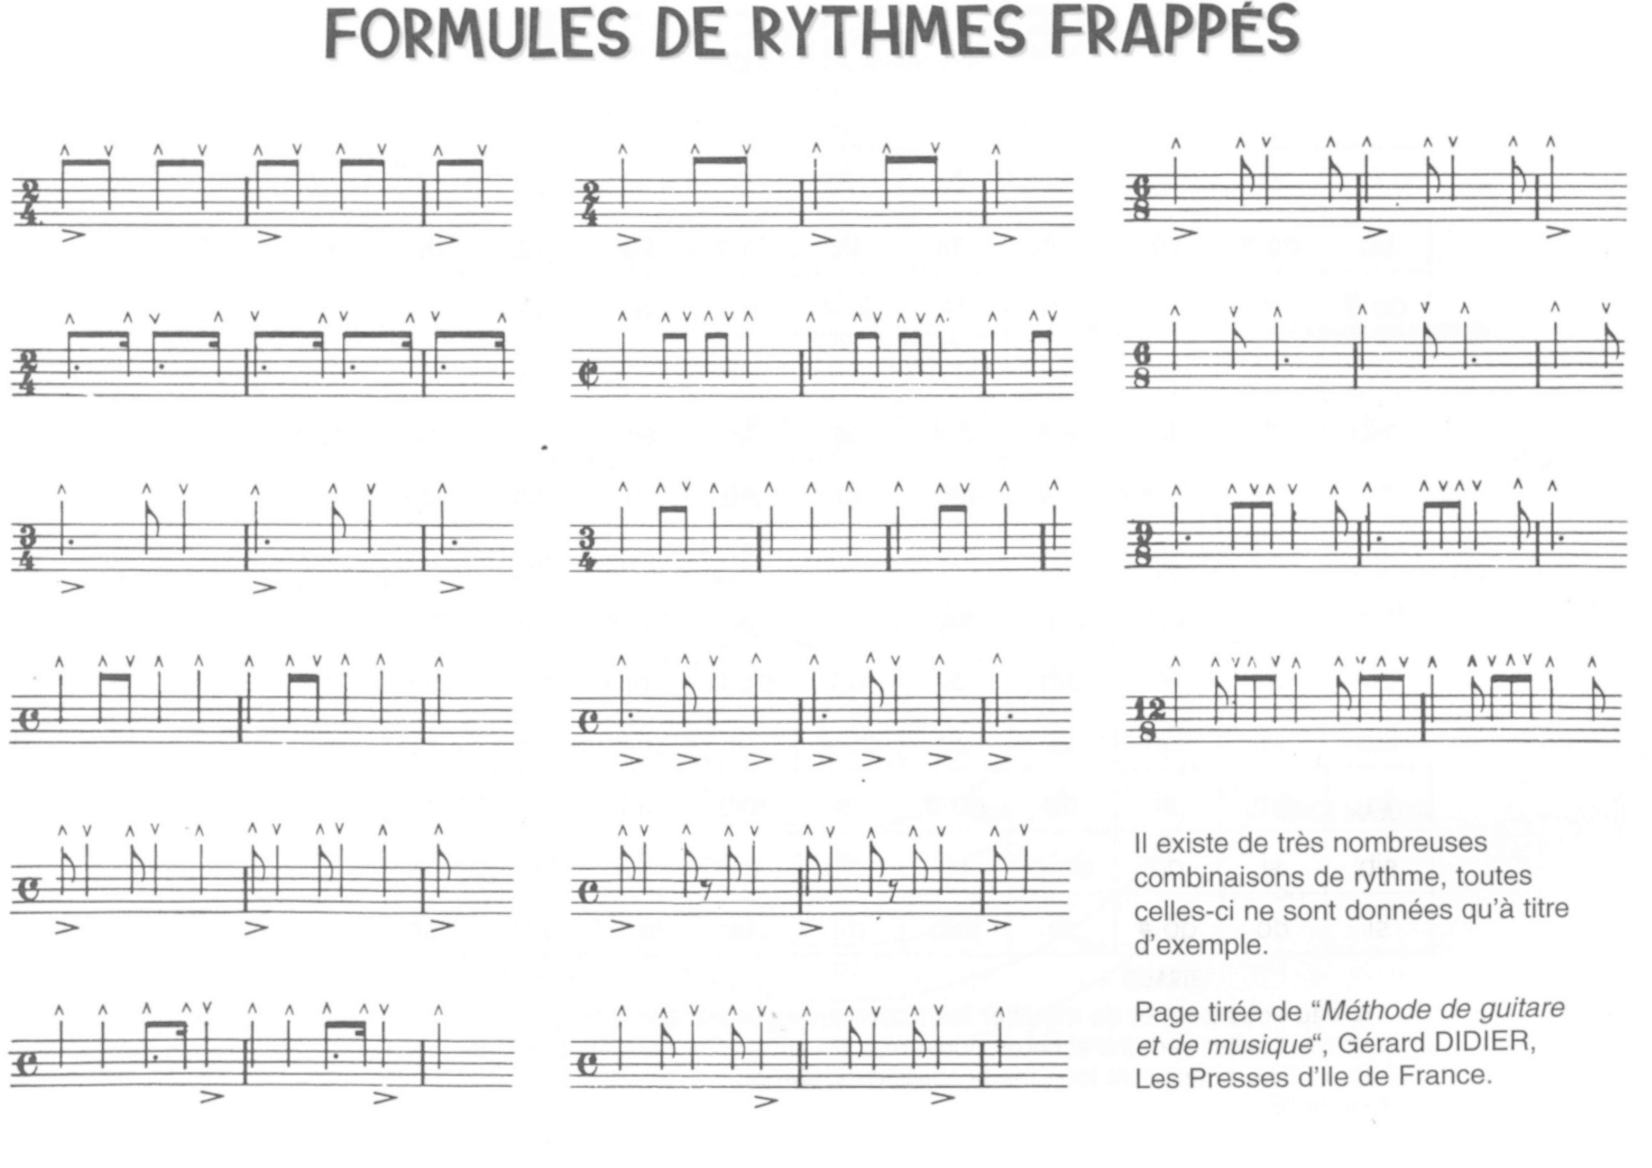
\includegraphics[width=.95\linewidth]{photos_accords/rythmes.png}
\end{figure}

\begin{figure}[ht!]
    \centering
    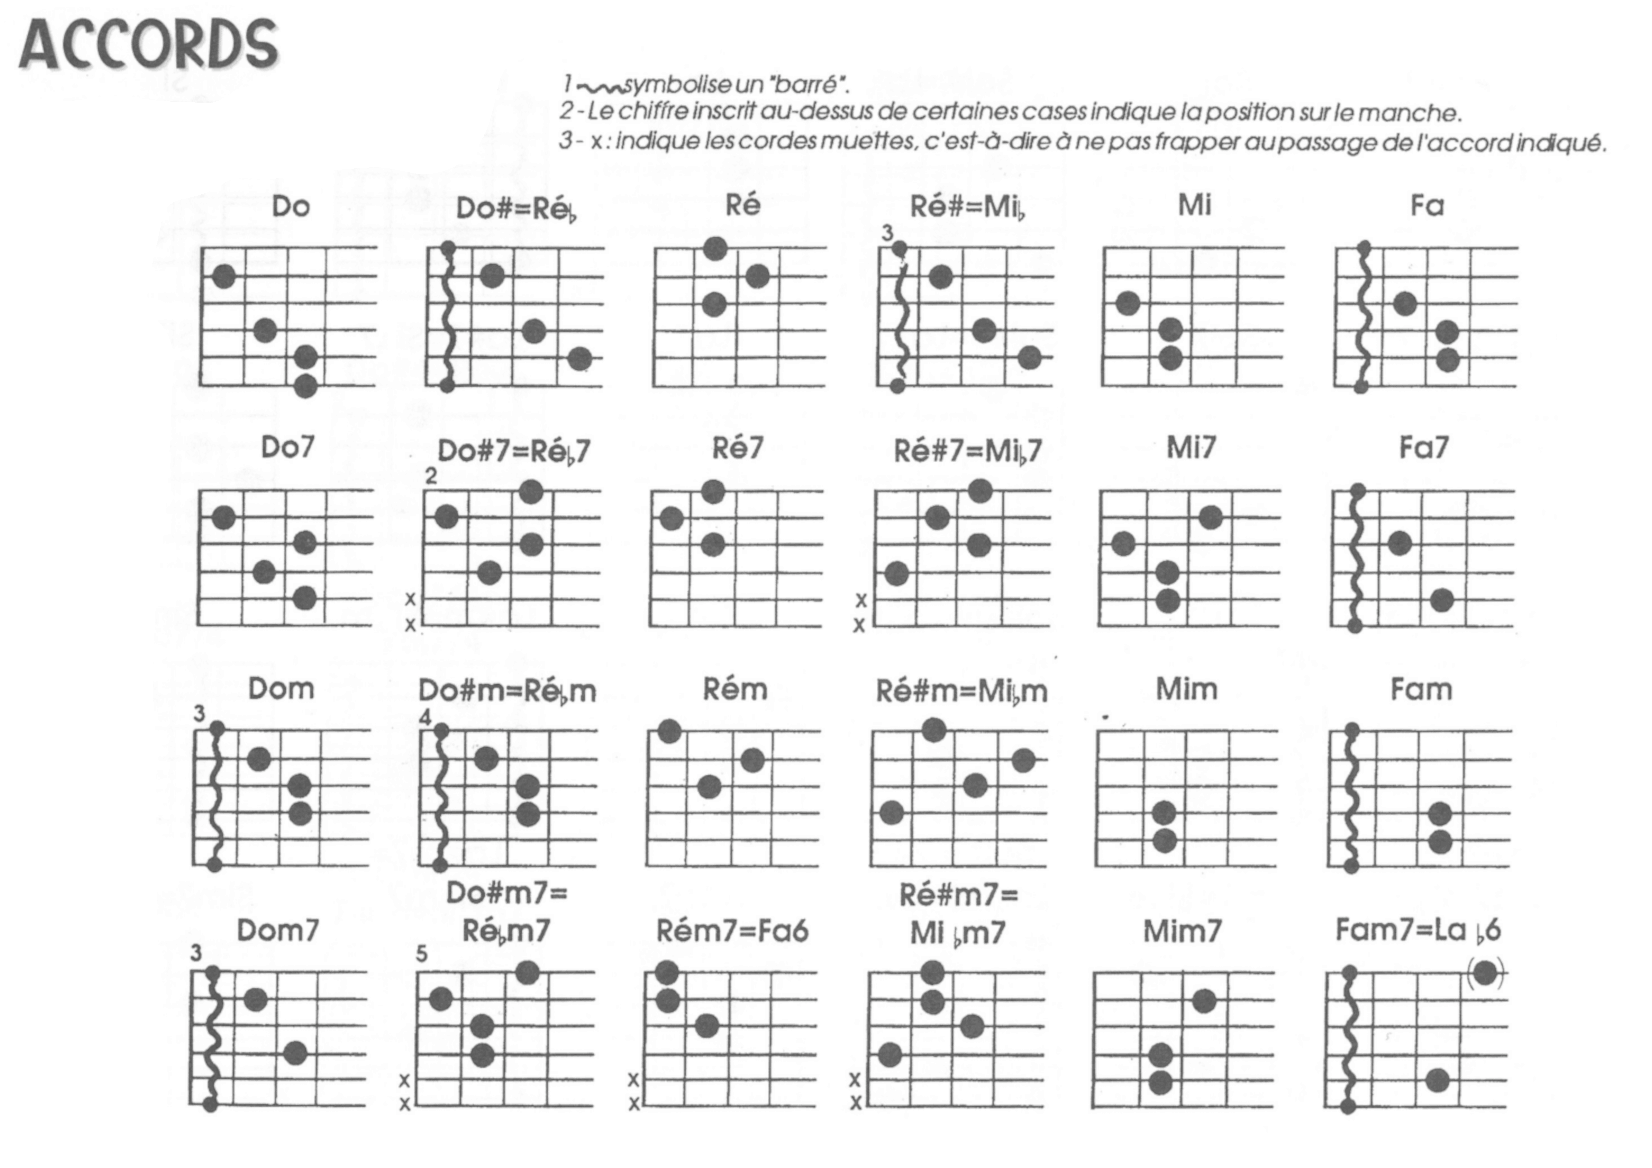
\includegraphics[width=.95\linewidth]{photos_accords/accords_1.png}
\end{figure}
\begin{figure}[ht!]
    \centering
    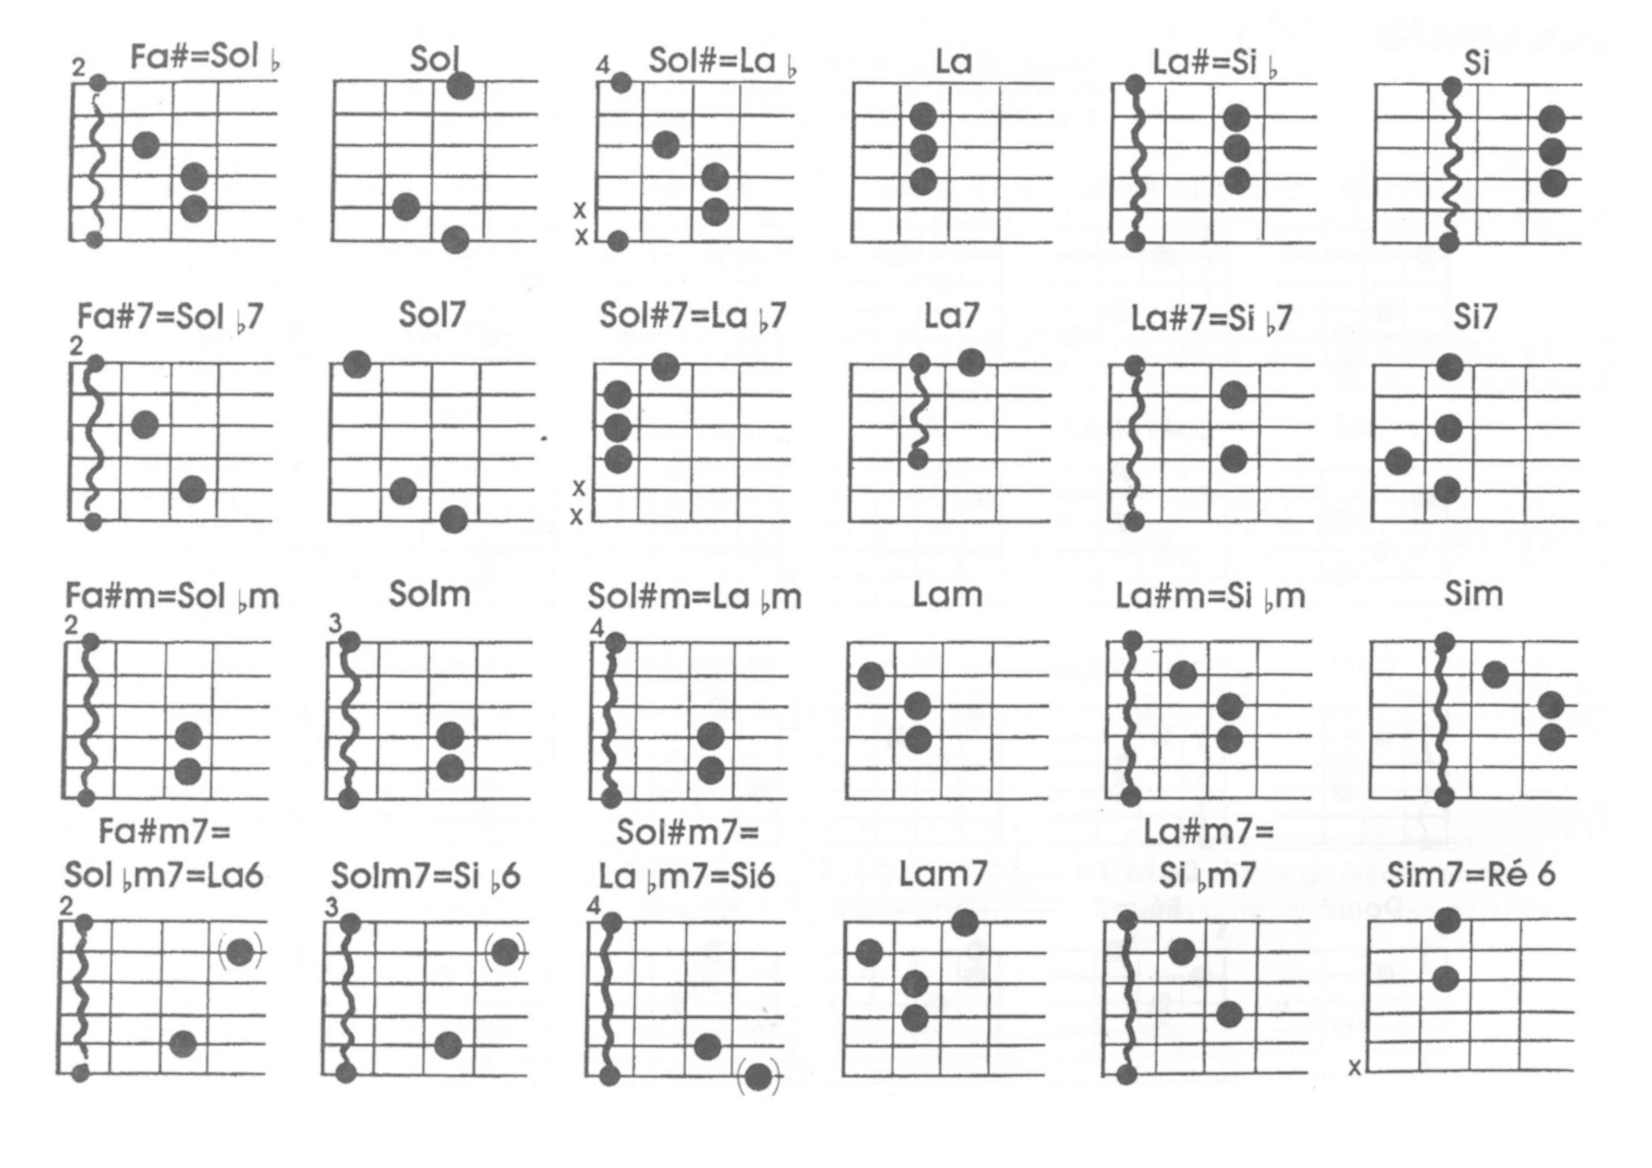
\includegraphics[width=.95\linewidth]{photos_accords/accords_2.png}
\end{figure}
\begin{figure}[ht!]
    \centering
    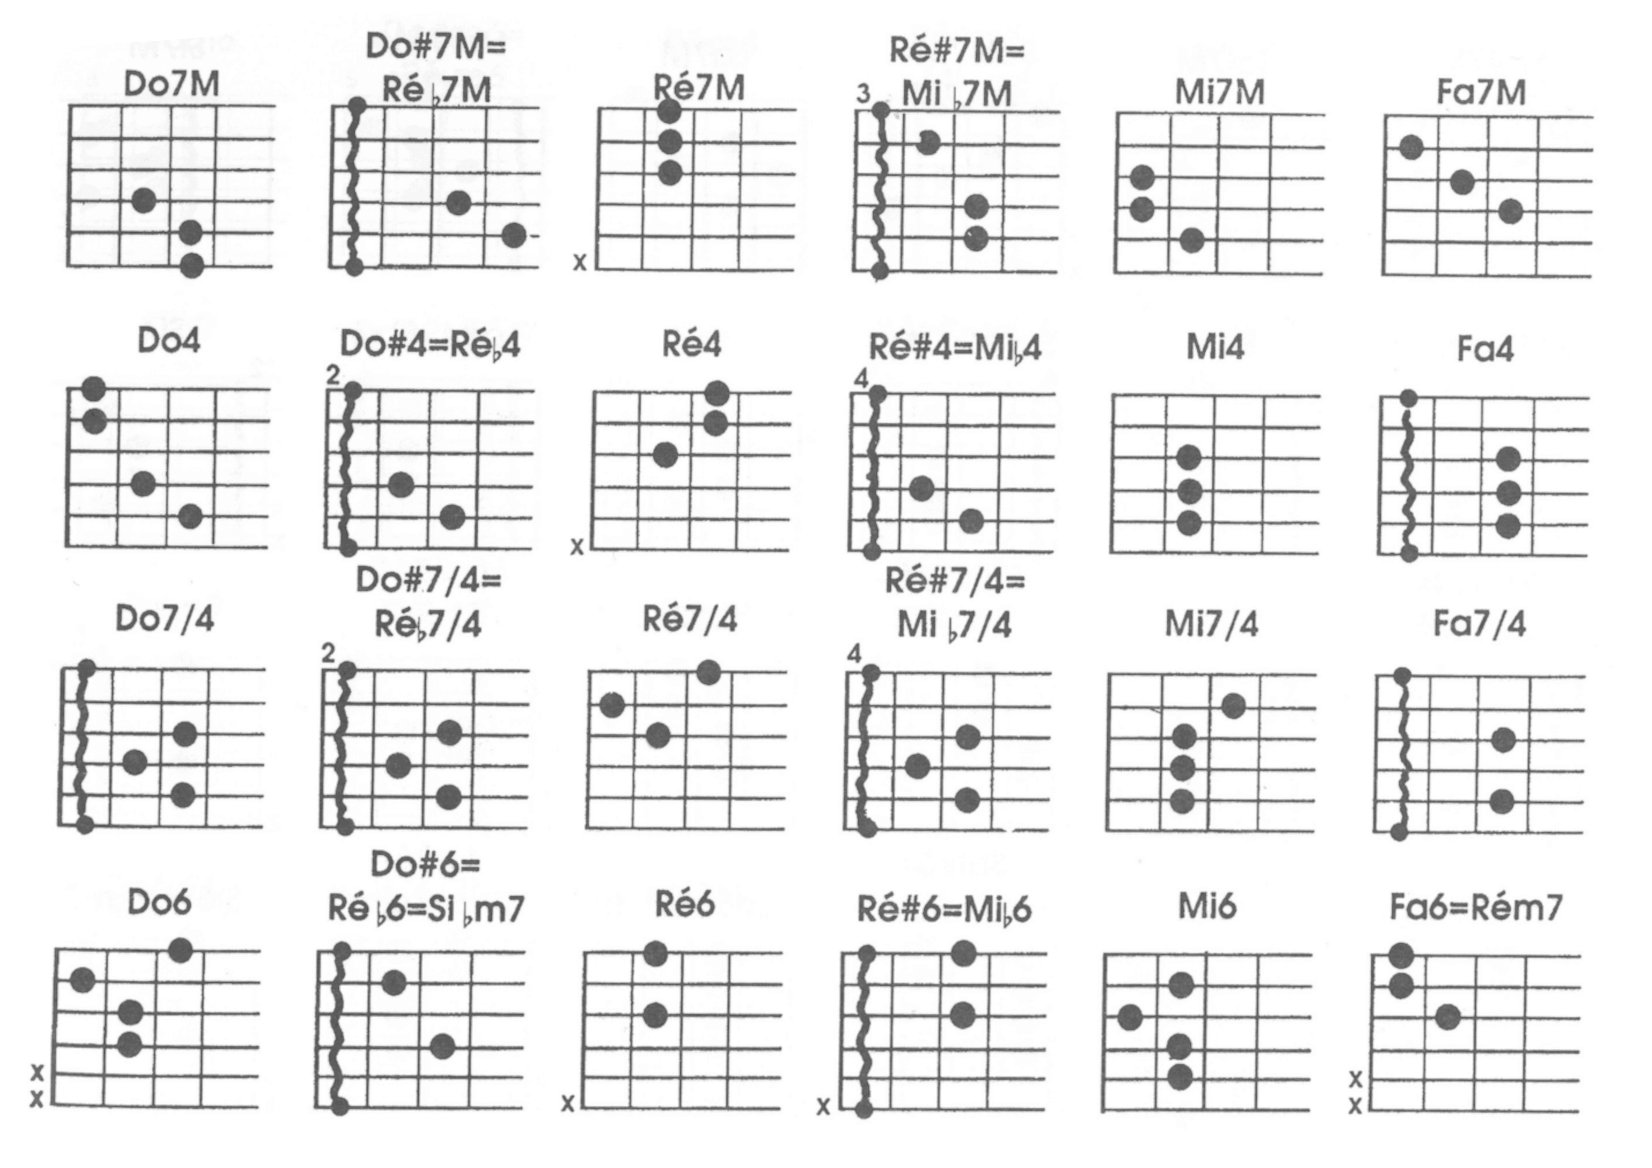
\includegraphics[width=.95\linewidth]{photos_accords/accords_3.png}
\end{figure}
\begin{figure}[ht!]
    \centering
    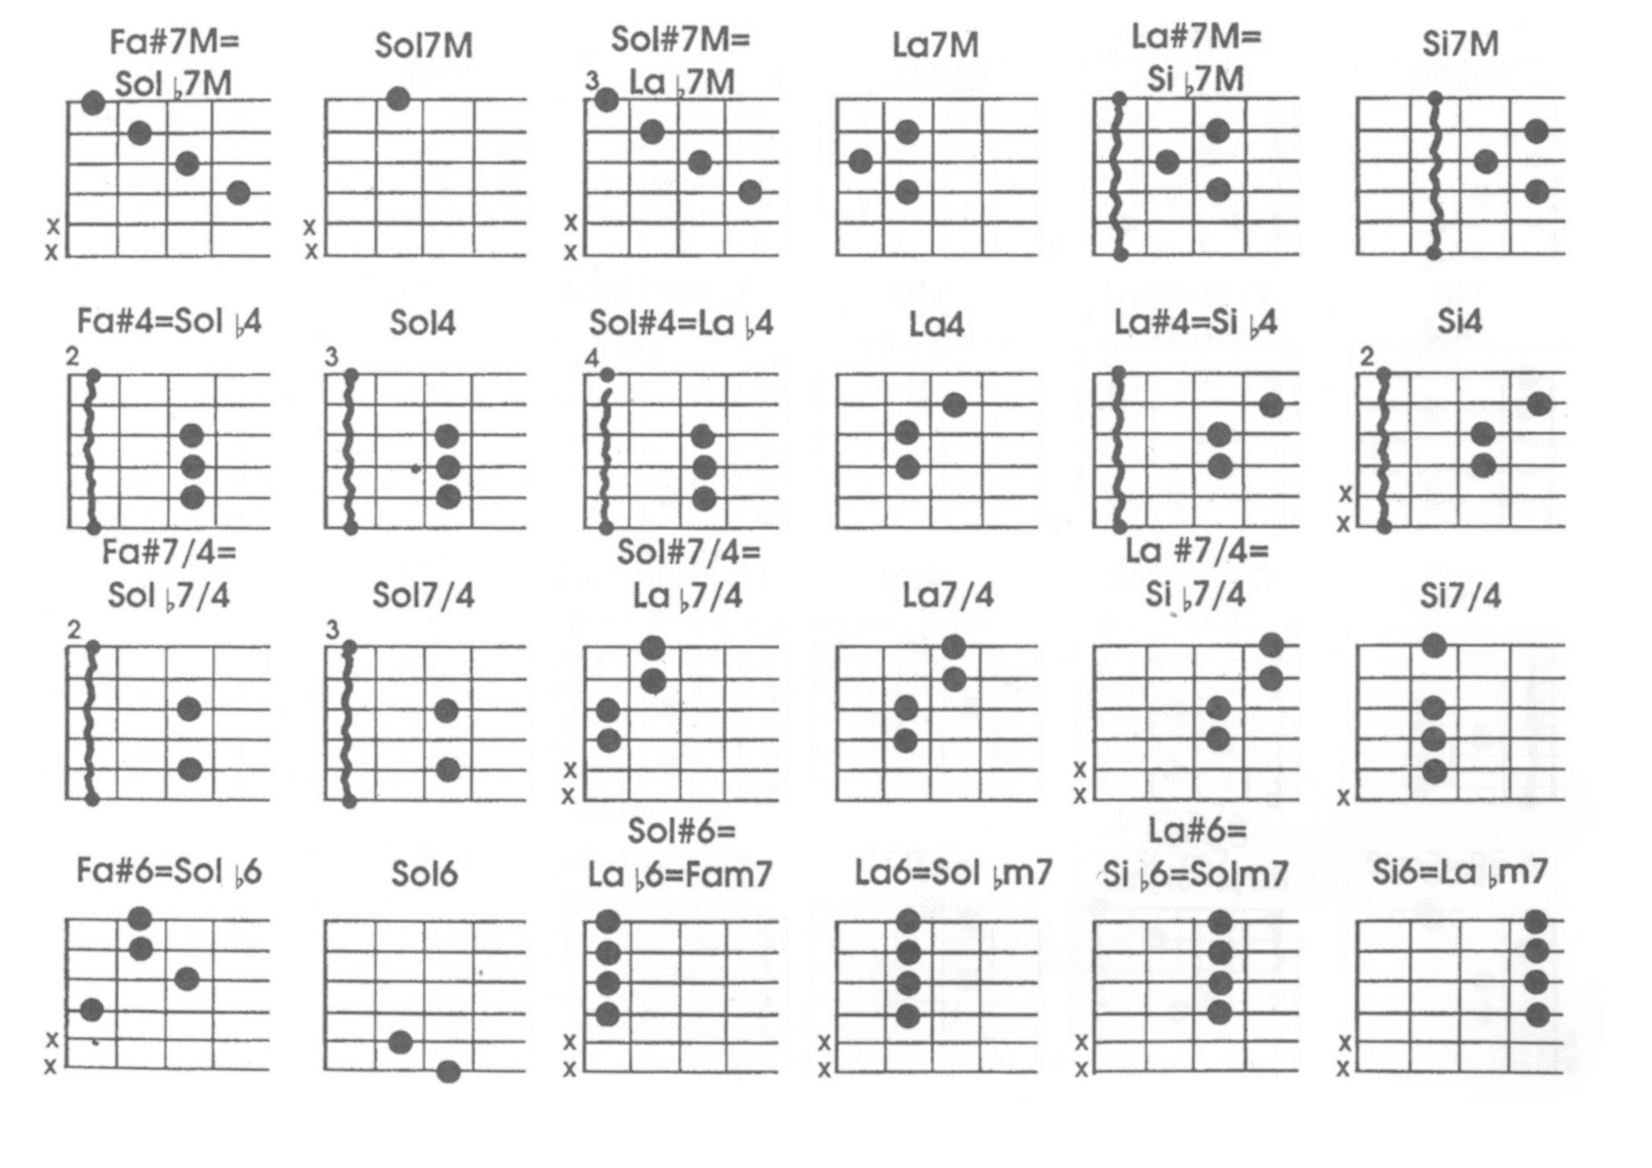
\includegraphics[width=.95\linewidth]{photos_accords/accords_4.png}
\end{figure}
\begin{figure}[ht!]
    \centering
    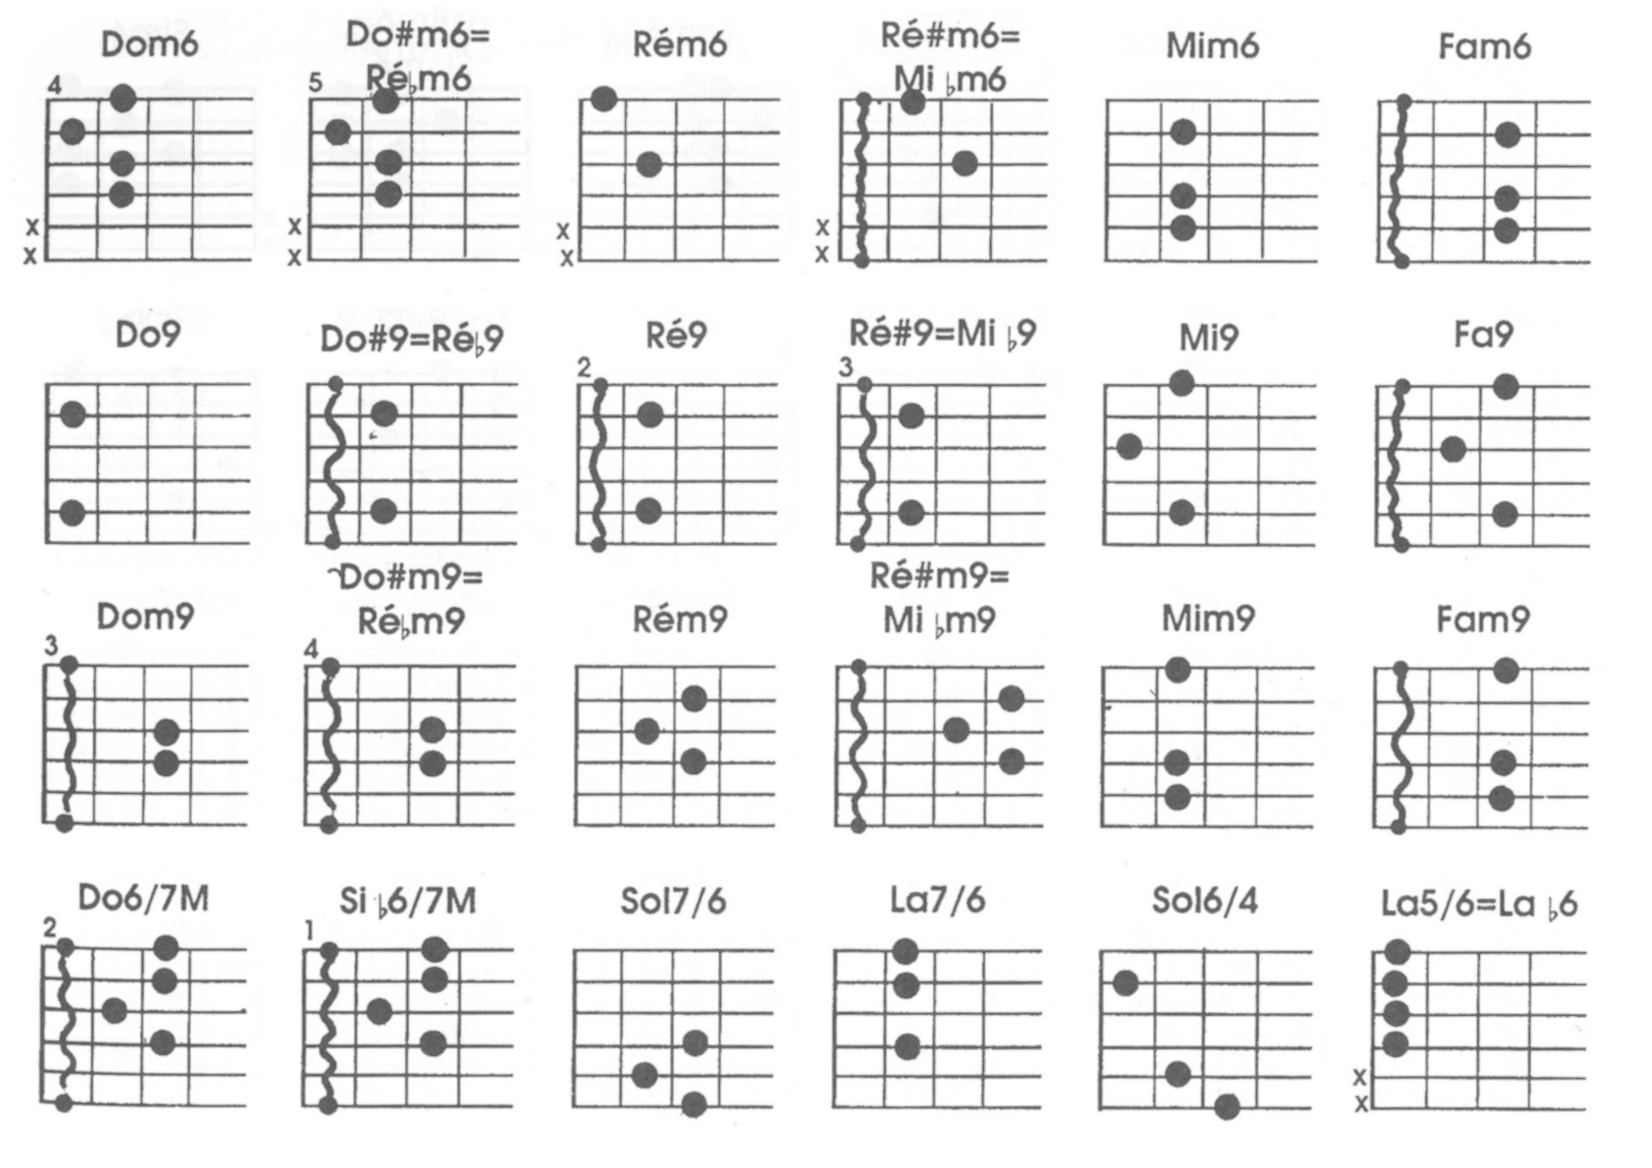
\includegraphics[width=.95\linewidth]{photos_accords/accords_5.png}
\end{figure}
\begin{figure}[ht!]
    \centering
    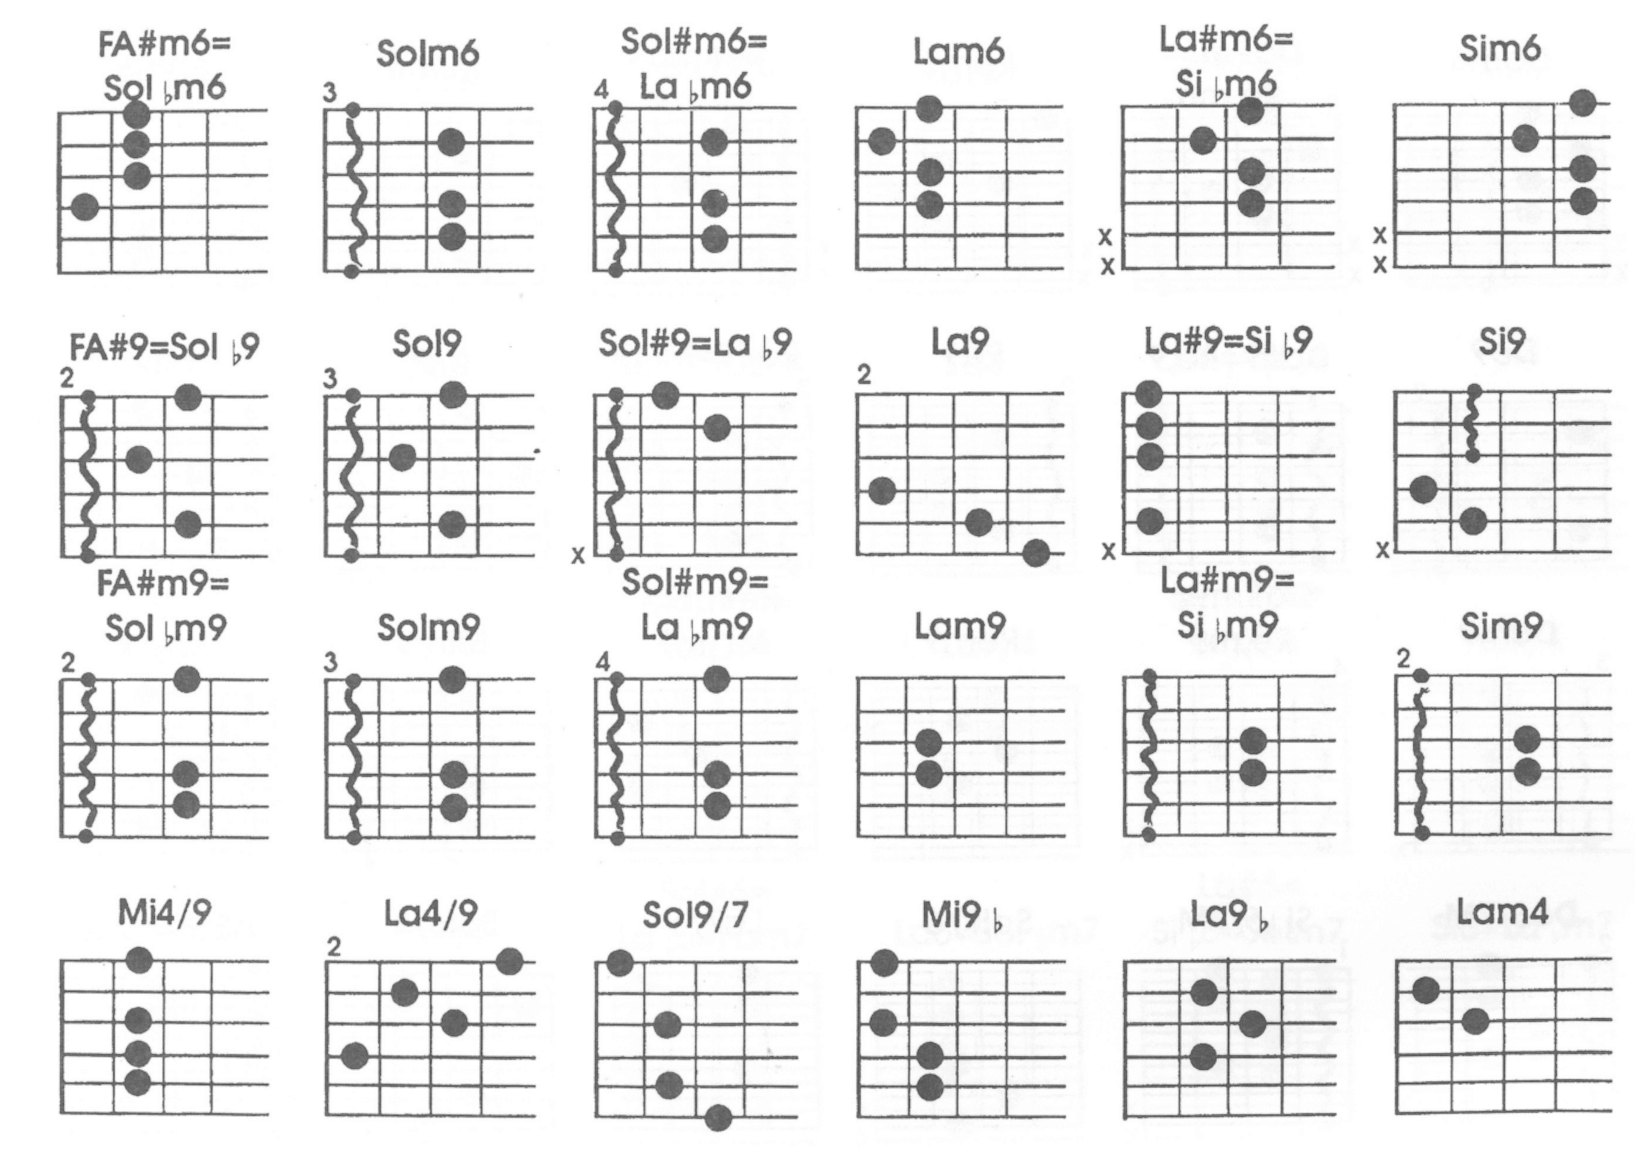
\includegraphics[width=.95\linewidth]{photos_accords/accords_6.png}
\end{figure}
\begin{figure}[ht!]
    \centering
    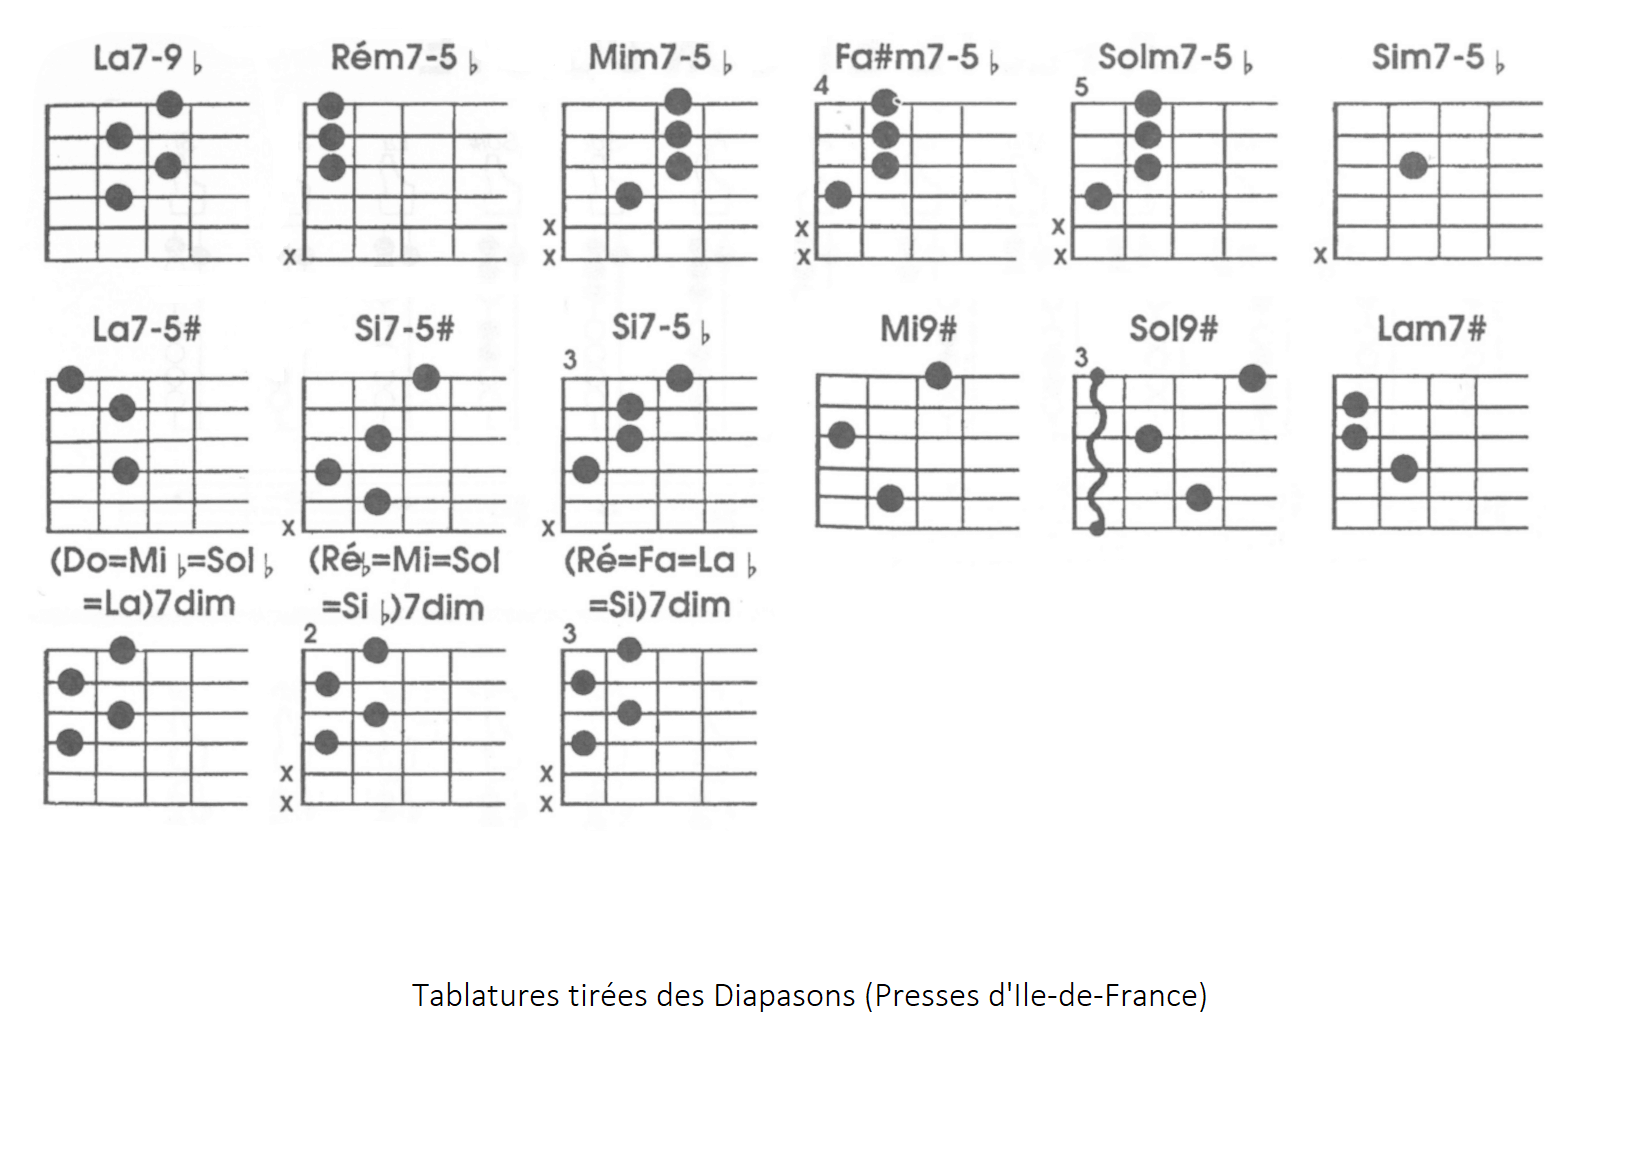
\includegraphics[width=.95\linewidth]{photos_accords/accords_7.png}
\end{figure}

\end{document}


